\documentclass[11pt,oneside]{book}

\usepackage{textcomp}
\usepackage{amsfonts}
\usepackage{amsmath}
\usepackage{amssymb,bm}
\usepackage{gensymb}
\usepackage{graphicx,color}
%\usepackage{subfigure}
\usepackage{subfig}
\usepackage{caption}
\usepackage[spanish]{babel}
\usepackage{float}
\usepackage[left=4cm,right=2.5cm,top=2.5cm,bottom=2.5cm,headheight=35pt]{geometry}
\DeclareGraphicsExtensions{.pdf,.png,.jpg}
\usepackage{url}
\usepackage[title]{appendix}
\usepackage[T1]{fontenc}
\usepackage{xcolor}
\usepackage{longtable}

\setcounter{secnumdepth}{5}
\setcounter{tocdepth}{5}
\usepackage{hyperref}
\hypersetup{
    colorlinks=true,
    linkcolor=black,
    filecolor=black,
    citecolor=black,
    urlcolor=black,
    pdftitle={},
    pdfsubject={},
    pdfauthor={},
    pdfkeywords={}
}

% INICIO***********paquetes de dibujo*******
\usepackage{tikz}
\usepackage{tikz-3dplot}
\usepackage{pst-all}	%call the pstricks package
\usepackage{pst-3dplot}
\usepackage{pst-solides3d}
%\newpsobject{malla}{psgrid}{subgriddiv=1,griddots=10,gridlabels=6pt}
% FIN***********paquetes de dibujo*******

\usetikzlibrary{shapes,snakes}
\usetikzlibrary{arrows,shapes,positioning,shadows,trees}
\usetikzlibrary{trees,positioning,shapes,shadows,arrows}
\usetikzlibrary{calc}

\usepackage[edges]{forest}
\usepackage{svg}

\usepackage{comment}
\usepackage{multirow,array}
\usepackage[singlespacing]{setspace}
\usepackage{fancyhdr}
\usepackage{fancybox}
\usepackage{import}
\usepackage[scale=1.2]{ccicons}
\usepackage{booktabs}
\usepackage{xspace}
\usepackage[utf8]{inputenc}
\usepackage[style=spanish]{csquotes}
\usepackage{subfig}
\usepackage{tabularx}

\usepackage{xcolor}
\usepackage[linesnumbered,ruled,vlined]{algorithm2e}
\usepackage{enumerate}
\usepackage{stackengine}
\usepackage{smartdiagram}  
\usepackage{svg}

\usepackage{caption}
\usepackage{listings}
\usepackage[newfloat]{minted}
\usepackage{caption}
\newenvironment{code}{\captionsetup{type=listing}}{}
\SetupFloatingEnvironment{listing}{name=Source Code}
%\renewcommand\listoflistingscaption{Lista de fragmentos de códigos}
%\renewcommand\listingscaption{Código}

%% minted
\setminted{frame=lines,
                                breaklines=true,
                                breaksymbolleft=,
                                framesep=2mm,
                                baselinestretch=1.2,
                                bgcolor=LightGray,
                                fontsize=\footnotesize,
                                linenos}

%%%   XML %%%   
\usepackage{lmodern}
\usepackage{listings}

\usepackage{color}
\definecolor{gray}{rgb}{0.4,0.4,0.4}
\definecolor{darkblue}{rgb}{0.0,0.0,0.6}
\definecolor{cyan}{rgb}{0.0,0.6,0.6}

\lstset{
basicstyle=\ttfamily,
columns=fullflexible,
showstringspaces=false,
commentstyle=\color{gray}\upshape,
escapechar=* % <=  to escape to LaTeX
}
\lstdefinelanguage{XML}
{
backgroundcolor = \color{orange!5},
breaklines=true,
  morestring=[b]",
  morestring=[s]{>}{<},
  morecomment=[s]{<?}{?>},
  stringstyle=\color{black},
 identifierstyle=\color{darkblue},
 keywordstyle=\color{cyan},
 morekeywords={xmlns,version,type}% list your attributes here
 }
 
 
 \lstdefinelanguage{msg}
{
backgroundcolor = \color{lightblack},
breaklines=true,
  stringstyle=\color{white},
 identifierstyle=\color{white},
 keywordstyle=\color{white},
  xleftmargin=.2\textwidth, xrightmargin=.3\textwidth,
 }

\definecolor{LightGray}{gray}{0.9}
\definecolor{DarkGray}{gray}{0.1}

\usemintedstyle{borland}
%%%% Bibliografia Referencias %%%   
%\usepackage[backend=biber]{biblatex}
%\addbibresource{Back/References.bib}
%\usepackage{mathtools}
%\parskip=2pt

\usepackage[spanish]{babel} 
\usepackage[backend=biber, style=iso-numeric]{biblatex}
\addbibresource{Back/References.bib}
\usepackage{mathtools}
\parskip=2pt

\usepackage{url}

\usepackage{empheq}

%%% PYHTON
\usepackage[T1]{fontenc}
\usepackage[utf8]{inputenc}
\usepackage{minted}
\usepackage{listings}

\renewcommand{\rmdefault}{phv}
\renewcommand{\sfdefault}{phv}
\sffamily


\pagestyle{fancy}
\lhead{}
\chead{}
\rhead{}
\renewcommand{\headrulewidth}{0.pt}
\cfoot{}
\rfoot{\thepage}
\renewcommand{\footrulewidth}{0.pt}

\makeatletter

% \let\plainappendixpage\appendixpagename
% \makeatletter
% \renewcommand{\appendixpage}{
%   \begingroup
%   \let\ps@plain\ps@empty
%   \plainappendixpage
%   \endgroup}
% \makeatother

\graphicspath{
{Main/Chapter1/Images1/}
{Main/Chapter2/Images2/}
{Main/Chapter3/Images3/}
{Main/Chapter4/Images4/}
{Main/Chapter5/Images5/}
{Main/Chapter6/Images6/}
{Main/Chapter7/Images7/}
{Main/Chapter8/Images8/}
{Front/Images}
{Back/Images}
}

\definecolor{ruddybrown}{rgb}{0.73, 0.4, 0.16}
\definecolor{russet}{rgb}{0.5, 0.27, 0.11}

\begin{document}
	
\singlespacing
\renewcommand{\contentsname}{Tabla de Contenido}
%\hypersetup{    
%    colorlinks=true,        
%    linkcolor=blue,         
%    filecolor=magenta,       
%    urlcolor=russet,           
%    citecolor=blue
%}                           

\renewcommand{\listtablename}{Índice de Tablas}
\renewcommand{\listfigurename}{Índice de Figuras}
\renewcommand{\bibname}{Bibliografía}
\renewcommand{\tablename}{\small\bf Tabla}
\renewcommand{\figurename}{\small\bf Figura}
\newcommand{\paginiciales}[1]{\begin{center}\begin{huge}\textbf{#1}\end{huge}\end{center}}
\renewcommand{\appendixname}{Apéndice}
\renewcommand{\appendixtocname}{APÉNDICE}
\renewcommand{\appendixpagename}{APÉNDICE}
\newcommand\tr{\rule{0pt}{4.5ex}}
\newcommand\br{\rule[-3ex]{0pt}{3ex}}

{
\newgeometry{top=40mm}

\fontfamily{phv}\selectfont

\thispagestyle{empty}

\begin{tabular}{p{12.1cm}p{3cm}}
\begin{center}
\onehalfspacing{
\vspace{-1cm}
\LARGE{\textbf{UNIVERSIDAD DE SANTIAGO DE CHILE}}\\
\Large{\textbf{FACULTAD DE INGENIERÍA\\ Departamento de Ingeniería Mecánica}}
}
\end{center}
&
\vspace{-1.5cm} \hspace{-1cm}

\includegraphics[scale=1]{Front/Images/usach-color.pdf}
\end{tabular}


\begin{center}
\vspace{9\baselineskip}


\onehalfspacing{\large{\textbf{VALIDACIÓN DE MODELACIÓN CINEMÁTICA Y DINÁMICA DE UN ROBOT DELTA 3 GDL A TRAVEZ DE ROS Y ADAMS   }}}

\vspace{3\baselineskip}

\small {\textbf{Iván Alejandro Fernández Gracia \\ Rodrigo Eduardo Soto Castro}}
\end{center}

\vspace{4\baselineskip}

\begin{flushright}
\begin{minipage}{7cm}
\small{Profesor guía: \\ Michael Gabriel Miranda Sandoval}
\end{minipage}
\end{flushright}

\vspace{0.5\baselineskip}

\begin{flushright}
\begin{minipage}{7cm}
\small{Trabajo de Titulación presentado en conformidad a los requisitos para obtener el Título de Ingeniero Civil en Mecánica.}
\end{minipage}
\end{flushright}

\vspace{3\baselineskip}

\begin{center}
\begin{minipage}[c]{15cm}
\centering
\small{Santiago $-$ Chile \\ 2020}
\end{minipage}
\end{center}

\restoregeometry
}

{
\thispagestyle{empty}
\vspace*{18.5cm}

\begin{flushleft}
\textbf{\copyright} \hspace{0.08cm} \textbf{Iván Alejandro Fernández Gracia, 2020}\\
\textbf{\copyright} \hspace{0.08cm} \textbf{Rodrigo Eduardo Soto Castro, 2020}
\end{flushleft}
\vspace{0.5cm}


}



\frontmatter 
\pagenumbering{roman}


\phantomsection  
\thispagestyle{fancy}
\paginiciales{RESUMEN}
\addcontentsline{toc}{chapter}{RESUMEN}
\vspace{5mm}
En el presente trabajo se realiza un análisis numérico del comportamiento dinámico de partículas esféricas rígidas pertenecientes a un nanofluido, siendo agua el fluido base, en régimen laminar y térmicamente desarrollado en microcanales de sección rectangular. Producto de los campos de velocidades, presiones y temperaturas impuestos, las nanopartículas hacen contacto entre ellas y con las paredes.

El presente trabajo es un estudio de los algoritmos de generaci´on y planificaci´on de  trayectorias  para  robots  m´oviles  de  configuraci´on  diferencial  y  su  comparaci´on bajo ´ındices de desempen˜o.

Para  este  trabajo  de  t´ıtulo,  se  aborda  la  configuraci´on  cinem´atica  de  los  robot m´oviles,  controladores  para  el  movimiento  del  robot,  algoritmos  de  planificaci´on  y generaci´on de trayectorias DFS, Hill Climbing y A*, y la complejidad de estos.

Se comparan los algoritmos mediante simulaciones en MatLab y Simulink, pro- gramando una interfaz gr´afica de usuario (GUI) y comparando la distancia, tiempo y velocidad con que los algoritmos obtienen una trayectoria sobre un terreno con obst´aculos.

A partir de los resultados, se concluye que el algoritmo A* es o´ptimo con respecto a la trayectoria generada, el algoritmo DFS obtiene las trayectorias en menor tiempo y el algoritmo Hill Climbing genera trayectorias de menor distancia que DFS y en menor tiempo que A*.

Presentación v
PRESENTACIÓN
El presente trabajo se centra en el estudio de los componentes léxico y
morfosintáctico del lenguaje en pacientes afásicos bilingües del castellano y del
catalán. En este sentido, es relevante destacar dos cuestiones. Por un lado, la
importancia de la investigación relacionada con dichos componentes en el estudio
del procesamiento del lenguaje en pacientes agramáticos. A lo largo de la
literatura se puede encontrar una gran variedad de trabajos que han aportado
información acerca de las alteraciones que presentan los pacientes afásicos
agramáticos en lenguas como el inglés o el italiano. Sin embargo, los déficits que
muestran los pacientes agramáticos en lenguas como el castellano o el catalán han
estado mucho menos estudiados. Por ello, el presente trabajo pretende contribuir
en el conocimiento de cuáles son las dificultades que presentan estos pacientes
agramáticos y si éstas se pueden considerar similares a las presentadas por
pacientes de otras lenguas.
Por otro lado, el interés por el estudio del fenómeno del bilingüismo. No
existen muchos trabajos que relacionen y comparen de una manera detallada y
precisa las alteraciones de los afásicos agramáticos en castellano y en catalán. Por
ejemplo, uno de los objetivos específicos de este trabajo ha sido comprobar si los
pacientes que aquí se han estudiado presentaban patrones de recuperación
similares en castellano y en catalán, por tratarse de lenguas con una estructura
similar. O si, por el contrario, las formas de recuperación presentadas por los
pacientes en ambas lenguas difieren de una forma clara. Ambas cuestiones serán
examinadas tanto en el ámbito de la producción como en el de la comprensión,
aunque haciendo mayor énfasis en el primero.
Para llevar a cabo este estudio, adoptaremos el enfoque de la
Neuropsicología cognitiva, utilizando la metodología de estudio de casos, con la
finalidad principal de estudiar los distintos tipos de alteraciones que presentan los
pacientes. Asimismo, con esta metodología se pretende encontrar disociaciones
(simples o dobles) que contribuyan a estructurar un modelo de procesamiento del
lenguaje en personas sin daño cerebral.
Con el fin de conseguir este objetivo, el presente trabajo se ha estructurado
en seis capítulos además de los apéndices y la bibliografía.
vi Estudio del componente léxico y morfosintáctico en pacientes afásicos bilingües
En el capítulo I, se presenta, a modo de introducción general, un breve
recorrido histórico sobre el tema de la afasia. Dicho recorrido tiene como punto de
inicio los primeros documentos médicos escritos encontrados en los que se
recogían manifestaciones clínicas lingüísticas, pasando por los inicios de la
Neuropsicología Clásica y el localizacionismo con autores destacados como Paul
Broca y Karl Wercnicke; y hasta llegar al desarrollo de la Neuropsicología
Cognitiva en nuestros días.
El capítulo II se compone de tres apartados principales. En el primero, se
aborda el tema del agramatismo desde el enfoque de la Neuropsicología
Cognitiva, presentando una revisión de los trabajos que han investigado acerca de
la sintomatología de los pacientes agramáticos tanto en el ámbito de la producción
como en el de la comprensión. Asimismo, se hace mención de la polémica que
existe actualmente en relación al concepto de agramatismo debido a la
variabilidad de síntomas que presentan los pacientes agramáticos. En el segundo
apartado, debido a que nuestros pacientes presentaron anomia como síntoma en
mayor o menor grado, se incluye una revisión de algunos de los trabajos que han
estudiado la sintomatología de los pacientes anómicos. Y, en tercer y último lugar,
se presenta un apartado dedicado a los modelos teóricos de procesamiento del
lenguaje propuestos por diferentes autores y bajo los cuales se ha pretendido dar
una explicación a la sintomatología afásica.
En el capítulo III se especifica la relación existente entre afasia y
bilingüismo a partir de trabajos de autores como Fabbro o Paradis que han
estudiado a pacientes afásicos bilingües (o multilingües) de distintos dialectos del
italiano o incluso del francés y del inglés. Además, se abordan cuestiones como
por ejemplo los patrones de recuperación de los pacientes o la representación
cerebral de las distintas lenguas.
En el capítulo IV se presentarán los aspectos relacionados con los
objetivos del presente trabajo, así como la metodología empleada. Dentro de la
metodología, se especifican los pacientes estudiados y las tareas que han sido
diseñadas para su administración. Se incluye también el tipo de análisis que
hemos elaborado para clasificar los errores de nuestros pacientes en las diversas
tareas. Si bien hubo un grupo determinado de tareas que se administraron a todos
los pacientes de forma general, otras tareas no pudieron pasarse a todos los
Presentación vii
pacientes debido a las dificultades que tuvimos para acceder a algunos de ellos, ya
fuera por recaídas de la enfermedad como por la negación del paciente a seguir
colaborando.
El capítulo V corresponde a los resultados obtenidos en el análisis de las
tareas realizadas por los pacientes que han participado en el presente trabajo.
Puesto que tres de los cinco pacientes que formaron parte de la muestra eran
bilingües, la descripción de los resultados de estos pacientes se realizó en dos
bloques. En un primer bloque se describen los resultados obtenidos a partir de la
administración de las tareas en la primera lengua del paciente (que en todos los
casos coincidió ser el catalán), y en un segundo bloque se presentan los resultados
obtenidos a partir del análisis de las tareas en la segunda lengua de los pacientes
(castellano). En la exposición de cada paciente se ha incluido una breve
presentación de la historia médica y social, los resultados obtenidos en una
primera evaluación clínica del lenguaje y, finalmente el análisis de las pruebas
experimentales. Si bien en este trabajo se ha prestado una atención especial al
análisis cualitativo de los datos por tratarse de una metodología de estudio de caso
único, también se han realizado análisis cuantitativos. Asimismo, en este capítulo
se incluye la discusión de los resultados obtenidos para cada paciente en base a
los modelos teóricos anteriormente mencionados.
En el capítulo VI y último, se presentan las principales conclusiones
generales que se han obtenido a partir de la realización de este trabajo.
\vfill
\noindent\textbf{Palabras clave:} Robot Delta, Robot Operating System, ROS, ADAMS, Robot Paralelo, Cinematica, Dinamica, Jacobiano, Rviz, Espacio de Trabajo, Robótica.

\phantomsection 
\thispagestyle{fancy}
\paginiciales{ABSTRACT}
\addcontentsline{toc}{chapter}{ABSTRACT}
\vspace{5mm}
Forma objetiva, breve y específica del contenido del trabajo realizado. Su extensión no debe superar las 300 palabras. 
En el caso de las tesis de magister debe incluir un Abstract en hoja aparte.
Palabras claves: incluir 3 o 4 palabras o frases que indiquen el contenido temático de la investigación.

\vfill
\noindent\textbf{Keywords: Delta Robot, Robot Operating System, ROS, ADAMS, Parallel Robot, Kinematics, Dynamics, Jacobian, Rviz, Workspace.} 
\phantomsection  
\thispagestyle{fancy}
\paginiciales{DEDICATORIA}
\addcontentsline{toc}{chapter}{DEDICATORIA}

\vspace{5cm}

\begin{flushright}
{
{\sc  A mis padres Marcelo y Marcela}\\
{\sc  A mi hermana María}\\
{\sc  A mis abuelos Luis y Adela}\\
{\sc  A mis familiares}\\
{\sc  A mis grandes amigos}\\
}
\end{flushright}
\begin{flushright}
{
{\sc \textbf{Atentamente, Iván Alejandro Fernández Gracia}} \\
}
\end{flushright}

\begin{flushright}
{
{\sc  A mis padres }\\
{\sc  A mi hermana }\\
{\sc  A mis abuelos}\\
{\sc  A mis }\\
{\sc  A mis }\\
}
\end{flushright}
\begin{flushright}
{
{\sc \textbf{Atentamente, Rodrigo Eduardo Soto Castro}} \\
}
\end{flushright}







\vfill
\begin{centering}
{{\textit{Zeroth Law:} ``{\it A robot may not harm humanity, or, by inaction, allow humanity to come to harm.}''}\\
{\sc Isaac Asimov (1920 - 1992)}\\}
\end{centering}




\phantomsection  
\thispagestyle{fancy}
\paginiciales{Agradecimientos}
\addcontentsline{toc}{chapter}{Agradecimientos}

\vspace{5mm}

Este trabajo de título realizado en la Universidad de Santiago de Chile es un esfuerzo en el cual, directa o indirectamente, participaron varias personas. Es por eso que dedico unas palabras a todas estas personas que me acompañaron en este largo camino.

En primer lugar agradecer a los profesores Michael Miranda, Héctor Muñoz y Ricardo Manríquez, quienes me motivaron a introducirme en el área de la robótica.  

Agradecer  al profesor Francisco Sepúlveda Palma, quien fue uno de los primeros académicos que confió en mi como alumno y persona. Me ofreció realizar mi primera ayudantía importante en mi carrera.

A mis amigos de universidad, Raul, Alejandro, Cristian, Claudio y  Elias por las risas y alegrías que vivimos en los pasillos de la universidad.

Un especial agradecimiento a Pedro Godoy, mi profesor del colegio Ingles Saint Jonh de Rancagua, quien fue el principal responsable de mi formación matemática y me salvo de ser una persona rebelde.

A mis amigos y amigas, Juan Andres, Jose Miguel, Nicolás, Lucas, Pablo, Sebastian, Chung Chii, Javier, Nataly, Camila Alejandra y Maria Fernanda por distraerme de mis estudios para disfrutar de la vida y por estar junto a mi en los momentos que mas necesitaba apoyo.     

A mi hermana Maria, por soportar mi desorden en el departamento donde vivíamos. 

A mis padres Marcelo y Marcela, por alimentarme, preocuparse por mi educación y darme amor incondicional.


\begin{flushright}
{
{\sc \textbf{\textit{Atentamente, Iván Alejandro Fernández Gracia}}} \\
}
\end{flushright}



%\begin{flushright}
%{
%{\sc \textbf{\textit{Atentamente, Rodrigo Eduardo Soto Castro}}} \\
%}
%\end{flushright}

%-------------{List Caps}----------------------------
\addtocontents{toc}{\protect\thispagestyle{fancy}} 
{\hypersetup{colorlinks=black,        
    linkcolor=black}
\tableofcontents
}
\addcontentsline{toc}{chapter}{Tabla de Contenido}%\newpage
\newpage
%------------------{List Tables}----------------------
\addtocontents{lot}{\protect\thispagestyle{fancy}} 
%\listoftables
{
\let\oldnumberline\numberline
\renewcommand{\numberline}{Tabla~\oldnumberline}
\listoftables
}
\addcontentsline{toc}{chapter}{Índice de Tablas}%\newpage
\newpage
%-------------{List of Figure}----------------------------
\addtocontents{lof}{\protect\thispagestyle{fancy}} 
{
\let\oldnumberline\numberline
\renewcommand{\numberline}{\figurename~\oldnumberline}
\listoffigures
}
\addcontentsline{toc}{chapter}{Índice de Figuras}%\newpage

\onehalfspacing
\mainmatter 
\newpage
%-------------{List of Algorithms}----------------------------
%\addtocontents{lof}{\protect\thispagestyle{fancy}} 
%\addcontentsline{toc}{chapter}{Índice de Algoritmos}
%\listofalgorithms
%\newpage

%---------------{Incluir Capitulos}-------------------------
{\hypersetup{colorlinks=true,        
    linkcolor=blue,         
    filecolor=magenta,       
    urlcolor=russet,           
    citecolor=blue}
%\chapter{Introducción}\label{CAP1}

\section{Motivación}

Desde el año 2010 las ventas de robots industriales se han acelerado considerablemente en nuestro país debido a la tendencia continua hacia la automatización y las sucesivas mejoras técnicas en este tipo de sistemas. El estudio de la IDC Worldwide Semiannual Robotics Spending Guide \eqref{} indica que el mercado de la robótica en Latinoamérica presenta un crecimiento en 2019 del 73\% en robots industriales, del 27\% en robots de servicios y de un 0,09\% en robots de consumo. Los robots para producción de alimentos ganan terreno debido a la alta demanda de mano de obra para el trabajo dentro de esta actividad. Sin embargo, este nuevo interés por parte de la industria no se refleja en los estudios y objetivos de las formaciones académicas en las universidades, demostrando nuevamente una de las principales debilidades de nuestro país, la desconexión entre la industria y la academia. Esta desconexión se hace más latente aún con miras a nuestro departamento de mecánica en la USACH, una búsqueda sencilla de la palabra clave “robot” en los repositorios digitales de nuestra universidad, no arroja más de una treintena de resultados posibles, la mayoría de ellos ligados a otros departamentos de la universidad, principalmente eléctrica.

A pesar de esto y con la formación de ingenieros a nuestras espaldas, entendemos que una idea o solución a una problemática, es necesaria adaptarla a la realidad del entorno, en nuestro caso una robótica adaptada a las necesidades y capacidades del país. Es por esto que se elige entre las múltiples ramas de la robótica, los robots de tipo industrial adoptando la definición de la ISO como “Manipulador multifuncional reprogramable con varios grados de libertad, capaz de manipular materias, piezas, herramientas o dispositivos especiales según trayectorias variables programadas para realizar tareas diversas.” Nos enfocaremos en un robot manipulador de tipo delta, con la esperanza de que en un futuro próximo pueda implementarse y ser de ayuda en la industria agropecuaria de nuestro país, específicamente en sus procesos de packing y pick and place.

La intención de esta tesis es revertir este escenario en nuestro departamento, y renovar las iniciativas en el ámbito de la robótica en nuestros compañeros presentando una guía completa, de todos los ámbitos necesarios para comenzar a desarrollar un proyecto de robot delta, mostrando y resolviendo las problemáticas asociadas a la cinemática y dinámica del robot, la matemática implícita en estas soluciones y el código mediante el cual se llegó a dichas soluciones. Además, se realizarán simulaciones que comprueben los resultados teóricos. Todo esto bajo un ambiente de software libre y presentando muchos ramales para posibles proyectos en el área.

\section{Hipótesis de estudio}
Es posible realizar el modelamiento de la cinemática y dinámica de un robot delta a través de softwares libres y validarlo por medio de softwares educativos.

\section{Objetivos}

    \subsection{Objetivo general}
        Crear el algoritmo que controla el movimiento de un robot delta y validarlo a través de un software de simulación.
\subsection{Objetivos específicos}
\begin{enumerate}
    \item {Crear algoritmos que calculen trayectorias lineales en el espacio cartesiano con perfil de velocidad trapezoidal.}
    \item {Crear algoritmos que resuelva la cinemática y dinámica.}
    \item {Crear algoritmos que calculen el espacio de trabajo del robot.}
    \item {Simular el movimiento de las piezas mecánicas del robot a través de una herramienta de visualización.}
    \item {Calcular la dinámica por medio de un software de análisis mecánico.}
    \item {Comparar los resultados de la dinámica calculados por los algoritmos y por el software de análisis mecánico. }
\end{enumerate}

\newpage


\section{Alcance de la propuesta y limitaciones}

El alcance de este proyecto por tanto diseñar un algoritmo para el control de su movimiento y verificar los resultados obtenidos a través de software de visualización y simulación dinámica.

Es importante señalar que dentro de los alcances de esta tesis no se incluye la fabricación del robot, optimización de dimensionamiento de piezas y  optimización de trayectoria.


\section{Estructura de la tesis}

Este documento se organiza en 8 capítulos y 2 anexos que, en rasgos generales, se describen a continuación:

\begin{itemize}
    \item {En el \textbf{capítulo \eqref{CAP1}} se justifica lo importante que es la realización de este tema de tesis para la Universidad de Santiago, Chile y el mundo. Empieza con la motivación principal de la tesis, señalando argumentos relacionados con el ámbito profesional como ingenieros mecánicos. Posteriormente se presentan antecedentes generales sobre la robótica que validan la realización de esta tesis a través de datos estadísticos. 
    Luego se presenta el problema a investigar con su respectiva descripción, hipótesis, objetivos generales y  objetivos específicos.
    Finalmente se establecen los alcances y limitaciones tanto teóricas como económicas relacionadas con la modelación de un robot.}
    \item {En el \textbf{capítulo \eqref{CAP2}} inicialmente se expone una breve introducción a la robótica explicando su origen y su significado. Posteriormente se presentan los hitos más importantes sobre la robótica en orden cronológico que impactaron en nuestra sociedad. Por otra parte, existen distintas clasificaciones de robot, por lo que se plantean solo las que son más recurrentes en el campo profesional a nivel mundial. Finalmente se destacan datos estadísticos y aplicaciones sobre la robótica en los últimos años.}
    \item {El \textbf{capítulo \eqref{CAP3}} inicia con el funcionamiento general, una estructura básica y la descripción de las partes mecánicas del robot delta. Luego se explica detalladamente cada herramienta que se utiliza en la solución adoptada para la problemática de la modelación cinemática y dinámica del robot delta. Estas herramientas son tres: el software donde se crean los algoritmos para la control de la cinemática y dinámica; la interfaz de visualización de las piezas para la validación cinemática y software de simulación para la validación dinámica.}
    \item {El \textbf{capítulo \eqref{CAP4}} explica matemáticamente los siguientes tópicos: modelación cinemática, modelación dinámica, espacio de trabajo y trayectoria de un robot delta. Se presenta el sistema de referencia global en que están basados los resultados y los dos métodos utilizados para la solución de la modelación cinemática y dinámica.}
    \item {En el \textbf{capítulo \eqref{CAP5}} se establecen los valores de las dimensiones y masas de las partes mecánicas del robot delta a simular.}
    \item {En el \textbf{capítulo \eqref{CAP6}} se presenta el diagrama de flujo de trabajo con el que se desarrolla la tesis. La idea de este diagrama de flujo es que se vea claramente los pasos que se siguieron en este documento. Posteriormente se explican los algoritmos de cinemática y dinámica, los pasos para calcular el espacio de trabajo con sus respectivas restricciones y los algoritmos de las trayectorias implementados en el software ROS. Se expone el formato URDF de las partes mecánicas del robot delta y la configuración del paquete de visualización RViz. Finalmente se presenta la simulación dinámica de robot delta en el software ADAMS Student. Se da a conocer la configuración del software, la creación de piezas mecánicas, el tipo de junta entre las piezas, las simplificaciones físicas del problema a solucionar, la trayectoria a realizar y la configuración de los sensores de torque en los actuadores.}
    \item {En el \textbf{capítulo \eqref{CAP7}} se dan a conocer los resultados obtenidos por las simulaciones y algoritmos propuestos en el capitulo \eqref{CAP6} . Específicamente los resultados son: visualización de las partes mecánicas, espacio de trabajo y comparación de la modelación dinámica del robot delta.}
    \item {En el \textbf{capítulo \eqref{CAP8}} se presenta las conclusiones de los resultados del capitulo \eqref{CAP7} y las posibles proyecciones a futuro de esta tesis.}
    \item {En el \textbf{anexo \eqref{anexoB}} se desarrollan detalladamente la modelación física y matemática vista en el capítulo \eqref{CAP4}.} 
    \item {En el \textbf{anexo \eqref{anexoC}} se presentan los códigos de los algoritmos escritos en el capitulo \eqref{CAP6} para que sean utilizados a futuro fácilmente.} 
    \end{itemize}    % iontroduccion hipotesis objetivos
%\chapter{Estado del arte}\label{CAP2}
blablablabla

\section{Introducción a la robótica}
    Desde
    


\section{Historia de la robótica}
    Desde


    
\section{Clasificaciones de robots}
    Desde

    
    
    
\section{Estadísticas y aplicaciones}
    Desde
    
    %  arte
%\chapter{Arquitectura de un robot delta}\label{CAP3}

En este capitulo, se explica detalladamente la descripción del robot delta y las herramientas que se utilizan para la solución de la problemática de la modelación cinemática y dinámica. Inicialmente se explica de forma general el funcionamiento y una estructura básica de un robot delta, con el fin de que el lector de esta tesis entienda lo complejo que es crear un robot por la gran variedad de áreas que lo componen. Luego se muestra y se describen las partes mecánicas o piezas físicas con que esta estructurado. Posteriormente se presenta el funcionamiento y los componentes del middleware ROS, el encargado de controlar y ordenar la lógica de la modelación cinemática y dinámica. Posteriormente se enseña una herramienta de ROS, llamada Rviz, la encargada de la visualización del robot. Finalmente se muestra el sofware que comprueba la modelacion dinamica del sistema, llamado ADAMS.

\section{Funcionamiento general}

La principal tarea de un robot es ir de un punto a otro para realizar determinada acción. Para realizar la tarea se debe pasar por una serie de pasos con el fin de asegurar la ejecución exitosa de dicha tarea. Con el fin de explicar brevemente los pasos a seguir para lograr dicho objetivo, en la figura \eqref{f:Cap3-1_diagrama_de_flujo_robot_accion} se muestra un ejemplo básico de un diagrama de flujo de un robot delta accionado por motores paso a paso.\\

Los pasos del diagrama de flujo son los siguientes:

\begin{itemize}
    \item Definir los puntos de inicio y final de la trayectoria del robot.
    \item Elegir el tipo de trayectoria, posiciones, velocidades y aceleraciones impuestas.
    \item Comprobar la cinemática para obtener la trayectoria angular de los motores .
    \item Transformación de la trayectoria cartesiana a la trayectoria en el espacio articular de los actuadores.    
    \item Comprobar dinámica para asegurar que la trayectoria impuesta no dañe los componentes del robot y los motores.
    \item Traducción de trayectoria en el espacio articular a pulsaciones que entiendan los drivers de cada motor.
    \item Envío de pulsos al driver de los motores por medio de un controlador.
    \item Envío de pulsos del driver hacia los motores paso a paso.
\end{itemize}

    \begin{figure}[h]
        \centering
        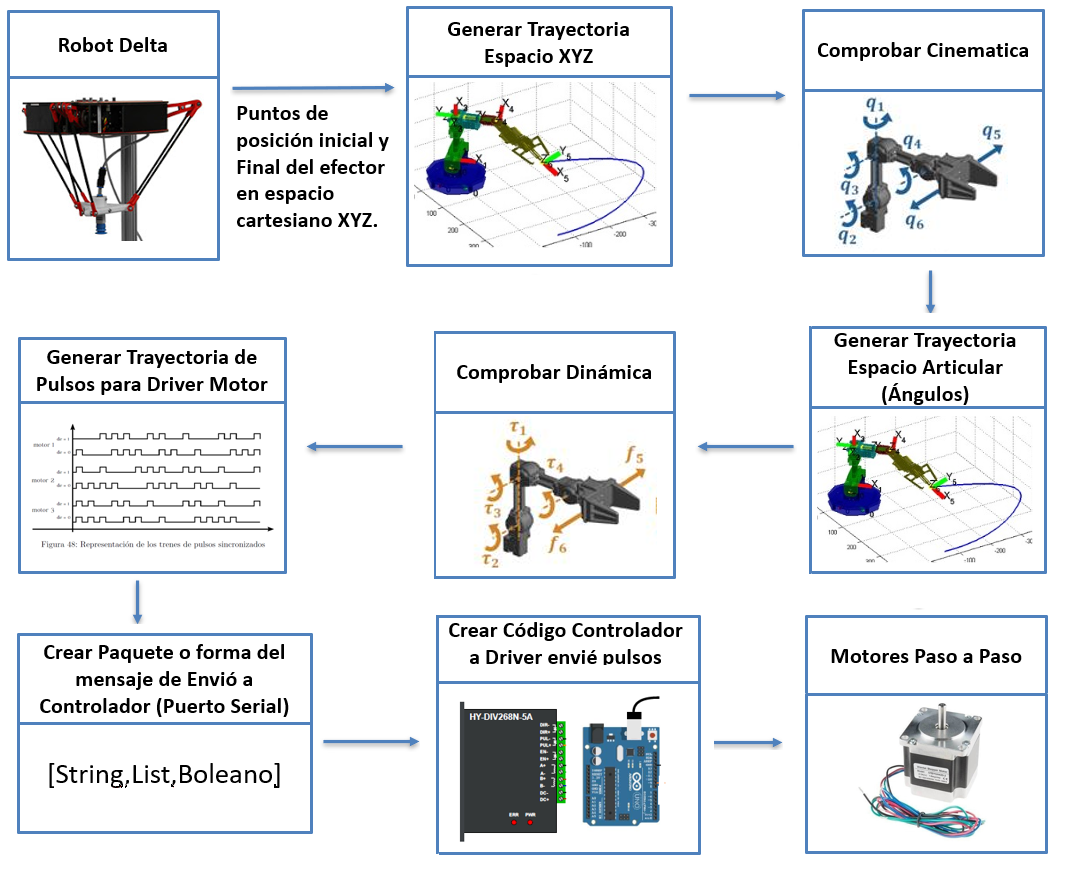
\includegraphics[width=1\linewidth]{Main/Chapter3/Images3/3-1/diagrama-de-flujo-robot.png}
        \caption{Ejemplo de diagrama de flujo de tareas que realiza un robot delta para realizar una trayectoria especifica}
        \label{f:Cap3-1_diagrama_de_flujo_robot_accion}
    \end{figure}
        \newpage
        
\section{Estructura de un robot delta}
%00X0 : reordenar los títulos del cap al diagrama de abajo en formato general, y luego explicar los software específicos para nosotros

    El robot delta puede ser subdivido por categorías de acuerdo al grupo estructural al que pertenezcan. Estas categorías facilitan la generación de conceptos para cada grupo de manera independiente, como se ilustra en la figura \eqref{f:Cap3-2_esquema_arquitectura_robot_delta}.
    
    \begin{figure}[h]
        \centering
        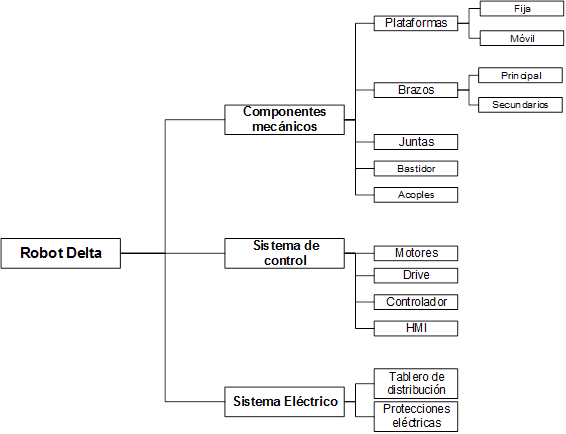
\includegraphics[width=0.85\linewidth]{Main/Chapter3/Images3/3-2/esquema-categorias-estructura.png}
        \caption{Descomposición estructural del robot delta \cite{Robot_parelelo_tipo}}
        \label{f:Cap3-2_esquema_arquitectura_robot_delta}
    \end{figure}
    
    \begin{enumerate}
        \item{ \textbf{Los componentes mecánicos}: son todas las piezas físicas que componen el robot delta. Es muy importante la elección del tipo de juntas a elegir ya que restringen el espacio de trabajo del robot delta. Por otro lado, se pueden optimizar las dimensiones de los largos de los brazos y antebrazos del robot con respecto a la energía suministrada a los motores y al espacio de trabajo.}
        \item{\textbf{El sistema de control}: es todo lo que está relacionado con el control del movimiento del robot delta. Los motores, que mueven los brazos del robot delta, deben controlarse a través de drivers por la complejidad de su accionamiento.}
        \item{ \textbf{El controlador}: puede tener el algoritmo que cree las trayectorias cartesianas para realizar el movimiento del robot de un punto a otro. El HMI es la interfaz que ayuda a visualizar si el movimiento deseado del robot es correcto antes de que se realice.}
        \item{   \textbf{Los componentes eléctricos}: son todo lo relacionado con la electricidad como fuentes de poder para los motores, cables de conexión, fusibles, switch, etc.}
    \end{enumerate}

        \newpage

    Con la intensión de modelar la arquitectura de un robot delta como guía para el desarrollo de este trabajo, se crea una arquitectura con ejemplos reales enfocado solo en el sistema de control, tal como se presenta en la figura \eqref{f:Cap3-2_esquema_sistema_control} donde:

    \begin{figure}[h]
        \centering
        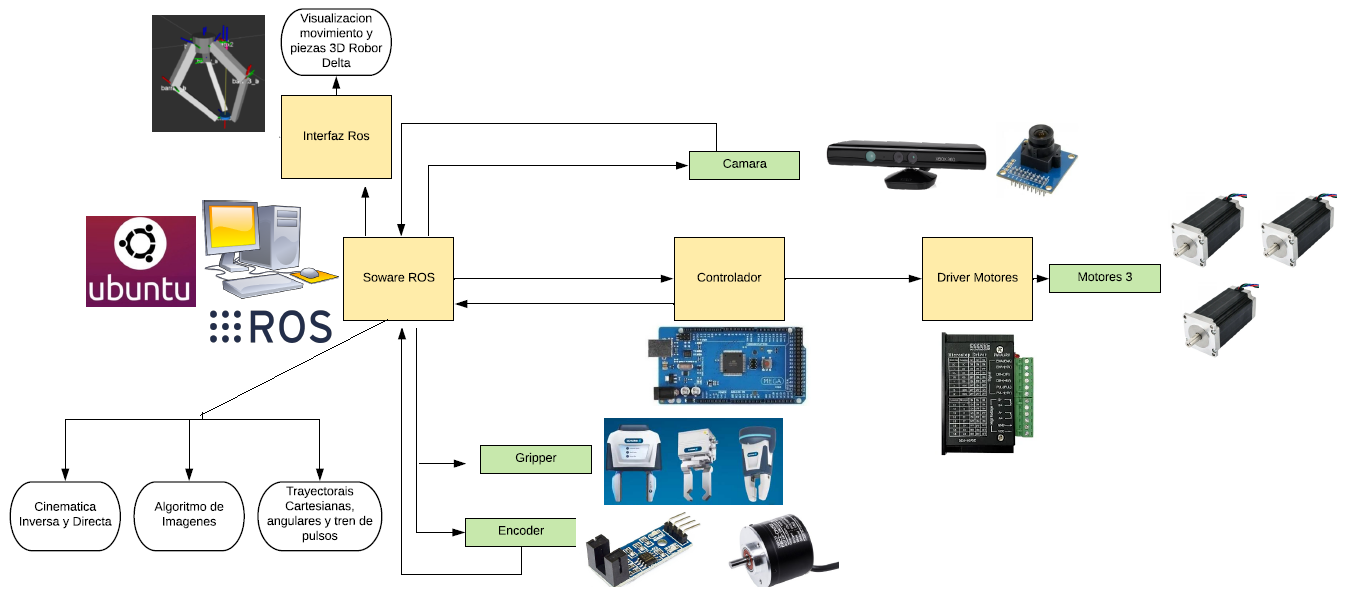
\includegraphics[width=1\linewidth]{Main/Chapter3/Images3/3-2/sistema-de-control.png}
        \caption{Ejemplo de el sistema de control de un robot delta}
        \label{f:Cap3-2_esquema_sistema_control}
    \end{figure}
    
    \begin{itemize}
        \item \textbf{Software ROS:} Es el encargado de procesar y ejecutar los algoritmos de cinemática y dinámica del robot delta. Además, controla el envió, la recepción y el procesamiento de datos de los sensores y el controlador.
        \item \textbf{Controlador:} Realiza la conversión de la trayectoria cartesiana o angular a un formato compatible con el driver de los motores. Se puede utilizar Arduino, Raspberry Pi, etc.
        \item \textbf{Rviz:} Es la interfaz gráfica que simula las trayectorias del robot.
        \item \textbf{Kinect:} Sensor RGB y de profundidad que controla la posición del robot creando un lazo cerrado.
        \item \textbf{Actuadores:} Motores paso a paso controlados por drivers.
        \item \textbf{Encoder:} Sensor de velocidad y posición angular que controla los actuadores creando un lazo cerrado.
        \item \textbf{Gripper:} Pinzas qe sujetan los objetos.
    \end{itemize}
    
    Para controlar a un alto nivel cada punto anterior, se necesita de mucho estudio, investigación y práctica, por lo que en esta tesis solo abarcara lo relacionado con el Software ROS y la interfaz gráfica Rviz.  
    
    \newpage

    
\section{Partes mecánicas}
    Con el fin de describir el robot delta, en esta sección se presenta un resumen del capítulo 2 de la tesis doctoral del ingeniero mecánico Reymond Clavel, el creador de este mecanismo, realizada en École Polytechnique Fédérale de Lausanne \cite{Clavel:31403}. 

    
    \subsection{Investigación}
    El primer objetivo que busca Reymond Clavel es el movimiento de piezas ligeras a gran velocidad en robots, ya que las aplicaciones objetivo de su investigación se encuentran en los campos del envasado en el sector alimentario, despaletización y paletización al inicio o al final de una línea de montaje, el montaje de componentes mecánicos, etc. Para todas estas operaciones se requiere un ritmo alto de producción/operación y los contactos de la industria de Clavel confirmaban esa tendencia en aquellos tiempos.
    
    Para lograr una alta tasa de trabajo durante operaciones que requieren carreras reducidas, el robot debe tener esencialmente una capacidad de aceleración y frenado; esta propiedad se obtiene mediante el uso de potentes actuadores debajo y mediante una estructura móvil muy ligera. Un estudio anterior de robot rápido del Clavel hizo posible probar el uso de gatos hidráulicos a alta velocidad con masas relativamente pesadas, pero por razones de coste y limpieza no querían utilizar energía hidráulica por lo que lo llevo al enfoque de una ``estructura móvil y ligera``.
    
    La búsqueda de un concepto se basó en una metodología enseñada en estudios de microtecnología en EPFL. Según la metodología antes mencionada, el primer paso de la cadena de costos consiste en definir la función global del producto considerado. La representación mediante una caja negra con las diferentes entradas y salidas sintetiza efectivamente esta información.
    
    \begin{figure}[htb]
        \centering
        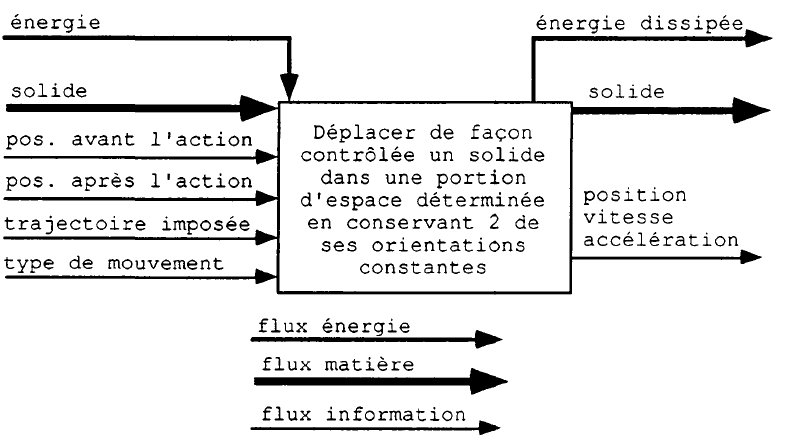
\includegraphics[width=0.75\linewidth]{Main/Chapter3/Images3/3-3/caja-negra-reymond.png}
        \caption{Representación de la función general del robot proyectada en forma de caja negra \cite{Clavel:31403}}
        \label{f:Cap3-3_caja_negra_reymond}
    \end{figure}
    
    \newpage
    
    \subsection{Elección del concepto ``Delta``}
    El catálogo de soluciones del anexo A2.2 de la tesis doctoral \cite{Clavel:31403} presenta 18 tipos de soluciones principales de la estructura de un robot delta que permiten mantener constantes 2 orientaciones de un sólido. La figura \eqref{f:Cap3-3_soluciones_interesantes_catalogo} muestra las soluciones más interesantes para el objetivo previsto. 

     \begin{figure}[htb]
        \centering
        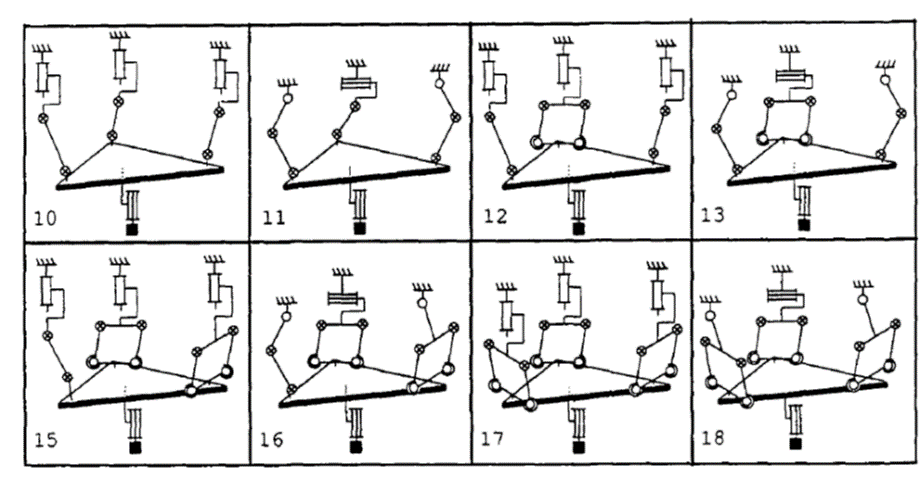
\includegraphics[width=0.85\linewidth]{Main/Chapter3/Images3/3-3/soluciones-interesantes.png}
        \caption{Extracto de las soluciones del catálogo del Apéndice A.2.2  \cite{Clavel:31403}}
        \label{f:Cap3-3_soluciones_interesantes_catalogo}
    \end{figure}
 
      \begin{figure}[htb]
        \centering
        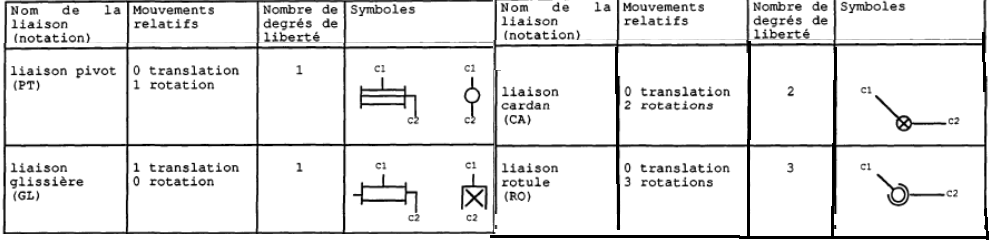
\includegraphics[width=0.8\linewidth]{Main/Chapter4/Images4/juntas.png}
        \caption{Nombre, movimiento relativo. grados de libertad y simbolos de juntas dibujadas en la figura  \eqref{f:Cap3-3_soluciones_interesantes_catalogo}  \cite{Clavel:31403}}
        \label{f:Cap3-3_soluciones_interesantes_catalogo_JUNTAS}
    \end{figure}
 
 Entre estas 18 soluciones, Reymond conserva aquellas que tienen las siguientes particularidades:   
    \begin{itemize}
        \item El movimiento en el espacio (con tres grados de libertad) es proporcionado por el tres actuadores asegurados a la base fija, las soluciones 10 a 13 y 15 a 18 de la figura \eqref{f:Cap3-3_soluciones_interesantes_catalogo} cumplen esta condición.
        \item Los actuadores son del tipo giratorio. Las soluciones 11, 13, 16 y 18 cumplen esta condicion.
        \item La estabilidad del órgano terminal está asegurada por una mayoría de elementos que trabajan en tensión-compresión más que en torsión. Finalmente se adopta la solución numero 18.
    \end{itemize}
    

    
        \newpage
    
    \subsection{Descripción del concepto ``Delta'' y sus componentes}
    La figura \eqref{f:Cap3-3_esquema_principal_robot_delta} sirve de apoyo para la descripción del robot Delta y su funcionamiento. Este es un robot con cuatro grados de libertad. Se compone principalmente de una ``base fija'' (1) integrada a un marco de soporte de la instalación y una placa móvil (5); el nombre que se le da a esta última pieza es ``góndola'' (nacelle en frances). La conexión entre la base fija (1) y la góndola (5) se realiza mediante tres cadenas cinemáticas, cada una de ellas está formado por un ``brazo'' (2) montado en una articulación pivotante sobre la base fija y 2 ``barras paralelas'' (3) provistas cada una de una articulación (4) en cada extremo. El conjunto anterior que forma 2 barras paralelas y 2 elementos de conexión al brazo y a la góndola, se denomina ``paralelogramo''. Cada brazo (2) es impulsado por un ``motor de brazo'' (7) que, con mayor frecuencia, adopta la forma de un conjunto de motor reductor de sensor. La ``Pinza'' (10) del motor (6), a través del ``eje telescópico'' (8) provisto de una articulación tipo cardan (9) tiene oculto uno de sus extremos.

    \vspace{-1em}

    % Multiples imagenes        
    \begin{figure}[h]
         \centering
              \subfloat[Esquema principal del robot delta]{
               \label{f:Cap3-3_esquema_principal_robot_delta}
                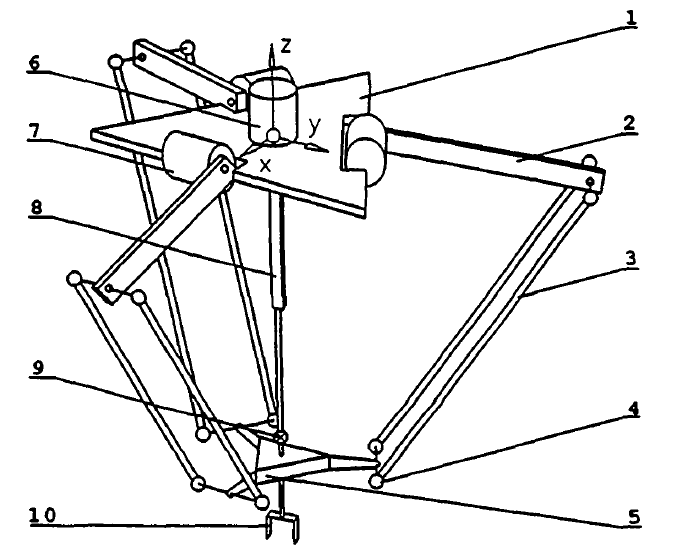
\includegraphics[width=0.5\textwidth]{Main/Chapter3/Images3/3-3/esquema-principal-robot-delta.png}}
              \subfloat[Representación de paralelogramos del robot delta]{
               \label{f:Cap3-3_ayuda_dimensiones}
                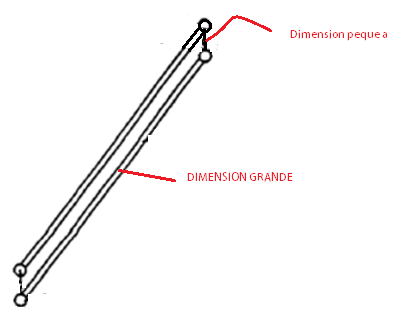
\includegraphics[width=0.5\textwidth]{Main/Chapter3/Images3/3-3/ayuda-dimensiones.png}}
         \caption{Descripción visual de un robot delta \cite{Clavel:31403}}
         %\label{f:animales}
    \end{figure}

    La orientación de la góndola está asegurada constantemente por los 3 paralelogramos (figura \eqref{f:Cap3-3_ayuda_dimensiones}), que comprenden cada uno 2 dimensiones pequeñas y 2 dimensiones grandes formadas por las barras paralelas. Cada lado pequeño integrado al extremo de un brazo permanece constantemente paralelo al eje de rotación del brazo en cuestión. Los 3 pares de barras paralelas aseguran que las 3 pequeñas dimensiones integradas a la góndola permanezcan paralelas a las pequeñas dimensiones integradas a los extremos de los brazos, por tanto, paralelas a los ejes de rotación de los brazos que, por construcción, se ubican en el mismo plano. Las juntas en los extremos de las barras paralelas son del tipo de junta esférica, por lo que cada barra puede girar alrededor de su eje longitudinal; esta rotación no altera el comportamiento de esta estructura articulada que forma el paralelogramo del espacio. Una conexión por resortes y estribos entre las 2 barras paralelas simplifica la construcción de las rótulas.
    
    \newpage

\section{Software Robor Operating System (ROS)}
    
        En esta sección se proporciona una descripción general de Robot Operating System, por sus siglas ROS y sus principales lineamientos. ROS es un marco para desarrollar software de robótica. El software está estructurado bajo un paradigma modular, pequeños paquetes que se comunican entre si mediante rápidos mensajes. Este paradigma se fomenta la reutilización de código y la colaboración global por sobre los entornos particulares.
    
    \begin{figure}[htb]
        \centering
        
\includegraphics[width=0.5\linewidth]{Main/Chapter3/Images3/3-4/logo-ros.png}
        \caption{Logo de ROS \cite{ros2222}}
        \label{f:Cap3-4_logo_ros}
    \end{figure}
    
    \subsection{Historia}
    
        ROS es un gran proyecto que tiene muchos antepasados y contribuyentes. Mucha gente en la comunidad de investigación robótica sintió la necesidad de un marco de colaboración abierto. Varios proyectos en la Universidad de Stanford (figura \eqref{f:Cap3-4_entidades_inicio_ros_32}) a mediados de la década de 2000 involucraban inteligencia artificial incorporada e integradora, como el Stanford AI Robot (STAIR) y el programa Personal Robots (PR), que crearon prototipos internos de los tipos de sistemas de software dinámicos y flexibles como lo es ROS. Se basó en Switchyard, que era parte de un proyecto de STAIR y fue escrito por Morgan Quigley en Stanford. En 2007, Willow Garage, Inc., una incubadora de robótica cercana, proporcionó importantes recursos para extender estos conceptos mucho más y crear implementaciones bien probadas. Desde el 2013 hasta el presente, ROS es mantenido permanentemente por Open Source Robotics Foundation (OSRF, figura \eqref{f:Cap3-4_entidades_inicio_ros_334}) de Google y desde el 2017 cambio su nombre a Open Robotics.
        
        \begin{figure}[htbp]
            \centering
            
\includegraphics[width=0.7\linewidth]{Main/Chapter3/Images3/3-4/entidade-asociadas-al-inicio-de-ros-3.png}
            \caption{OSRF \cite{osrf}} 
            \label{f:Cap3-4_entidades_inicio_ros_334}
        \end{figure}        
        
        \newpage
        
        La mayoría de las compañías y laboratorios de investigación en robótica están ahora portando su software a ROS. Esta tendencia también es visible en robots industriales, donde compañías están paulatinamente migrando de aplicaciones propietarias a ROS. El movimiento llamado ROS Industrial se ha incrementado en estos últimos años y su objetivo, básicamente, consiste en extender las capacidades avanzadas de ROS a la automatización y la robótica industrial. Este proyecto comenzó como un intento de colaboración de Yaskawa Motoman Robotics, Southwest Research Institute (SwRI) y Willow Garage (figura \eqref{f:Cap3-4_entidades_inicio_ros_33364}). En enero de 2012, Shaun Edwards de SwRI fundó un software repositorio, alojado en Github, donde la comunidad robótica puede encontrar interfaces para manipuladores industriales, pinzas, sensores y redes de dispositivos.
        
        \begin{figure}[htbp]
            \centering
            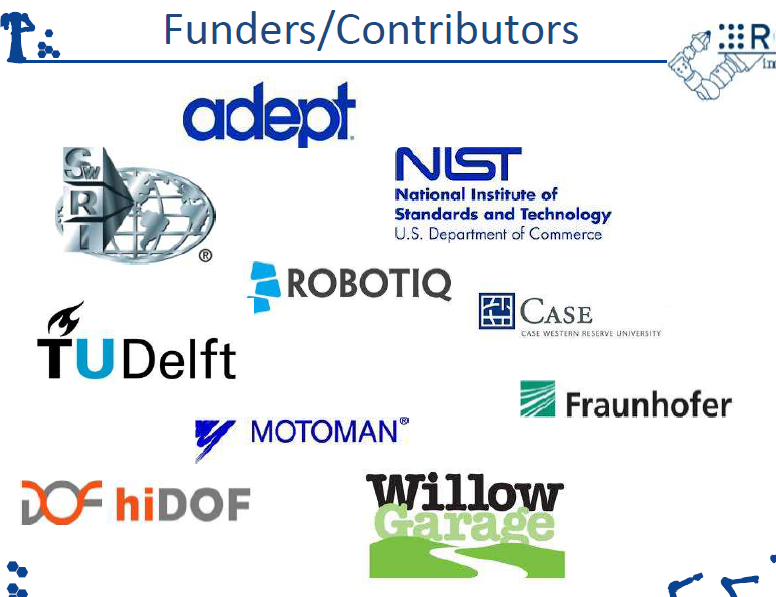
\includegraphics[width=0.65\linewidth]{Main/Chapter3/Images3/3-4/entidade-asociadas-al-inicio-de-ros-2.png}
            \caption{Fundadores y contribuidores de ROS} 
            \label{f:Cap3-4_entidades_inicio_ros_33364}
        \end{figure}    
        
        Finalizando con la breve historia de ROS, se puede decir que se utiliza en estos momentos en todo el mundo en instituciones académicas, industriales y de investigación. Los desarrolladores han contribuido con miles de paquetes, incluidas soluciones de algunos de los principales expertos del mundo en áreas específicas. Las nuevas empresas de robots ofrecen interfaces ROS con sus productos, y las empresas de robots industriales establecidas también están introduciendo interfaces ROS. Con la adopción generalizada de ROS como el enfoque estándar de factor para la programación de robots, existe una nueva esperanza de acelerar las capacidades de los robots.
        
        \begin{figure}[htbp]
            \centering
            
\includegraphics[width=0.6\linewidth]{Main/Chapter3/Images3/Stanford-University-logo1.jpg}
            \caption{Logo Stanford University \cite{stanford}} 
            \label{f:Cap3-4_entidades_inicio_ros_32}
        \end{figure}

    \newpage

    \subsection{Problema Principal}
    
    La intención con que se creó ROS fue de permitir a los investigadores desarrollar rápidamente nuevos sistemas robóticos sin tener que reinventar todo nuevamente, mediante el uso de herramientas e interfaces estándar. Para hacer más eficientes los procesos de investigación y desarrollo de software de robots, se detectaron los siguientes 3 problemas a solucionar:
    
    \begin{itemize}
        \item {Programación secuencial inadecuada para el mundo asincrónico robótico (figura \eqref{f:Cap3-4_entidades_ini_ros_1})}
        \item {Sistemas robóticos deben gestionar una complejidad significativa}
        \item {Abstracción de los detalles de un hardware específico del robot.}
    \end{itemize}

        \begin{figure}[htbp]
            \centering
            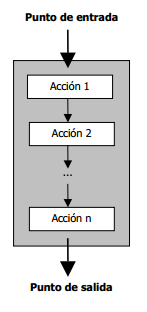
\includegraphics[width=0.25\linewidth]{Main/Chapter3/Images3/agrupar_problem_111.png}
            \caption{Programación Secuencial}
            \label{f:Cap3-4_entidades_ini_ros_1}
        \end{figure}
        
    La solución para el problema de programación secuencias se basó en Callback, que son una función que se ejecuta siempre que hay datos disponibles para su procesamiento. Son asincrónico, ya que la devolución de llamada puede ocurrir en cualquier momento. Con respecto a el problema de softwares multifuncionales complejos y atracción de detalles de hardware específicos, se separaron los procesos en “nodos” que se comunican a través de una interfaz de mensajería. Por ejemplo, se separaron los procesos de las cámaras, edometría, escáner láser y creación de mapas y estos interactúan a través de una interfaz que comunica estos procesos por medio de “temas”. Estos últimos conceptos se explican en detalle en secciones posteriores.

    \newpage


    \subsection{Que es ROS}
       ROS es una abreviatura de  Robot Operating System y es una plataforma de desarrollo de aplicaciones en robótica que provee estilos de programación (en particular, que se basa en nodos distribuidos y acoplados libremente); definiciones de interfaz y paradigmas para las comunicaciones entre nodos ; definiciones de interfaz para la incorporación de bibliotecas y paquetes; una colección de herramientas para visualización, depuración, registro de datos y diagnóstico del sistema; un repositorio de código fuente compartido; y puentes a múltiples bibliotecas útiles e independientes de código abierto.
       
       El objetivo principal de ROS es apoyar la reutilización de código en la investigación y el desarrollo de robótica. ROS es un marco distribuido de procesos (también conocido como nodos) que permite que los ejecutables se diseñen individualmente y se acoplen libremente en tiempo de ejecución. Estos procesos se pueden agrupar en paquetes, que se pueden compartir y distribuir fácilmente. ROS también es compatible con un sistema federado de repositorios de código que también permite la distribución de la colaboración. Este diseño, desde el nivel del sistema de archivos hasta el nivel de la comunidad, permite decisiones independientes sobre el desarrollo y la implementación, pero todos pueden combinarse con las herramientas de infraestructura ROS.
       
       ROS no es un sistema operativo convencional como Windows, Linux y Android en el sentido tradicional de gestión y programación de procesos; más bien, es un meta-sistema operativo que se ejecuta en el sistema operativo. Las diferencias entre un OS y ROS se muestran el la figura \eqref{f:Cap3-4_diferencias_ros_so}. ROS es un middleware, que proporciona los servicios que esperaría de un sistema operativo, incluida la abstracción de hardware, control de dispositivos de bajo nivel, implementación de funciones de uso común, transmisión de mensajes entre procesos y administración de paquetes. También proporciona herramientas y bibliotecas para obtener, compilar, escribir y ejecutar código en varios equipos.
       
        \begin{figure}[htb]
            \centering
            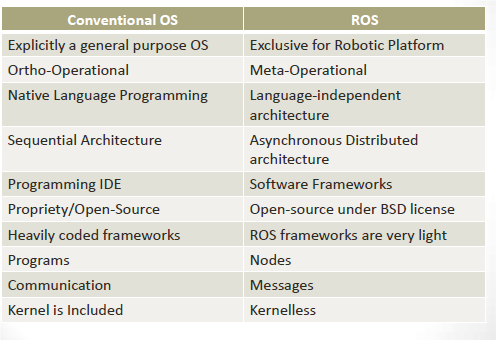
\includegraphics[width=0.65\linewidth]{Main/Chapter3/Images3/3-4/diferencia-ROS-SO.png}
            \caption{Diferencias entre un sistema operativo convencional y ROS}
            \label{f:Cap3-4_diferencias_ros_so}
        \end{figure}
        
        \newpage
        
        Las principales características de ROS se pueden resumir de la siguiente manera:
        
        \begin{itemize}
            \item \textbf{Plumbing:} ROS proporciona una infraestructura de mensajería de publicación y suscripción diseñada para respaldar la construcción rápida y sencilla de sistemas informáticos distribuidos.
            \item \textbf{Herramientas} ROS proporciona un amplio conjunto de herramientas para configurar, iniciar, introspectar, depurar, visualizar, registrar, probar y detener sistemas informáticos distribuidos.
            \item \textbf{Capacidades} ROS proporciona una amplia colección de bibliotecas que implementan funcionalidades robóticas útiles, con un enfoque en la movilidad, la manipulación y la percepción.
            \item \textbf{Ecosistema:} ROS es apoyado y mejorado por una gran comunidad, con un fuerte enfoque en la integración y documentación. ros.org es una ventanilla única que busca y aprende sobre los miles de paquetes ROS que están disponibles a través de desarrolladores de todo el mundo.
        \end{itemize}

        Un ejemplo se muestra en la figura \eqref{f:Cap3-4_compatibilidad_ros}, la comunicación de datos ROS es compatible no solo con un sistema operativo, sino también con múltiples sistemas operativos, hardware y programas, lo que lo hace muy adecuado para el desarrollo de robots donde se combinan varios hardware. 
        
        \begin{figure}[htb]
            \centering
            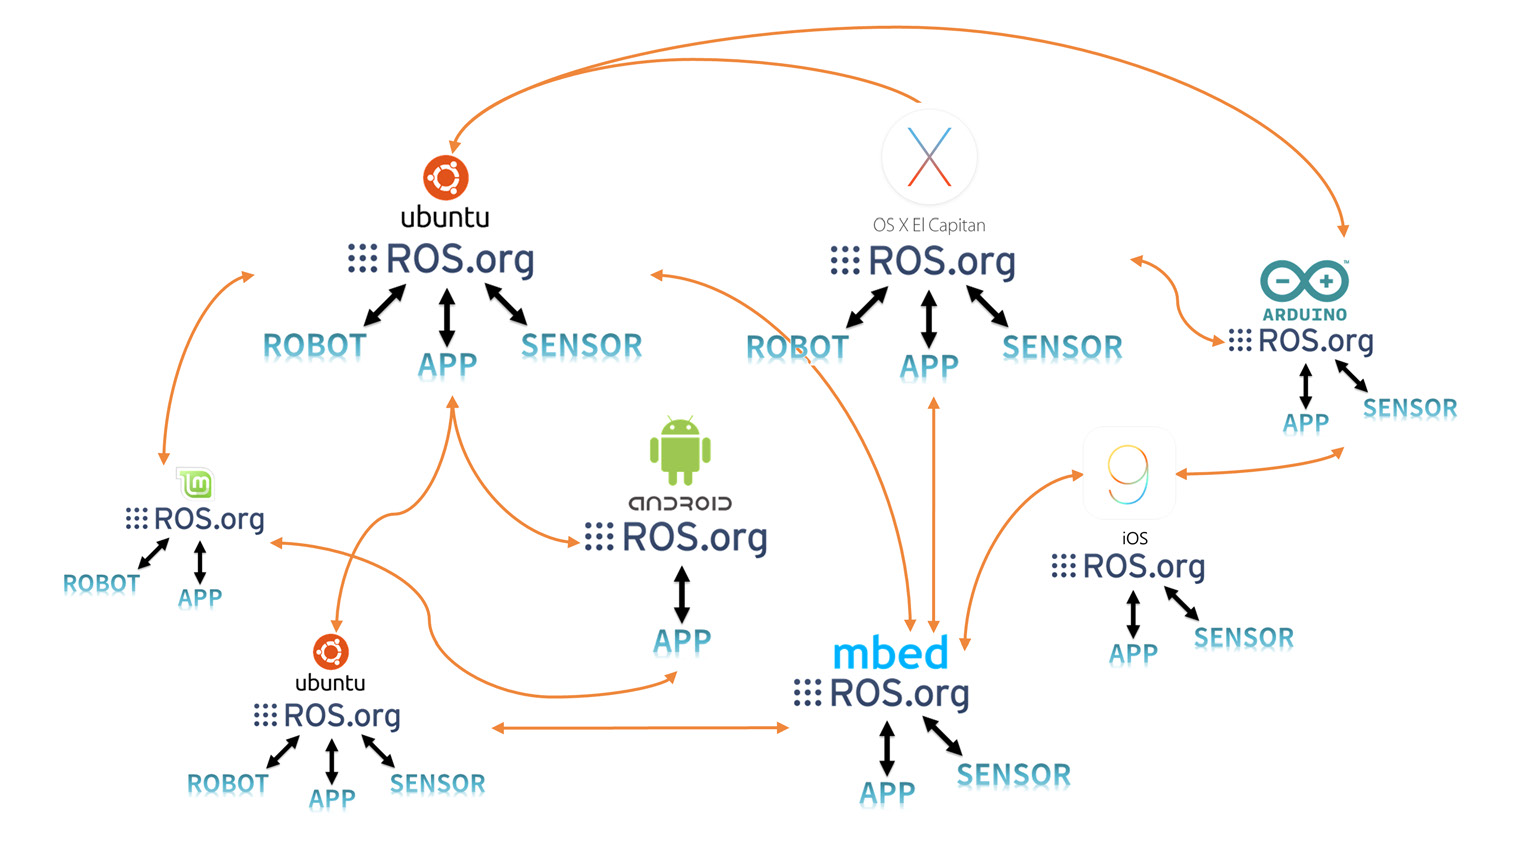
\includegraphics[width=1.0\linewidth]{Main/Chapter3/Images3/3-4/compatibilidad-ros.png}
            \caption{Compatibilidad de ROS y otras plataformas \cite{ROS_BOOK_1}}
            \label{f:Cap3-4_compatibilidad_ros}
        \end{figure}
        
    \newpage

        
    \subsection{Objetivos de ROS}
    
        Todos los marcos de software imponen sus filosofías de desarrollo a sus colaboradores directa o indirectamente, a través de sus modismos y prácticas comunes. En términos generales, ROS sigue la filosofía de desarrollo de software de Unix en varios aspectos clave. Esto tiende a hacer que ROS se sienta ``natural'' para los desarrolladores que provienen de Unix, pero algo ``críptico'' al principio para aquellos que han utilizado principalmente entornos de desarrollo gráfico en Windows o Mac OS X. Los siguientes párrafos describen varios aspectos filosóficos de ROS.
        
        \subsubsection{Peer to peer (Nodos)}
        
            Los sistemas ROS consisten en numerosos programas pequeños de computadora que se conectan entre sí e intercambian mensajes continuamente. Estos mensajes viajan directamente de un programa a otro; no hay un servicio de enrutamiento central. Aunque esto hace que la ``plumbing'' subyacente sea más compleja, el resultado es un sistema que escala mejor a medida que aumenta la cantidad de datos. La mentalidad Peer to peer se representa en la figura \eqref{f:Cap3-5_arquitectura_ros}.
            
            \begin{figure}[htb]
                \centering
                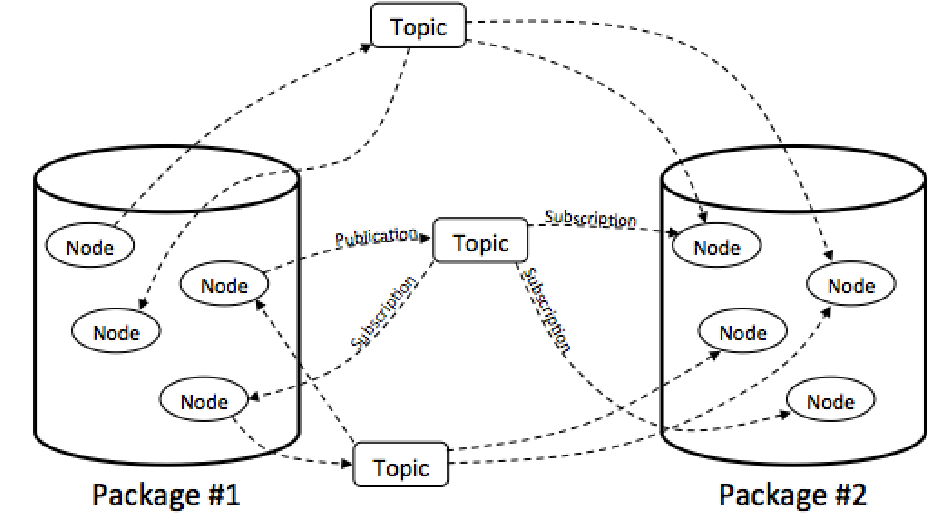
\includegraphics[width=0.8\linewidth]{Main/Chapter3/Images3/arquitectura_por_nodos_1.png}
                \caption{Modelo de cómo los nodos ROS publican y se suscriben a temas \cite{naval_delta}}
                \label{f:Cap3-5_arquitectura_ros}
            \end{figure}
            
        \subsubsection{Orientación hacia las herramientas}
        
            Como lo demuestra la arquitectura duradera de Unix, se pueden crear sistemas de software complejos a partir de muchos programas pequeños y genéricos. A diferencia de muchos otros marcos de software de robótica, ROS no tiene un entorno de ejecución y desarrollo integrado canónico. Tareas como navegar por el árbol del código fuente, visualizar las interconexiones del sistema, trazar gráficamente los flujos de datos, generar documentación, registrar datos, etc, son todas realizadas por programas separados. Esto fomenta la creación de implementaciones nuevas y mejoradas, ya que (idealmente) se pueden intercambiar por implementaciones más adecuadas para un dominio de tarea en particular. Las versiones recientes de ROS permiten que muchas de estas herramientas se compongan en procesos únicos para mayor eficiencia o para crear interfaces coherentes para operadores o depuración, pero el principio sigue siendo el mismo: las herramientas individuales en sí mismas son relativamente pequeñas y genéricas.
            
        \subsubsection{Multilenguaje}
        
            Muchas tareas de software son más fáciles de realizar en lenguajes de secuencias de comandos de ''alta productividad'' como Python o Ruby. Sin embargo, hay ocasiones en las que los requisitos de rendimiento exigen el uso de lenguajes más rápidos, como C ++. También hay varias razones por las que algunos programadores prefieren lenguajes como Lisp o MATLAB. Se han librado guerras interminables de correo electrónico, se están librando actualmente y, sin duda, se seguirá librando sobre qué idioma es el más adecuado para una tarea en particular. Reconociendo que todas estas opiniones tienen mérito, que los lenguajes tienen diferentes utilidades en diferentes contextos, y que la experiencia única de cada programador es muy importante al elegir un idioma, ROS eligió un enfoque multilingüe. Los módulos de software ROS se pueden escribir en cualquier idioma para el que se haya escrito una biblioteca cliente. En el momento de escribir este artículo, existen bibliotecas cliente para C ++, Python, LISP, Java, JavaScript, MATLAB, Ruby, Haskell, R, Julia y otros. Las bibliotecas de cliente ROS se comunican entre sí siguiendo una convención que describe cómo los mensajes se ``aplanan'' o ``serializan'' antes de transmitirse a través de la red. La figura \eqref{f:Cap3-5_multilenguaje_ros} representa un ejemplo de multilenguaje en ROS. En ella se muestra el nodo ''Laser Scanner'' escrito en lenguaje Python con el objetivo de obtener datos de un entorno físico por medio de un escáner de láser y el nodo ''Map Building'' escrito en lenguaje C++ encargado de transformar los datos obtenidos por del nodo anterior para poder visualizarlos a la computadora.     
            
            \begin{figure}[htb]
                \centering
                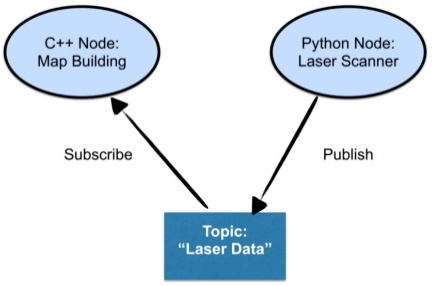
\includegraphics[width=0.5\linewidth]{Main/Chapter3/Images3/multilenguaje_1.png}
                \caption{Ejemplo de multilenguaje de ROS}
                \label{f:Cap3-5_multilenguaje_ros}
            \end{figure}

\newpage
            
        \subsubsection{Pequeño}
        
            Las convenciones ROS alientan a los contribuyentes a crear bibliotecas independientes y luego empaquetar esas bibliotecas para que puedan enviar y recibir mensajes hacia y desde otros módulos ROS. Esta capa adicional está destinada a permitir la reutilización de software fuera de ROS para otras aplicaciones, y simplifica en gran medida la creación de pruebas automatizadas utilizando herramientas de integración continua estándar.
            
        \subsubsection{Libre y Open Source}
        
            El núcleo de ROS se publica bajo la licencia BSD permisiva, que permite el uso comercial y no comercial. ROS pas datos entre módulos mediante comunicación entre procesos (IPC), lo que significa que los sistemas construidos con ROS pueden tener licencias detalladas de sus diversos componentes. Los sistemas comerciales, por ejemplo, a menudo tienen varios módulos de fuente cerrada que se comunican con una gran cantidad de módulos de fuente abierta. Los proyectos académicos y de pasatiempos suelen ser de código abierto. El desarrollo de productos comerciales a menudo se realiza completamente detrás de un firewall. Todos estos casos de uso, y más, son comunes y perfectamente válidos bajo la licencia ROS.
            
            \begin{figure}[htb]
                \centering
                
\includegraphics[width=0.3\linewidth]{Main/Chapter3/Images3/3-5/licnecia-bsd-ros.png}
                \caption{Licencia de ROS}
                \label{f:Cap3-5_multilenguaje_ros}
            \end{figure}
            

\newpage

    \subsection{Estadisticas}
    
    \subsubsection{Science Robotics}
        Science Robotics publico el articulo el 2017 “Powering the world’s robots 10 years of ROS” \cite{Zhangeaar1868} que habla sobre la iniciativa ROS-I (Ros Industrial) que se lanzó en 2012. Debido a las arquitecturas de software limitadas de los robots industriales actuales, es demasiado caro aplicar capacidades robóticas avanzadas para mejorar la productividad industrial. ROS-I proporciona interfaces para robots industriales comunes y dispositivos sensoriales junto con bibliotecas de software específicas para la automatización de la fabricación. ROS-I ha apoyado un número creciente de hardware industrial, como los robots producidos por ABB, Fanuc y Yaskawa. Además, el Consorcio ROS-I existe para desarrollar la comunidad ROS-I proporcionando apoyo técnico, organizando cursos de capacitación y talleres, y estableciendo la hoja de ruta para ROS-I. El Consorcio ROS-I tiene más de 50 miembros en todo el mundo, incluidos institutos de investigación y agencias gubernamentales, integradores de sistemas y usuarios finales, y fabricantes de equipos originales. Además, la próxima versión de ROS 2.0 debería abordar una de las principales limitaciones que ha ralentizado la adopción de ROS en la industria: que es una implementación de middleware interna. ROS 2.0 ahora se basa en el servicio de distribución de datos para la comunicación entre procesos, lo que brinda una confiabilidad mucho mejor con protocolos de calidad de servicio y seguridad con cifrado.

        La figura \eqref{f:Cap3-5_estadisticas_1} muestra algunas estadísticas clave de ROS, las cuales son:

            \begin{figure}[htb]
                \centering
                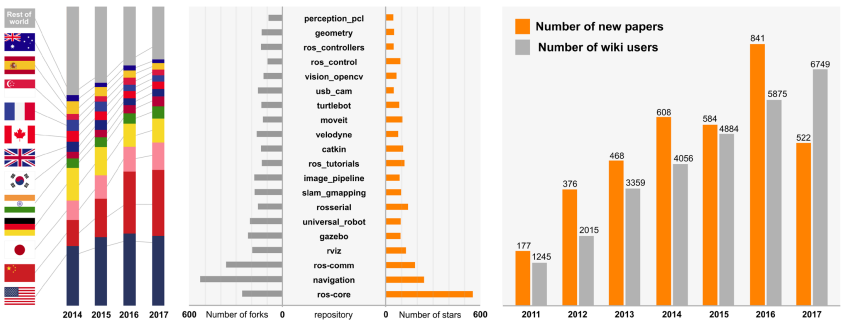
\includegraphics[width=1.0\linewidth]{Main/Chapter3/Images3/science_robot_esta_1.png}
                \caption{Estadísticas mundiales de ROS \cite{Zhangeaar1868}}
                \label{f:Cap3-5_estadisticas_1}
            \end{figure}        

        \begin{itemize}
            \item {Los países visitantes de la wiki de ROS en los últimos 4 años, muestra un cambio creciente de investigadores de países del Lejano Oriente (información recolectada del informe métrico anual de ROS). }
            \item {Los 20 principales repositorios ROS según la cantidad de bifurcaciones y estrellas (de Github, 10 de octubre de 2017).}
            \item {Artículos recientemente publicados en los últimos 10 años que han citado el artículo ''ROS original'' (de la búsqueda de Google Scholar, palabras clave “Sistema operativo de robot ROS”) y el número de usuarios de wiki registrados.}
        \end{itemize}
        

        La figura \eqref{f:Cap3-5_estadisticas_2} muestra los diez años de desarrollos de ROS que respaldan la investigación y el desarrollo, incluida la robótica móvil, industrial, quirúrgica y espacial, así como los automóviles autónomos. Se han lanzado 11 distribuciones de ROS en los últimos 10 años, y el gráfico de barras muestra el número de descargas binarias de ROS en cada año. El Consorcio ROS-I se lanzó en 2013 con el objetivo de transformar las capacidades de ROS en tiempo real para robots industriales. ROS 2.0 es actualmente en desarrollo intenso, y se acaba de lanzar una versión beta.

            \begin{figure}[htb]
                \centering
                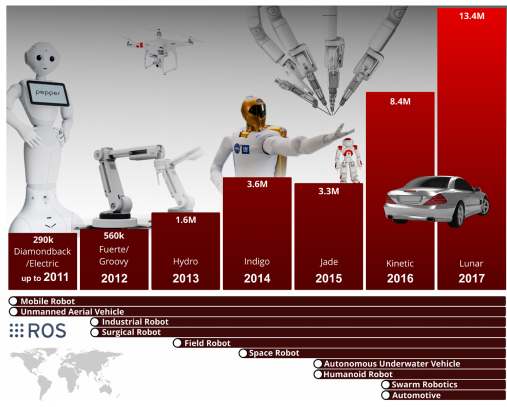
\includegraphics[width=1.0\linewidth]{Main/Chapter3/Images3/science_robot_esta_2.png}
                \caption{Desarrollo de ROS en los últimos 10 años \cite{Zhangeaar1868}}
                \label{f:Cap3-5_estadisticas_2}
            \end{figure}  


         \newpage
    
        \subsubsection{Metricas de la comunidad ROS}
    
    Ros Metrics miden aspectos de la comunidad ROS para comprender y rastrear el impacto de su trabajo e identificar áreas de mejora. Se inspiran en las métricas del Proyecto MeeGo .
    
        \begin{figure}[htb]
            \centering
            
\includegraphics[width=0.4\linewidth]{Main/Chapter3/Images3/cap3_estadisticas_3.png}
            \caption{Logo de ROS Metrics \cite{rosmetrics}}
            \label{f:Cap3-5_estadisticas_3}
        \end{figure}  
        
        Las figuras \eqref{f:Cap3-5_estadisticas_4} y \eqref{f:Cap3-5_estadisticas_5} presentan estadísticas recolectadas de la pagina oficial de ROS Metrics hasta el año 2021. Según la figura \eqref{f:Cap3-5_estadisticas_4}, los países que más han visitado ROS son China, EEUU, Japón y Alemania. 
        
        \begin{figure}[htb]
            \centering
            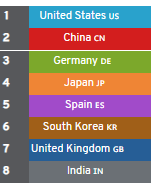
\includegraphics[width=0.27\linewidth]{Main/Chapter3/Images3/cap3_estadisticas_7.png}
            \caption{Top de países que utilizan ROS en base a la descarga de paquetes registrados hasta el 28 de marzo del año 2021 \cite{rosmetrics}.}
            \label{f:Cap3-5_estadisticas_4}
        \end{figure}  
        

        \begin{figure}[htb]
            \centering
            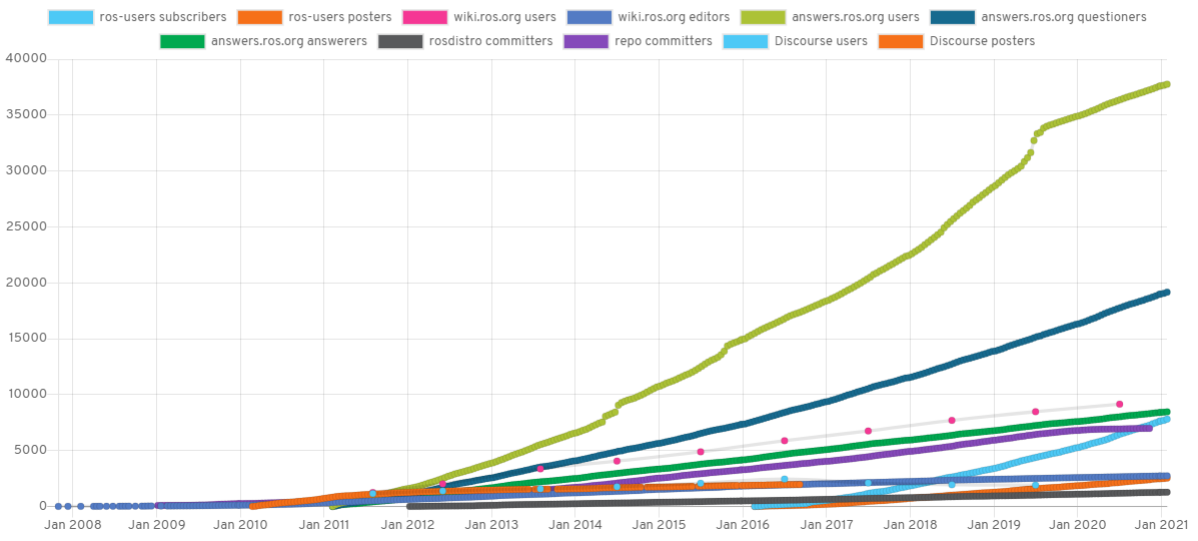
\includegraphics[width=1.0\linewidth]{Main/Chapter3/Images3/cap3_estadisticas_4.png}
            \caption{Colección de diferentes métricas para medir la cantidad de usuarios de la comunidad ROS \cite{rosmetrics}}
            \label{f:Cap3-5_estadisticas_5}
        \end{figure}  
        
        \newpage

        \subsubsection{Repositorio GitHub}
            Para comprender GitHub, primero se debe comprender Git. Git es un sistema de control de versiones de código abierto que fue iniciado por Linus Torvalds, la misma persona que creó Linux. Sirve para cuando los desarrolladores crean algo (una aplicación, por ejemplo), realizan cambios constantes en el código, lanzando nuevas versiones hasta y después del primer lanzamiento oficial. Los sistemas de control de versiones mantienen estas revisiones en orden, almacenando las modificaciones en un repositorio central. Esto permite a los desarrolladores colaborar fácilmente, ya que pueden descargar una nueva versión del software, realizar cambios y cargar la revisión más reciente. Todos los desarrolladores pueden ver estos nuevos cambios, descargarlos y contribuir. Del mismo modo, las personas que no tienen nada que ver con el desarrollo de un proyecto aún pueden descargar los archivos y usarlos. Git es una herramienta de línea de comandos, pero el centro alrededor del cual giran todas las cosas relacionadas con Git es el centro, GitHub.com, donde los desarrolladores almacenan sus proyectos y se conectan con personas de ideas afines.
    
            \begin{figure}[htb]
            \centering
            
\includegraphics[width=0.23\linewidth]{Main/Chapter3/Images3/repo_git_1.png}
            \caption{Logo GitHub, Inc.}
            \label{f:Cap3-5_estadisticas_8}
            \end{figure} 
        
            Dirk Thomas trabajo en ROS durante casi 9 años y envio 15 distribuciones de ROS. Uno del repositorio que subió a GitHub registra el total de autores, commits y repositorios en Github con relación a ROS hasta octubre del 2020.
        
            \begin{figure}[htb]
            \centering
            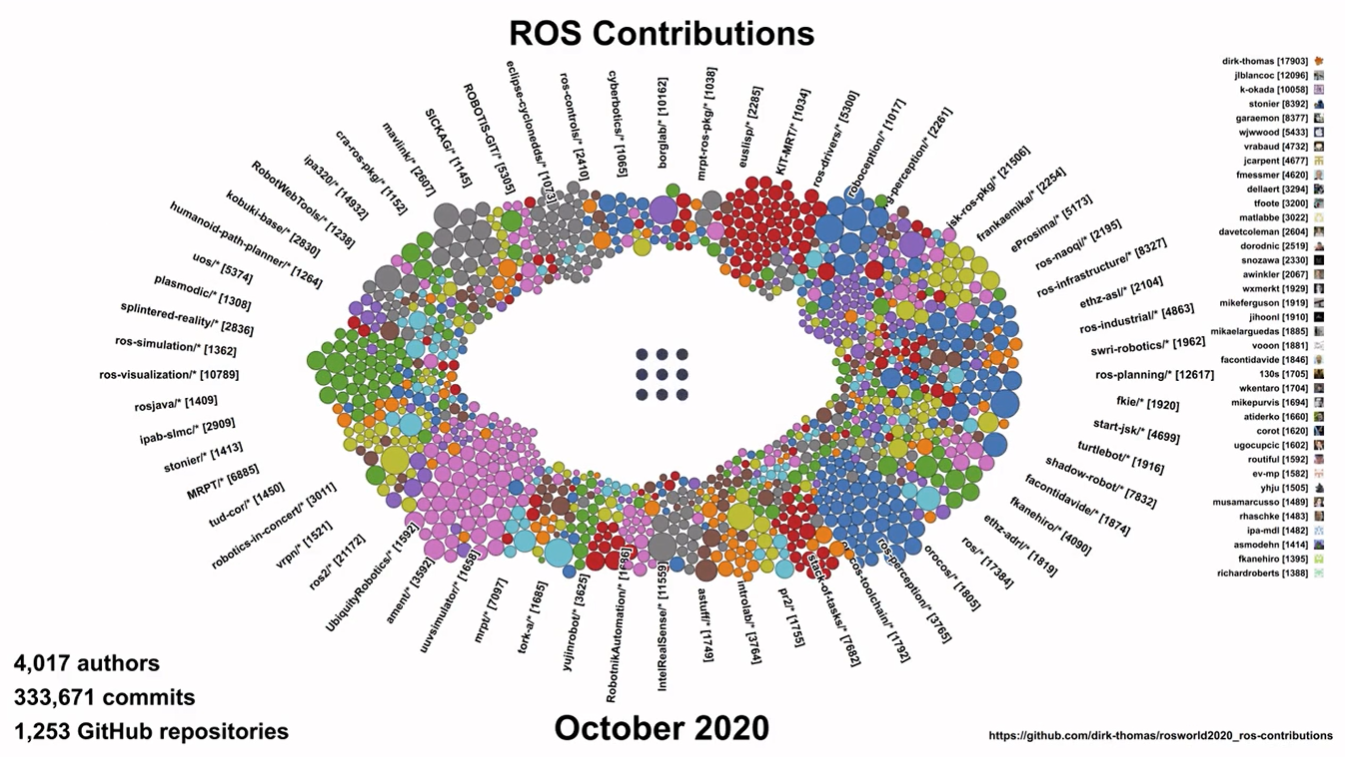
\includegraphics[width=0.99\linewidth]{Main/Chapter3/Images3/repo_git_2.png}
            \caption{Visualización de las contribuciones de ROS en GitHub \cite{gitreposito}}
            \label{f:Cap3-5_estadisticas_9}
            \end{figure} 
    
        \newpage

    \subsection{Versiones}
            En 2007, Willow Garage logró la investigación del marco de software de robot que comenzó en el laboratorio de inteligencia artificial de la Universidad de Stanford y continuó el desarrollo bajo el nombre de Robot Operating System. Con la sexta versión de lanzamiento oficial "ROS Groovy Galápagos", Willow Garage intentó penetrar en el mercado de robots de servicios comerciales en 2013, pero terminó dividiéndose en varias empresas emergentes y finalmente se entregó a la Open Source Robotics Foundation. Desde entonces, se lanzaron 4 versiones más y, a partir de mayo de 2017, OSRF cambió su nombre a Open Robotics y ha estado desarrollando, operando y administrando ROS. Más recientemente, la undécima versión de ROS, ROS Lunar Loggerhead, fue lanzada el 23 de mayo de 2017. ROS etiqueta la primera letra de cada nombre de lanzamiento en orden alfabético y usa una tortuga como su símbolo (ver figura \eqref{f:Cap3-5_estadisticas_10}).
            
            \begin{figure}[htb]
            \centering
            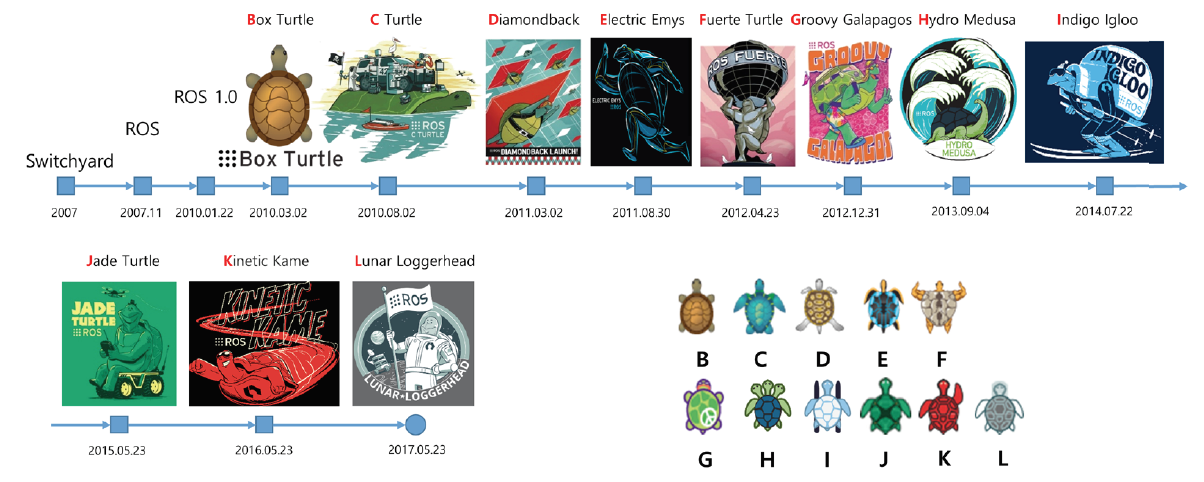
\includegraphics[width=0.94\linewidth]{Main/Chapter3/Images3/ver_ros_1.png}
            \caption{Linea temporal e iconos de tortuga para cada versión de ROS \cite{ROS_BOOK_1}}
            \label{f:Cap3-5_estadisticas_10}
            \end{figure} 
    
            \begin{figure}[htb]
            \centering
            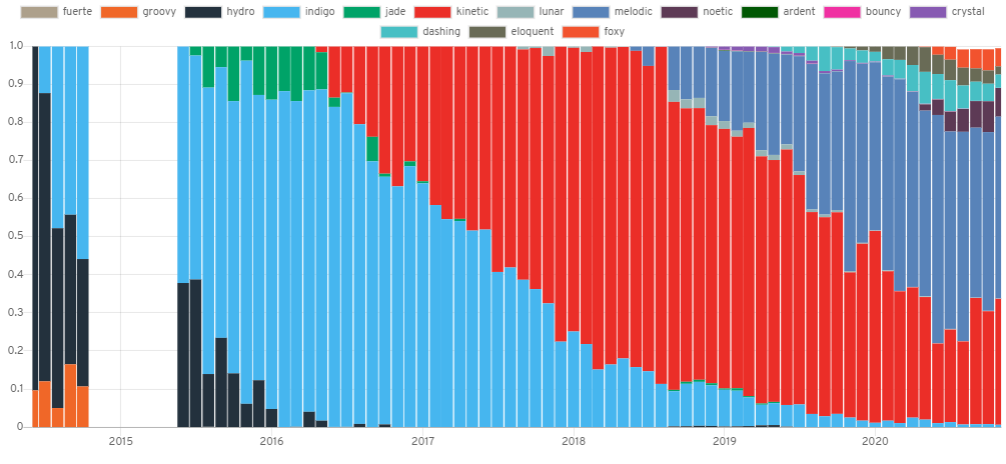
\includegraphics[width=0.94\linewidth]{Main/Chapter3/Images3/ver_ros_2.png}
            \caption{Uso relativo de cada versión de ROS basado en descargas de packages.ros.org \cite{rosmetrics}.}            \label{f:Cap3-5_estadisticas_11}
            \end{figure} 
    
    \newpage
    
    \subsection{Conceptos principales}
            
            Hay tres niveles de conceptos en ROS. El primero se refiere a cómo diferentes archivos están organizados en la computadora, herramientas ROS para administrar código fuente, instrucciones de compilación y definiciones de mensajes (nivel de sistema de archivos). El segundo son los componentes de la red peer to peer de nodos ROS, es decir, los procesos. (nivel de gráfico computacional). Por último, el nivel 3 es en relación a cómo los usuarios comparten software para permitir que todos lo utilicen (nivel comunitario).
            
            \begin{figure}[htb]
                \centering
                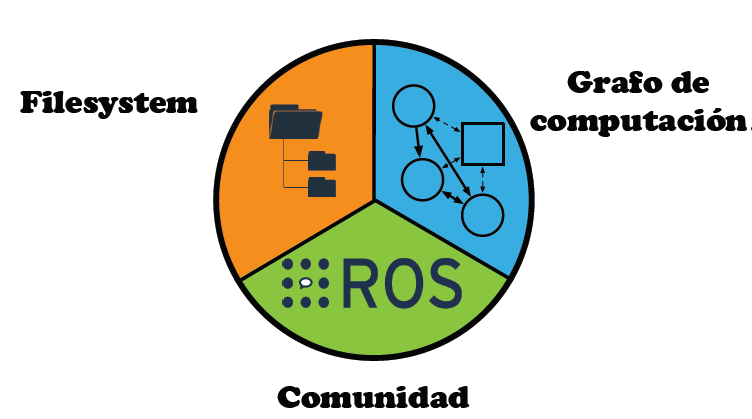
\includegraphics[width=1\linewidth]{Main/Chapter3/Images3/nivel_s_a_1.png}
                \caption{Niveles de conceptos de ROS}
                \label{f:Cap3_conceptos_1}
            \end{figure} 
            

                
                
               \newpage
               
            \subsubsection{Nivel de sistemas de archivos}

                Similar a un sistema operativo, los archivos de ROS también se organizan en el disco duro de una manera particular. En este nivel, se puede ver cómo se organizan estos archivos en el disco. La figura \eqref{f:Cap3_conceptos_2} muestra cómo se organizan los archivos y carpetas:
                
                
            \begin{figure}[htb]
                \centering
                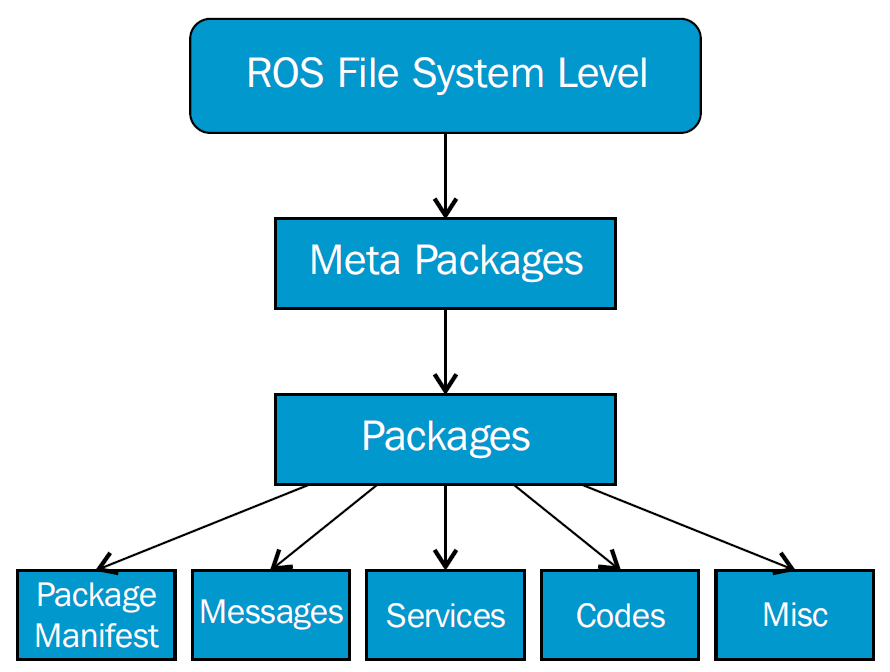
\includegraphics[width=0.55\linewidth]{Main/Chapter3/Images3/n_s_a_2.png}
                \caption{Nivel de sistema de archivos ROS \cite{lentin_2015}}
                \label{f:Cap3_conceptos_2}
            \end{figure} 
                
                

            A cuntinuacion se presenta la descripcion de cada bloque en el sistema de archivos:
            \begin{itemize}
                \item {\textbf{Meta packages:} Es un único paquete lógico compuesto por muchos paquetes en su interior. Además, los meta paquetes contienen un archivo package.xml que describe la carpeta y sus dependencias.}
                \item {\textbf{Packages:} Son las unidades más bajas y la principal para organizar el software en ROS. Un paquete puede contener procesos en tiempo de ejecución ROS (nodos), un Biblioteca dependiente de ROS, conjuntos de datos, archivos de configuración o achivos de lanzamiento. Cada directorio de paquete debe incluir un archivo CMakeList.txt y package.xml que describa el contenido del paquete y cómo catkin debe interactuar con él.}
                \item {\textbf{Stacks:} Son grupos de paquetes que se juntan para realizar funciones de alto nivel.}
                \item {\textbf{Manifests:} Los manifiestos proporcionan metadatos sobre un paquete. Pueden pertenecer a un packages o una Stacks y describen información general sobre un paquete o Stacks específico, como una breve descripción de lo que hace, el nombre del autor, su tipo de licencia y las dependencias.con otros paquetes.}
                \item {\textbf{Message (msg) types:} Las descripciones de los mensajes definen los datos estructuras para mensajes enviados en ROS.}
                \item {\textbf{Service (srv) types:} Las descripciones de servicio definen la solicitud y estructuras de datos de respuesta para servicios en ROS.}
            \end{itemize}
            
               \newpage
               
            ROS está basado en CMake y puede ser utilizado por muchos sistemas operativos como Linux o Windows. CMake es un generador de herramientas de creación, una herramienta de nivel superior, que simplifica el proceso de compilación y construcción, puede gestionar grandes proyectos y tiene una buena escalabilidad. Para una plataforma a gran escala como ROS, se usa CMake, y ROS ha extendido CMake, por lo que hay un sistema de compilación Catkin. Catkin es el sistema de compilación de ROS que genera programas ejecutables, bibliotecas e interfaces y proporciona el concepto de espacio de trabajo en la construcción de cada proyecto.
            
            La estructura del espacio de trabajo catkin, incluye las carpetas src, build, devel. Las tres rutas también pueden incluir otras en algunas opciones de compilación. Pero estas tres carpetas son las predeterminadas para el sistema de compilación catkin. Sus roles específicos son los siguientes:

            \begin{itemize}
                \item {\textbf{Espacio fuente (src):} Contiene el código fuente donde el usuario puede extraer, verificar o clonar el código fuente de los paquetes que quiere construir.}
                \item {\textbf{Espacio de construcción (build):} Este es el espacio donde CMake apela para construir los paquetes en el espacio de trabajo de catkin. CMake y Catkin mantienen su información de caché y otros intermedios archivos.}
                \item {\textbf{Espacio de desarrollo (devel):} Se encuentran archivos de objetos generados (incluidos archivos de encabezado, bibliotecas de vínculos dinámicos, bibliotecas de vínculos estáticos, archivos ejecutables, etc.), variables de entorno}
            \end{itemize}


            Durante el proceso de compilación, el flujo de trabajo de un catkin workspace es el que se muestra con flechas azules en la figura \eqref{f:Cap3_conceptos_3}. Los dos últimos procesos son generados y administrados automáticamente por el sistema catkin. El uso principal para los usuarios de ROS es la carpeta src\/, donde los paquetes creados o copiados se almacenan en dicha carpeta. En el momento de la compilación, el sistema de compilación de catkin busca y compila todos los paquetes de código fuente de forma de src\/.

            \begin{figure}[htb]
                \centering
                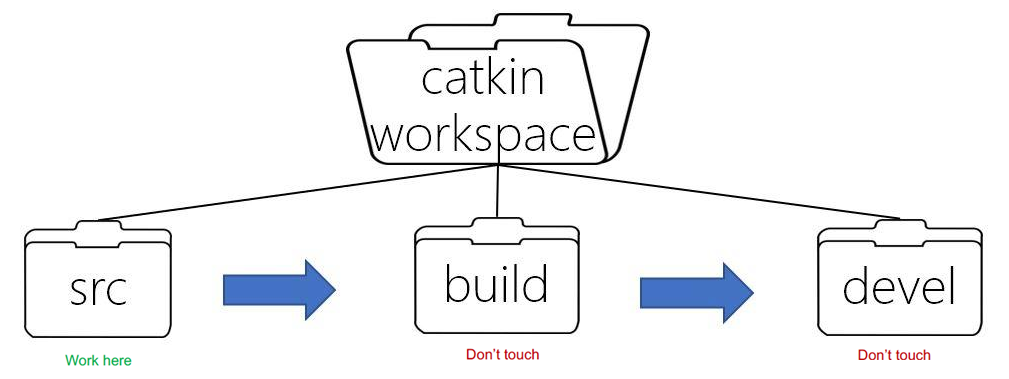
\includegraphics[width=0.8\linewidth]{Main/Chapter3/Images3/n_s_a_3.png}
                \caption{Espacio de trabajo catkin\_make \cite{cmake_blogcsdn}}
                \label{f:Cap3_conceptos_3}
            \end{figure} 
            
               \newpage


            Cuando se crea un paquete, normalmente es común encontrar las carpetas de la figura \eqref{f:Cap3_conceptos_4} dentro de el:
            
            \begin{figure}[htb]
                \centering
                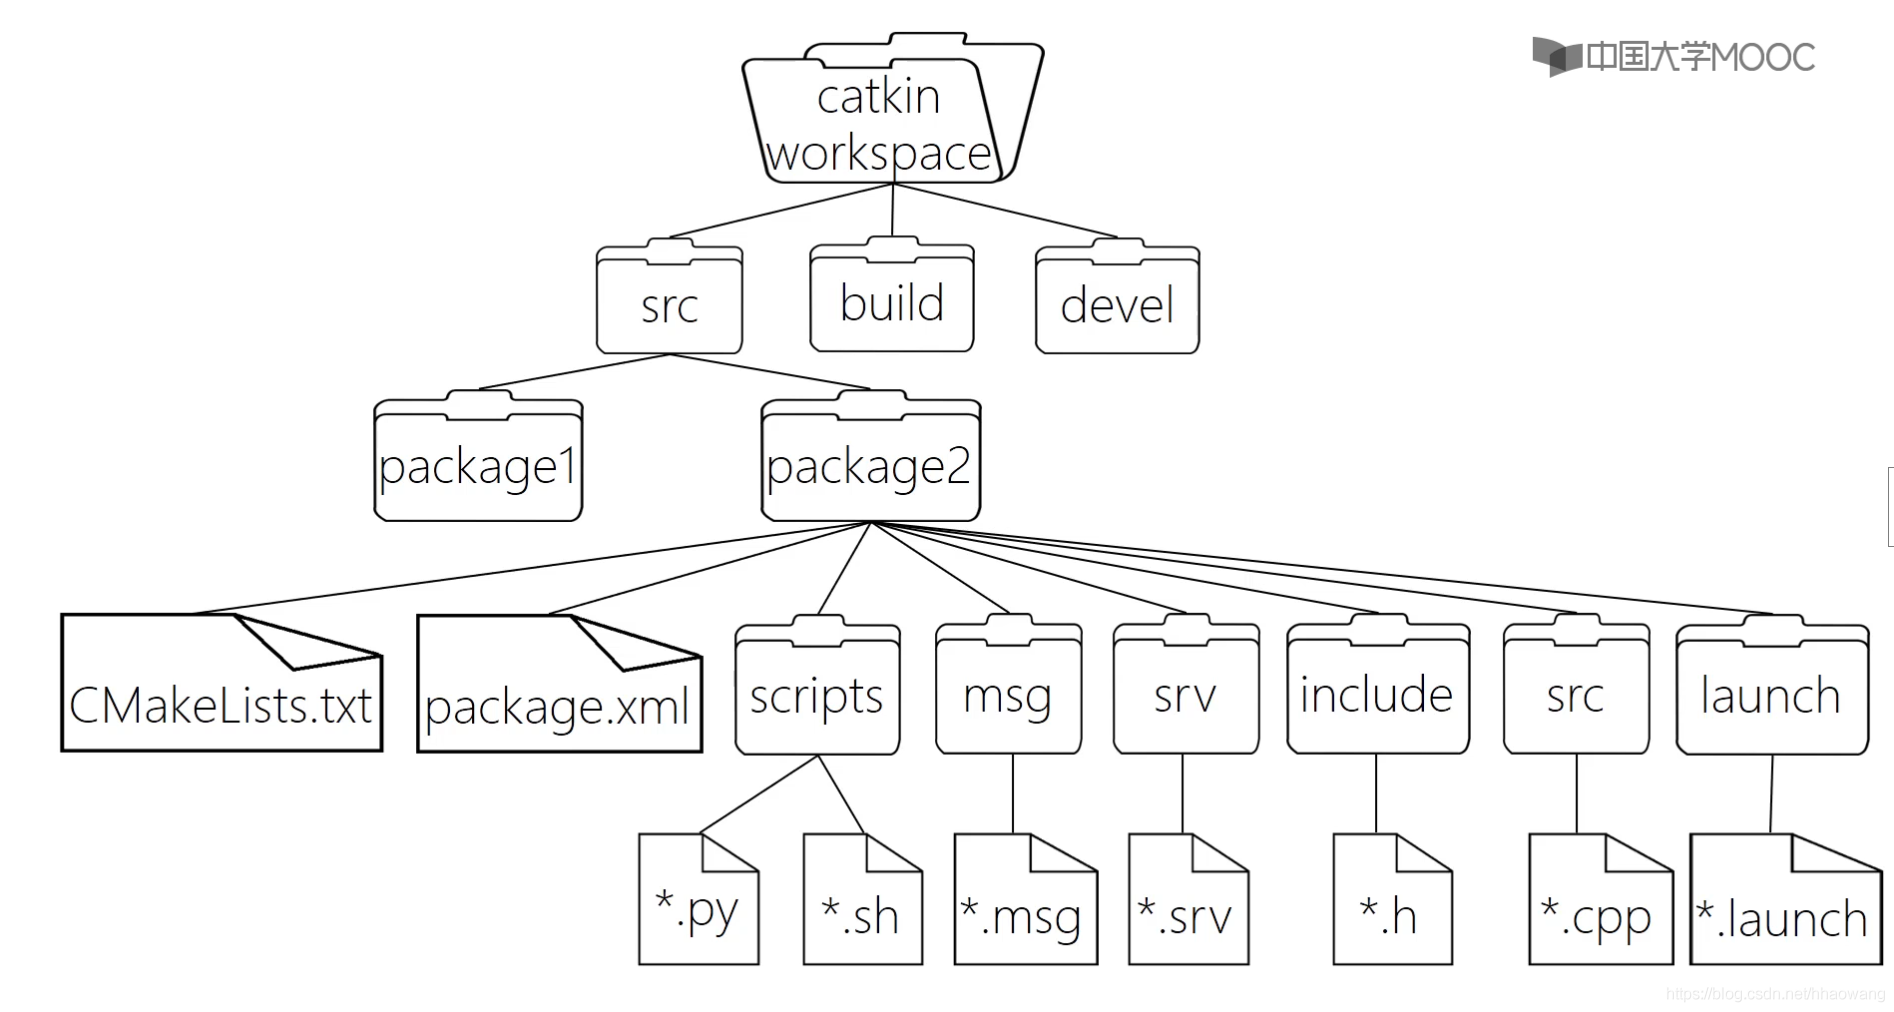
\includegraphics[width=1.0\linewidth]{Main/Chapter3/Images3/n_s_a_4.png}
                \caption{Estructura y características de catkin\_make \cite{cmake_blogcsdn}}
                \label{f:Cap3_conceptos_4}
            \end{figure} 

            \begin{itemize}
                \item {\textbf{/include/:} Esta carpeta contiene los encabezados (*.h) y las bibliotecas (*.lib, *.so).}
                \item {\textbf{/config/:} Todas las configuraciones se almacenan en esta carpeta incluidos los parámetros definidos, como controlador de robot con una extensión (*.yaml).}
                \item {\textbf{/launch/:} Contiene los archivos (*.launch) para ejecutar los nodos seleccionados del paquete o de otros paquetes usando el comando <incluir/>.}
                \item {\textbf{/msg/:} Contiene el tipo de datos del mensaje para nuestra aplicación (*.msg).}
                \item {\textbf{/srv/:} Esta carpeta contiene el tipo de mensaje para los servicios (*.srv).}
                \item {\textbf{/actions/:} Contiene el tipo de datos del mensaje utilizado en las acciones (*.action). }
                \item {\textbf{/src/:} Todo el código que se va a computar en el paquete debe estar dentro de esta carpeta con extensión (*.cpp).}
                \item {\textbf{package.xml:} Descripción del paquete y lista de dependencias utilizadas por el.}
                \item {\textbf{CmakeLists.txt:} Lista de requisitos y dependencias que debe compilar el ejecutador del paquete.}
            \end{itemize}

\newpage
            \subsubsection{Nivel gráfico computacional}
            
            El nivel gráfico computacional describe la infraestructura que utilizan los componentes ROS para comunicarse. Se basa en una red de procesos peer-to-peer (nodos) y se compone de varias unidades tales como las de la figura \eqref{f:Cap3_conceptos_5}:
            
            \begin{figure}[htb]
                \centering
                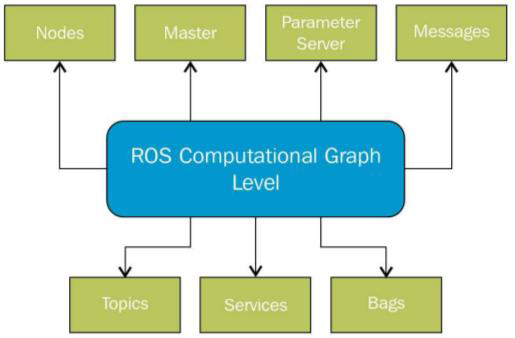
\includegraphics[width=0.63\linewidth]{Main/Chapter3/Images3/n_s_a_5.png}
                \caption{Estructura de la capa ROS Graph \cite{lentin_2015}}
                \label{f:Cap3_conceptos_5}
            \end{figure} 
            
            \paragraph{Nodes (Nodos)}
                   Son ejecutables en el sistema ROS y realizan la parte computacional. Se pueden conectar a otros nodos mediante 2 tipos de comunicación: Publisher/Subscriber o Services. Cada nodo tiene su propio nombre para ser reconocido y distinguido de los demás nodos. En ROS existen muchos lenguajes para programar un nodo como C ++, Python o Java. 
                   
            \paragraph{Ros Master}
                    Ros Master habilita el funcionamiento de la red ROS y es el primer proceso que debe ejecutarse cuando estamos usando ROS. Su función es registrar todos los nodos que se ejecutan y los temas y servicios existentes. Esto es esencial para interconectar nodos y monitorear todas las unidades en el sistema
            \begin{figure}[htb]
                \centering
                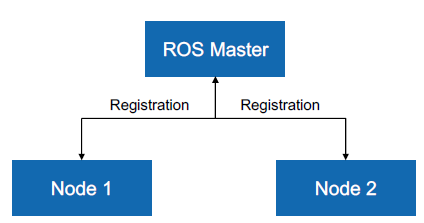
\includegraphics[width=0.55\linewidth]{Main/Chapter3/Images3/n_s_a_6.png}
                \caption{Registro de nodos en ROS Master \cite{rosmaster_diagram}.}
                \label{f:Cap3_conceptos_6}
            \end{figure} 
            
            
               \newpage


            \paragraph{Topics (Temas)}
                Los nodos comparten información pasando y recibiendo mensajes. Estos mensajes se publican con un nombre especial llamado tema. Por lo tanto, los nodos pueden publicar o suscribirse a un tema específico para obtener los mensajes deseados. Muchos nodos se pueden suscribir al mismo tema para recibir los mensajes que necesitan. Las comunicaciones entre nodos se realizan de forma unidireccional, por lo que cualquier nodo que envíe la información sobre un tema no puede recibir respuesta en el mismo canal, ni saber si el nodo receptor ha recibido el mensaje.
            \begin{figure}[htb]
                \centering
                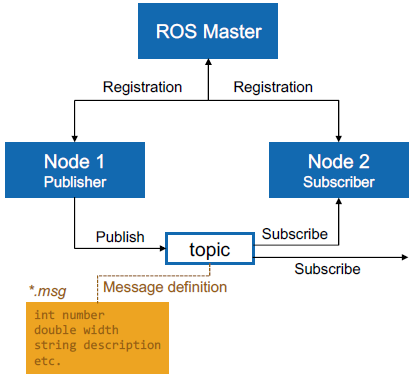
\includegraphics[width=0.68\linewidth]{Main/Chapter3/Images3/n_s_a_7.png}
                \caption{Nodos comunicándose a través de topic por medio de un mensaje *.msg \cite{rosmaster_diagram}.}
                \label{f:Cap3_conceptos_7}
            \end{figure} 
            \begin{figure}[htb]
                \centering
                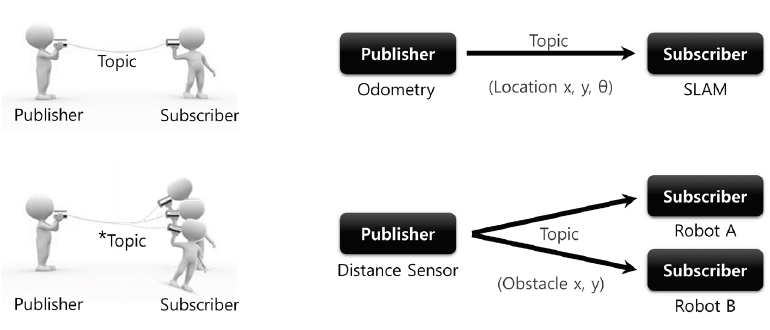
\includegraphics[width=0.92\linewidth]{Main/Chapter3/Images3/n_s_a_8.PNG}
                \caption{Comunicación de mensajes por medio de topics \cite{ROS_BOOK_1}}
                \label{f:Cap3_conceptos_8}
            \end{figure} 


               \newpage


            \paragraph{Services (Servicios)}
                 Aunque el principal método de comunicación entre nodos es a través de temas, ya que explicado anteriormente, existe otra metodología en ROS llamada llamadas de servicio. Las llamadas de servicio ROS son diferentes de mensajes debido a las siguientes características: son bidireccionales y uno a uno. 
                 
                Este proceso síncrono de comunicación se basa en un sistema cliente / servidor o solicitud / respuesta., donde un nodo cliente envía algunos datos llamados solicitud a un nodo servidor y espera hasta que el servidor pueda responder. Los servidor, habiendo recibido esta solicitud, toma alguna acción  y enviar algunos datos llamados respuesta al nodo cliente
                La descripción del servicio se almacena en un archivo de definición de servicio *.msg, guardado en un subdirectorio /srv. 

            \begin{figure}[htb]
                \centering
                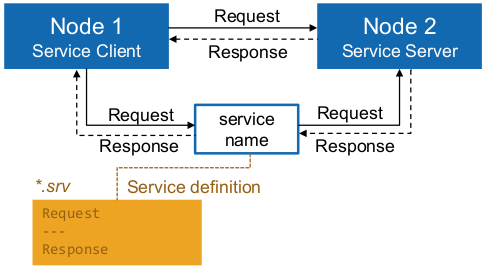
\includegraphics[width=0.85\linewidth]{Main/Chapter3/Images3/n_s_a_9.png}
                \caption{Comunicación request/response entre nodos que realizan servicios \cite{rosmaster_diagram}.}
                \label{f:Cap3_conceptos_9}
            \end{figure} 
            
            \begin{figure}[htb]
                \centering
                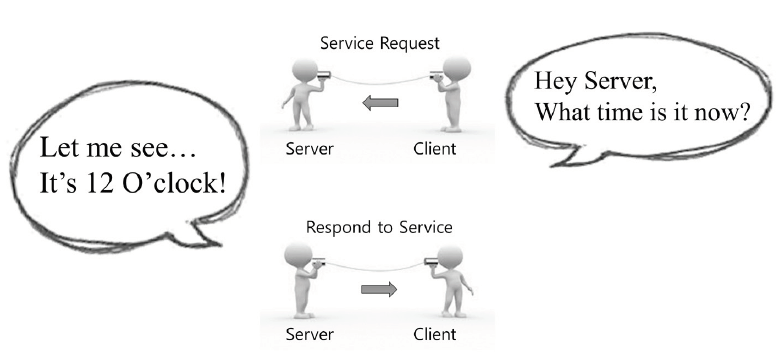
\includegraphics[width=1.0\linewidth]{Main/Chapter3/Images3/n_s_a_10.PNG}
                \caption{Comunicación de mensajes de servicio \cite{ROS_BOOK_1}.}
                \label{f:Cap3_conceptos_10}
            \end{figure}             

               \newpage

            \paragraph{ Actions (Acciones)}
                    Una acción es una comunicación bidireccional asíncrona entre los nodos activos basados en el cliente de la acción y el sistema del servidor de la acción que se muestra en la figura \eqref{f:Cap3_conceptos_11}. El sistema de acción, como los servicios explicados anteriormente, envía algo del cliente de acción de datos al servidor de acción llamado objetivo y el servidor de acción responde un resultado. Las acciones se diferencian de los servicios porque el servidor puede proporcionar retroalimentación y estado al cliente en cualquier momento sobre el proceso que se está realizando y el nodo cliente puede cancelar el objetivo anterior requerido para el servidor en cualquier momento también.
                    Al igual que en las llamadas de servicio ROS, las acciones deben definir pocos mensajes para comunicar al cliente con el servidor. Esto es posible gracias a las especificaciones de acciones, que definen estos mensajes en un archivo de acción con extensión *.action. Estos archivos generalmente se almacenan en una subcarpeta /action/ en el directorio del paquete.
                    El archivo * .action se divide en 3 secciones. Cada parte está separada por 3 guiones (---). En la primera parte se define el objetivo, en la segunda se establece la retroalimentación y en la última se especifica la definición del resultado.

            \begin{figure}[htb]
                \centering
                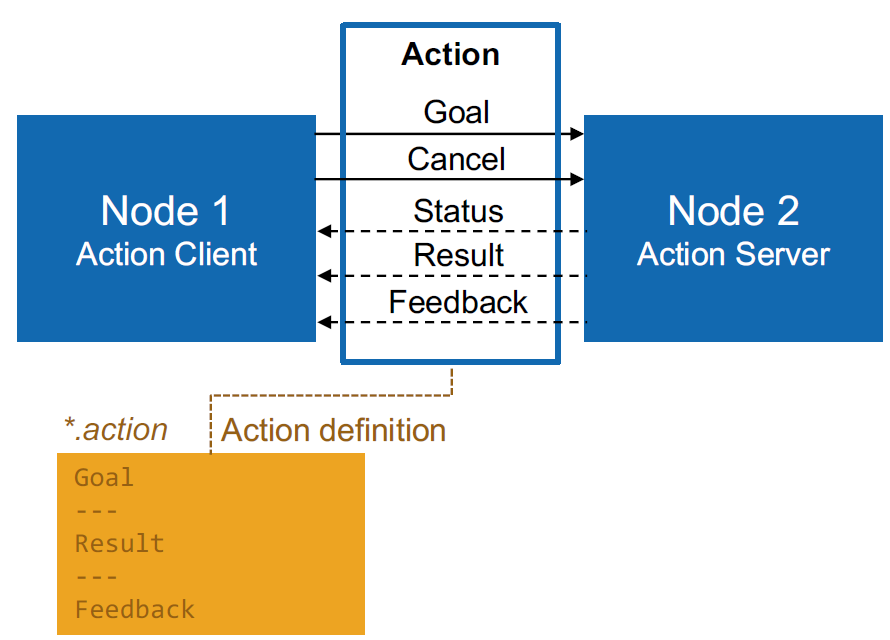
\includegraphics[width=0.7\linewidth]{Main/Chapter3/Images3/action_diagram.png}
                \caption{Comunicación bidireccional entre nodos por medio de acciones \cite{rosmaster_diagram}.}
                \label{f:Cap3_conceptos_11}
            \end{figure}             

            \begin{figure}[htb]
                \centering
                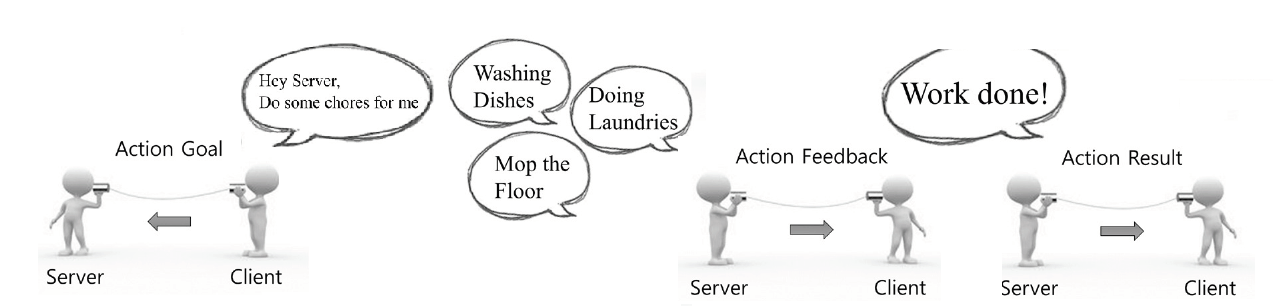
\includegraphics[width=1.0\linewidth]{Main/Chapter3/Images3/n_s_a_12.png}
                \caption{Comunicación de mensajes de acción \cite{ROS_BOOK_1}.}
                \label{f:Cap3_conceptos_12}
            \end{figure}   

               \newpage

            \paragraph{Messages (Mensajes)}
                Un mensaje es simplemente una estructura de datos, que comprende campos escritos. Tipos primitivos estándar (entero, punto flotante, booleano, etc.) son compatibles (figura \eqref{f:Cap3_conceptos_13}). En muchos paquetes utilizados en ROS se incluyen mensajes especiales llamados 'encabezado', que son básicamente mensajes creados por otros. Hay tres campos definidos en un mensaje de encabezado: 
                
                \begin{itemize}
                    \item {\textbf{uint32 seq:} Corresponde al número del mensaje enviado por un editor determinado}
                    \item {\textbf{time stamp: } La hora exacta a la que se envió el mensaje}
                    \item {\textbf{string frame\_id:} Muestra el sistema de referencia utilizado}
                \end{itemize}

            \begin{figure}[htb]
                \centering
                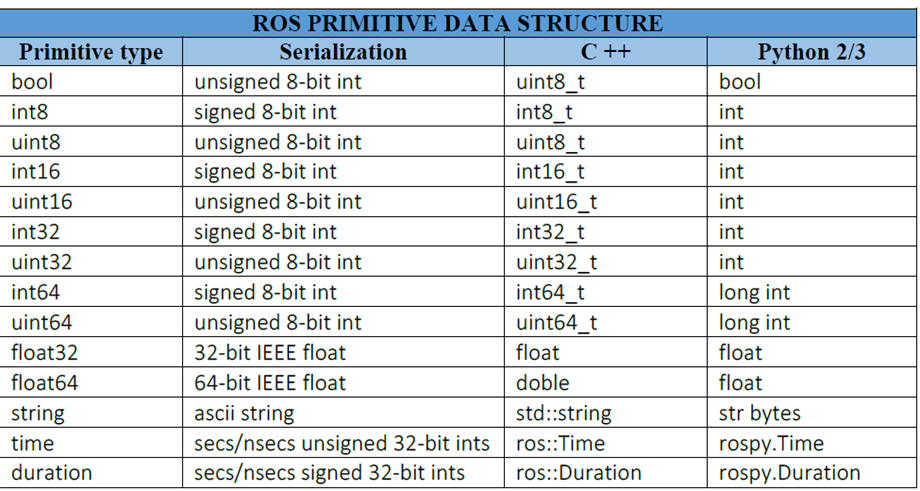
\includegraphics[width=1.0\linewidth]{Main/Chapter3/Images3/n_s_a_13.png}
                \caption{Tipos de datos basicos para mensajes en ROS \cite{ROS_BOOK_1}.}
                \label{f:Cap3_conceptos_13}
            \end{figure}   

            \paragraph{ Parameter Server (Servidor de parámetros)}
                 El servidor de parámetros permite que los datos se almacenen por clave en una ubicación. Actualmente forma parte del Máster.Básicamente es un almacén de constantes.

               
            \paragraph{Bags (Bolsas)}
            Las bolsas son un formato para guardar y reproducir datos de mensajes ROS. Las bolsas son un mecanismo importante para almacenar datos, como los datos de los sensores, que pueden ser difíciles de recopilar, pero son necesarios para desarrollar y probar algoritmos
               \newpage
               
            \paragraph{Esquema resumen de nivel gráfico}
                El sistema ROS permite que diferentes nodos se comuniquen entre sí, intercambiando información y datos. Sin embargo, todo el sistema necesita un ROS Master en ejecución para notar la existencia de otros nodos y comenzar a comunicarse entre sí. El ROS Master permite que los nodos ROS individuales se ubiquen entre sí en el sistema y rastrea a los editores y suscriptores a temas y servicios. Un nodo es generalmente un pequeño programa escrito en Python o C ++ que ejecuta alguna tarea o proceso relativamente simple. Los nodos se pueden iniciar y detener de forma independiente entre sí y se comunican pasando mensajes. Un nodo puede publicar mensajes sobre determinados temas, proporcionar servicios o acciones entre otros nodos. 
                
                
                
            \begin{figure}[htb]
                \centering
                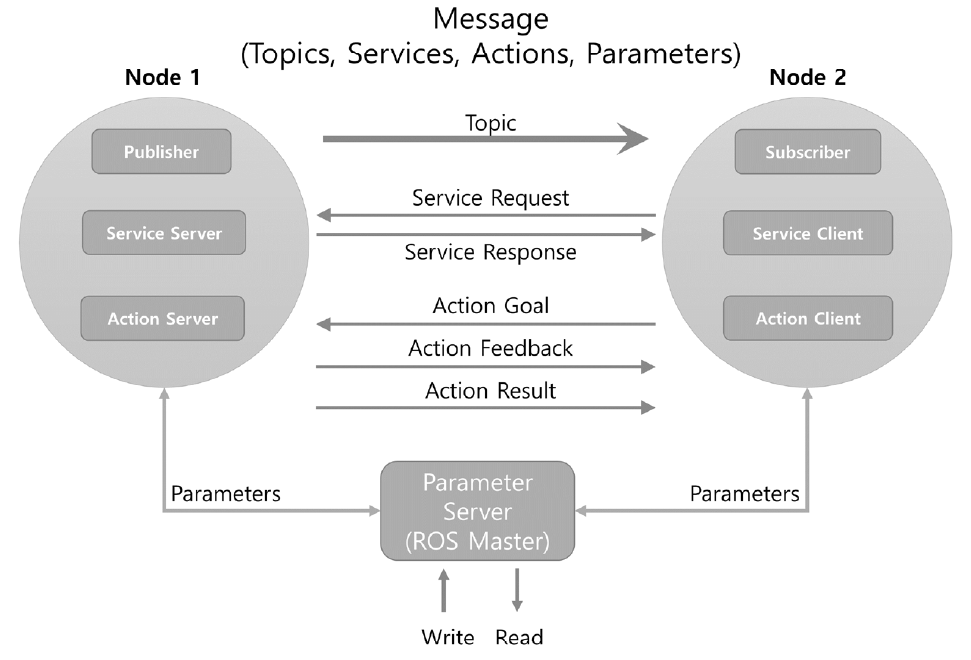
\includegraphics[width=1.0\linewidth]{Main/Chapter3/Images3/n_s_a_14.PNG}
                \caption{Comunicación de mensajes entre nodos \cite{ROS_BOOK_1}}
                \label{f:Cap3_conceptos_14}
            \end{figure}   

               \newpage
               
            \subsubsection{Nivel Comunitario}
            
            El ecosistema ROS ahora consta de decenas de miles de usuarios en todo el mundo, que trabajan en dominios que van desde proyectos de pasatiempos de mesa hasta grandes sistemas de automatización industrial. 
            Una característica importante de ROS es la comunidad que comparte software y código, lo que convierte a ROS en una de las comunidades de robots más grandes. Hay diferentes formas de obtener recursos ROS:

            \begin{figure}[htb]
                \centering
                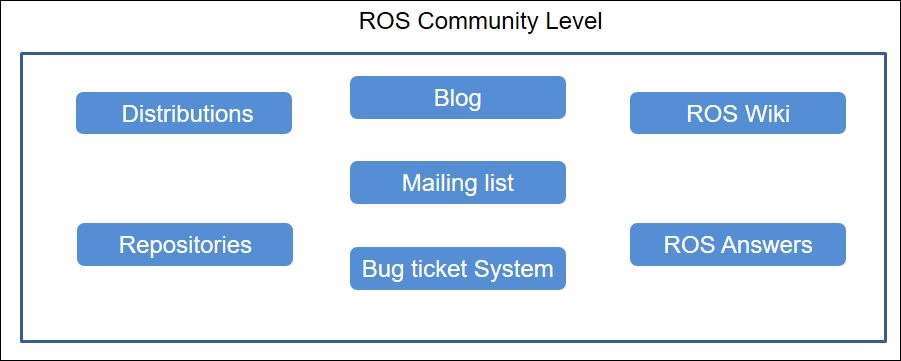
\includegraphics[width=0.9\linewidth]{Main/Chapter3/Images3/n_s_a_15.png}
                \caption{Nivel comunitario de ROS \cite{lentin_2017}}
                \label{f:Cap3_conceptos_15}
            \end{figure}        
            
            \begin{itemize}
                \item {\textbf{Distribuciones:} las distribuciones ROS son colecciones de stacks versionadas que puede instalar. Las distribuciones juegan un papel similar a las distribuciones de Linux: facilitan la instalación de una colección de software y también mantienen versiones consistentes en un conjunto de software. (http://wiki.ros.org/Distributions)}
                \item {\textbf{Repositorios:} ROS se basa en una red federada de repositorios de código, donde diferentes instituciones pueden desarrollar y lanzar sus propios componentes de software de robot. }
                \item {\textbf{El ROS Wiki:} La Wiki de la comunidad de ROS es el foro principal para documentar información sobre ROS. Cualquiera puede registrarse para obtener una cuenta y contribuir con su propia documentación, proporcionar correcciones o actualizaciones, escribir tutoriales y más. (http://wiki.ros.org/) }
                \item {\textbf{Mailing Lists:} Listas de correo de usuarios ROS}
                \item {\textbf{Answers:} Página web donde los usuarios comparten preguntas, respuestas y comentarios. (https://answers.ros.org/) }
                \item {\textbf{Blog ROS:} Noticias de la comunidad ROS. (www.ros.org/news/)  }
                \item {\textbf{ROS Discourse:} es el foro de discusión de la comunidad (https://discourse.ros.org/). No es para cuestiones técnicas específicas, sino para temas, anuncios y noticias más amplio.}
            \end{itemize}
            
            
            
            
               \newpage
               
    \newpage

    \subsection{Herramientas}
    
        Existen varias herramientas que pueden ayudarnos a la hora de usar ROS. Debemos tener en cuenta estas herramientas GUI como complementarias a las herramientas de línea de comandos. Hay una gran cantidad de herramientas ROS, incluidas las herramientas que los usuarios de ROS también han lanzado personalmente. Entre estas herramientas, las que discutiremos en este capítulo no procesan directamente una función en el ROS, pero son herramientas complementarias muy útiles para programar con ROS.
            
        \subsubsection{Launch Files}
            En un proyecto ROS, es posible que desee ejecutar varios nodos ROS al mismo tiempo para realizar sistemas más complejos. ROS tiene una herramienta llamada roslaunch que permite a los usuarios ejecutar numerosos nodos, establecer parámetros de configuración de cada nodo, renombrar los nombres de temas predeterminados e incluso cambiar el nombre del nodo. El propósito de esto es configurar fácilmente el sistema global.
            
        \subsubsection{RQT Graph}
            Proporciona visualización de un sistema ROS, mostrando los nodos y las conexiones entre ellos que permite depurar y comprender el sistema en ejecución y cómo está estructurado. 
            
            \begin{figure}[htb]
                \centering
                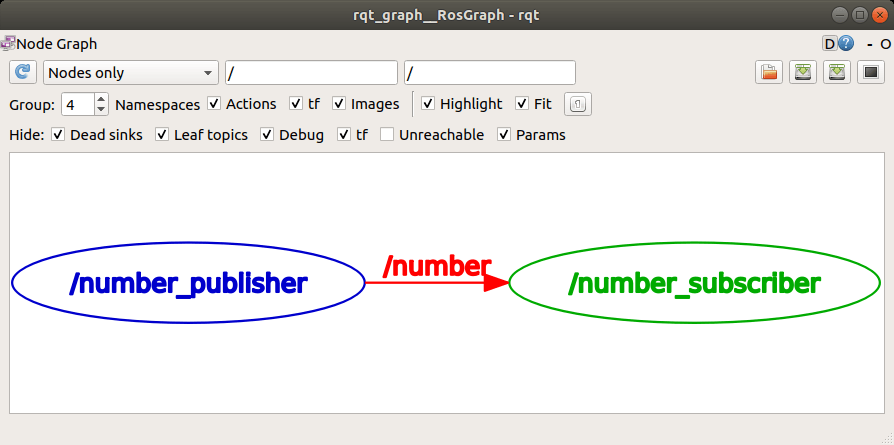
\includegraphics[width=1.0\linewidth]{Main/Chapter3/Images3/herramientas_1.png}
                \caption{Visualización de la comunicación entre un nodo publisher y el nodo subscriber a travez del tema number en RQT Graph.}
                \label{f:Cap3_herramientas_1}
            \end{figure}       
            
            
    \newpage    
    
            \subsubsection{RQT Rosbag}
                Rosbag es un conjunto de herramientas para grabar y reproducir datos de temas ROS. Los datos se almacenan en archivos de bag y hay disponibles herramientas de línea de comandos para trabajar con bag. Rosbag evita la deserialización y reserialización de mensajes y sus principales herramientas son:
                
                    \begin{itemize}
                        \item{\textbf{rosbag info:} Muestra el contenido de los archivos de la bolsa, como temas grabados, hora de inicio y finalización, número de mensajes, frecuencia y estadísticas de compresión} 
                        \item{\textbf{rosbag record:} Escribe el contenido de todos los mensajes publicados sobre esos temas que queremos registrar y la información se almacena en un archivo .bag.} 
                        \item{\textbf{rosbag play: } Lee un archivo de bolsa y publica la información sobre temas ROS de forma sincronizada en el tiempo. El sistema ROS puede utilizar esta información como si fuera en tiempo real.} 
                    \end{itemize}

            \subsubsection{RQT reconfigure}
Adaptación del paquete “Dynamic reconfigure” que permite modificar en tiempo real todos los parámetros de los nodos, para realizar modificaciones rapidas. La configuración de los parámetros se puede exportar para utilizar en el futuro.

            \subsubsection{MoveIt }
 Software basado en la planificación del movimiento, que considera prospección 3D, cinemática, control y navegación. Proporciona una plataforma para el desarrollo de aplicaciones robóticas, evalúa nuevos diseños de robots y productos para la construcción robótica integrado para aplicaciones industriales, I + D, etc.
 
             \begin{figure}[htb]
                \centering
                
\includegraphics[width=0.8\linewidth]{Main/Chapter3/Images3/herramientas_2.png}
                \caption{Logo Proyecto MoveIt}
                \label{f:Cap3_herramientas_2}
            \end{figure}     
            
        \newpage    

            \subsubsection{Gazebo}
     Es un simulador virtual que brinda la posibilidad de realizar simulaciones de algoritmos, diseños de robots y ejecutar pruebas dentro de escenarios reales con precisión y eficiencia. Proporciona un motor de física robusto, gráficos de alta calidad e interfaces gráficas. 
        
        \begin{figure}[htb]
                \centering
                
\includegraphics[width=0.3\linewidth]{Main/Chapter3/Images3/herramientas_4.png}
                \caption{Logo Gazebo}
                \label{f:Cap3_herramientas_4}
        \end{figure} 
    
        
        \begin{figure}[htb]
                \centering
                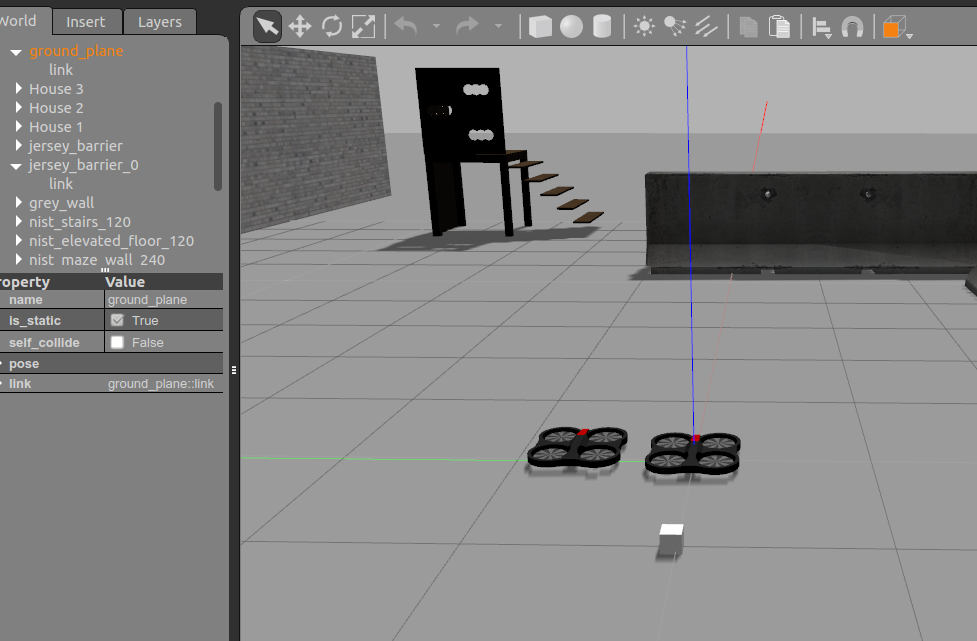
\includegraphics[width=0.98\linewidth]{Main/Chapter3/Images3/herramientas_3.png}
                \caption{Simulación de dron en Gazebo}
                \label{f:Cap3_herramientas_3}
        \end{figure}  

    
        \newpage    



\section{Visualización}
    
    \subsection{Interfaz de visualización gráfica ROS visualization (Rviz)}

        RVIZ es la abreviación de ROS visualización. Es un entorno de visualización 3D de uso general para robots, sensores y algoritmos. Permite visualizar mapas, robots, objetos, datos láser, imágenes de cámaras, nubes de puntos y marcadores.   Como la mayoría de las herramientas ROS, se puede utilizar para cualquier robot y configurar rápidamente para una aplicación en particular.
        
        \begin{figure}[htb]
            \centering
            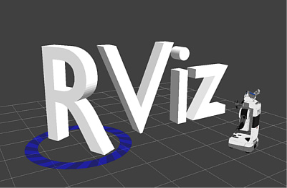
\includegraphics[width=0.35\linewidth]{Main/Chapter3/Images3/3-6/logo-rviz.png}
            \caption{Logo de Rviz}
            \label{f:Cap3-6_logo_rviz}
        \end{figure}
        
        RVIZ proporciona una interfaz sencilla para elegir la información que queremos que se muestre. La Figura 3.2 muestra un ejemplo de la interfaz RVIZ. A la izquierda podemos ver todos los elementos que muestra RVIZ. Cada elemento debe configurarse con el nombre de un tema específico. Entonces RVIZ se suscribe a ese tema y visualiza su información. En el medio está la ventana principal donde se muestra toda la información y a la izquierda podemos elegir las propiedades de la herramienta y cambiar entre diferentes vistas. RVIZ también permite al usuario crear complementos para agregar nuevas capacidades de visualización.
        
        \begin{figure}[htb]
            \centering
            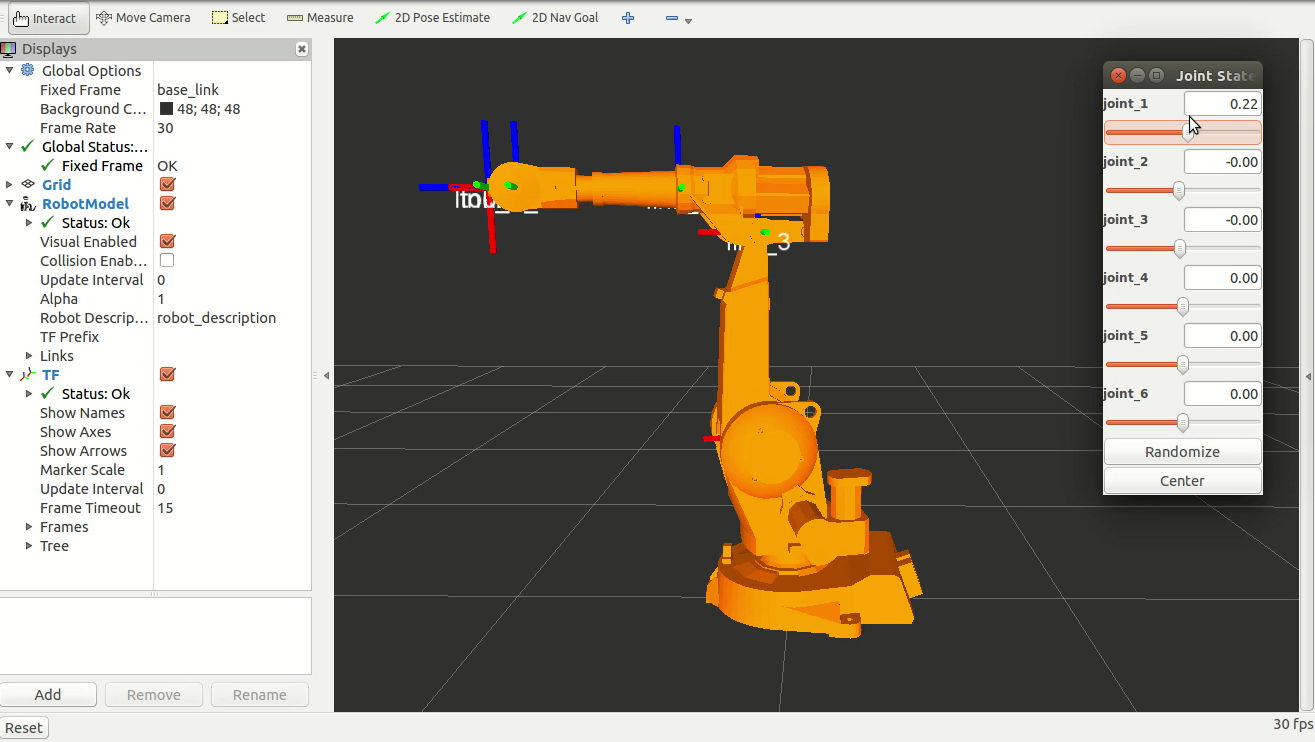
\includegraphics[width=0.8\linewidth]{Main/Chapter3/Images3/interfaz-rviz.png}
            \caption{ABB IRB 2400 con publicador de estado de juntas en RViz \cite{lentin_20188}}
            \label{f:Cap3-6_interfaz_rviz}
        \end{figure}
        
        \newpage
    
    \subsection{Coordenadas TF}
    
        Un marco de coordenadas o frame es un concepto importante en ROS. Cualquier robot puede tener varios componentes, como un láser, una cámara, un sonar o brazos, y pueden tener un marco de coordenadas adjunto. Muchos algoritmos ROS requieren realizar un seguimiento de todos estos marcos de coordenadas.
        
        TF son las siglas en ingles de marco de transformadas (Transform frames) y es una de las librerías fundamentales de ROS. TF está diseñada para proporcionar una forma estándar de realizar un seguimiento de los marcos de coordenadas y transformar los datos dentro de todo el sistema a lo largo del tiempo. El paquete TF puede rastrear y mantener la relación entre múltiples marcos de coordenadas. Su función es proporcionar herramientas y funciones para definir todos los marcos de coordenadas de nuestro robot y transformar datos de un marco a otro, como por ejemplo puntos o vectores.
        
        \begin{figure}[htb]
            \centering
            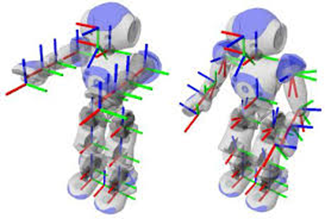
\includegraphics[width=1.0\linewidth]{Main/Chapter3/Images3/3-6/ejemplo-multiples-frames-rviz.png}
            \caption{Tres visualizaciones diferentes del modelo Minibot URDF. Visualizacion en Rviz, modelo de coliciones y estructura tf  \cite{phdthesistfhuman}. }
            \label{f:Cap3-6_frames_rviz}
        \end{figure}
        
Un ejemplo para explicar las coordenadas tf es el del robot simple  mostrado en la figura \eqref{f:Cap3-6_nose1}, que tiene una base móvil con un láser montado encima. El objetivo de este robot es evitar obstáculos para no colisionar, como una pared.
En referencia al robot, se definen dos marcos de coordenadas: uno correspondiente al punto central de la base del robot llamado ''base\_link''y otro para el punto central del láser que está montado en la parte superior de la base movil llamado ''base\_laser''. 

El láser recopila datos en forma de distancias desde el punto central del láser a una pared, es decir, el láser tiene datos de distancia en el marco de coordenadas ''base\_laser''. Para evitar obstáculos se debe mover la base móvil, por los que los datos del láser se deben transformar al sistema de referencia ''base\_link'', en otras palabras,  se tiene que definir una relación entre los marcos de coordenadas ''base\_laser'' y ''base\_link''.
 \newpage
 
        \begin{figure}[htb]
            \centering
            \includegraphics[width=1.0\linewidth]{Main/Chapter3/Images3/simple_robot.png}
            \caption{Ejemplo robot simple compuesto por base móvil y un láser}
            \label{f:Cap3-6_nose1}
        \end{figure}    

Esta relación entre los marcos de referencia son desplazamiento de traslación y rotacional entre los marcos 'base\_laser'' y ''base\_link''. Gestionar esta relación en todo momento en una simulación del robot , es decir, almacenar y aplicar los desplazamientos adecuados entre los fotogramas en cada momento, se convierte en un verdadero problema a medida que aumenta el número de fotogramas de coordenadas. Afortunadamente, sin embargo, no se tiene que hacer este trabajo ya que en su lugar, se define la relación entre "base\_link" y "base\_laser" una sola vez usando tf y la bibloteca tf gestiona la transformación entre los dos marcos de coordenadas automáticamente.

Para definir y almacenar la relación entre los marcos ''base\_link'' y ''base\_laser'' usando tf, se necesita crear a un árbol de transformación. Conceptualmente, cada nodo en el árbol de transformación corresponde a un marco de coordenadas y cada borde corresponde a la transformación que debe aplicarse para pasar del nodo actual a su hijo. Tf usa una estructura de árbol para garantizar que haya un solo recorrido que vincule dos marcos de coordenadas cualesquiera, y asume que todos los bordes del árbol se dirigen desde los nodos principales a los secundarios.    


        \begin{figure}[htb]
            \centering
            \includegraphics[width=1.0\linewidth]{Main/Chapter3/Images3/tf_robot.png}
            \caption{Láser recolectando datos respecto a ''base\_laser'', árbol de transformación y datos del láser transformados a marco ''base\_link'' }
            \label{f:Cap3-6_nose1}
        \end{figure}    
        
        
         TF ofrece una serie de herramientas o aplicaciones que facilitan al usuario la visualización del estado de las transformadas como:
        
        \begin{itemize}
            \item \textbf{tf\_monitor:} Imprime la información sobre el árbol de transformación actual.
            \item \textbf{tf\_echo:} Imprime información sobre la transformación entre dos fotogramas.
            \item \textbf{tf\_tree:} Crea un gráfico visual del árbol de transformación (en formato pdf).
        \end{itemize}
        
        \newpage
        La figura \eqref{f:Cap3-6_sistema_arbol_tf} muestra un ejemplo de un árbol de transformada haciendo uso de la herramienta rqt\_tf\_tree y la figura \eqref{f:Cap3-6_NOSE_tf} los respectivos marcos de referencia de cada parte del robot . En las dos figuras se puede observar los distintos frames del sistema y sus relaciones.
        
        \begin{figure}[htb]
            \centering
            \includegraphics[width=0.7\linewidth]{Main/Chapter3/Images3/3-6/ejemplo-frames-sistema-arbol.png}
            \caption{Frames de un sistema visualizado mediante tf\_tree}
            \label{f:Cap3-6_sistema_arbol_tf}
        \end{figure} 
        
        
        \begin{figure}[htb]
            \centering
            \includegraphics[width=0.55\linewidth]{Main/Chapter3/Images3/3-6/nose2.png}
            \caption{Figura que contiene los marcos tf más utilizados \cite{10.5555/2904061}}
            \label{f:Cap3-6_NOSE_tf}
        \end{figure} 
        
    
        Resumiendo esta sección, TF es una biblioteca con las siguientes características:
        
        \begin{itemize}
            \item Es una herramienta para realizar un seguimiento de los marcos de coordenadas a lo largo del tiempo.
            \item Mantiene la relación entre los marcos de coordenadas en una estructura de árbol almacenada en el tiempo
            \item Permite al usuario transformar puntos y vectores entre marcos de coordenadas en cualquier momento deseado
            \item Es implementado como modelo de publisher/subscriber en los temas con nombres /tf y /tf\_statics
        \end{itemize}
        
                        \newpage

    \subsection{Unified Robot Description Format (URDF)}\label{cap2_urfdf}
    
        \subsubsection{Introducción URDF}
    
        En ROS, es posible visualizar un modelo de un robot mediante el uso de archivos de formato de descripción de robot unificado (URDF). Sin embargo, solo aquellos robots que tienen eslabones rígidos conectados mediante articulaciones pueden ser descritos mediante modelos URDF.  Se puede usar un modelo URDF para calcular la cinemática, agregar nuevos marcos de coordenadas y moverlos de acuerdo con los valores del codificador del robot. Además, puede incluir otras propiedades físicas como inercia, colisiones, dinámica de articulaciones, etc. 
        
        Los archivos URDF están basados en XML y como tal, están compuestos por etiquetas de XML especiales que pueden ser leídas para extracción de información. A la lectura del archivo para extraer la información importante del modelo se denomina parsing y al programa o función que lo realiza, parser.
        
        La descripción del modelo consiste básicamente en de unir dos conjuntos: el conjunto de enlaces (link) y el conjunto de uniones (Joint). La forma de construir y visualizar un modelo de robot en URDF es escribir y compilar el archivo URDF. Una vez que se crea la representación 3D de un robot mediante el uso de un archivo URDF, es posible utilizar dicha representación para simular el movimiento del robot. Para ello, el usuario debe publicar las condiciones del robot en TF, utilizando un nodo (o nodos) para publicar la información de transformación.
        
        \begin{figure}[htb]
            \centering
            \includegraphics[width=0.55\linewidth]{Main/Chapter3/Images3/3-7/representacion-de-eslabon-en-urdf.png}
            \caption{Elementos basicos de visualization URDF: links y joints \cite{urdftutorials}.}
            \label{f:Cap3-7_eslabon_urdf}
        \end{figure} 
        
                                \newpage

        
        \subsubsection{Links}
        
        Los eslabones o enlaces (conjunto link) describen la parte física rígida del robot y permite especificar sus propiedades, como tamaño, forma, color o una malla 3D compleja importada. Consta de tres elementos:
    
        \begin{figure}[htb]
            \centering
            \includegraphics[width=0.8\linewidth]{Main/Chapter3/Images3/3-7/eslabon2.png}
            \caption{Reparcelación de la visual, inercia y colisión de un link con sus respectivos marcos de referencia para urdf  \cite{urdftutorials}}
            \label{f:Cap3-7_noseee_urdf}
        \end{figure} 

        \begin{enumerate}
            \item \textbf{Inertial:} Especifica las propiedades inerciales del link (posición del centro de masas, la masa y la matriz Inercia)
            \item \textbf{Visual:} en este elemento viene especificado como debe estar representado el link. Es posible usar solidos simples como una esfera o un cilindro, o hacer representaciones más trabajadas como mallados o nube de puntos. Del mismo modo, también y se pueden definir los colores e importar texturas.
            \item \textbf{Collision:} Describe las propiedades de colisión de los links. Puede ser una forma diferente a la visual, como una figura más simple que sea representativa, a fin de reducir los tiempos de calculo en las simulaciones.
        \end{enumerate}
        
        \begin{figure}[htb]
            \centering
            \includegraphics[width=0.9\linewidth]{Main/Chapter3/Images3/3-7/codigo.png}
            \caption{Descripción de un link en código URDF}
            \label{f:Cap3-7_nose_nose}
        \end{figure} 
        
                                \newpage

        
        \subsubsection{Joints}
        
        Las articulaciones o uniones (conjunto joint) indican la relación entre los distintos eslabones del robot. Describen además la cinemática y dinámica de cada articulación, además de especificar los límites de colisión del robot. Una articulación queda fefinida cuando se especifican los eslabones que une: el primero es llamado el padre (parent) y el segundo el hijo (child).
        
        \begin{figure}[htb]
            \centering
            \includegraphics[width=0.65\linewidth]{Main/Chapter3/Images3/3-8/representacion-de-una-articulacion-en-URDF.png}
            \caption{Representación gráfica de un joint y su relación padre-hijo con los link \cite{urdftutorials}}
            \label{f:Cap3-8_nose_nose}
        \end{figure} 
        
        Tipos de articulaciones:
        
        \begin{enumerate}
           \item \textbf{Revolute:} Permite que dos sólidos giren alrededor de un eje común y tiene un giro limitado especificado por un límite superior y uno inferior.
            \item \textbf{Continuous:} Se trata de una articulación de Revolute pero sin límites..
            \item \textbf{Prismatic:} Una junta que se deslizarse a lo largo de un eje. Tiene un alcance acotado por un límite inferior y uno superior.
            \item \textbf{Fixed:} No es realmente una articulación porque impide el movimiento. La unión no tiene ningún grado de libertad. Este tipo de articulación no requiere de ninguno de los elementos que describe la articulación..
            \item \textbf{Floating:} Esta unión mantiene libres todos los grados de libertad..
            \item \textbf{Planar:} Articulación que permite el movimiento en un plano.
        \end{enumerate}
        
                                        \newpage

        
        \begin{figure}[htb]
            \centering
            \includegraphics[width=1.0\linewidth]{Main/Chapter3/Images3/3-8/codigo-joint.png}
            \caption{Descripción de un joint en código URDF}
            \label{f:Cap3-8_nose_nose}
        \end{figure} 
        
        Cada conjunto de uniones (joint) está compuesto por hasta nueve elementos:
        
         \begin{enumerate}      
            \item \textbf{Origin:} es la posición donde se encuentra la unión entre el sólido padre (Parent) y el sólido hijo (child), en referencia al primero.
            \item \textbf{Parent:} el objeto padre en una unión
            \item \textbf{Child:} en objeto hijo en una unión
            \item \textbf{Axis:} eje del articulacion en la referencia global.
            \item \textbf{Calibration:} es un elemento opcional. Sirve para determinar la posición absoluta de la articulación
            \item \textbf{Dynamics:} es un elemento opcional. Define la amortiguación y la fricción de la articulación.
            \item \textbf{Límite:} sólo obligatoria en las articulaciones de revolución y en las prismáticas. Define el límite inferior y superior de la articulación, el esfuerzo máximo que puede aplicar y la velocidad máxima de esta.
            \item \textbf{Mimic:} es un elemento opcional. Se usa para especificar que una articulación imita a otra articulación ya existente. 
            \item \textbf{Safety controller:} es un elemento opcional. Específica para qué valores debe empezar a limitar la posición o la velocidad de una articulación en función de los límites establecidos en el tag <límit>.
        \end{enumerate}
        
                                                \newpage

    \subsection{Herramientas complementarias}
    
        Algunos paquetes y herramientas utiles para la interaccion con modelos URDF son los siguientes:
      
        \begin{itemize}
            \item \textbf{Joint\_state\_Publisher:} Este paquete contiene un nodo del mismo nombre que lee la descripción del modelo del robot, encuentra todas las articulaciones (joints) y publica los valore articulares para todas las articulaciones movibles usando sliders.
            \item \textbf{robot\_state\_Publisher:} Este paquete lee el estado de las articulaciones del robot y publica las posiciones y orientaciones 3D de cada eslabón usando la cinemática obtenida a partir del URDF. La posición 3D del robot se publica como una transformación (tf) que define las relaciones entre los sistemas de coordenadas.
            \item \textbf{xacro:} Significa Xml mACROs y es un formato que permite utilizar variables y otros add-ons para la generación de modelos complejos en formato URDF. De esta forma los modelos pueden ser más fáciles de entender y más mantenibles.
        \end{itemize}      
        
        La herramienta urdf\_to\_graphiz sirve para para obtener un diagrama graphviz de su archivo urdf, tal como se aprecia en la figura \eqref{f:Cap3-9_nose_nose}:
        
        \begin{figure}[htb]
            \centering
            \includegraphics[width=0.43\linewidth]{Main/Chapter3/Images3/3-9/Esquema-de-los-componentes-de-un-fichero-urdf.png}
            \caption{Ejemplo de la representación gráfica URDF de un robot por medio de la herramienta urdf\_to\_graphiz \cite{urdftutorials}}
            \label{f:Cap3-9_nose_nose}
        \end{figure} 
        
    \newpage

\section{ADAMS (Automated Dynamic Analysis of Mechanical Systems)}

    % Adams es el software de análisis de movimiento y dinámica multicuerpo más utilizado en el mundo. Adams ayuda a los ingenieros a estudiar la dinámica de las piezas móviles, cómo se distribuyen las cargas y fuerzas en los sistemas mecánicos y a mejorar y optimizar el rendimiento de sus productos. El software de dinámica multicuerpo de Adams permite a los ingenieros crear y probar fácilmente prototipos virtuales de sistemas mecánicos en una fracción del tiempo y el costo necesarios para la construcción y prueba físicas. A diferencia de la mayoría de las herramientas integradas de CAD, Adams incorpora la física real resolviendo simultáneamente ecuaciones de cinemática, estática, cuasi-estática y dinámica. Al utilizar la tecnología de solución de dinámica multicuerpo, Adams también ejecuta dinámica no lineal en una pequeña fracción del tiempo requerido por las soluciones FEA. Las cargas y fuerzas calculadas por las simulaciones de Adams mejoran la precisión de FEA al proporcionar una mejor evaluación de cómo varían en una amplia gama de entornos operativos y de movimiento.
    
    \subsection{Historia}
    ADAMS significa Análisis dinámico automático de sistemas mecánicos y fue desarrollado originalmente por Mechanical Dynamics
    Inc. (MDI). MDI fue formado por investigadores / desarrolladores del código ADAMS original en la Universidad de Michigan, Ann
    Arbor, MI, Estados Unidos. Más tarde, fue absorbida por McNeil Schindler Corp (MSC) en 2002.
    
    En el núcleo de ADAMS hay un código de gran desplazamiento llamado ADAMS / Solver, que resuelve ecuaciones numéricas no lineales.
    En ese entonce los modelos se creaban en formato de texto y luego se enviaban a ADAMS / Solver. 
    
    A principios de los 90, se lanzó ADAMS / View, que permitió a los usuarios crear, simular y examinar resultados en un único entorno gráfico de usuario (GUI). Hoy, MSC produce
    muchos paquetes de análisis de ingeniería general como MSC.NASTRAN, MSC.PATRAN, MSC.DYTRAN, etc. y también paquetes
    que atienden a usuarios específicos de la industria como MSC.ADAMS / Car, MSC.ADAMS / Rail, MSC.ADAMS / Engine, etc.
    
     \subsection{introducción}

    Adams es un programa para simulación dinámica y análisis de movimiento cinemático en múltiples cuerpos. Ayuda en el estudio de la dinámica de las partes móviles, como cargas y fuerzas que se distribuyen a lo largo de los sistemas mecánicos, para mejorar y optimizar el rendimiento de los productos. Permite  crear y probar prototipos virtuales de los sistemas mecánicos en una fracción del tiempo y costo requerido para la estructura física y la prueba, incorporando la física real de forma simultánea a la resolución de ecuaciones de cinemática, estática, y la dinámica.

    % Adams ejecuta la dinámica no lineal en una fracción del tiempo requerido por las soluciones de FEA. Proporcionando una mejor evaluación de la forma en que varían a través de una gama completa de movimiento y entornos operativos.
    
    % Los módulos opcionales e integrados con Adams permiten a los usuarios integrar los componentes mecánicos, neumática, hidráulica, electrónica y tecnologías de control de sistemas para construir y probar prototipos virtuales que representan con precisión las interacciones entre estos subsistemas.
    



    % \subsection{Análisis de sistemas multicuerpo}
    
    Un \textbf{sistema multicuerpo} es la modelización de un sistema mecánico como un conjunto de sólidos rígidos o flexibles conectados entre sí por un conjunto de uniones. Este conjunto forma un sistema físico cuya cinemática y dinámica se pueden describir con una serie de ecuaciones diferenciales y algebraicas.\cite{cap3:adams-dinamica_multicuerpo}
    
    Excepto en el caso de sistemas mecánicos muy sencillos, la resolución de las ecuaciones que describen el movimiento de un sistema multicuerpo requiere con frecuencia la ayuda de programas informáticos de cálculo numérico. Por este motivo, la simulación y el análisis de sistemas multicuerpo están estrechamente ligados a disciplinas como el álgebra lineal y la programación.
    
    Hoy en día existen diversos programas que se encargan de darle un aspecto mas visual a todas las ecuaciones subyacentes por debajo en la resolución de este tipo de sistemas, en nuestra tesis utilizaremos ADAMS, dado que se puede adquirir bajo una licencia estudiantil por un semestre, previa creación y validación de una \href{https://www.mscsoftware.com/page/adams-student-edition}{cuenta universitaria}.
    
    Pese a que nuestra hipótesis nos guía a regirnos solo por software libre, esto preocupa sobretodo en la formulación, en la validación hemos intentado ocupar los mejores estándares para verificar los códigos propuestos.
    
    
    \begin{figure}[htb]
        \centering
        \includegraphics[width=1\linewidth]{Main/Chapter3/Images3/adams/logo_adams.png}
        \caption{Iamgen de referencia del software Adams}
        \label{f:Cap3-adams_logo}
    \end{figure} 
    
    
    \subsection{Descripción del ambiente de ADAMS}
    
    La versión actualizada de ADAMS trabajada durante la tesis es la 2020 FP1, y la descripción del ambiente se hará bajo el sistema operativo Windows dada su extensión, y con el fin de llegar a la mayor cantidad de personas.
    
        \subsubsection{Inicio de un nuevo modelo y su configuración}
        
            Al iniciar ADAMS lo primero que encontraremos sera el dialogo de bienvenida mostrado en la figura \ref{f:Cap3-adams_window_bienvenida}, la ventana nos da tres opciones, New Model, para iniciar un nuevo modelo; Existing Model para abrir la base de datos de un modelo existente (los archivos ADAMS tienen extensión .bin) y finalmente la opción exit, para cerrar ADAMS. 
            
            \begin{figure}[H]
                \centering
                \includegraphics[width=0.7\linewidth]{Main/Chapter3/Images3/adams/Dialogo_Bienvenida.png}
                \caption{Ventana de bienvenida al iniciar ADAMS}
                \label{f:Cap3-adams_window_bienvenida}
            \end{figure} 
            
            En el fondo de la ventana de bienvenida, ya podemos observar con antelación el GUI de ADAMS, pero no podremos interactuar con el, hasta terminar la configuración inicial del modelo.
            Para iniciar un nuevo modelo, damos clic en \textbf{New Model}, y se deplegará la ventana de configuración inicial que se muestra en la figura \ref{f:Cap3-adams_window_configuracion_inicial}. Las configuraciones posibles son:
            
                \begin{itemize}
                    \item \textbf{Moedel name:} El nombre del modelo
                    \item \textbf{Gravity:} Aquí se configura la fuerza de gravedad, tenemos tres posibiloidades:
                           \begin{itemize}
                               \item Earth Normal (-Global Y): Gravedad normal de 1G (9,81 $\frac{m}{s^2}$) en dirección -Y. Es posible cambiar este valor en cualquier momento dentro del modelo.
                               \item No gravity: El modelo no contara con fuerza de gravedad.
                               \item Other: Permite que uno ajuste la gravedad como se desee. El cuadro de diálogo Configuración de gravedad aparece después de terminar la configuración inicial.
                           \end{itemize}
                    \item \textbf{Units:} El sistema de medición empleado en el modelo, ADAMS permite varias posibilidades:
                        \begin{itemize}
                            \item MMKS: Largo en milímetros, masa en kilogramos y fuerza en Newton.
                            \item MKS: Largo en metros, masa en kilogramos y fuerza en Newton.
                            \item CGS: Largo en centímetros, masa en gramos y fuerza en Dyne.
                            \item IPS: Largo en pulgadas, masa en slug y fuerza en libras
                        \end{itemize}
                    \item \textbf{Working Directory:} El directorio donde se guardaran todos los datos y archivos del modelo.
                \end{itemize}
            
            \begin{figure}[H]
                \centering
                \includegraphics[width=0.7\linewidth]{Main/Chapter3/Images3/adams/ventana_configuracion_inicial.png}
                \caption{Ventana de bienvenida al iniciar ADAMS}
                \label{f:Cap3-adams_window_configuracion_inicial}
            \end{figure} 
            
            Luego de darle una configuración inicial a nuestro modelo, inicia la ventana principal de ADAMS, la cual se observa en la figura \ref{f:Cap3-adams_window_GUI}. A continuación se detallan sus principales puntos de interés: (NO ME GUSTA COMO QUEDO, PERO CORREGIRÉ DESPUÉS, DEBERÍAN IR LOS NOMBRES EN VEZ DE LOS NÚMEROS)
            
            \begin{enumerate}
                \item Menu principal
                \item Barra de herramientas principal
                \item Árbol del modelo
                \item Barra de herramientas de estado
            \end{enumerate}
            
            \begin{figure}[H]
                \centering
                \includegraphics[width=1\linewidth]{Main/Chapter3/Images3/adams/interfaz_vista_adams.png}
                \caption{Interfaz de vista en ADAMS}
                \label{f:Cap3-adams_window_GUI}
            \end{figure} 
            
            
            
            
            
    \subsection{Modelo y estructura de los datos en ADAMS}
        
        
        \subsubsection{Convención de nombres en ADAMS}
        
        \subsubsection{Sistemas de coordenadas}
        
        \subsubsection{Parts}
        % \paragraph{Geometria}
        
        \begin{itemize}
            \item \textbf{Geometry:} asd
            \item \textbf{Markers:} asd
            \item \textbf{Construction Points:} asd
        \end{itemize}

        
        \subsubsection{Constrains}
        
        \subsubsection{Measures}
        
        \subsubsection{Forces}
        
    
    \subsection{Simulación}
    
        \subsubsection{Analyses}
        
        \subsubsection{Results Sets}
        
        \subsubsection{Components}
    
            
    
    
    


% COPY PASTE DE VARIOS PAPEOS, PARA POSTERIOR MEJORA Y INTRODUCCIÓN AL CONTEXTO DE NUESTRA TESIS

    % La simulación de sistemas robotizados esta íntimamente ligada a la potencia
    % computacional de los procesadores de cálculo. El gran avance producido
    % con los microprocesadores actuales, ha permitido el desarrollo de diferentes
    % paquetes de simulación dinámica capaces de simular el comportamiento dinámico
    % de casi cualquier mecanismo multicuerpo. En esta tesis, el modelo del robot delta en estudio es construido en ADAMS.
    
    


    

    
    

    

    
      
        
            
            
            

        
    
        % Teoria herramientas
}
{\hypersetup{colorlinks=true,        
    linkcolor=blue,         
    filecolor=magenta,       
    urlcolor=russet,           
    citecolor=blue}
%\chapter{Modelación física y matemática}\label{CAP4}
    
\section{Desarrollo de modelación y metodologías}
    En primero lugar, con el objetivo de modelar la cinemática y la dinámica de un robot delta de manera veraz, se presentan 2 metodologías que son programadas y comparadas en este texto. Estas dos metodologías deben dar los mismos resultados. Se les llama metodología A y metodología B. Las etapas de las 2 metodologías tienen el mismo objetivo, sin embargo, el planteamiento del problema cinemático y dinámico es tratado de forma diferente. Para comparar las dos metodologías se crea un marco de referencia global en el robot delta. Por ende, en los códigos de los algoritmos es necesario que las salidas o resultados estén en correlación a este sistema de referencia. En la siguiente imagen, se muestra un diagrama de flujo de las 2 metodologías, con el objetivo de cada etapa y el titulo-autor de donde se recopila información.
    
        
        \begin{figure}[htb]
             \centering
             \includegraphics[width=0.5\linewidth]{Main/Chapter4/Images4/Metodologia.png}
              \caption{Fotografía de un paraguas}
              \label{f:Cap4_metodologia}
        \end{figure}
    
         \newpage


    En segundo lugar, se explica que es un espacio de trabajo para un robot delta y los parámetros que influyen en su volumen, forma, densidad espacial, etc. Para ello, se utiliza la modelación cinemateca y se privilegia la metodología A sobre la B por razones con relación a el cálculo del jacobiano que se explican en dicha sección.
    
        \begin{figure}[htb]
             \centering
             \includegraphics[width=0.7\linewidth]{Main/Chapter4/Images4/Metodologia_ws.png}
              \caption{Fotografía de un paraguas}
              \label{f:Cap4_metodologia_ws}
        \end{figure}
    
    Por último, se presentan las trayectorias más comunes implementadas en el desarrollo de los robots. De todas las trayectorias presentadas se profundizan 2, las que en esta tesis se utilizan para simular el mecanismo del robot delta y comparar los resultados de la modelación cinemateca y dinámica.
    
        \begin{figure}[htb]
             \centering
             \includegraphics[width=0.7\linewidth]{Main/Chapter4/Images4/Metodologia_tray.png}
              \caption{Fotografía de un paraguas}
              \label{f:Cap4_metodologia_tray}
        \end{figure}  
    
     \newpage


\section{Nomenclatura y sistemas de referencia global}

        \begin{figure}[htb]
             \centering
             \includegraphics[width=0.7\linewidth]{Main/Chapter4/Images4/ref1.jpg}
              \caption{Fotografía de un paraguas}
              \label{f:ref1}
        \end{figure}

     \newpage

\section{Metodología A}

    \subsection{Modelacion Cinemática de Posición}
    
        En esta sección, se da a conocer una solución para calcular la cinemática inversa y cinemática directa de un robot paralelo tipo delta. Con el fin de solucionar el problema cinemático, se emplean las ideas y modelación del robot delta propuestas por la referencia bibliográfica \cite{Diseno_e_implementacion_de_un_sistema_de_control_para_la_representacion_grafica_a_partir_de_imagenes}.
        
        \subsubsection{Nomenclatura de Parámetros Geométricos y Sistema de Referencia Local}

        \begin{figure}[htb]
             \centering
             \includegraphics[width=0.5\linewidth]{Main/Chapter4/Images4/Metodo_A_Modelacion_Cinematica_Posicion_1.png}
              \caption{Fotografía de un paraguas}
              \label{f:Cap4_Metodo_A_Modelacion_Cinematica_Posicion_1}
        \end{figure}

 

        En la figura \ref{f:Cap4_Metodo_A_Modelacion_Cinematica_Posicion_1} se aprecia las piezas mecánicas básicas de un robot delta, tales como la  base fija, un efector móvil , brazos y antebrazos. En la siguiente tabla muestra la relación entre la numeración en la figura \ref{f:Cap4_Metodo_A_Modelacion_Cinematica_Posicion_1} y su descripción:
        
        \begin{table}[h]
            \centering
            \begin{tabular}{c c}
            \hline
                \textbf{Numero}& \textbf{Descripción} \\ 
            \hline             \hline
             1 & Base fija \\
            \hline
             2 & Brazo \\
            \hline
             3 & Junta esférica \\
            \hline
             4 & Antebrazo\\
            \hline
             5 & Efector final \\
             \hline
             6 & Actuador  \\
             \hline
            \end{tabular}
           \caption{Referencias del dibujo}
           \label{tab:cap4_tabla_1}
        \end{table}

        \newpage
        
        \begin{figure}[htb]
             \centering
             \includegraphics[width=0.6\linewidth]{Main/Chapter4/Images4/ma_direct.jpg}
             %\includegraphics[width=0.6\linewidth]{Main/Chapter4/Images4/Metodo_A_Modelacion_Cinematica_Posicion_2.png}
              \caption{Fotografía de un paraguas}
              \label{f:Cap4_Metodo_A_Modelacion_Cinematica_Posicion_2}
        \end{figure}
        
        En la siguiente tabla se presenta la simbología de los principales parámetros para el desarrollo de la solución cinemática propuesta en este capitulo: 
        
        \begingroup
            \renewcommand{\arraystretch}{1.5}
            \begin{table}[H]
            \centering
            \begin{tabular}{c m{12cm}}
               \hline
               \textbf{Simbología}  & \multicolumn{1}{c|}{\textbf{Descripción}}  \\\hline\hline
                $r_{f}$  & Longitud del brazo                                    \\\hline
               $r_{e}$  & Longitud del antebrazo                                \\\hline               
               $f$  & Lado de base fija                                         \\\hline
               $e$  & Lado del efector                                          \\\hline
               $\theta_{i}$  & Ángulo del actuador i    \\\hline
               $F_{i}$  & Coordenadas de la posición del actuador i=1,2,3.    \\\hline
               $E_{i}$  & Coordenadas de las juntas esféricas que unen el antebrazo con el efector (punto medio del lado
               del triangulo que forma el efector) i=1,2,3.    \\\hline
               $E_{0}(x_{0},y_{0},z_{0})$  & Coordenadas del centroide del efector   \\\hline               
            \end{tabular}
            \caption{Referencias del dibujo}
            \label{tab:cap4_tabla_2}
        \end{table}
        \endgroup
        
        
        
        
        \newpage

    
        \subsubsection{Cinemática directa} \label{ma_cd}
        El fin de la cinemática directa es hallar la posición del efector final del robot delta dada una configuración articular, en este caso la de los actuadores.

        \begin{equation}
            \left({\theta }_1,{\theta }_2,{\theta }_3\right)\ \to E_0(x_0,y_0,z_0)\
        \end{equation}

        \begin{figure}[htb]
             \centering
             \includegraphics[width=0.8\linewidth]{Main/Chapter4/Images4/Metodo_A_Modelacion_Cinematica_Posicion_3.png}
              \caption{Fotografía de un paraguas}
              \label{f:Cap4_Metodo_A_Modelacion_Cinematica_Posicion_3}
        \end{figure}
        
        Las posiciones en el espacio de los brazos del robot delta ya están definidos gracias a que se conoce los ángulos de los actuadores $({\theta }_1,{\theta }_2,{\theta }_3)$ y la longitud de los brazos $r_f$. 
        
        Por otro lado, de los antebrazos solo se conoce la posición de la junta esférica $J_i$ que los une con los brazos. Como resultado del incompleto conocimiento espacial de esta pieza, la posición y orientación de cada antebrazo está restringida por una esfera con centro en la junta esférica $J_i$, con radio equivalente al largo del antebrazo $r_e$. 
        
        Para finalizar se realiza una traslación de las esferas mencionadas anteriormente para obtener las coordenadas del centroide del efector final $E_0$. Esta translación produce 3 nuevas esferas, con nuevos centros y de radio equivalente al largo del antebrazo $r_e$. Las nuevas esferas se intersecan en el centroide del efector $E_0$ .Como último paso, para calcular las coordenadas del punto $E_0(x_0,y_0,z_0)$ se realiza un sistema de ecuaciones no lineal con 3 restricciones (esferas que contienen los antebrazos) y 3 incógnitas (coordenadas $(x_0,y_0,z_0)$ del efector final) .

        \newpage
        
        Los 3 centros y radios de las nuevas esferas que se intersecan en el centroide del efector $E_0(x_0,y_0,z_0)$ son:
        
    \vspace{-1em}

        \begin{center}
        \renewcommand{\arraystretch}{2.5}
        
            \begin{table}[H]
            \centering
            \begin{tabular}{p{1.4cm} c c } 
                 \hline
                 \textbf{Centros}  &  \textbf{Centros esferas}  & \textbf{Radio} \\ [0.1ex] 
                 \hline\hline
                         $\left(x_1,y_1,z_1\right)$ &
                         ${J^'}_1\left(0,\left[-\frac{f-e}{2\sqrt{3}}-r_f{\mathrm{cos} \left({\theta }_1\right)\ }\right],-r_f{\mathrm{sin}\mathrm{n} \left({\theta }_1\right)\ }\right)$ & 
                                                 $r_e$ \\ 
                \hline
                          $\left(x_2,y_2,z_2\right)$ & ${J^'}_2(\left[\frac{f-e}{2\sqrt{3}}+r_f{\mathrm{cos} \left({\theta }_2\right)\ }\right]\mathrm{cos}\mathrm{}(30{}^\circ ),\left[\frac{f-e}{2\sqrt{3}}+r_f{\mathrm{cos} \left({\theta }_2\right)\ }\right]\mathrm{sin}\mathrm{}(30{}^\circ ),-r_f{\mathrm{sin} \left({\theta }_2\right)\ })$ & $r_e$ \\
                \hline
                           $\left(x_3,y_3,z_3\right)$ & ${J^'}_3(-\left[\frac{f-e}{2\sqrt{3}}+r_f{\mathrm{cos} \left({\theta }_3\right)\ }\right]\mathrm{cos}\mathrm{}(30{}^\circ ),\left[\frac{f-e}{2\sqrt{3}}+r_f{\mathrm{cos} \left({\theta }_3\right)\ }\right]\mathrm{sin}\mathrm{}(30{}^\circ ),-r_f{\mathrm{sin} \left({\theta }_3\right)\ })$ & $r_e$ \\ [1ex] 
                 \hline
            \end{tabular}
            \caption{Referencias del dibujo}
            \label{tab:cap4_tabla_3}
            \end{table}
        \end{center}
        
    \vspace{-3.5em}

    Para simplificar las ecuaciones algebraicas de las esferas, se escriben los centros $\left(x_i,y_i,z_i\right)\ ,\ i=1,2,3$
    
        \vspace{-1em}

    
    \begin{equation}
    \left\lbrace
    \begin{array}{ll}
    {\left(x-x_1\right)}^2+{\left(y-y_1\right)}^2\ +{\left(z-z_1\right)}^2=\ {r_e}^2\  \\ 
    {\left(x-x_2\right)}^2+{\left(y-y_2\right)}^2\ +{\left(z-z_2\right)}^2=\ {r_e}^2 \\ 
    {\left(x-x_3\right)}^2+{\left(y-y_3\right)}^2\ +{x\left(z-z_3\right)}^2=\ {r_e}^2
    \end{array}
    \right.
    \label{eq:cap4_eq_2}
    \end{equation}


    Despu\'{e}s de un extenso desarrollo alg\'{e}brico, la soluci\'{o}n del sistema de ecuaciones  (\ref{eq:cap4_eq_2}) es:

    \vspace{-2.5em}

    \begin{align}
    \begin{split}
            E_0\left(x_0,y_0,z_0\right)&={} \left(a_1z+\ b_1,a_2z+\ b_2,\frac{-B-\ \sqrt{\left(B^2\right)-\left(4AC\right)}}{2*A}\right)\\
    \end{split}
    \label{eq:cap4_eq_3}
    \end{align}
    

    Donde:
    \vspace{-1.0em}
        
    \begin{align}
        z={}& \frac{-B-\ \sqrt{\left(B^2\right)-\left(4AC\right)}}{2A}
        \label{eq:cap4_eq_4} \\
        A={}& {a_1}^2+{a_2}^2+1
        \label{eq:cap4_eq_5} \\
        B={}&  2\left(a_1(b_1-x_1)+a_2(b_2-y_1)-z_1\right)
        \label{eq:cap4_eq_6} \\
        C={}& ({(b_1-x_1)}^2+{(b_2-y_1)}^2+{z_1}^2- {r_e}^2) 
        \label{eq:cap4_eq_7} \\
        a_1={}& \frac{\left(z_2-z_1\right)\left(y_3-y_1\right)-\left(z_3-z_1\right)\left(y_2-y_1\right)}{d} 
        \label{eq:cap4_eq_8} \\
        b_1={}& \left(\frac{1}{2*(-d)}\right)*\left(\left(w_2 - w_1\right)\left(y_3-y_1\right)-\left(w_3 - w_1\right)\left(y_2-y_1\right)\right)
        \label{eq:cap4_eq_9} \\
        a_2={}& \frac{-1}{d}*\left[\left(z_2-z_1\right)x_3-(z_3-z_1)x_2+(z_3-z_2)x_1\right]
        \label{eq:cap4_eq_10} \\
        b_2={}& \frac{1}{2d}*[\left(w_2-w_1\right)x_3-\left(w_3-w_1\right)x_2+\left(w_3-w_2)x_1\right]
        \label{eq:cap4_eq_11} \\
        d={}& \left(y_2- y_1\right)x_3-\left(y_3-y_1\right)x_2- \left(y_2-y_3\right)x_1
        \label{eq:cap4_eq_12} \\
        w_i={}& {x_i}^2+{y_i}^2 +{z_i}^2
        \label{eq:cap4_eq_13} 
    \end{align}

         \newpage


        \subsubsection{Cinemática inversa} \label{ma_ci}
        El objetivo de la cinemática inversa es hallar la posición de los actuadores en el espacio articular dada la posición del centroide del efector final.
        
        \begin{equation}
            E_0(x_0,y_0,z_0)\ \to \left({\theta }_1,{\theta }_2,{\theta }_3\right)
        \end{equation}
        
        
        \begin{figure}[htb]
             \centering
             \includegraphics[width=0.35\linewidth]{Main/Chapter4/Images4/Metodo_A_Modelacion_Cinematica_Posicion_4.png}
              \caption{Fotografía de un paraguas}
              \label{f:Cap4_Metodo_A_Modelacion_Cinematica_Posicion_4}
        \end{figure}
        
         Se tiene la informaci\'{o}n de las coordenadas de las juntas esf\'{e}ricas $E_i$ a causa de que se sabe la posici\'{o}n centroide del efector final $E_0(x_0,y_0,z_0)$ y que cada lado del tri\'{a}ngulo formado por la base fija son paralelos a los lados del triangulo formado por el efector, es decir, tanto la orientaci\'{o}n como la inclinaci\'{o}n entre la base fija y el efector son iguales.  

        En relaci\'{o}n con los antebrazos, solo se conoce el punto $E_i$ , que coincide con las posiciones de cada junta esf\'{e}rica unida al efector. Esto trae como consecuencia que cada antebrazo esta restringido por esferas con centros en las juntas esf\'{e}ricas $E_i$ con radio equivalente al largo del antebrazo $r_e$.
    
        Acerca de los brazos solo se tiene conocimiento de los puntos $F_i$, que son la posici\'{o}n de cada actuador. Los actuadores son juntas revolutas y restringen le movimiento de cada brazo en planos. La configuraci\'{o}n espacial de estos planos para cada cadena cinem\'{a}tica es determinada por los puntos $F_i$ ,$O$ (origen) y el plano de la que contiene la base fija. El plano que contiene la base fija es perpendicular a los planos que restringen el movimiento de los brazos. En consecuencia, la posici\'{o}n de los puntos extremos de cada brazo, es decir, los puntos $J_i$ (junta esf\'{e}rica), est\'{a}n restringidos por circunferencias como se muestra en la ilustracion \ref{f:Cap4_Metodo_A_Modelacion_Cinematica_Posicion_3} .

        Para finalizar, se calcula la intersecci\'{o}n entre las circunferencias para cada cadena cinem\'{a}tica, en otras palabras, los puntos  $J_i$ . Una vez obtenida la posici\'{o}n de las 3 juntas $J_i$, con algebra simple se calculan $\left({\theta }_1,{\theta }_2,{\theta }_3\right)$.
        
                \newpage


        En el caso del actuador  $i=1$ , los centros de las circunferencias que intersección la junta esf\'{e}rica $J_1$ son:
        
        \begin{center}
        \renewcommand{\arraystretch}{2.5}
        
            \begin{table}[H]
            \centering
            \begin{tabular}{p{1.4cm} c c } 
                 \hline
                 \textbf{Centros}  &  \textbf{Centros esferas}  & \textbf{Radio} \\ [0.1ex] 
                 \hline\hline
                         $\left(y_1,z_1\right)$ &
                        $F_1\left(y_{F_1}\,z_{F_1}\right)=\left(-\frac{f}{2\sqrt{3}},0\right)$\textit{} & 
                                                 $r_f$  \\ 
                \hline
                          $(y_2,z_2)$&
                          ${E^'}_{1}$ $(y_{{E^'}_1}$ $z_{{E^'}_1}$ $)=(y_0-\frac{e}{2\sqrt{3}},z_0)$ &
                          $r_2=\sqrt{{r_e}^2-{x_o}^2}$ \\
                \hline
            \end{tabular}
            \caption{Referencias del dibujo}
            \label{tab:cap4_tabla_4}
            \end{table}
        \end{center}
    \vspace{-2.5em}
        
Las ecuaciones cartesianas de las dos circunferencias quedan representadas en términos de  $y_{1},z_{1},r_{f},r_{f},~y_{2},z_{2},\sqrt[]{r_{e}^{2}-x_{o}^{2}}$ para simplificar la escritura de los cálculos:

    \begin{equation}
    \left\lbrace
    \begin{array}{ll}
    \left( y-y_{1} \right) ^{2} + \left( z-z_{1} \right) ^{2}= r_{f}^{2}~\\
    \left( y-y_{2} \right) ^{2} + \left( z-z_{2} \right) ^{2}= r_{e}^{2}-x_{o}^{2}\\ 
    \end{array}
    \right.
    \label{eq:cap4_eq_15}
    \end{equation}

La solución del sistema de ecuaciones (\ref{eq:cap4_eq_15}) es:

    \begin{equation}
    J_{1}= \left( x_{J_{1}},y_{J_{1}},z_{J_{1}} \right) = \left( 0,y,a+by \right)
    \label{eq:cap4_eq_16}
    \end{equation}

    Donde:

    \begin{equation}
        y=\frac{\left( y_{1}-ab \right) -\sqrt[]{ \left[  -\left( a+by_{1} \right) ^{2}+ \left( b^{2}+1 \right) r_{f}^{2} \right] }}{ \left( b^{2}+1 \right) }
    \label{eq:cap4_eq_17}
    \end{equation}

    \begin{equation}
        b=\frac{ \left( y_{1}-y_{2} \right) }{z_{2}}~ 
    \label{eq:cap4_eq_18}
    \end{equation}
    
    \begin{equation}
        a= \frac{x_{o}^{2}+y_{2}^{2}+z_{0}^{2}+r_{f}^{2}- r_{e}^{2}~-y_{1}^{2}}{2z_{0}} 
    \label{eq:cap4_eq_19}
    \end{equation}

                \newpage

En último lugar, se determina el ángulo \( ~ \theta _{1} \)  por medio del triángulo rectángulo formado en el brazo y la proyección del mismo en el plano XY:

    \begin{equation}
        \theta _{1}=\arctan  \left( ~\frac{z_{J_{1}}}{y_{F_{1}}-y_{J_{1}}} \right)  
        \label{eq:cap4_eq_20}
    \end{equation}
    
    Donde:  \( y_{F_{1}}= - \frac{f}{2~\sqrt[]{3}} \)

    
        \begin{figure}[htb]
             \centering
             \includegraphics[width=0.25\linewidth]{Main/Chapter4/Images4/Metodo_A_Modelacion_Cinematica_Posicion_5.png}
              \caption{Fotografía de un paraguas}
              \label{f:Cap4_Metodo_A_Modelacion_Cinematica_Posicion_5}
        \end{figure}




Se emplea el mismo procedimiento anterior para encontrar los ángulos  \(  \theta _{2} \)  y  \(  \theta _{3} \)  por medio de matrices de rotación, con un ángulo de rotación de 120$ ^{\circ} $  para la cadena cinemática con el actuador 2 y de 240$ ^{\circ} $  para la cadena cinemática con el actuador 3. Estas matrices giran el sistema de referencia local en 120$ ^{\circ} $  y 240$ ^{\circ} $ . 

        \begin{figure}[htb]
             \centering
             \includegraphics[width=0.8\linewidth]{Main/Chapter4/Images4/Metodo_A_Modelacion_Cinematica_Posicion_6.png}
              \caption{Fotografía de un paraguas}
              \label{f:Cap4_Metodo_A_Modelacion_Cinematica_Posicion_6}
        \end{figure}

        \newpage

    \subsection{Modelación cinemática de la velocidad}\label{ma_cvel}
        En esta sección, se da a conocer un método para calcular la matriz jacobiana y su estrecha relación con las singularidades de un robot paralelo tipo delta. Se implementan las ideas extraídas del paper \cite{Hsu_modelling_ai}
    
        \subsubsection{Nomenclatura de Parámetros Geométricos y Sistema deReferencia Loca}
        
        En la ilustración \ref{f:Cap4_Metodo_A_Modelacion_Cinematica_Posicion_7} se pueden visualizar 3 cadenas cinemáticas las cuales se componen de 4 partes mecánicas: la base fija, los brazos accionados, las barras seguidoras y la plataforma móvil.
        
        \begin{figure}[htb]
             \centering
             %\includegraphics[width=0.45\linewidth]{Main/Chapter4/Images4/Metodo_A_Modelacion_Cinematica_Posicion_7.png}
             \includegraphics[width=0.45\linewidth]{Main/Chapter4/Images4/ma_jacobian.jpg}
              \caption{Fotografía de un paraguas}
              \label{f:Cap4_Metodo_A_Modelacion_Cinematica_Posicion_7}
        \end{figure}
        
        
        En la tabla \ref{tab:cap4_tabla_5} muestra la relación entre la numeración en la figura anterior y su descripción:
        
        \begin{table}[h]
            \centering
            \begin{tabular}{c c}
            \hline
                \textbf{Numero}& \textbf{Descripción} \\ 
            \hline             \hline
             1 & plataforma móvil \\
            \hline
             2 & barras seguidoras \\
            \hline
             3 & brazos accionados \\
            \hline
             4 & base fija\\
            \hline
             5 & Juntas universales \\
             \hline
            \end{tabular}
           \caption{Referencias del dibujo}
           \label{tab:cap4_tabla_5}
        \end{table}
      
    \newpage

      En la tabla \ref{tab:cap4_tabla_6} se presenta la simbología de las principales longitudes, puntos, ángulos y sistemas de referencia   para el desarrollo de la solución cinemática propuesta en este capitulo:
 
        \begingroup
            \renewcommand{\arraystretch}{1.5}
            \begin{table}[H]
            \centering
            \begin{tabular}{c m{12cm}}
               \hline
               \textbf{Simbología}  & \multicolumn{1}{c}{\textbf{Descripción}}  \\
               \hline           \hline            
             $a$ & Longitud de los brazos accionados \\
            \hline
             $b$ & Longitud de las barras seguidoras \\
            \hline
             $r$ & Longitud desde el centro de la base fija a un actuador i \\
            \hline
             $h$ & Longitud del centro de la plataforma móvil a una junta universal unida a él.\\
            \hline
             $A_{i}$ & Punto que representa la posición de actuador i \\
            \hline
             $ B_{i}$ & Punto que representa la posición de las juntas universales que unen los brazos accionados y las barras seguidoras \\
            \hline
             $C_{i}$ & Punto que representa la posición de las juntas universales que unen las barras seguidoras con la plataforma móvil \\
            \hline
             $P$ & Punto que representa el centro de la plataforma móvil.\\
            \hline
             $\phi _{i}$ & Ángulo que representa la posición angular de los 3 actuadores sobre el plano de la base fija $ \{ $ 0$ ^{\circ} $ , 120$ ^{\circ} $ , 240$ ^{\circ} $ $ \} $ \\
            \hline
             $ \theta _{1i}$ & Angulo que representa la posición angular de las barras accionadas respecto al eje que contiene los puntos del origen del sistema de referencia local y A_{i}  \\
            \hline
             $O$ – $xyz$ & Ángulo que representa la posición angular de los 3 actuadores sobre el plano de la base fija $ \{ $ 0$ ^{\circ} $ , 120$ ^{\circ} $ , 240$ ^{\circ} $ $ \} $ \\
            \hline
             $  A_{i}$ – $x_{i}y_{i}z_{i}$ & Angulo que representa la posición angular de las barras accionadas respecto al eje que contiene los puntos del origen del sistema de referencia local y A_{i}  \\
            \hline
            \end{tabular}
            \caption{Referencias del dibujo}
           \label{tab:cap4_tabla_6}
        \end{table}
        \endgroup        
        
    \newpage

        \subsubsection{Vectorización y ángulos de las articulaciones} \label{cap4_angulosinteriores}
        
        La ilustracion \ref{f:Cap4_Metodo_A_Modelacion_Cinematica_Posicion_8} define los ángulos de articulación asociados con la extremidad  \( i \) .  \(  \theta _{2i} \)  se define desde la línea extendida de  \( \overrightarrow{A_{i}B_{i}} \)  hasta la línea definida por la intersección del plano del paralelogramo y el plano  \( x_{i}-z_{i} \)  y  \(  \theta _{3i} \)  se mide desde la dirección  \( y_{i} \)  hasta  \( \overrightarrow{B_{i}C_{i}} \) .
        
        \begin{figure}[htb]
             \centering
             \includegraphics[width=1.0\linewidth]{Main/Chapter4/Images4/Metodo_A_Modelacion_Cinematica_Posicion_8.png}
              \caption{Fotografía de un paraguas}
              \label{f:Cap4_Metodo_A_Modelacion_Cinematica_Posicion_8}
        \end{figure}
        
        
        En la tabla \ref{tab:cap4_tabla_6} se presenta las descripciones de los vectores mostrados en la ilustracion  \ref{f:Cap4_Metodo_A_Modelacion_Cinematica_Posicion_8}
        
        \begingroup
            \renewcommand{\arraystretch}{1.5}
            \begin{table}[H]
            \centering
            \begin{tabular}{c m{12cm}}
               \hline
               \textbf{Simbología}  & \multicolumn{1}{c}{\textbf{Descripción}}  \\\hline
            \hline            
             \overrightarrow{A_{i}B_{i}} & Vector que representa el brazo accionado i \\
            \hline
             \overrightarrow{B_{i}C_{i}} & Vector que representa la barra seguidora i.  \\
            \hline
             \overrightarrow{OP} & Vector que representa el centro de la plataforma móvil.  \\
            \hline
             \overrightarrow{PC_{i}} & Vector que representa la distancia entre el centro de la plataforma móvil y una junta universal unidad a la cadena cinemática i.  \\
            \hline
             \overrightarrow{OA_{i}} & Vector que representa la posición de los actuadores respecto al origen O.  \\
            \hline
            \end{tabular}
            \caption{Referencias del dibujo}
           \label{tab:cap4_tabla_10}
        \end{table}
        \endgroup      
        
\newpage

      Se puede escribir una ecuación de cierre de bucle para cada extremidad vectorialmente:  
        
    \begin{equation}
    \overrightarrow{A_{i}B_{i}}+ \overrightarrow{B_{i}C_{i}}~~ =\overrightarrow{OP}~ +\overrightarrow{~PC_{i}} -\overrightarrow{OA_{i}~} 
    \label{eq:cap4_eq_21}
    \end{equation}
    
    Reescribiendo la ecuacion (\ref{eq:cap4_eq_21}) en el marco de coordenadas $A_{i} – x_{i} y_{i} z_{i}$  conduce a la siguiente representación matricial:   

    \begin{equation}
         a \left[ \begin{matrix}
        cos~ \theta _{1i}\\
        0\\
        sin~ \theta _{1i}\\
        \end{matrix}
         \right] +b \left[ \begin{matrix}
        sin~ \theta _{3i} cos⁡ \left(  \theta _{1i}+ \theta _{2i} \right) \\
        cos~ \theta _{3i}\\
        sin~ \theta _{3i}sin \left(  \theta _{1i}+ \theta _{2i} \right) \\
        \end{matrix}
         \right] = \left[ \begin{matrix}
        \cos  \phi _{i}  &  \sin  \phi _{i}  &  0\\
        -sin \phi _{i}  &  \cos  \phi _{i}  &  0\\
        0  &  0  &  1\\
        \end{matrix}
         \right]  \left[ \begin{matrix}
        p_{x}\\
        p_{y}\\
        p_{z}\\
        \end{matrix}
         \right] +  \left[ \begin{matrix}
        h\\
        0\\
        0\\
        \end{matrix}
         \right] - \left[ \begin{matrix}
        r\\
        0\\
        0\\
        \end{matrix}
         \right] ~= \left[ \begin{matrix}
        c_{xi}\\
        c_{yi}\\
        c_{zi}\\
        \end{matrix}
         \right] ~
        \label{eq:cap4_eq_22}
    \end{equation}    
    
    Donde la posición del punto $C_{i} (c_{xi},c_{yi},c_{zi})$ esta en relación con el marco de coordenadas $A_{i}$ – $x_{i} y_{i} z_{i}$.
    
    Realizando algebra en la ecuación anterior se puede determinar los ángulos $\theta_{2i}$ y $\theta_{3i}$ con las siguientes ecuaciones: 
    
    \begin{equation}
       \theta _{3i}= \cos ^{-1}\frac{c_{yi}}{b} 
        \label{eq:cap4_eq_23}
    \end{equation}
     
    \begin{equation}
    \theta _{2i}=\cos ^{-1} \left( \frac{c_{xi}^{2}+c_{yi}^{2}+c_{zi}^{2}-a^{2}-b^{2}~}{2ab sin~ \theta _{3i}} \right) 
     \label{eq:cap4_eq_24}
    \end{equation}
    
    
    Con $\theta _{3i}$ y $\theta_{2i}$ determinados, solo queda un par de ecuaciones con $\theta_{1i}$ como la única incógnita que se deriva de la ecuacion (\ref{eq:cap4_eq_22}). Por lo tanto, es posible obtener  $\theta_{1i}$.

    
        \newpage

        \subsubsection{Jacobiano}\label{ma_jac}
        
        La matriz jacobiana tradicional proporciona una transformación de la velocidad del efector final en el espacio cartesiano a las velocidades articulares accionadas.
        
        \begin{figure}[htb]
             \centering
             \includegraphics[width=0.5\linewidth]{Main/Chapter4/Images4/Metodo_A_Modelacion_Cinematica_Posicion_10.png}
              \caption{Fotografía de un paraguas}
              \label{f:Cap4_Metodo_A_Modelacion_Cinematica_Posicion_10}
        \end{figure}
        
        Con referencia a la ilustracion \ref{f:Cap4_Metodo_A_Modelacion_Cinematica_Posicion_10}, una ecuación de cierre de bucle para una extremidad i en marco de coordenadas  \( A_{i} \) – \( x_{i}y_{i}z_{i} \) se puede escribir como:
        
        \begin{equation}
             \overrightarrow{OP}+\overrightarrow{~PC_{i}} =\overrightarrow{OA_{i}}+\overrightarrow{A_{i}B_{i}}+\overrightarrow{B_{i}C_{i}}  
         \label{eq:cap4_eq_25}
        \end{equation}

        Al diferenciar vectorialmente la ecuación (\ref{eq:cap4_eq_25}) con respecto a el tiempo y separando las componentes de velocidad de la plataforma móvil de las velocidades angulares de los actuadores se llega a la siguiente expresión:
        
        \begin{equation}
            J_{x}v_{p}=J_{ \theta }\dot{ \theta } 
            \label{eq:cap4_eq_26}
        \end{equation}
        
        La expresion matricial de la ecuacion (\ref{eq:cap4_eq_26}) es:
        
        \begin{equation}
                \left[ \begin{matrix}
                J_{1x}  &  J_{1y}  &  J_{1z}\\
                J_{2x}  &  J_{2y}  &  J_{2z}\\
                J_{3x}  &  J_{3y}  &  J_{3z}\\
                \end{matrix}
                 \right]  \left[ \begin{matrix}
                v_{px}\\
                v_{py}\\
                v_{pz}\\
                \end{matrix}
                 \right] = \left[ \begin{matrix}
                J_{1 \theta }~  &  0  &  0\\
                0  &  J_{2 \theta }~~  &  0\\
                0  &  0  &  J_{3 \theta }~\\
                \end{matrix}
                 \right]  \left[ \begin{matrix}
                \dot{ \theta _{11}}~\\
                \dot{ \theta _{12}}\\
                \dot{ \theta _{13}}~\\
                \end{matrix}
                 \right]
                \label{eq:cap4_eq_27}
        \end{equation}
        
    Donde: 
    
    \begin{equation}
        J_{ix}=\cos  \left(  \theta _{1i}+ \theta _{2i} \right) sin~ \theta _{3i}\cos  \phi _{i}-cos  \theta _{3i}\sin  \phi _{i}~
        \label{eq:cap4_eq_28}
    \end{equation}
    \vspace{-3.5em}

    \begin{equation}
        J_{iy}=\cos  \left(  \theta _{1i}+ \theta _{2i} \right) sin~ \theta _{3i}\sin  \phi _{i}+ cos  \theta _{3i}\cos  \phi _{i}~ 
        \label{eq:cap4_eq_29}
    \end{equation}
    \vspace{-3.5em}

    \begin{equation}
          J_{iz}=sin \left(  \theta _{1i}+ \theta _{2i} \right) sin~ \theta _{3i}~  
          \label{eq:cap4_eq_30}
    \end{equation}
    \vspace{-3.5em}

    \begin{equation}
         J_{i \theta }=a~\sin  \theta _{2i}~sin~ \theta _{3i}
         \label{eq:cap4_eq_31}
    \end{equation}
         \vspace{-3.5em}
   
            \newpage
    
    Manipulando algebraicamente la ecuación (\ref{eq:cap4_eq_26}):
    
     \begin{equation}
        v_{p}=J\dot{ \theta }
        \label{eq:cap4_eq_32}
    \end{equation}   
    
    Finalmente, el jacobiano es $J$ y representa el cambio de las posiciones en el espacio cartesiano de la plataforma móvil respecto al cambio de los ángulos en el espacio articular de los actuadores:
        
    \begin{equation}
          ~~J= \left[ \begin{matrix}
            \frac{ \partial x}{ \partial  \theta _{1}}  &  \frac{ \partial x}{ \partial  \theta _{2}}  &  \frac{ \partial x}{ \partial  \theta _{3}}\\
            \frac{ \partial y}{ \partial  \theta _{1}}  &  \frac{ \partial y}{ \partial  \theta _{2}}  &  \frac{ \partial y}{ \partial  \theta _{3}}\\
            \frac{ \partial z}{ \partial  \theta _{1}}  &  \frac{ \partial z}{ \partial  \theta _{2}}  &  \frac{ \partial z}{ \partial  \theta _{3}}\\
        \end{matrix}
        \right]   
         \label{eq:cap4_eq_33}
    \end{equation}\    
        
        
     Donde: \par

       $J=J_{x}^{-1}J_{ \theta }$  es el jacobiano del robot delta

        $v_{p}= \left[ v_{px},v_{py},v_{pz} \right] ^{T}$ es la velocidad del del punto  $p$ en la plataforma móvil

        $\dot{ \theta }= \left[ \dot{ \theta _{11}},\dot{ \theta _{12}},\dot{ \theta _{13}}  \right] ^{T}$  es la velocidad angular de los actuadores
        
        \newpage

        
        \subsubsection{Singularidades}\label{CAP4_SINGULARIDAD}
        
        Se debe tener especial cuidado en el diseño de estos manipuladores paralelos para evitar singularidades. Cuando un manipulador está en una posición singular, la matriz jacobiana también es singular. En el caso de los manipuladores paralelos conviene trabajar con un jacobiano de dos partes, matriz jacobiana inversa   $J_{ \theta }$  y la directa  $ J_{x} $ . La ventaja es que un jacobiano bipartito permite, de forma natural, la identificación y clasificación de varios tipos de singularidades. Una de las formas de analizar las singularidades es igualando el determinante de la matriz jacobiana igual a cero y extraer varias posturas indeseables robot delta. Desde la ecuación  (\ref{eq:cap4_eq_26}) se puede observar y clasificar la singularidad en 3 situaciones:
        
        \begin{figure}[htb]
         \centering
          \subfloat[Gatito]{
         \label{f:Cap4_Metodo_A_Modelacion_Cinematica_Posicion_9a}
            \includegraphics[width=0.3\textwidth]{Main/Chapter4/Images4/Metodo_A_Modelacion_Cinematica_Posicion_9a.png}}
          \subfloat[Tigre]{
         \label{f:Cap4_Metodo_A_Modelacion_Cinematica_Posicion_9b}
            \includegraphics[width=0.3\textwidth]{Main/Chapter4/Images4/Metodo_A_Modelacion_Cinematica_Posicion_9b.png}}
          \subfloat[Conejo]{
         \label{f:Cap4_Metodo_A_Modelacion_Cinematica_Posicion_9c}
            \includegraphics[width=0.3\textwidth]{Main/Chapter4/Images4/Metodo_A_Modelacion_Cinematica_Posicion_9c.png}}
         \caption{Múltiples imágenes}
         \label{f:Cap4_Metodo_A_Modelacion_Cinematica_Posicion_9}
        \end{figure}
        
        \begin{itemize}
	        \item {\fontsize{10pt}{12.0pt}\selectfont Cuando  $\det  \left( J_{ \theta } \right) =0$ . Esto significa que  $\theta _{2i}=0$  o  $\pi$ , o \   $\theta _{3i}=0$ o  $\pi$  , para  \( i = \{ 1,2 ,3 \}  \) . En esta situación los tres pares de barras seguidoras son paralelos. Por tanto, la plataforma móvil tiene tres grados de libertad y se mueve a lo largo de una superficie esférica y gira sobre el eje perpendicular a la plataforma móvil (ilustracion \ref{f:Cap4_Metodo_A_Modelacion_Cinematica_Posicion_9a}) .Al mismo tiempo esta configuración representa el límite del espacio de trabajo, es decir, los puntos más lejanos que puede alcanzar el robot. }

	        \item {\fontsize{10pt}{12.0pt}\selectfont Cuando  $\det  \left( J_{x} \right) =0 $ . Esto significa que    $ \theta _{1i}+  \theta _{2i}=0$  o  $\pi$ , o $\theta _{3i}=0$  o  $ \pi $   , para  \( i = \{ 1,2 ,3 \}  \) . En esta situación dos pares de barras seguidoras son paralelas. Los la plataforma móvil tiene un grado de libertad; es decir, la plataforma móvil se mueve en una sola dirección (ilustracion \ref{f:Cap4_Metodo_A_Modelacion_Cinematica_Posicion_9b}).}

	        \item {\fontsize{10pt}{12.0pt}\selectfont Cuando $ \det  \left( J_{ \theta } \right) =0 $  y $ \det  \left( J_{x} \right) =0 $. Esta situación ocurre cuando  $  \theta _{3i}=0$ o  $ \pi  $  , para  \( i = \{ 1,2 ,3 \}  \) . En esta situación dos pares de barras seguidoras están en el mismo plano o dos planos paralelos. La plataforma móvil tiene un grado de libertad; es decir, la plataforma móvil gira sobre el eje horizontal solamente (ilustracion \ref{f:Cap4_Metodo_A_Modelacion_Cinematica_Posicion_9c})}
\end{itemize}

    
    \newpage
    
    \subsection{Modelación Cinematica de Aceleracion}\label{ma_acel}

    En esta sección se presentan las ecuaciones para determinar la aceleración angular de los actuadores del robot delta. La aceleración se determina derivando matricial mente la ecuación (\ref{eq:cap4_eq_26}) de la sección \ref{ma_cvel} modelacion cinemática de velocidad para el método A.

    \vspace{-2.5em}

    \begin{align}
    \begin{split}
          \ddot{ \theta }=J_{ \theta }^{-1}\ast \left[ \dot{J}_{x}v_{p}+J_{x}a_{p}-\dot{J}_{ \theta }\dot{ \theta } \right] 
    \end{split}
    \label{eq:cap4_eq_34}
    \end{align}
    
    
    Las matrices en la ecuacion (\ref{eq:cap4_eq_34}) son: 
        \vspace{-0.5em}
    \begin{multline}
            \left[ \begin{matrix}
        \ddot{ \theta }_{11}~\\
        \ddot{ \theta }_{12}\\
        \ddot{ \theta }_{13}~\\
        \end{matrix}\right] = \left[ \begin{matrix}
        J_{1 \theta }~  &  0  &  0\\
        0  &  J_{2 \theta }~~  &  0\\
        0  &  0  &  J_{3 \theta }~\\
        \end{matrix} \right] ^{-1} \\
    \ast         \left[  \left[ \begin{matrix}
        \dot{J}_{1x}  &  \dot{J}_{1y}  &  \dot{J}_{1z}\\
        \dot{J}_{2x}  &  \dot{J}_{2y}  &  \dot{J}_{2z}\\
        \dot{J}_{3x}  &  \dot{J}_{3y}  &  \dot{J}_{3z}\\
        \end{matrix}\right]   \left[ \begin{matrix}
        v_{px}\\
        v_{py}\\
        v_{pz}\\
        \end{matrix}\right]+\left[ \begin{matrix}
        J_{1x}  &  J_{1y}  &  J_{1z}\\
        J_{2x}  &  J_{2y}  &  J_{2z}\\
        J_{3x}  &  J_{3y}  &  J_{3z}\\
        \end{matrix} \right] \left[ \begin{matrix}
        a_{px}\\
        a_{py}\\
        a_{pz}\\
        \end{matrix}\right] - \left[ \begin{matrix}
        \dot{J}_{1 \theta }~  &  0  &  0\\
        0  &  \dot{J}_{2 \theta }~~  &  0\\
        0  &  0  &  \dot{J}_{3 \theta }~\\
        \end{matrix} \right] \left[ \begin{matrix}
        \dot{ \theta _{11}}~\\
        \dot{ \theta _{12}}\\
        \dot{ \theta _{13}}~\\
        \end{matrix} \right]  \right] ~
        \label{eq:cap4_eq_35}
    \end{multline}
    

    Donde:
    \vspace{-1.0em}
    
    
        \begin{align}
        \dot{J}_{ix}={}& A'_{ix}-B'_{ix}
        \label{eq:cap4_eq_36} \\
        A'_{ix}={}& cos \phi _{i}\ast \left[  \left[ -\sin  \left(  \theta _{1i}+ \theta _{2i} \right) \ast \left( \dot{ \theta }_{1i}+\dot{ \theta }_{2i} \right) \ast sin  \theta _{3i} \right]  + \left[ \cos  \left(  \theta _{1i}+ \theta _{2i} \right) \ast cos  \theta _{3i}\ast\dot{ \theta }_{3i} \right]  \right]
        \label{eq:cap4_eq_37} \\
        B'_{ix}={}& sin \phi _{i}\ast \left[ -sin \theta _{3i}\ast\dot{ \theta }_{3i} \right] 
        \label{eq:cap4_eq_38} \\
        \dot{J}_{iy}={}& A'_{iy}+B'_{iy}
        \label{eq:cap4_eq_39} \\
        A'_{iy}={}& sin \phi _{i}\ast \left[  \left[ -sin \left(  \theta _{1i}+ \theta _{2i} \right) \ast \left( \dot{ \theta }_{1i}+\dot{ \theta }_{2i} \right) \ast sin~ \theta _{3i} \right] + \left[ \cos  \left(  \theta _{1i}+ \theta _{2i} \right) \ast cos  \theta _{3i}\ast\dot{ \theta }_{3i} \right]  \right]
        \label{eq:cap4_eq_40} \\
        B'_{iy}={}& cos \phi _{i}\ast \left[ -sin  \theta _{3i}\ast\dot{ \theta }_{3i} \right]
        \label{eq:cap4_eq_41} \\
        \dot{J}_{iz}={}& \left[ \cos  \left(  \theta _{1i}+ \theta _{2i} \right) \ast \left( \dot{ \theta }_{1i}+\dot{ \theta }_{2i} \right) \ast sin  \theta _{3i} \right] + \left[ sin \left(  \theta _{1i}+ \theta _{2i} \right) \ast cos \theta _{3i}\ast \dot{ \theta }_{3i} \right]
        \label{eq:cap4_eq_42} \\
        \dot{J}_{i \theta }={}&a \left[ ~ \left[ \cos  \theta _{2i}\ast\dot{ \theta }_{2i}\ast \sin  \theta _{3i} \right] + \left[ \sin  \theta _{2i}\ast cos \theta _{3i}\ast\dot{ \theta }_{3i} \right]  \right]
        \label{eq:cap4_eq_43}
    \end{align}
        
\newpage

    \begin{align}
        \dot{ \theta }_{3i}={}& \left[ \frac{-1}{\sqrt[]{1- \left( \frac{c_{yi}}{b} \right) ^{2}~}} \right] \ast \left[ \frac{c_{yi}^{'}}{b} \right]
        \label{eq:cap4_eq_44}\\
        c_{yi}^{'}={}& \left[ -sin \phi _{i}\ast v_{px} + cos \phi _{i}\ast v_{py} \right]
        \label{eq:cap4_eq_45}\\
       \dot{ \theta }_{2i}={}& \left[ \frac{-1}{\sqrt[]{1- \left(  K \right) ^{2}~}} \right] \ast \left[ K' \right]
        \label{eq:cap4_eq_46}\\
        K={}& \frac{c_{xi}^{2}+c_{yi}^{2}+c_{zi}^{2}- a^{2}-b^{2}~}{\text{2 ab }sin~ \theta _{3i}}
        \label{eq:cap4_eq_47}\\
       K^{'}={}& \left[ \frac{1}{2ab} \right] \ast \left[ \frac{A_{11}-A_{12}~}{B_{1}} \right]
        \label{eq:cap4_eq_48}\\
        A_{11}={}& \left[ 2c_{xi}c_{xi}^{'}+2c_{yi}c_{yi}^{'}+2c_{zi}c_{zi}^{'} \right] \ast \left[ sin  \theta _{3i} \right]
        \label{eq:cap4_eq_49}\\
        A_{12}={}& \left[ c_{xi}^{2}+c_{yi}^{2}+c_{zi}^{2}- a^{2}-b^{2} \right] \ast \left[ cos~ \theta _{3i}\ast\dot{ \theta }_{3i} \right]
        \label{eq:cap4_eq_50}\\
        B_{1}={}& \left[ \sin  \theta _{3i} \right] ^{2}
        \label{eq:cap4_eq_51}\\
       c_{xi}^{'}={}& cos \phi _{i}\ast v_{px}+~ sin \phi _{i}\ast v_{py}
        \label{eq:cap4_eq_52}\\
       c_{zi}^{'}={}& v_{pz}
        \label{eq:cap4_eq_53}
    \end{align}


         \newpage






    \newpage

    
    \subsection{Modelación dinámica}\label{ma_dina}
            La aplicación directa de las leyes de Newton al movimiento de sistemas de partículas es sustituida por una propuesta más general, un método para encontrar las ecuaciones de movimiento para todos los sistemas dinámicos, desarrollado por el matemático Joseph Louis Lagrange. En el anexo \ref{anexoB} se detalla esta propuesta, primero se habla de los conceptos básicos hasta llegar a la formulación de Lagrange. Se obtienen las ecuaciones de Lagrange partiendo del principio de D’Alembert.  Finalmente se aplican las ecuaciones de Lagrange al robot delta para determinar el torque de cada actuador. Toda la información teorica en esta sección es recopilada de la referencia \cite{INTRO_MECANICA_LAGRAGE}.

        \subsubsection{Teoria de las ecuaciones de Lagrange}

        Se dice que las ligaduras holónomas son empleadas en forma explícita cuando no se utilizan para eliminar las coordenadas dependientes, efectuándose la descripción del sistema de partículas dado con la totalidad (dependientes + independientes) de sus coordenadas. Las ecuaciones de Lagrange para sistemas con ligaduras holónomas usadas de forma explícita se representa en la siguiente formula:
        
        \begin{equation}
             \frac{d}{dt} \left( \frac{ \delta L}{ \delta \dot{q}_{j}} \right) -\frac{ \delta L}{ \delta q_{j}}=Q_{j}^{ \left( lig \right) } \left( q_{j} \right) +Q_{j}^{ \left( NU \right) } \left( q_{j} \right)
             \label{eq:cap4_dina_ma_1}
        \end{equation}
        
        Con  $ j=1,2,3, \ldots , \eta =3N $ 

        Donde:
        \begin{equation}
          Q_{j}^{ \left( lig \right) } \left( q_{j} \right) = \sum _{l=1}^{K^{ \left( h \right) }} \lambda _{l}\frac{ \delta f_{l}^{ \left( h \right) }}{ \delta q_{j}}
             \label{eq:cap4_dina_ma_2}
        \end{equation}

         \( L \)  representa el lagrangiana o lagrangiano:\par
        
        
        \begin{equation}
         L \left( q_{j},\dot{q_{j}},t \right) =T \left( q_{j},\dot{q_{j}},t \right) -V \left( q_{j},\dot{q_{j}},t \right) 
             \label{eq:cap4_dina_ma_3}
        \end{equation}


      Las expresiones (\ref{eq:cap4_dina_ma_1}) son las ecuaciones de Lagrange para ligaduras holónomas  $f_{i}^{(h)}$ $( q_{i},t) =0$  cuando son usadas en forma explícita. Representan un conjunto de  $\eta =3N$  ecuaciones para el conjunto completo de coordenadas (dependientes + independientes)  $q_{1},q_{2},q_{3},...,q_{\eta=3N}$. Estas ecuaciones, en conjunto con las  $K^{ \left( h \right) }$ ecuaciones de ligadura dadas por $f_{i}^{(h)}$ $( q_{i},t) =0$  forman un sistema de   $ 3N+~K^{ \left( h \right) } $  ecuaciones para  $ 3N+~K^{ \left( h \right) } $  incógnitas,  $ 3N $  coordenadas  $ q_{j} $ y  $ K^{ \left( h \right) } $ multiplicadores de Lagrange  $ \lambda _{l}$ , quedando así determinado dicho sistema de ecuaciones. Aquí las ligaduras entran en forma explícita en los  $ Q_{j}^{ \left( lig \right) }$ dados por (\ref{eq:cap4_dina_ma_2}), que son fuerzas adicionales que actúan sobre el sistema. Debido a que estas fuerzas están relacionadas con las ligaduras se les da el nombre de fuerzas generalizadas de ligadura, las cuales no realizan trabajo virtual como lo requiere la validez del Principio de D’Alembert.


    \newpage
    
    
     $ Q_{j}^{ \left( NU \right) }$ son llamadas comúnmente fuerzas generalizadas, sin embargo, no solo son fuerzas. Estas dependen de la dimensión de las coordenadas generalizadas  $ q_{j}$ que se utiliza en la ecuación de Lagrange :
    
    \begin{enumerate}
    	\item Si $q_{j}$  es una longitud, entonces $Q_{j}^{ \left( NU \right)}$  es una fuerza.
    	\item Si  $q_{j}$  es un ángulo, entonces  $Q_{j}^{ \left( NU \right) }$  es un torque.
        \item Si  $q_{j}$  es una superficie, entonces  $Q_{j}^{ \left( NU \right) }$ es una tensión.
    	\item Si $q_{j}$ es un volumen, entonces es $Q_{j}^{ \left( NU \right) }$ una presión.
    \end{enumerate}

    \newpage


    \subsubsection{Nomenclatura de Parameros Geométricos y Sistema de Referencia Global}
    
        \begin{figure}[H]
    		    \includegraphics[width=3.43in,height=4.39in]{Main/Chapter4/Images4/ma_dina_1.png}
        \end{figure}

En la ilustración tanto se pueden visualizar 3 cadenas cinemáticas i=1,2,3 las cuales se componen de 4 partes mecánicas: la base fija, brazos, antebrazos y base móvil. La junta que une la base fija con los brazos representan una junta tipo revoluta accionadas por motores. También se muestra la simplificación de masas para resolver la dinámica del robot delta.

En la siguiente tabla muestra la relación entre la numeración en la figura anterior y su descripción:


        \begin{table}[h]
            \centering
            \begin{tabular}{c c}
            \hline
                \textbf{Numero}& \textbf{Descripción} \\ 
            \hline             \hline
             1 & Base fija \\
            \hline
             2 & Brazo \\
            \hline
             3 & Antebazo \\
            \hline
             4 & Base Movil\\
            \hline
            \end{tabular}
           \caption{Referencias del dibujo}
           \label{tab:cap4_tabla_dina_ma_1}
        \end{table}

    \newpage
   
   En la tabla \ref{tab:cap4_tabla_dina_ma_2} se presenta la simbología de los sistema de referencia, magnitudes, puntos y angulos principales para el desarrollo de la dinámica inversa del robot delta:
   
           \begin{table}[h]
            \centering
            \renewcommand{\arraystretch}{1.5}
                \begin{tabular}{c m{11cm}}
            \hline
                \textbf{Simbolo}& \textbf{Descripción} \\ 
            \hline             \hline
             $L_{1}$ &  Longitud brazo\\
            \hline
             $L_{2}$ & Longitud antebrazo \\
            \hline
            $ r_{a}$ &  Radio de circulo inscrito en triangulo de base fija\\
            \hline
             $r_{b}$ & Radio de circulo inscrito en triangulo de base móvil \\
            \hline
            $m_{1}$ & Masa de un brazo posicionada en su centroide \\
            \hline
             $m_{2}$ & Masa de una de las dos barras de los antebrazos, distribuida equitativamente en las extremidades. \\
            \hline
             $A_{i}$ & Punto de unión entre base fija y brazo para la cadena cinematica i \\
            \hline
             $B_{i}$ & Punto de unión entre brazo y antebrazo para la cadena cinematica i \\
            \hline
             $D_{i}$ & Punto de unión entre antebrazo y base móvil para la cadena cinematica i \\
            \hline
             $P$ & Centroide base móvil\\
            \hline
             $\phi _{i}$ & Angulo que representa la posición angular de los 3 actuadores sobre el plano de la base fija en relación al sistema de referencia  –  para la cadena cinemática i. \\
            \hline
             $\theta _{i}$ & Angulo que representa la posición angular de los brazos respecto al eje construido por el punto del origen del sistema de referencia local  y  para la cadena cinemática i.\\
            \hline
             $O –- xyz$ & Sistema de referencia local utilizado para resolver la dinámica del robot delta \\
            \hline
            $A_{i} –- x_{i}y_{i}z_{i}$ & Sistema de referencia con origen coincidente en la junta revoluta que una la base fija con los brazos para la cadena cinemática i \\
            \hline
             $F_{x},F_{y},F_{z}$ & Fuerzas externas sobre la base movil\\
            \hline
            \end{tabular}
           \caption{Referencias del dibujo}
           \label{tab:cap4_tabla_dina_ma_2}
        \end{table}
   

    \newpage


    \subsubsection{Dinámica Inversa}
    
        Un paso importante en el proceso de diseño de un robot es comprender el comportamiento del dispositivo mientras se mueve por su espacio de trabajo o al realizar una tarea específica. Este comportamiento se determina mediante el estudio de la dinámica del mecanismo, donde se pueden determinar las fuerzas que actúan sobre los elementos y los pares requeridos por los actuadores. En consecuencia, cada componente debe optimizarse en dimensiones y material para ser utilizado en los procesos de fabricación. Por lo tanto, es esencial buscar cuáles son los enfoques comunes utilizados para calcular la dinámica del robot. Hay tres enfoques: en primer lugar, la formulación de Newton-Euler, que es un método tradicional basado en las leyes de Newton, pero necesita una gran cantidad de ecuaciones, ya que requiere establecer un número n de ecuaciones para cada elemento con el fin de resolver el sistema. Como resultado, es el método más lento en cuanto a eficiencia computacional. En segundo lugar, el trabajo virtual de Principio, que es una derivación del método de Euler y Lagrange utilizando el cálculo de variaciones, se ha utilizado para estudiar la mecánica de los cuerpos deformables. Este enfoque establece que el trabajo total realizado por una fuerza a lo largo de la trayectoria sobre una partícula se puede calcular si esas fuerzas actúan cuando la partícula se mueve del punto A al punto B. Finalmente, la formulación lagrangiana, que se basa en variaciones de cálculo, establece que un sistema dinámico puede expresarse en términos de su energía cinética y potencial conduciendo de manera sencilla a la solución del problema. Además, se considera una buena opción para el control en tiempo real de manipuladores paralelos.
    
         Newton estableció los fundamentos de la dinámica donde se deben identificar las fuerzas que producen el cambio para resolver la dinámica de un cuerpo. En su enfoque, se utiliza un diagrama de cuerpo libre para representar todas las fuerzas de cada cuerpo para desarrollar el análisis. Por el contrario, Leibniz, un contemporáneo de Newton, pensó que la acción de una fuerza podría medirse analizando los cambios en la energía potencial y cinética. Más tarde, los métodos variacionales aparecieron formalmente gracias a Lagrange y Hamilton. En este enfoque, la energía, que es una cantidad escalar, facilita el análisis del trabajo realizado en comparación con vectores como la velocidad y la aceleración, que pueden volverse engorrosos en algunos sistemas de coordenadas. La ventaja de utilizar un enfoque lagrangiano es que mientras que en la mecánica vectorial es necesario definir un sistema de coordenadas específico para todos los objetos analizados, en los métodos variacionales no importa si un objeto está en coordenadas cilíndricas y el otro en coordenadas esféricas. Los detalles no son importantes siempre que puedan expresarse en términos de coordenadas que tienen tres coordenadas que se refieren al centro de masa del cuerpo y tres coordenadas a la orientación específica del cuerpo en el espacio.

    \newpage
            
        Las ecuaciones de Lagrange para el robot delta en este trabajo se definen a partir de 6 coordenadas generalizadas y 3 restricciones holónomas de forma explícita. Por lo tanto, la modelación dinámica se resume en las siguientes ecuaciones:
            
        \begin{equation}
         \frac{d}{dt} \left( \frac{ \delta L}{ \delta \dot{q}_{j}} \right) -\frac{ \delta L}{ \delta q_{j}}=Q_{j}^{ \left( lig \right) } \left( q_{j} \right) +Q_{j}^{ \left( NU \right) } \left( q_{j} \right)
             \label{eq:cap4_dina_ma_4}
        \end{equation}
        
        \begin{equation}
         Q_{j}^{ \left( lig \right) } \left( q_{j} \right) = \sum _{l=1}^{K^{ \left( h \right) }} \lambda _{l}\frac{ \delta f_{l}^{ \left( h \right) }}{ \delta q_{j}}
             \label{eq:cap4_dina_ma_5}
        \end{equation}
        
         \begin{equation}
          L \left( q_{j},\dot{q_{j}},t \right) =T \left( q_{j},\dot{q_{j}},t \right) -V \left( q_{j},\dot{q_{j}},t \right)
        \label{eq:cap4_dina_ma_6}
        \end{equation}
        
        \vspace{-0.8cm}
        \begin{multline}
         T= \left[ \frac{1}{2}m_{P} \left( \dot{X}_{p}^{2}+\dot{Y}_{p}^{2}+\dot{Z}_{p}^{2} \right)  \right] + \left[  \left( \frac{1}{6}m_{1}L_{1}^{2} \right) \ast \sum _{i=1}^{3} \left( \dot{ \theta }_{i} \right) ^{2} \right] + \\
          \left( \frac{m_{2}}{2} \right) \ast \left[  \sum _{i=1}^{3} \left( \dot{X}_{p}^{2}+\dot{Y}_{p}^{2}+\dot{Z}_{p}^{2} \right) + \left( L_{1}^{2}\dot{ \theta }_{i}^{2} \right)  \right]
        \label{eq:cap4_dina_ma_7}
        \end{multline}
        \vspace{-0.8cm}
 
        \begin{equation}
         V=- \left[ m_{p}gZ_{p} \right] - \left[ \frac{1}{2}m_{1}gL_{1} \sum _{i=1}^{3}\sin  \theta _{i} \right] - \left[ m_{2}gL_{1} \sum _{i=1}^{3}\sin  \theta _{i} \right] - \left[ 3m_{2}gZ_{p} \right]
        \label{eq:cap4_dina_ma_8}
        \end{equation}
        
        \begin{equation}
         q_{j}= \left[ X_{p},~Y_{p},~Z_{p}, \theta _{1}, \theta _{2}, \theta _{3} \right]
        \label{eq:cap4_dina_ma_9}
        \end{equation}
        
        \begin{equation}
         K^{ \left( h \right) }=3
        \label{eq:cap4_dina_ma_10}
        \end{equation}

        \vspace{-1cm}
        \begin{multline}
             f_{i}^{ \left( h \right) } \left(  \theta _{i}, \phi _{i} \right) = \left( X_{P}-L_{1}\cos  \theta _{i}\cos  \phi _{i}- rcos \phi _{i} \right) ^{2}+ \\ 
             \left( Y_{P}-L_{1}\cos  \theta _{i}\sin  \phi _{i}- rsin \phi _{i} \right) ^{2}+ \left( Z_{P}-L_{1}\sin  \theta _{i} \right) ^{2}-L_{2}^{2}
        \label{eq:cap4_dina_ma_11}
        \end{multline}
        
    
        Donde  $L$  es el lagrangiano, $T$ es la energía cinética total,  $ V$  es la energía potencial,  $ q_{j}$  es la j-ésima coordenada generalizada,  $ \left( X_{p},~Y_{p},~Z_{p} \right)$  representan las coordenadas del centroide de la plataforma móvil, $\left(  \theta _{1}, \theta _{2}, \theta _{3} \right) $  es la posición angular de los motores, $Q_{j}^{ \left( NU \right) } $  son fuerzas externas generalizadas (no potencial), $\lambda _{l}$ es el multiplicador de Lagrange , $ K^{ \left( h \right) }$ cantidad de restricciones holónomas y  $f_{l}^{ \left( h \right) }$  son la ecuación de restricción holónomas de forma explícita. Empleando la fórmula anterior, es posible determinar las fuerzas externas de un cuerpo. Sin embargo, las fuerzas de fricción no son restricciones a pesar de que juegan un papel importante en el análisis de la dinámica, por lo que pueden tratarse por separado. Una vez que se introduce la ecuación de Lagrange para el movimiento y se establecen los parámetros necesarios para su análisis, es posible calcular el torque de un robot delta bajo una trayectoria específica.
    
    
    
    
    
    \newpage
    
    
    Se sabe que, si en el las ecuaciones de Lagrange la coordenada generalizada  $  q_{j} $   es un ángulo, entonces  $  Q_{j}^{ \left( NU \right) } \left( q_{j} \right)  $   representa un torque. Por lo tanto, para determinar el torque necesario en los motores para realizar una determinada trayectoria de la base móvil, se resuelven las ecuaciones de Lagrange con las coordenadas generalizadas  $ q_{j}= \left[  \theta _{1}, \theta _{2}, \theta _{3} \right]  $  . La ecuación que determina los torques de los motores $i=1,2,3$  es:
    
    \begin{multline}
    \tau_{i}= \left( \frac{1}{3}m_{1}+m_{2} \right) L_{1}^{2}\ddot{ \theta }_{i}- \left( \frac{1}{2}m_{1}+m_{2} \right) gL_{1}\cos  \theta _{i}\\
    -2 \lambda _{i}L_{1} \left[  \left( X_{P}\cos  \phi _{i}+Y_{P}\sin  \phi _{i}- r \right) \sin  \theta _{i}-Z_{P}\cos  \theta _{i} \right] 
    \label{eq:cap4_dina_ma_15}
    \end{multline}

    Donde los coeficientes de Lagrange $  \lambda _{i} $ se determinan resolviendo el sistema de ecuaciones a partir de:
    
    \begin{equation}
     \left( m_{p}+3m_{2} \right) \ddot{X}_{p}-2 \sum _{l=i=1}^{3} \lambda _{l} \left( X_{P}- rcos \phi _{i}-L_{1}\cos  \theta _{i}\cos  \phi _{i} \right) =F_{px} 
        \label{eq:cap4_dina_ma_12}
    \end{equation}
    
    \begin{equation}
     \left( m_{P}+3m_{2} \right) \ddot{Y}_{p}-2 \sum _{l=i=1}^{3} \lambda _{l} \left( Y_{P}- rsin \phi _{i}-L_{1}\cos  \theta _{i}\sin  \phi _{i} \right) =F_{py} 
        \label{eq:cap4_dina_ma_13}
    \end{equation}

    \begin{equation}
      \left( m_{P}+3m_{2} \right) \ddot{Z}_{p}-2 \sum _{l=i=1}^{3} \lambda _{l} \left( Z_{P}-L_{1}\sin  \theta _{i} \right) - \left( m_{p}+3m_{2} \right) g=F_{pz} 
        \label{eq:cap4_dina_ma_14}
    \end{equation}

    El término $ \left( F_{px},F_{py},F_{pz} \right)$ son las fuerzas externas que se aplican a la base móvil y   $r=r_{a}-r_{b} $







    \newpage


\section{Metodología B}

    \subsection{Modulación cinemática de la Posición}\label{MB_MP}
    
            Con el objetivo de modelar la cinemática del robot delta, en esta sección se implementan las ideas expuestas en la fuente \cite{Path_Planning_and_Trajectory_Optimization}, que aborda en uno de sus capítulos la problemática de cinemática directa e inversa.
    
        \subsubsection{Nomenclatura de Parámetros Geométricos y Sistema de Referencia Local}

            En la ilustracion \ref{f:Cap4_Metodo_B_Modelacion_Cinematica_Posicion_1}, se presenta las partes mecánicas y la nomenclatura de los parámetros del robot delta simplificado para resolver el problema de cinemática con su respectivo sistema de referencia local:

            \begin{figure}[htb]
                 \centering
                 \includegraphics[width=0.5\linewidth]{Main/Chapter4/Images4/Metodo_B_Modelacion_Cinematica_Posicion_1.png}
                  \caption{Fotografía de un paraguas}
                  \label{f:Cap4_Metodo_B_Modelacion_Cinematica_Posicion_1}
            \end{figure}        
        
        
        En la tabla \ref{tab:cap4_tabla_11} muestra la relación entre la numeración en la figura anterior y su descripción:
        
        
        \begin{table}[h]
            \centering
            \begin{tabular}{c c}
            \hline
                \textbf{Numero}& \textbf{Descripción} \\ 
            \hline             \hline
             1 & Base Fija \\
            \hline
             2 & Brazo \\
            \hline
             3 & Junta esférica \\
            \hline
             4 & Antebrazo\\
            \hline
             5 & Efector final \\
             \hline
             6 & Actuador \\
             \hline
            \end{tabular}
           \caption{Referencias del dibujo}
           \label{tab:cap4_tabla_11}
        \end{table}
        
        
        \newpage

        Antes de empezar los cálculos de cinemática, es mejor explicar algunos términos que se utilizará ampliamente en la formulación cinemática.
        
        
         \begin{figure}[htb]
             \centering
              \subfloat[Gatito]{
             \label{f:Cap4_Metodo_B_Modelacion_Cinematica_Posicion_2a}
                \includegraphics[width=0.5\textwidth]{Main/Chapter4/Images4/Metodo_B_Modelacion_Cinematica_Posicion_2a.png}}
              \subfloat[Tigre]{
             \label{f:Cap4_Metodo_B_Modelacion_Cinematica_Posicion_2b}
                \includegraphics[width=0.4\textwidth]{Main/Chapter4/Images4/Metodo_B_Modelacion_Cinematica_Posicion_2b.png}}
             \caption{Múltiples imágenes}
             \label{f:Cap4_Metodo_B_Modelacion_Cinematica_Posicion_2}
        \end{figure}
        
        
        Los parámetros necesarios para resolver la cinemática del robot delta se presentan en la ilustración \ref{f:Cap4_Metodo_B_Modelacion_Cinematica_Posicion_2} y la  tabla \ref{tab:cap4_tabla_12}:
        
        \begingroup
            \renewcommand{\arraystretch}{1.5}
            \begin{table}[H]
            \centering
            \begin{tabular}{c m{12cm}}
               \hline
               \textbf{Parametro}  & \multicolumn{1}{c}{\textbf{Descripción}}  \\
               \hline           \hline            
             $L_A$ & Largo del brazo \\
            \hline
             $L_B$ & Largo del antebrazo \\
            \hline
             $R_A$ & Distancia entre el centro de la base fija y la junta revoluta o actuador \\
            \hline
             $R_B$ & Distancia entre el centro del efector a la junta que lo une con el antebrazo\\
            \hline
             $f$ & longitud de un lado del triángulo equilátero inscribe el círculo formado por los puntos $F'_1$, $F'_2$ y $F'_3$ (base fija)\\
            \hline
             $e$ & longitud de un lado del equilátero triángulo inscribe el círculo formado por los puntos $P'_1$, $P'_2$ y $P'_3$ (efector final)\\
            \hline
             $\theta_i$ & Angulo de los actuadores\\
            \hline
             $J_i$ & Punto de la junta esférica que conecta los brazos con el antebrazo\\
            \hline            
             $F_i$ & Punto de la posición de los actuadores\\
            \hline  
             $P_0$ & posición del final efector en el espacio cartesiano con respecto al sistema de coordenadas con origen $O$ en el centroide de la base fija\\
            \hline            
            \end{tabular}
            \caption{Referencias del dibujo}
           \label{tab:cap4_tabla_12}
        \end{table}
        \endgroup     
        
        
        \newpage

\subsubsection{Cinemática Directa}\label{mb_cd}
        
        En\ la cinemática directa, se calcula la posición del efector final del manipulador robótico a partir de la información dada de los ángulos en los actuadores.


        \begin{equation}
            \theta _{1},~ \theta _{2}, \theta _{3}~~~ \rightarrow ~  {P_{0}} \left( P_{0x},P_{0y},P_{0z} \right)
        \label{eq:cap4_MB_1}
        \end{equation}

        El método de solución de la cinemática directa en esta sección es el mismo que el empleado para la metodología A de este capitulo. Lo único que cambia es la nomenclatura de los parámetros y la orientación del sistema de referencia local.
        
            \begin{figure}[htb]
                 \centering
               %\includegraphics[width=0.7\linewidth]{Main/Chapter4/Images4/Metodo_B_Modelacion_Cinematica_Posicion_3.png}
               \includegraphics[width=0.5\linewidth]{Main/Chapter4/Images4/mb_direct.jpg}
                 
                  \caption{Fotografía de un paraguas}
                  \label{f:Cap4_Metodo_B_Modelacion_Cinematica_Posicion_3}
            \end{figure}        
        
    Al igual que metodo A, el resultado de las traslaciones de las 3 esferas con centros en las juntas esféricas  \( J_{1},~J_{2},J_{3} \)  producen tres nuevas esferas con radio  \( L_{B} \)  y centro en los puntos  \( J'_{1},~J'_{2},J'_{3} \)   que se cruzan en el punto  \( P_{0} \) . Las coordenadas del vector  \( \overrightarrow{P_{0}}=  \left[ P_{0x},P_{0y},P_{0z} \right] ^{T} \)  se pueden obtener resolviendo las tres ecuaciones que representan las nuevas esferas en el espacio cartesiano simultáneamente. Las ecuaciones son        
        \begin{equation}
            \left( P_{0x}-J'_{ix} \right) ^{2}+ \left( P_{0y}-J'_{iy} \right) ^{2}+ \left( P_{0z}-J'_{iz} \right) ^{2}=L_{B}^{2}~
        \label{eq:cap4_MB_2}
        \end{equation}        
  
    Por lo tanto, se dispone de un sistema de ecuaciones con 3 ecuaciones (\ref{eq:cap4_MB_2}) para $i=1,2,3$ y con 3 incógnitas \( P_{0x},P_{0y},P_{0z} \) .  
    
    \newpage

    Las coordenadas de los puntos  \( J'_{1},~J'_{2},J'_{3} \)  encuentra en los siguientes vectores  (\ref{eq:cap4_MB_3}), (\ref{eq:cap4_MB_4}) y (\ref{eq:cap4_MB_5}) respectivamente:  
  
          \begin{equation}
                \overrightarrow{J'_{1}}= \left [\left( \frac{(f-e)}{2\sqrt{3}}+{L}_{A}cos(\theta_1)\right) cos(30^\circ), \left(\frac{(f-e)}{2\sqrt{3}} + {L}_{A}cos(\theta_1)\right) sin(30^\circ), -L_{A}sin(\theta_1)\right]
        \label{eq:cap4_MB_3}
        \end{equation}    
        
        \begin{equation}
                \overrightarrow{J'_{2}}= \left [  0,-\frac{(f-e)}{2\sqrt{3}}-L_{A}cos(\theta_2),-L_{A}sin(\theta_2)\right]
        \label{eq:cap4_MB_4}
        \end{equation}    
        
        \begin{equation}
                \overrightarrow{J'_{3}}= \left [\left( \frac{(f-e)}{2\sqrt{3}}+{L}_{A}cos(\theta_3)\right) cos(30^\circ), \left(\frac{(f-e)}{2\sqrt{3}} + {L}_{A}cos(\theta_3)\right) sin(30^\circ), -L_{A}sin(\theta_3)\right]
        \label{eq:cap4_MB_5}
        \end{equation}    
  
      El método algebraico para resolver el sistema de ecuaciones (\ref{eq:cap4_MB_2}), en otras palabras, la intersección de las 3 esferas trasladadas, es el mismo que en el metodo A, especificamente desde la ecuación (\ref{eq:cap4_eq_2}).
  
 \newpage
        
        

\subsubsection{Cinemática Inversa}\label{mb_ci}

      En la cinemática inversa, se calculan los ángulos de las articulaciones, en este caso, los actuadores gracias a la posición dada de efector final en el espacio cartesiano. 
      
        \begin{equation}
              P_{0} \left( P_{0x},P_{0y},P_{0z} \right) ~~ \rightarrow    \theta _{1},~ \theta _{2}, \theta _{3} 
        \label{eq:cap4_MB_6}
        \end{equation}\par      
      
     En esta sección, el método de solución de la cinemática inversa es el mismo que el empleado para la metodología A de este capitulo. Lo único que cambia es la nomenclatura de los parámetros y la orientación del sistema de referencia local.
  
           \begin{figure}[htb]
             \centering
              \subfloat[Gatito]{
             \label{f:Cap4_Metodo_B_Modelacion_Cinematica_Posicion_4a}
                %\includegraphics[width=0.5\textwidth]{Main/Chapter4/Images4/Metodo_B_Modelacion_Cinematica_Posicion_4a.png}
                \includegraphics[width=0.4\textwidth]{Main/Chapter4/Images4/mb_inv.jpg}
                
                }
              \subfloat[Tigre]{
             \label{f:Cap4_Metodo_B_Modelacion_Cinematica_Posicion_4b}
                \includegraphics[width=0.4\textwidth]{Main/Chapter4/Images4/Metodo_B_Modelacion_Cinematica_Posicion_4b.png}}
             \caption{Múltiples imágenes}
             \label{f:Cap4_Metodo_B_Modelacion_Cinematica_Posicion_4}
        \end{figure}
  
      Primero se empieza por calcular en ángulo del actuador 2. Se trabaja sobre el marco de referencia $YZ$ ya que el brazo  \overline{\( F_{2}J_{2}  \)} solo puede moverse en ese plano como se muestra en la ilustracion \ref{f:Cap4_Metodo_B_Modelacion_Cinematica_Posicion_4a}. Sobre el mismo plano $ YZ $ se proyecta el antebrazo para obtener una segunda restricción geométrica en la junta  \( J_{2} \) . Por lo explicado anteriormente, la posición de la junta esférica  \( J_{2} \)  está restringida por 2 circunferencias. Se dibuja el primer círculo con centro  \( F_{2} \)  y radio  \( L_{A} \) . El segundo círculo se dibuja con el centro en el punto  \( P'_{2} \) ( proyección de $P_{2}$ sobre plano $YZ$)  y radio  \( \sqrt[]{L_{B}^{2}-P_{0x}^{2}} \) .
      
     \newpage

      La ecuación \ref{eq:cap4_MB_7} y\ref{eq:cap4_MB_8} representan los círculos con radio  \( L_{A} \)  y  \( \sqrt[]{L_{B}^{2}-P_{0x}^{2}} \)  respectivamente, como se muestra en la figura \ref{f:Cap4_Metodo_B_Modelacion_Cinematica_Posicion_4b}.
  
  
        \begin{equation}
              (J_{2y}-F_{2y})^2 + (J_{2z}-F_{2z})^2=  L_{A}^{2}  \Rightarrow  \left (J_{2y} + \frac{f}{2\sqrt{3}}\right)^2 + J_{2z}^{2}= L_{A}^{2}
        \label{eq:cap4_MB_7}
        \end{equation}
        
        
        \begin{equation} 
              (J_{2y}-{P'}_{2y})^2 + (J_{2z}-{P'}_{2z})^2= L_{B}^{2} -P_{0z}^2  \Rightarrow   \left (J_{2y} - P_{0y}+ \frac{e}{2\sqrt{3}}\right)^2 + ({J}_{2z}-{P}_{0z}) = L_{B}^{2} -P_{0z}^2
        \label{eq:cap4_MB_8}
        \end{equation}  
    
    
        El valor de  \( J_{2y} \)  y  \( J_{2z} \)  se puede calcular resolviendo simultáneamente la ecuación \ref{eq:cap4_MB_7} y \ref{eq:cap4_MB_8} al igual que en el metodo A. Todas las demás variables en este sistema de ecuaciones se asumen como conocidas o se miden a partir de la estructura geométrica del robot paralelo delta. Una vez que se conocen estos valores, se puede usar trigonometría simple para calcular el  \(  \theta _{2} \)  como se indica en la siguiente ecuacion \ref{}:
        
        \begin{equation} 
            \theta_2=arctan \left(\frac{J_{2z}}{{F}_{2y}-{J}_{2y}}\right)
        \label{eq:cap4_MB_9}
        \end{equation}  
   
   
        La estructura simétrica del robot paralelo delta da la ventaja de calcular los ángulos  \(  \theta _{1} \)  y  \(  \theta _{3} \)  faltantes aplicando el mismo procedimiento para  \(  \theta _{2} \) . Para ello, se rotar el marco de referencia local en un ángulo de 120º en sentido antihorario y horario, respectivamente.   
           
     
        \newpage

\subsection{Modelación cinemática de la velocidad}\label{mb_cvel}
    
        Con el objetivo de modelar la cinemática de velocidad del robot delta, en esta sección se implementa las ideas expuestas en la fuente \cite{Path_Planning_and_Trajectory_Optimization},  con los mismos parámetros, jerga y nomenclatura de la seccion  \ref{MB_MP}
        La base de la modelacion cinematica de velocidad es determinar la matriz jacobiana  \( J \) . Esta juega un papel importante en el modelo dinámico del manipulador robótico como se aprecia en secciones posteriores.\par
        
        La matriz jacobiana para el robot paralelo delta fue calculada por primera vez por Codourey \cite{Codourey:31400}. En este método, las derivadas parciales se calcularon numéricamente. La matriz jacobiana para robots paralelos también se puede calcular vinculando la variable de espacio cartesiano con las variables de espacio de articulación mediante un conjunto de ecuaciones restringidas. Guglielmetti \cite{Guglielmetti:31706} fue la primera persona que aplicó este enfoque para calcular la matriz jacobiana para el robot paralelo Delta. Codourey \cite{DynamicCodourey} aborda una versión simplificada de la formulación de Guglielmetti. En esta tesis, se adopta el método de Codourey para calcular la matriz jacobiana.

        \subsubsection{Jacobiano}

        La matriz jacobiana $J$ describe la relación entre las velocidades espaciales cartesianas y las velocidades articulares como se indica en la ecuación (\ref{eq:cap4_MB_10}).

        \begin{equation} 
            \overrightarrow{\dot{P_{0}}}=J\overrightarrow{\dot{ \theta }}~ 
            \label{eq:cap4_MB_10}
        \end{equation}  
   
        Para encontrar una expresión de la matriz jacobiana, se utilizar la longitud del antebrazo de un robot paralelo delta como una ecuación de restricción.

        \begin{equation} 
            \overrightarrow{s_{i}}^T \cdot \overrightarrow{s_{i}} - L_{B}^{2} = 0
            \label{eq:cap4_MB_11}
        \end{equation} 

            \begin{figure}[htb]
                 \centering
                 \includegraphics[width=0.4\linewidth]{Main/Chapter4/Images4/Metodo_B_Modelacion_Cinematica_Posicion_5.png}
                  \caption{Fotografía de un paraguas}
                  \label{f:Cap4_Metodo_B_Modelacion_Cinematica_Posicion_5}
            \end{figure}  

        \newpage
        Donde: 
        
    \begin{align}
        \overrightarrow{s_{i}} & = \overrightarrow{P_{0}}- \left(\overrightarrow{F_{i}}+\overrightarrow{\xi_{F_{i}J_{i}}} \right)\\&= 
            \begin{bmatrix}
                P_{0x} \\
                P_{0y} \\
                P_{0z}
            \end{bmatrix} -  R_{i}^{R}
            \left( 
            \begin{bmatrix}
                R \\
                0\\
                0
            \end{bmatrix} + 
            \begin{bmatrix}
                L_{A} cos(\theta_i) \\
                0\\
                -L_{A} sin(\theta_i) 
            \end{bmatrix}
            \right)
        \label{eq:cap4_MB_12}
    \end{align}
    
    En (\ref{eq:cap4_MB_12}), $[P_{0x},P_{0y},P_{0z}]$ es la posición del efector final $\overrightarrow{P_{0}}$ , y el superíndice $R$ es el marco de referencia local $O-xyz$ como se muestra en la ilustracion \ref{f:Cap4_Metodo_B_Modelacion_Cinematica_Posicion_5}. $R$ es la diferencia entre ${R}_{A}$ y ${R}_{B}$.
    Debido a la simetría en la estructura del robot paralelo delta, cada brazo se puede tratar por separado. Cada brazo está separado por un ángulo de 120° grados y la posición del sistema de referencia correspondiente para cada brazo $O_i - x_i y_i z_i$  es el mismo que el superindice $R$ pero girado en un ángulo para cada brazo $i={1,2 ,3}$, respectivamente. 
    La matriz de transformación  o  la  matriz de rotación se indica en (\ref{eq:cap4_MB_13}).
    
       \begin{equation}
         R_{i}^{R} =
        \begin{bmatrix}
                cos(\varphi_i)&-sin(\varphi_i)&0 \\
                sin(\varphi_i)&cos(\varphi_i)&0 \\
                0&0&1
            \end{bmatrix}
        \label{eq:cap4_MB_13}
    \end{equation}  
    
    
    Derivando la ecuación (\ref{eq:cap4_MB_11})y realizando álgebra básica se llega a la siguiente expresión del jacobiano $J$: 
    
    \begin{equation}
        J = -J_{1}J_{2}=-
        {\begin{bmatrix}
                \overrightarrow{s_{1}}^T \\
                \overrightarrow{s_{2}}^T \\
                \overrightarrow{s_{3}}^T
            \end{bmatrix}}^{-1}
        {\begin{bmatrix}
                \overrightarrow{s_{1}}^{T} \cdot \overrightarrow{b_{1}} &0&0\\
                0 &\overrightarrow{s_{2}}^{T}\cdot \overrightarrow{b_{2}}&0\\
                0 &0&\overrightarrow{s_{3}}^{T}\cdot \overrightarrow{b_{3}}
            \end{bmatrix}}
        \label{eq:cap4_MB_14}
    \end{equation}  
    
    Donde:
    \begin{equation}
        \overrightarrow{b_{i}} = R_{i}^{R}             
        \begin{bmatrix}
                L_{A} sin(\theta_i) \\
                0\\
                L_{A} cos(\theta_i) 
            \end{bmatrix}
        \label{eq:cap4_MB_15}
    \end{equation}  
    
    En el caso de los robots en serie, la matriz jacobiana es solo una función de $\overrightarrow{\theta}$   , pero para los robots paralelos, la matriz jacobiana depende de la información del espacio articular $\overrightarrow{\theta}$   así como de la posición del efector final $\overrightarrow{P_0}$   .
        \newpage

    \subsection{Modelación Cinematica de Aceleracion}
        
        En esta sección se presentan las ecuaciones para determinar la aceleración angular de los actuadores del robot delta. La aceleración se determina derivando 2 veces matricialmente la ecuación (\ref{eq:cap4_MB_11}) de la sección \ref{mb_cvel} de modelación cinemática de velocidad para el método B.
        
        La aceleración angular de los motores del robot delta se calcula con la siguiente formula:
        
        
        \begin{equation}
                    \overrightarrow{\ddot{ \theta }}=J^{-1} \left[ \overrightarrow{\ddot{P_{0}}}+ \left[ \begin{matrix}
                \overrightarrow{s_{1}}^{T}\\
                \overrightarrow{s_{2}}^{T}\\
                \overrightarrow{s_{3}}^{T}\\
                \end{matrix}
                 \right] ^{-1} \ast \left(  \left[ \begin{matrix}
                \overrightarrow{\dot{s}_{1}}^{T}\\
                \overrightarrow{\dot{s}_{2}}^{T}\\
                \overrightarrow{\dot{s}_{3}}^{T}\\
                \end{matrix}
                 \right]  J+K \right) \ast\overrightarrow{\dot{ \theta }} \right]
            \label{eq:cap4_MB_16}
        \end{equation} 

        Donde: 

        \begin{equation}
                 K= \left[ \begin{matrix}
                \overrightarrow{\dot{s}_{1}}^{T}\overrightarrow{b_{1}}+\overrightarrow{s_{1}}^{T}\overrightarrow{\dot{b}_{1}}  &  0  &  0\\
                0  &  \overrightarrow{\dot{s}_{2}}^{T}\overrightarrow{b_{2}}+\overrightarrow{s_{2}}^{T}\overrightarrow{\dot{b}_{2}}  &  0\\
                0  &  0  &  \overrightarrow{\dot{s}_{3}}^{T}\overrightarrow{b_{3}}+\overrightarrow{s_{3}}^{T}\overrightarrow{\dot{b}_{3}}\\
                \end{matrix}
                 \right]  
            \label{eq:cap4_MB_17}
        \end{equation} 
        
        \begin{equation}
                  \overrightarrow{\dot{b}_{i}}= \left[ \begin{matrix}
                L_{A} cos⁡ \left(  \theta _{i} \right) \\
                0\\
                - L_{A}\sin ⁡ \left(  \theta _{i} \right) \\
                \end{matrix}
                 \right] \overrightarrow{\dot{ \theta _{i}}}  
            \label{eq:cap4_MB_18}
        \end{equation} 
        
        \begin{equation}
                  \overrightarrow{\dot{s}_{i}}= \left[ \begin{matrix}
                \dot{P}_{0x}\\
                \dot{P}_{0y}\\
                \dot{P}_{0z}\\
                \end{matrix}
                 \right] +R_{i}^{R}\ast \left[ \begin{matrix}
                L_{A}\sin  \left(  \theta _{i} \right) \\
                0\\
                L_{A}\cos  \left(  \theta _{i} \right) \\
                \end{matrix}
                 \right] \dot{ \theta _{i}}=\overrightarrow{\dot{P_{0}}}+\overrightarrow{b_{i}}~\dot{ \theta _{i}} 
            \label{eq:cap4_MB_19}
        \end{equation} 

        


        








    \newpage

    \subsection{Modelación Dinámica}
    
        En esta sección se presenta un método para resolver la dinámica inversa de un robot delta inspirado en los trabajos de Zeeshan Shareef \cite{Path_Planning_and_Trajectory_Optimization}, Collins F. Adetu, Carl A. Moore, Jr. y Rodney G. Roberts \cite{dynamic_omega3}. La modelacion dinámica utiliza como base el principio de trabajo virtual desarrollado por Codourey \cite{Codourey_decoupling}.

 
        
        \subsubsection{Introducción a modelos dinámicos}
    
        El modelo dinámico de manipuladores robóticos juega un papel importante en la optimización de la trayectoria. La principal dificultad para calcular el modelo dinámico es que debe ser realizable y se puede calcular en tiempo real. Una forma sencilla de resolver el modelo dinámico de manipuladores paralelos es la cadena cerrada en uniones pasivas. Esta simplificación proporciona relajación en las condiciones de cierre. El modelo dinámico final será la suma de todos los robots individuales así creados. Kleinfinger \cite{kleinfinger1986modelisation} utiliza esta técnica y aplicó los multiplicadores de Lagrange para calcular el modelo dinámico. Otra forma de derivar el modelo dinámico es utilizar el principio de trabajo virtual de Lagrange-d’Alembert. Kokkinis y Stoughton \cite{kokkinis1991dynamics}, Nakamura \cite{NakamuraYoshihiko1991Ar} y Wang y Chen \cite{wang1994dynamic} han obtenido con éxito un modelo dinámico que utiliza el principio de trabajo virtual de Lagrange-d’Alembert.
        
        Otro método muy útil para derivar el modelo dinámico de robótica se basa en el principio de trabajo virtual. Según este principio, la contribución de todas las fuerzas inerciales debe ser igual a la contribución de todas las fuerzas no inerciales. Este método simplifica el problema y es igualmente eficiente tanto para robots en serie como en paralelo \cite{Codourey:31400}, \cite{bodyoriente}, \cite{zhang1993efficient}. Al incorporar todas las masas, la inercia y las no linealidades, el modelo dinámico se vuelve muy complicado y computacionalmente costoso y como consecuencia no puede usarse para aplicaciones en tiempo real. Se puede derivar un modelo dinámico practicable para aplicaciones en tiempo real despreciando las masas y la inercia de los antebrazos, propuesto por Ji \cite{StudyinertiaStewart}. En esta tesis, se deriva el modelo dinámico utilizando el principio de trabajo virtual presentado por Codourey \cite{Codourey_decoupling}.      
        \newpage


        \subsubsection{Principio de Trabajo Virtual}

        Para obtener el torque de los actuadores se emplea el principio del trabajo virtual. El principio establece que, en el equilibrio, el trabajo virtual,  $\delta W$  , realizado por todas las fuerzas externas, $F$ , que actúan sobre un cuerpo durante cualquier desplazamiento virtual,  $\delta r $  , consistente con las restricciones estructurales impuestas al cuerpo, es igual a cero. Este principio se ilustra matemáticamente a continuación:
        
        \begin{equation}
            \delta W= \sum _{i=1}^{N}F_{i} \ast \delta r_{i}=0\\
            \label{eq:cap4_MB_20}
        \end{equation}

        
        En (\ref{eq:cap4_MB_20}), solo se consideran las fuerzas externas, todas las fuerzas internas, es decir, las fuerzas de restricción y reacción se ignoran porque estas fuerzas no realizan ningún trabajo virtual. El principio de trabajo virtual se utiliza tradicionalmente para resolver problemas estáticos. Sin embargo, para un sistema que no está en reposo, la fuerza (fuerza de inercia) como resultado de la masa del cuerpo,  \( m \) , que acelera a una tasa,  \( a \) , se incluye en (\ref{eq:cap4_MB_20}). Esta extensión del principio de trabajo virtual para casos dinámicos se conoce como principio de D'Alembert \cite{}. La ecuación (\ref{eq:cap4_MB_21}) es una extensión de  (\ref{eq:cap4_MB_20}) con la fuerza de inercia incluida:
        
        \begin{equation}
          \delta W= \sum _{i=1}^{N} \left( F_{i}-m_{i}a_{i} \right) \ast \delta r_{i}=0 \\
         \label{eq:cap4_MB_21}
        \end{equation}

        
        Para un cuerpo rígido que es capaz de realizar movimientos tanto de traslación como de rotación, (\ref{eq:cap4_MB_21}) generalmente se escribe como:
        
        \begin{equation}
          \delta W= \sum _{i=1}^{N} \left[  \left( F_{i}-m_{i}a_{i} \right) \ast \delta r_{i}+ \left(  \tau-I\ddot{ \theta } \right) \ast \delta  \theta  \right] =0 \\
         \label{eq:cap4_MB_22}
        \end{equation}
        
        donde,  $\tau $  es el par externo que actúa sobre el cuerpo,  $ I $  es el momento de inercia,  $\ddot{ \theta }$   la aceleración angular y  $ \delta  \theta  $  es el desplazamiento angular virtual.
        
        \newpage

        \subsubsection{Simplificaciones e Hipótesis}
        Antes de proceder a derivar el modelo dinámico, existen unas pocas hipótesis para hacer que el modelo sea factible y computacionalmente eficiente. Las hipótesis simplificadoras son:
        
        \begin{itemize}
            \item Debido a que los antebrazos se construyen con materiales ligeros, es posible simplificar el problema dinámico ignorando la inercia rotacional de las varillas paralelas, es decir, se desprecia la inercia rotacional del antebrazo.
            \item Se ignoran los efectos de fricción y la elasticidad.
            \item Para fines analíticos, las masas del antebrazo se dividen equitativamente y se colocan en las extremidades. Por lo tanto, la mitad de la masa de la barra está centrada en la extremidad superior (es decir, la junta que una el brazo con el antebrazo), mientras que la otra mitad está centrada en la extremidad inferior (es decir, la junta que une los antebrazos con el efector final).
        \end{itemize}

        Debido a estas hipótesis, el robot paralelo Delta se reduce a 2 partes del cuerpo: los tres brazos y el efector final.
     
        \begin{figure}[H]
              \centering
	          \includegraphics[width=0.6\linewidth]{Main/Chapter4/Images4/cap4_dina_b_1.png}
              \caption{Fotografía de un paraguas}
              \label{f:Cap4_Metodo_B_Modelacion_Dinamica_1}
        \end{figure}
        
                \newpage

        \subsubsection{Nomenclatura de Parámetros Geométricos, Simplificación de Masas y Sistema de Referencia Global }

        En siguiente tabla e ilustración representa la nomenclatura de los parámetros principales para resolver el problema dinámico del robot delta y la simplificación de masas:
        
        \begin{figure}[H]
              \centering
	          \includegraphics[width=0.3\linewidth]{Main/Chapter4/Images4/cap4_dina_b_1.png}
              \caption{Fotografía de un paraguas}
              \label{f:Cap4_Metodo_B_Modelacion_Dinamica_2}
        \end{figure}



        \begingroup
            \renewcommand{\arraystretch}{1.5}
            \begin{table}[H]
            \centering
            \begin{tabular}{c m{12cm}}
               \hline
               \textbf{Parametro}  & \multicolumn{1}{c}{\textbf{Descripción}}  \\
               \hline           \hline            
             $L_A$ & Largo del brazo \\
            \hline
             $L_B$ & Largo del antebrazo \\
            \hline
             $R_A$ & Distancia entre el centro de la base fija y la junta revoluta o actuador \\
            \hline
             $R_B$ & Distancia entre el centro del efector a la junta que lo une con el antebrazo\\
            \hline
            $m_{a}$ & Masa del brazo\\
            \hline
            $m_{b}$ & Masa del antebrazo solo una varilla\\
            \hline
            $m_{c}$ & Masa de la plataforma movil\\
            \hline
            $m_{payload}$ & Masa de objeto adherida a la plataforma móvil que se desea desplazar en una tarea particular\\
            \hline
            $m_{codo}$ & Masa de la junta esférica que unen los brazos con los antebrazos\\
            \hline
            $I_{m}$ & Inercia de los motores\\
            \hline
            $r$ & Relación de división de masas de los antebrazos para simplificación dinámica\\
            \hline
            ${O} - xyz$ & Sistema de referencia local para resolver el problema dinámico\\
            \hline
             $F_{x},F_{y},F_{z}$ & Fuerzas externas sobre efector final\\
            \hline
            \end{tabular}
            \caption{Referencias del dibujo}
           \label{tab:cap4_tabla_13}
        \end{table}
        \endgroup     

\newpage


        \subsubsection{Dinámica Inversa}

        Aplicando el principio de trabajo virtual a la simplificación del robot delta, se determinan los torques de los actuadores  $ \overrightarrow{ \tau}= \left[  \tau_{1}, \tau_{2}, \tau_{3} \right] ^{T} $  con la siguiente expresión:
        
        \begin{equation}
             \overrightarrow{ \tau}=I_{b}~\overrightarrow{\ddot{ \theta }}+J^{T}m_{nt}~\overrightarrow{\ddot{P_{0}}}- J^{T}\overrightarrow{F_{g}}-\overrightarrow{ \tau_{Gb}} 
            \label{eq:cap4_MB_23}
        \end{equation}
        
        Sustituyendo  $ \overrightarrow{\ddot{P_{0}}}=J\overrightarrow{\ddot{ \theta }}+\dot{J}~\overrightarrow{\dot{ \theta }} $
        
        \begin{equation}
              \overrightarrow{ \tau}= \left( I_{b}+J^{T}~m_{nt}~J \right) ~\overrightarrow{\ddot{ \theta }}+ \left( J^{T}~m_{nt}\dot{J} \right) ~\overrightarrow{\dot{ \theta }}+ \left( - J^{T}\overrightarrow{F_{g}}-\overrightarrow{ \tau_{Gb}} \right)  
              \label{eq:cap4_MB_24}
        \end{equation}
        
        
        A partir de (\ref{eq:cap4_MB_24}), se identificar fácilmente la matriz de masa  $ M \left(  \theta  \right)$, la matriz  $ C \left(  \theta ,\dot{ \theta } \right)  $  de coeficiente de Coriolis y centrífuga, y el vector de términos de gravedad  $ \overrightarrow{G} \left(  \theta  \right)  $  comparándolo con la dinámica estándar:
        
        \begin{equation}
              \overrightarrow{ \tau}=M \left(  \theta  \right) \overrightarrow{\ddot{ \theta }}+C \left(  \theta ,\dot{ \theta } \right) \overrightarrow{\dot{ \theta }}+ \overrightarrow{G} \left(  \theta  \right) 
                \label{eq:cap4_MB_25}
        \end{equation}
        
        
        Dónde
        \begin{gather}
                 M \left(  \theta  \right) =I_{b}+J^{T}~m_{nt}~J 
                \label{eq:cap4_MB_26}\\
                 C \left(  \theta ,\dot{ \theta } \right) =J^{T}~m_{nt}\dot{J} 
                 \label{eq:cap4_MB_27}\\
                 \overrightarrow{G} \left(  \theta  \right) =- J^{T}\overrightarrow{F_{g}}-\overrightarrow{ \tau_{Gb}}
                 \label{eq:cap4_MB_28}\\
                I_{b}= \left[ \begin{matrix}
                    I_{b1}  &  0  &  0\\
                    0  &  I_{b2}  &  0\\
                    0  &  0  &  I_{b3}\\
                \end{matrix}\right]  
                \label{eq:cap4_MB_29}\\
                I_{bi}=I_{m}+ L_{A}^{2} \left( \frac{m_{a}}{3}+m_{codo}+2\ast r \ast m_{b} \right) \\
                \overrightarrow{\ddot{ \theta }}= \left[ \ddot{ \theta }_{1}~\ddot{ \theta }_{2}~\ddot{ \theta }_{3}\right] ^{T} 
                \label{eq:cap4_MB_30}\\
                m_{nt}=m_{c}+m_{payload}+3\ast 2 \ast \left( 1-r \right) m_{b} 
                \label{eq:cap4_MB_31}\\
                \overrightarrow{\ddot{P_{0}}}= \left[ \ddot{P}_{0x}~\ddot{P}_{0y}~\ddot{P}_{0z} \right] ^{T} 
                \label{eq:cap4_MB_32}\\
                \overrightarrow{F_{g}}=m_{nt}~ \left[ 0  0  -g \right] ^{T} 
                \label{eq:cap4_MB_33}\\
                \overrightarrow{ \tau_{Gb}}=g \ast CoM\ast \left( m_{a}+m_{codo}+2 \ast r \ast m_{b} \right)  \left[ \cos\left(\theta _{1} \right) ~\cos  \left(  \theta _{2} \right) ~\cos  \left(  \theta _{3} \right)  \right] ^{T} 
                \label{eq:cap4_MB_34}\\
                CoM=L_{A}~\frac{\frac{1}{2} m_{a}+m_{codo}+2 \ast r \ast m_{b}}{m_{a}+m_{codo}+2 \ast r \ast m_{b}}
                \label{eq:cap4_MB_35}
        \end{gather}
        
        El detalle de esta sección se encuentra en el anexo \ref{anexoB}



    \newpage

\section{Espacio de trabajo}

En esta sección se da a conocer la definición de espacio de trabajo por algunos científicos que se han especializado en esta problemática para robots, se presentan de manera general los 2 métodos más utilizados para determinar el espacio y se muestran las restricciones de un robot delta relacionadas con este tema.

    \subsection{Definición}
    En los últimos años, los robots que incluyen una estructura paralela atrajeron la atención de los investigadores del mundo académico. Entre los robots con estructura paralela más famosos se encuentran los provistos de la estructura paralela delta de 3 grados de libertad.  Al comparar los robots que incluyen manipuladores de estructuras en serie con los que incluyen manipuladores de estructuras paralelas, se puede notar que: la estructura paralela tiene una lista de ventajas, como alta rigidez, disponibilidad para transportar objetos más pesados, posicionamiento más preciso, etc. Estas ventajas también vienen dadas por el hecho de que las fuerzas inerciales y de gravedad del objeto manipulado es absorbida por cada enlace cinemático aparte \cite{Laribi08}\cite{DASH2005776}. Las desventajas son: espacio de trabajo más estrecho y un control más difícil \cite{DASH2005776}.  
    
    El espacio de trabajo de un robot se define como la región en el espacio cartesiano tridimensional que puede ser alcanzada por un punto de su efector final \cite{LARIBI2007859}, es decir, en el caso de un robot Delta, es la región en el espacio tridimensional que puede alcanzar el punto central de su plataforma móvil. 
    
    \begin{figure}[htb]
        \centering
        \includegraphics[width=0.7\linewidth]{Main/Chapter4/Images4/cap4_ws_1.png}
        \caption{Fotografía de un paraguas}
        \label{f:Cap4_ws_1}
    \end{figure}  
    
    \newpage
    
    \subsection{Métodos}
    
    El espacio de trabajo de los robots ha sido estudiado intensamente a lo largo de los años por varios investigadores. Los espacios de trabajo más comunes, según Merlet, son: el espacio de trabajo de traducción, el espacio de trabajo de orientación, el espacio de trabajo accesible, el espacio de trabajo de orientación inclusiva, el espacio de trabajo de orientación total, el espacio de trabajo de destreza, el espacio de trabajo total con orientación reducida \cite{Laribi08} y \cite{AFFI2004311}.
    
    Se han utilizado básicamente las siguientes categorías de métodos para determinar el espacio de trabajo: métodos geométricos y métodos de digitalización, siendo este último el más usado.
    El método geométrico \cite{delta_Urrea} se basa en obtener un objeto geométrico que describa todas las posibles posiciones del efector final y que satisfagan las restricciones del robot. Se obtiene un objeto geométrico para cada cadena cinemática del robot y el espacio de trabajo es la intersección de los objetos geométricos obtenidos.
    
    El método de discretización \cite{delta_Urrea}, que se basa en métodos numéricos, consiste en discretizar el espacio en tres dimensiones, resolviendo la cinemática inversa para cada punto y verificando las restricciones que limitan dicho espacio de trabajo (Ottaviano and Ceccarelli, 2000). La exactitud del volumen de trabajo del robot Delta, depende de la probabilidad de que los puntos seleccionados aleatoriamente puedan ser alcanzados por el robot. 
    
    En esta tesis se basa en el método de discretización, sin embargo, será modificado para que el algoritmo calcule la cantidad exacta de los puntos en el espacio que es capaz de alcanzar la plataforma móvil del robot \cite{delta_Urrea}. El algoritmo se basa en la solución de la cinemática directa para todas las posibles combinaciones de los actuadores, obteniendo en cada caso un punto en el espacio. El punto pertenece al espacio de trabajo del robot sí y solo sí cumple con todas las restricciones impuestas.
    
    \newpage

    
    \subsection{Tipos de restricciones}\label{restriccionesWS}
    El movimiento de los robots manipuladores dentro del espacio de trabajo puede estar restringido por varios factores, tales como: los límites constructivos de los acoplamientos cinemáticos pasivos, los límites dados por los dispositivos de accionamiento de los acoplamientos cinemáticos activos, las cohesiones dadas por los elementos constructivos del robot, así como por puntos o áreas de singularidad que pueden dividir el espacio de trabajo en varios componentes \cite{Laribi08}. 
    
    Las restricciones que se toman en cuenta en este documento para determinar el espacio de trabajo del robot delta son principalmente: 
   
    \begin{itemize}
    	\item Limites impuesto de los ángulos de los actuadores [  \(  \theta _{1i,min} \)  -   \(  \theta _{1i,max} \)  ] para cada actuador  \( i= \{ 1,2,3 \}  \)  .\par
    
    	\item Resolución basada en tamaño del paso de los actuadores, es decir, la discretización del rango impuesto por los límites del punto anterior  \(  \Delta  \theta _{1i} \)  para cada actuador  \( i= \{ 1,2,3 \}  \) .\par
    
    	\item Restricciones de ángulos internos en base a restricción de las juntas o rotulas  \(  \theta _{2i} \)  y  \(  \theta _{3i} \) .\par
    
    	\item Singularidades que se determinan mediante el determinante del jacobiano  \( J=J_{x}^{-1}J_{ \theta } \)   cuando este es cercano a 0. Estas singularidades son las mismas explicadas en la sección \ref{CAP4_SINGULARIDAD}.
    	
    	\item Restricciones limites impuestas por el fabricante. Generalmente son volúmenes geométricos como cilindros o cubos.	
    	
    \end{itemize}
    
    
    En la ilustracion \ref{f:Cap4_ws_2} se visualizan de mejor manera las restricciones a considerar:
    
    
    \begin{figure}[htb]
        \centering
        \includegraphics[width=0.6\linewidth]{Main/Chapter4/Images4/cap4_ws_2.png}
        \caption{Fotografía de un paraguas}
        \label{f:Cap4_ws_2}
    \end{figure}   

    \newpage

\section{Trayectorias}\label{cap4_tray}

    El objetivo principal de esta sección es explicar de manera general la implementación de las trayectorias en robots y dar a conocer detalladamente la trayectoria que se utiliza en este trabajo de grado.
    
    En primer lugar, se define que es una trayectoria, se exponen sus objetivos y se propone un diagrama de flujo con relación a los pasos que se realizan para obtenerlas.
    
    En segundo lugar, se presentan 5 clasificaciones de trayectorias más comunes por los científicos y expertos en robótica para todo tipo de robots.
    
    Finalmente, se describe la trayectoria como la combinación de 2 partes: una descripción puramente geométrica de la secuencia de configuraciones logradas por el robot y una escala de tiempo que especifica los tiempos en que se alcanzan esas configuraciones. A partir del punto de vista anterior, se consideran el caso de las trayectorias punto a punto tanto en el espacio de articulaciones como en el espacio de cartesiano.
    
    \subsection{Definición de trayectorias}
        Un camino geométrico $p$ es un conjunto de puntos en el espacio articular o cartesiano que un manipulador de un robot debe seguir, en otras palabras, es una descripción puramente geométrica. La ecuación (\ref{eq:cap4_tray_1}) representa un camino geométrico en el espacio cartesiano: 

        \begin{equation}
            p(s) = [x(s), y(s), z(s)]^T
        \label{eq:cap4_tray_1}
    \end{equation}  
    
    Una trayectoria es un camino geométrico $p(s)$  más consideraciones temporales $s(t)$ . Estas consideraciones temporales pueden estar restringidas por velocidades o aceleraciones impuestas a lo largo del camino. Usualmente se escoge un camino y luego se escoge la ley temporal para la trayectoria.
    
    \begin{equation}
            p(s(t)) = [x(s(t)), y(s(t)), z(s(t))]^T
        \label{eq:cap4_tray_2}
    \end{equation}  
    
    
    \begin{figure}[htb]
        \centering
        \includegraphics[width=0.7\linewidth]{Main/Chapter4/Images4/cap4_tray_1.png}
        \caption{Fotografía de un paraguas}
        \label{f:Cap4_tray_1}
    \end{figure}    
    
    \newpage
    
    \subsection{Nomenclatura de trayectorias}
        Un camino geométrico $\theta(s)$ esta en función de un parámetro de camino escalar $s$, que asume que es $0$ al comienzo del camino y $1$ al final, en un punto en el espacio de configuración del robot $\Theta$.
        
    \begin{equation}
        \theta: s \rightarrow   \Theta 
        \label{eq:cap4_tray_3}
    \end{equation}  
    
        \begin{equation}
        \theta: [0;1] \rightarrow   \Theta
        \label{eq:cap4_tray_4}
    \end{equation}
    
    A medida que $s$ aumenta de $0$ a $1$, el robot se mueve a lo largo de la trayectoria. A veces, $s$ se toma como tiempo y se permite que varíe desde el tiempo $s=0$ hasta el tiempo total de movimiento $s=T$, pero a menudo es útil separar el papel del parámetro de trayectoria geométrica $s$  del parámetro de tiempo $t$. Una escala de tiempo $s(t)$ se le asigna un valor $s$ a cada tiempo $t$ $ \in [0; T]$:

    \begin{equation}
        s: t \rightarrow   [0;1] 
        \label{eq:cap4_tray_5}
    \end{equation}  
    
        \begin{equation}
        s: [0; T] \rightarrow   [0;1] 
        \label{eq:cap4_tray_6}
    \end{equation}


    Juntos, un camino geométrico $\theta(s)$ y una escala de tiempo $s(t)$  definen una trayectoria $\theta(s(t))$  o $\theta(t)$   para abreviar. Usando la regla de la cadena, la velocidad y la aceleración a lo largo de la trayectoria se pueden escribir como:


    \begin{equation}
        \dot{\theta} = \frac{d\theta}{ds} \dot{s}
        \label{eq:cap4_tray_7}
    \end{equation}  
    
        \begin{equation}
        \ddot{\theta} = \frac{d\theta}{ds} \ddot{s} + \frac{d^2\theta}{ds^2} \dot{s}^2
        \label{eq:cap4_tray_8}
    \end{equation}


    Para asegurar que la aceleración del robot (y por lo tanto la dinámica) esté bien definida, $\theta(s)$ y $s(t)$ deben ser dos veces diferenciales.

    \newpage
    
    \subsection{Objetivo y procedimiento de generación de trayectorias}
    
    El control cinemático en robótica es una herramienta que permite establecer cuáles son las trayectorias que debe seguir cada articulación del robot a lo largo del tiempo para conseguir los objetivos fijados por el usuario, tales como:
    
    \begin{itemize}
        \item 	Punto de destino
         \item  Tipo de trayectoria del extremo
         \item  Tiempo total invertido

    \end{itemize}
    
    
    Para ello es necesario tomar en cuenta las restricciones físicas de los accionamientos y criterios de calidad tales como sensibilidad, precisión, repetitividad, etc.
    
    Un procedimiento típico para la generación de trayectorias en robots es el que se aprecia en la ilustracion \ref{f:Cap4_tray_3}:
    
    \begin{figure}[htb]
        \centering
        \includegraphics[width=0.65\linewidth]{Main/Chapter4/Images4/cap4_tray_3.png}
        \caption{Fotografía de un paraguas}
        \label{f:Cap4_tray_3}
    \end{figure}  
    
    

        \newpage

    \subsection{Clasificación de trayectorias}
        En esta sección se presentan 5 clasificaciones mas utilizadas para agrupar las trayectorias todo tipo de robots:
        
        \subsubsection{Según el espacio }
            Según la importancia que se le asigna al camino de la trayectoria de un brazo robótico o un efector final de un punto inicial a un punto final en una tarea específica, se pueden dividir en 2 grupos: trayectorias cartesianas y trayectorias articulares. Las trayectorias cartesianas se utilizan cuando es necesario que el robot siga una determinada trayectoria geométrica. Acerca de estas trayectorias, es importante recalcar que sirven para evitar obstáculos, la visualización del camino generado es más fácil y requiere de cinemática inversa. Por el contrario, las trayectorias articulares se ocupan cuando se requiere ir de un punto a otro sin importar la trayectoria. 
            
           \begin{figure}[htb]
             \centering
             \label{f:cap4_tray_4a}
                \includegraphics[width=0.6\textwidth]{Main/Chapter4/Images4/cap4_tray_4a.png}
             \caption{Múltiples imágenes A}
        \end{figure}            


           \begin{figure}[htb]
             \centering
             \label{f:cap4_tray_4b}
                \includegraphics[width=0.6\textwidth]{Main/Chapter4/Images4/cap4_tray_4b.png}
             \caption{Múltiples imágenes B}
        \end{figure}         
            
            
         \newpage   
        
        \subsubsection{Según la geometría del camino }
            El punto de vista principal de esta clasificación es en la forma de la función que representa la trayectoria, ya sea cartesiana o articular. Existen muchos tipos, algunos de estos son:
            \begin{itemize}
                \item         Trayectorias rectilíneas
                \item        Trayectorias polinomiales
                \item        Trayectorias exponenciales
                \item        Trayectorias cicloides
            \end{itemize}
                
        \begin{figure}[htb]
            \centering
            \includegraphics[width=1\linewidth]{Main/Chapter4/Images4/cap4_tray_5.png}
            \caption{Fotografía de un paraguas}
            \label{f:Cap4_tray_5}
        \end{figure}              
            
        \newpage   

        
        \subsubsection{Según la ley temporal }
            Esta clasificación se basa en las especificaciones de puntos en el camino (velocidades, posición donde detenerse), restricciones impuestas por los actuadores o tareas especificadas (máximo torque, máxima velocidad) o en considerar criterios de optimización (mínimo tiempo, mínima energía o una combinación de ambos).  Ejemplos de aquellas son:
            \begin{itemize}
                \item   Trayectorias tipo bang-bang (on/off) en aceleración
                \item   Trayectorias trapezoidales en velocidad
                \item   Trayectorias polinomiales
            \end{itemize}
            
           \begin{figure}[htb]
             \centering
              \subfloat[Gatito]{
             \label{f:cap4_tray_6a}
                \includegraphics[width=0.5\textwidth]{Main/Chapter4/Images4/cap4_tray_6a.png}}
              \subfloat[Tigre]{
             \label{f:cap4_tray_6b}
                \includegraphics[width=0.5\textwidth]{Main/Chapter4/Images4/cap4_tray_6b.png}}
             \caption{Múltiples imágenes}
             \label{f:cap4_tray_6}
        \end{figure}            
            
            
            
        
        \subsubsection{Según la coordinación }
            Esta categoría toma toda la atención a la sincronía que tienen las articulaciones en un desplazamiento de un robot de un punto a otro. Se puede dividir en dos grupos: trayectorias coordinadas e independientes. Las trayectorias coordinadas se refieren a que todas las articulaciones inician y terminan el movimiento al mismo tiempo y en simultáneo, mientras que las trayectorias independientes el movimiento de cada articulación es independiente.
        
                 \newpage   

        
        
        \subsubsection{Según el tipo de tarea }
            Dependiendo de la tarea que se quiera realizar, se pueden subdividir en 3 tipos las trayectorias según los puntos por los que debe recorrer el efector final o el ultimo brazo del robot en el espacio cartesiano o articular:

            \begin{itemize}
                \item 	 Trayectorias punto a punto: ir de un punto a otro sin importar la trayectoria 
                \item 	 Trayectorias de puntos vías: ir de un punto a otro, pero pasando por puntos intermedios
                \item 	 Trayectorias continuas (continuidad de velocidad, aceleración): ir de un punto a otro por una trayectoria especifica teóricamente de puntos infinitos
            \end{itemize}
        

    \subsection{Trayectorias punto a punto}
        El tipo de movimiento más simple es desde el reposo en una configuración hasta el reposo en otra. A esto lo llamamos movimiento de punto a punto. El tipo de trayectoria más simple para el movimiento de punto a punto es una línea recta. Las rutas en línea recta y sus escalas de tiempo se analizan a continuación. Las ideas en esta seccion son extraidas del libro creado por los academicos de la Universidad de Northwestern  \cite{moder_robot}.
    
        \subsubsection{Trayectorias en Linea Recta}
            Una línea recta comienza con una configuración inicial $\theta_{inicio}$ hasta una configuración final $\theta_{fin}$ que pueden ser definidas en espacio de articulaciones o en espacio cartesiano. La línea recta se puede escribir: 
        
            \begin{equation}
                \theta(s)= \theta_{inicio} + s(\theta_{fin}-\theta_{inicio}) ; s \in [0,1]
                \label{eq:cap4_tray_9}
             \end{equation}
            
            Sus derivadas son:
            \begin{equation}
                \frac{d\theta}{ds}=\theta_{fin}-\theta_{inicio}
                \label{eq:cap4_tray_10}
             \end{equation}      
            \begin{equation}
                \frac{d^2\theta}{ds^2}=0
                \label{eq:cap4_tray_11}
             \end{equation}  
            
            Las líneas rectas en el espacio articular generalmente no producen un movimiento en línea recta del efector final en el espacio cartesiano. Si se desean movimientos en línea recta en el espacio cartesiano, $X_{inicio}$ y $X_{fin}$ pueden especificar las configuraciones de inicio y finalización. Si $X_{inicio}$ y $X_{fin}$ están representados por un conjunto mínimo de coordenadas, entonces una línea recta se define como:
            
            \begin{equation}
                X(s)= X_{inicio} + s(X_{fin}-X_{inicio}) ; s \in [0,1]
                \label{eq:cap4_tray_12}
             \end{equation}    
                
            \begin{figure}[htb]
                \centering
                \includegraphics[width=1\linewidth]{Main/Chapter4/Images4/cap4_tray_7.png}
                \caption{Fotografía de un paraguas}
                \label{f:Cap4_tray_7}
            \end{figure}  
            
        En comparación con el caso en el que se utilizan coordenadas articuladas, se deben abordar las siguientes cuestiones:
        \begin{itemize}
                \item Si el camino pasa cerca de una singularidad cinemática, las velocidades de las articulaciones pueden volverse excesivamente grandes para la mayoría de las escalas de tiempo del camino.
                \item Dado que el espacio de trabajo en el que se desenvuelve el efector final de un robot puede no ser convexo en coordenadas X, algunos puntos en una línea recta entre dos puntos finales alcanzables pueden no ser accesibles. 
        \end{itemize}

        \newpage

            
            
            
        \subsubsection{Escala temporal de un camino en línea recta}
            Una escala de tiempo $s(t)$ de una trayectoria debe garantizar que el movimiento sea lo suficientemente suave y que se satisfaga cualquier restricción sobre la velocidad y aceleración del robot. Para una trayectoria en línea recta en el espacio articular de la forma de la ecuacion (\ref{eq:cap4_tray_9}), las velocidades y aceleraciones articulares escaladas en el tiempo son respectivamente:
        
        
            \begin{equation}
                \dot{\theta}=\dot{s} (\theta_{fin}-\theta_{inicio})
                \label{eq:cap4_tray_13}
             \end{equation}      
             
            \begin{equation}
                \ddot{\theta}=\ddot{s} (\theta_{fin}-\theta_{inicio})
                \label{eq:cap4_tray_14}
             \end{equation}  
        
    Para un camino en línea recta en el espacio cartesiano parametrizado por un conjunto mínimo de coordenadas $X\in{\Re}^m$, simplemente se reemplaza $\theta$, $\dot{\theta}$,$\ddot{\theta}$ por $X$, $\dot{X}$,$\ddot{X}$ .        
        
        \paragraph{Escala de tiempo polinomial}
        
            Una forma conveniente para la escala de tiempo $s(t)$ es un polinomio cúbico en función del tiempo: 
            
            \begin{equation}
                s(t)= a_{0}+a_{1}t+a_{2}t^{2}+a_{3}t^{3}
                \label{eq:cap4_tray_15}
             \end{equation}     
        
            Un movimiento de punto a punto desde el tiempo $0$ al  $T$ imponer las restricciones iniciales:
        
            \begin{equation}
                s(0)= \dot{s}(0) = 0 
                \label{eq:cap4_tray_16}
             \end{equation} 
             
             y las restricciones terminales:
             
            \begin{equation}
                s(T) = 1 
                \label{eq:cap4_tray_17}
             \end{equation} 
            \begin{equation}
                \dot{s}(T) = 0 
                \label{eq:cap4_tray_18}
             \end{equation}         
             
            Derivando la ecuación (\ref{eq:cap4_tray_15}):
            \begin{equation}
                \dot{s}(t)= a_{1}+2a_{2}t+3a_{3}t^{2}
                \label{eq:cap4_tray_19}
             \end{equation}     
            
        Evaluando la ecuación (\ref{eq:cap4_tray_19}) en  $t = 0$ , $t = T$ y resolviendo las cuatro restricciones (\ref{eq:cap4_tray_16}),(\ref{eq:cap4_tray_17}),(\ref{eq:cap4_tray_18}) :
        
            \begin{equation}
                 a_{0}=0;a_{1}=0;a_{2}=\frac{3}{T^2};a_{3}=-\frac{2}{T^3}
                \label{eq:cap4_tray_20}
             \end{equation}     
        
        Reemplazando los coeficientes $a_i$ en la ecuación (\ref{eq:cap4_tray_15}): 
        
            \begin{equation}
                s(t)=a_{2}t^{2}+a_{3}t^{3} = (\frac{3}{T^2})t^{2}+(-\frac{2}{T^3})t^{3}
                \label{eq:cap4_tray_21}
             \end{equation}  
             

            Sustituyendo la ecuación (\ref{eq:cap4_tray_21}) y sus derivadas en las ecuaciones (\ref{eq:cap4_tray_9}),(\ref{eq:cap4_tray_13}) y  (\ref{eq:cap4_tray_14}) :
            
            \begin{equation}
                \theta(t)= \theta_{inicio} + \left(  \frac{3t^{2}}{T^2}-\frac{2t^{3}}{T^3} \right) (\theta_{fin}-\theta_{inicio})            
                \label{eq:cap4_tray_22}
             \end{equation}   
             
            \begin{equation}
                  \dot{\theta}(t)= \left(  \frac{6t}{T^2}-\frac{6t^{2}}{T^3} \right) (\theta_{fin}-\theta_{inicio})
                \label{eq:cap4_tray_23}
             \end{equation} 
             
            \begin{equation}
                \ddot{\theta}(t)= \left(  \frac{6}{T^2}-\frac{12t}{T^3} \right) (\theta_{fin}-\theta_{inicio})
                \label{eq:cap4_tray_24}
             \end{equation} 
             
             \begin{figure}[htb]
                \centering
                \includegraphics[width=0.8\linewidth]{Main/Chapter4/Images4/cap4_tray_8.png}
                \caption{Fotografía de un paraguas}
                \label{f:Cap4_tray_8}
            \end{figure}  
             
             
        Las velocidades máximas de la articulación se alcanzan en el punto medio del movimiento, $t = T/2$ : 
        
            \begin{equation}
                  {\dot{\theta}}_{max}= \frac{3}{2T} (\theta_{fin}-\theta_{inicio})
                \label{eq:cap4_tray_25}
             \end{equation} 

        Las aceleraciones y desaceleraciones máximas de la articulación se logran en $t = 0$ y $t = T$:
        
            \begin{equation}
                  {\ddot{\theta}}_{max}= \left | { \frac{6}{T^2} (\theta_{fin}-\theta_{inicio})} \right|
                \label{eq:cap4_tray_26}
             \end{equation} 
        
            \begin{equation}
                  {\ddot{\theta}}_{min}= -\left | { \frac{6}{T^2} (\theta_{fin}-\theta_{inicio})} \right|
                \label{eq:cap4_tray_27}
             \end{equation} 
             
        Si existen límites conocidos en las velocidades máximas de la articulación $\left|\dot{\theta} \right|  \leq  {\dot{\theta}}_{limite} $  y las aceleraciones máximas de la articulación  $\left|\ddot{\theta} \right|  \leq  {\ddot{\theta}}_{limite} $ , estos límites se pueden verificar para ver si el tiempo de movimiento solicitado $T$ es factible. Alternativamente, se podría resolver $T$ para encontrar el tiempo de movimiento mínimo posible que satisfaga la restricción de velocidad o aceleración más restrictiva
        
        \newpage

             
        \paragraph{Perfiles de movimiento trapezoidal}\label{Perfiles_de_movimiento_trapezoidal}
        
        Las escalas de tiempo trapezoidales son bastante comunes en el control motor, particularmente para el movimiento de una sola articulación. El movimiento punto a punto consta de una fase de aceleración constante $\ddot{s}=a$ de tiempo $t_a$, seguida de una fase de velocidad constante $\dot{s}=v$ de tiempo $t = T-2t_a$, seguida de una fase de desaceleración constante $\ddot{s}=-a$ de tiempo $t_a$. El resultado del perfil $\dot{s}$ es un trapezoide y el perfil $s$ es la concatenación de una parábola, un segmento lineal y una parábola en función del tiempo (ilustracion \ref{f:Cap4_tray_9}).

            \begin{figure}[htb]
                \centering
                \includegraphics[width=0.7\linewidth]{Main/Chapter4/Images4/cap4_tray_9.png}
                \caption{Fotografía de un paraguas}
                \label{f:Cap4_tray_9}
            \end{figure}  
    
        La escala de tiempo trapezoidal no es tan suave como la escala de tiempo cúbico, pero tiene la ventaja, si se saben los límites constantes de las velocidades en las articulaciones  ${\dot{\theta}}_{limite} \in {\mathbb{R}}^n $   y los límites de aceleraciones de las articulaciones ${\ddot{\theta}}_{limite} \in {\mathbb{R}}^n $  , entonces el movimiento trapezoidal usado por la mayor $v$ y $a$  debe satisfacer:
        
        \begin{equation}
             \left| ({\theta}_{final}-{\theta}_{inicio})v \right|   \leq {\dot{\theta}}_{limite}
            \label{eq:cap4_tray_28}
        \end{equation}
        
        \begin{equation}
             \left| ({\theta}_{final}-{\theta}_{inicio})a \right|   \leq {\ddot{\theta}}_{limite}
            \label{eq:cap4_tray_29}
        \end{equation}
        
        Si ${v^2}/a > 1$, el robot nunca alcanza la velocidad $v$  durante el movimiento. El movimiento trifásico de aceleración-velocidad constante-desaceleración se convierte en un movimiento bifásico de aceleración-desaceleración llamado “bang-bang” y el perfil trapezoidal $\dot{s}̇(t)$ de la ilustracion \ref{f:Cap4_tray_9} se convierte en un triángulo.
        
        \begin{figure}[htb]
                \centering
                \includegraphics[width=0.27\linewidth]{Main/Chapter4/Images4/cap4_tray_10.png}
                \caption{Fotografía de un paraguas}
                \label{f:Cap4_tray_10}
            \end{figure} 
    
    
            \newpage

        Suponiendo que ${v^2}/a \leq 1$ , el movimiento trapezoidal está completamente especificado por $v$,$a$,$t_a$ y  $T$ ,pero solo dos de estos pueden especificarse independientemente ya que deben satisfacer $s(T)=1$  y $v=at_a$ . Es poco probable que se especifique  $t_a$  de forma independiente, por lo que se elimina de las ecuaciones de movimiento mediante la sustitución ${t}_{a}=v/a$ . El perfil de movimiento durante las tres etapas (aceleración, velocidad constante, desaceleración) se puede escribir en términos de $v$,$a$ y $T$ de la siguiente manera:
        
        Para $0 \leq t \leq \frac{v}{a}$ :
        \begin{equation}
            \ddot{s}(t)=a 
            \label{eq:cap4_tray_30}
        \end{equation}
        \begin{equation}
            \dot{s}(t)=at
            \label{eq:cap4_tray_31}
        \end{equation}
        \begin{equation}
             s(t)=\frac{1}{2}at^2
            \label{eq:cap4_tray_32}
        \end{equation}
        
        Para $ \frac{v}{a} \leq t \leq  (T-\frac{v}{a})$ :
        \begin{equation}
            \ddot{s}(t)=0 
            \label{eq:cap4_tray_33}
        \end{equation}
        \begin{equation}
            \dot{s}(t)=v
            \label{eq:cap4_tray_34}
        \end{equation}
        \begin{equation}
             s(t)=vt - \frac{v^2}{2a}
            \label{eq:cap4_tray_35}
        \end{equation}
        
        Para $ (T-\frac{v}{a}) \leq t \leq  T$ :
        \begin{equation}
            \ddot{s}(t)=-a 
            \label{eq:cap4_tray_36}
        \end{equation}
        \begin{equation}
            \dot{s}(t)=a(T-t)
            \label{eq:cap4_tray_37}
        \end{equation}
        \begin{equation}
             s(t)=\frac{2avT-2v^2-a^2(t-T)^2}{2a}
            \label{eq:cap4_tray_38}
        \end{equation}        
        
    Dado que solo dos de $v$, $a$ y $T$ pueden elegirse independientemente, se tiene 3 opciones:
    
    \begin{itemize}
        \item Se elige $v$ y $a$  tal que $v^2/a \leq 1$ , asegurando un perfil trapezoidal de tres etapas y se resuelve $s(T)=1$ para $T$:
        \begin{equation}
            T=\frac{a + v^2}{va}
            \label{eq:cap4_tray_39}
        \end{equation}
        Si $v$ y $a$  corresponden a las mayores velocidades y aceleraciones articulares posibles, este es el tiempo mínimo posible para el movimiento.
        
        \item 	Se elige $v$ y $T$ de modo que $2 \geq vT \geq 1$ , garantizando un perfil trapezoidal de tres etapas y que la velocidad máxima $v$ sea suficiente para alcanzar $s = 1$ en el tiempo $T$. Resolviendo $s(T)=1$   para $a$:
        \begin{equation}
            a=\frac{v^2}{vT-1}
            \label{eq:cap4_tray_40}
        \end{equation}
        
        \item 	Eligiendo $a$ y $T$ tal que $aT^2 \geq 4$ , asegurando que el movimiento sea completo en el tiempo $T$, resolviendo  $s(T)=1$  para $v$ : 
        \begin{equation}
            v=\frac{1}{2}(aT-\sqrt{a}\sqrt{aT^2 - 4})
            \label{eq:cap4_tray_41}
        \end{equation}
    \end{itemize}
        
    Esta misma representación del perfil trapezoidal en esta sección tambien se puede encontrar en el libro \cite{tray_trape}.
        
        
                \newpage
      % Teoria modelacion
}
{\hypersetup{colorlinks=true,        
    linkcolor=blue,         
    filecolor=magenta,       
    urlcolor=russet,           
    citecolor=blue}
% \chapter{Especificaciones del robot delta seleccionado}\label{CAP5}
En este capítulo se presenta los valores de las dimensiones, masas e inercias que caracterizan el robot delta a simular. Se extraer los valores del prototipo del robot delta en tesis \cite{}, ya que en este documento no abarca la optimización dimensional de las piezas por energía y tampoco se tiene los límites de un espacio de trabajo determinado para una aplicación específica. Los datos se ingresan al archivo $pd\_tm1\_adams.py$.


    \begingroup
        \renewcommand{\arraystretch}{1.5}
        \begin{table}[H]
        \centering
        \begin{tabular}{c c{4cm} c}
           \hline
           \textbf{Parametro}  & \multicolumn{1}{c}{\textbf{Descripción}} & Valor \\\hline\hline
            $L_1$  & Longitud de un brazo           & 620 [mm]                        \\\hline
            $L_2$  & Longitud de un antebrazo       & 880 [mm]                         \\\hline
            $R_A$  & Radio de la base fija           & 210 [mm]                         \\\hline
            $R_B$  & Radio de la plataforma móvil    & 50 [mm]                         \\\hline
            $m_1$  & Masa de un brazo                & 2.213 [kg]                         \\\hline
            $m_2$  & Masa de una varilla del antebrazo  & 657.5 [kg]                         \\\hline
            $m_p$  & Masa de la plataforma móvil     & 0.510 [kg]                         \\\hline
            $m_{playload}$  & Masa de carga que es trasladada por el efector & 0 [kg]           \\\hline
            $m_{elbow}$  & Masa de juntas que conectas los brazos con los antebrazos  & 0 [kg]  \\\hline
            $I_m$  & Inercia de los actuadores           &   0 [kg*m^2]     \\\hline
            $r_{mass}$  & Relación masas antebrazo           & 0.5        \\\hline
            $g$  & Gravedad           & 9.81  [m/s^2]                      \\\hline
        \end{tabular}
        \caption{Referencias del dibujo}
        \label{tab:cap5_tabla_1}
    \end{table}
    \endgroup
    
    \newpage
    
     La simplificación del robot delta se presenta en la figura \ref{fig:cap5_1}:
    
    \begin{figure}[htb]
        \centering
        \includegraphics[width=0.91\linewidth]{Main/Chapter5/Images5/DIBUJO55.jpg}
        \caption{Caption}
        \label{fig:cap5_1}
    \end{figure}
    
    
        % Parametros robot delta tesis nuestra
% \chapter{Desarrollo de la solución}\label{CAP6}
    
    
    En este capitulo se explica la solución adoptada para validar la cinemática y dinámica de un robot delta. Para ello implementan 3 herramientas a este trabajo: ROS, RVIZ y ADAMS. Se utiliza la version de ROS Melodic y Python 2.7.
    
    \begin{figure}[h]
        \centering
        \smartdiagram[bubble diagram]{Solucion,ROS,RVIZ,ADAMS}
        \caption{Elementos principales para la solucion de la dinamica y cinematica del robot delta}
        \label{fig:cap6_intro_1}
    \end{figure}

    Se sigue una serie de pasos para validad la cinemática y dinamica del robot delta:
    
        \item \textbf{1. ROS y RVIZ}
            \begin{itemize}
                \item {Trayectoria: Se crear trayectoria lineal (trapezoidal) en el espacio cartesiano $XYZ$ , velocidad $\dot{X}\dot{Y}\dot{Z}$ y aceleración $\ddot{X}\ddot{Y}\ddot{Z}$ del centroide del efector a partir de un punto inicial $P_i(x,y,z)$, un punto final $P_f(x,y,z)$, velocidad maxima $v_{max}$ y aceleración maxima $a_{max}$ deseada}
                \item {Cinemática inversa: Se calcular la trayectoria en el espacio articular $\theta_{i=1,2,3}$ de los motores del robot delta.}
                \item {Visualización: En Rviz se inicia la simulación de la trayectoria creada en los puntos anteriores. Esta visualización es una primera aproximación (a simple vista) de la validación cinemática del robot delta. Específicamente valida la cinemática inversa.}
                \item {Guardar trayectoria: Se guarda en un archivo .txt los caminos geométricos  $XYZ$, $\theta_{i=1,2,3}$ y la escala de tiempo.
                }
                \item {Velocidad y aceleración de los actuadores: Por medio de la cinemática de velocidad (Jacobiano) y la cinemática de aceleración se calculan las velocidades $\dot{\theta}_{i=1,2,3}$ y las aceleraciones $\ddot{\theta}_{i=1,2,3}$ de la trayectoria en el espacio articular}
                \item{ Torque Motores: Como ya se saben los datos de posición, velocidad y aceleración le los motores de los motores se calcula el torque de ellos $\tau_{i=1,2,3}$.}
                \item {Guardar torque: Se guarda en un archivo .txt el torque calculado por los motores (actuadores) con los algoritmos compilados en ROS.
                }
            \end{itemize}
        \item \textbf{2. ADAMS}
        \begin{itemize}
            \item {Importación de la trayectoria: Se importan los datos de la trayectoria en el espacio articular $\theta_{i=1,2,3}$ , espacio cartesiano $XYZ$ y la escala de tiempo desde ROS}
            \item {Dibujar trayectoria: Se dibuja la trayectoria cartesiana $XYZ$ importada desde ROS en el espacio de simulación de ADAMS para comprobar a simple vista que la trayectoria articular (impuesta a los motores) sea la correcta al momento de la simulación. El efector debe seguir dicha trayectoria cartesiana lineal si es que el robot delta esta bien configurado en ADAMS}
            \item {Trayectoria articular y escala de tiempo: Se simula la trayectoria creada en ROS en el robot delta configurado en ADAMS, imponiendo a los motores (o sensores tipo junta) la trayectoria articular $\theta_{i=1,2,3}$ y su respectiva escala de tiempo exportada desde ROS.}
            \item {Guardar torque: Se guarda en un archivo .txt el torque producido por los motores en simulación en ADAMS.  }
        \end{itemize}
        \item \textbf{3. Validación 
        cinemática y dinámica}
        \begin{itemize}
            \item {Se comparan los resultados de torque de ROS y ADAMS. Si estos tienen errores relativamente bajos se asume que los algoritmos de cinemática y dinámica creados y compilados en ROS y la configuración del robot delta en ADAMS son correctas.}
        \end{itemize}  

        \newpage
        
    \tikzstyle{process} = [rectangle, minimum width=2em, minimum height=1em,text width=25em,text height=1em, text centered, draw=blue, fill=gray!10]
    \tikzstyle{startend} = [ellipse, minimum width=2em, minimum height=1em,text width=15em,text height=0.5em, text centered, draw=red, fill=red!20]
    \tikzstyle{process_final} = [rectangle,minimum width=2em, minimum height=1em,text width=13em,text height=1em, text centered, draw=cyan, fill=cyan!30]
    \tikzstyle{startend1} = [ellipse, minimum width=2em, minimum height=1em,text width=7em,text height=0.5em, text centered, draw=red, fill=red!20]

    \tikzstyle{everynode}=[trapezium, draw=green!99, minimum width=1cm,trapezium left angle=120, trapezium right angle=60,fill=green!20,text centered, text width=30em]
    \tikzstyle{line} = [draw, -latex']
    \begin{center}
    \begin{figure}[h!]
    \centering
    \hfill\\
    \begin{tikzpicture}[node distance=2em]
        \node [startend1] (S) {\textbf{ROS y RVIZ}};
        \node [process, below of=S, yshift= -1.9em](S1){Crear trayectoria lineal espacio cartesiano \\ $XYZ$ , $\dot{X}\dot{Y}\dot{Z}$ y $\ddot{X}\ddot{Y}\ddot{Z}$};
        \node [process, below of=S1, yshift=-1.9em](S2){Calcular trayectoria en espacio articular \\ $\theta_{i\in\{1,2,3\}}$ (cinematica inversa)};
        \node [process, below of=S2, yshift=-1.9em](S3){Visualización de trayectoria  a partir de $XYZ$ y \\ $\theta_{i\in\{1,2,3\}}$ configurando el robot delta en Rviz };
        
        \node (S4) [process, below of=S3, yshift=-1.9em]{Guardar trayectoria  $XYZ$, $\theta_{i\in\{1,2,3\}}$ \\ y la escala de tiempos $s(t)$ en archivo .txt};
        \node (S5) [process, below of=S4, yshift=-1.9em]{Calcular la velocidad angular  $\dot{\theta}_{i\in\{1,2,3\}}$ y aceleración angular  $\ddot{\theta}_{i\in1,2,3\}}$ de los actuadores};
        \node (S6) [process, below of=S5, yshift=-1.9em,]{Calcular torque de los motores  $\tau_{i\in\{1,2,3\}}$ a partir de los datos adquiridos en los pasos anteriores.};
        \node (S7) [process, below of=S6, yshift=-1.9em,]{Guardar torque $\tau_{i\in\{1,2,3\}}$ en archivo .txt};
        \node (S8) [startend1, below of=S7, yshift=-1.9em]{\textbf{ADAMS}};
        \node (S9) [process, below of=S8, yshift=-1.9em]{Importación de la trayectoria $\theta_{i\in\{1,2,3\}}$, $XYZ$ y la escala de tiempo $s(t)$ desde ROS};
        \node (S10) [process, below of=S9, yshift=-1.9em,]{Dibujar $XYZ$ en el espacio de simulacion de ADAMS};
        \node (S11) [process, below of=S10, yshift=-1.9em,]{Insertar trayectoria $\theta_{i\in\{1,2,3\}}$ y escala de tiempo $s(t)$ a los motores o juntas creadas en ADAMS};    
        \node (S12) [process, below of=S11, yshift=-1.9em,]{Guardar Torque $\tau_{i\in\{1,2,3\}}$ en archivo .txt};
        \node [startend, below of=S12, yshift=-1.9em](S13){\textbf{Validación} \\ \textbf{Cinemática y Dinámica}};
        \node (S14) [process_final, right of=S13, xshift=18em,]{\textbf{Comparar Torques} $\tau_{i\in\{1,2,3\}}$\\Metodo A\\Metodo B\\ADAMS};
        \draw [line] (S) -- (S1);
        \draw [line] (S1) -- (S2);
        \draw [line] (S2) -- (S3);
        \draw [line] (S3) -- (S4);
        \draw [line] (S4) -- (S5);
        \draw [line] (S5) -- (S6);
        \draw [line] (S6) -- (S7);
        \draw [line] (S7) -- (S8);
        \draw [line] (S8) -- (S9);
        \draw [line] (S9) -- (S10);
        \draw [line] (S10) -- (S11);
        \draw [line] (S11) -- (S12);
        \draw [line] (S12) -- (S13);
        \draw [line] (S13) -- (S14);
        \draw [line,dotted] (S7) -| (S14);
        \draw [line,dotted] (S12) -| (S14);
        \end{tikzpicture}
    \caption{Flujo de trabajo para la validación dinámica y cinemática del robot delta }
    \label{fig:cap6_intro_2}
    \end{figure}
    \end{center}

     \newpage


\section{Software ROS}

    Robot Operating Processing es una herramienta que sirve para ordenar y dividir en tareas especificas un robot complejo simplificando a los ingenieros la creación de estos. Estas tareas se representan en nodos, funciones y subfunciones que son escritos en lenguaje de programación python. En esta sección, estos algoritmos son explicados brevemente como una función con entradas y salidas definidas como se muestra en la figura \eqref{f:Cap6_funtion_1} y explicados detalladamente en pseudocódigos como se puede visualizar en el algoritmo \eqref{algo:cap6_1}. Los algoritmos se dividen en una función principal y en sus subfunciones.
    
        % Define block styles
        \tikzstyle{block1} = [rectangle, draw=blue,fill=blue!20, text width=10em, text centered, minimum height=7em, minimum width=2.5em , text=black]
        \tikzstyle{block2} = [rectangle, draw=black!50,fill=black!20, text width=10em, text centered, minimum height=4em, minimum width=2.5em ]
        \tikzstyle{line} = [draw, -latex']
         \begin{center}
         \begin{figure}[htb]
             \begin{tikzpicture}[node distance = 5cm, auto]
                % Place nodes
                \node [block1] (funcion) {\textbf{Objetivo\\del\\Algoritmo\\(Funcion)}};
                \node [block2, left of=funcion] (input) {\textbf{Entradas\\(Input)}};
                \node [block2, right of=funcion] (ouput) {\textbf{Salidas\\(Output)}};
                % Draw edges
                \path [line] (funcion) -- node {}(ouput);
                \path [line] (input) -- node { }(funcion);
            \end{tikzpicture}
                \caption{Ejemplo representación gráfica de funciones o nodos}
                \label{f:Cap6_funtion_1}
         \end{figure}
         \end{center}

     \begin{algorithm}[H]
            \caption{Nombre del Algoritmo} 
            \label{algo:cap6_1}
            \SetKwInput{KwInput}{Input}                % Set the Input
            \SetKwInput{KwOutput}{Output}              % set the Output
            \SetKwInput{KwObjetivo}{Objetivo}                % Set the Input
            \SetKwInput{Kwfile}{Nombre archivo}                % Set the Input
            
            \DontPrintSemicolon
              \KwObjetivo {Explicación breve del objetivo principal del algoritmo}
              \Kwfile{Nombre del archivo donde se encuentra el código del algoritmo}
              \KwInput{$Entradas$}
              \KwOutput{$Salidas$}
              
                % Set Function Names
              \SetKwFunction{FSum}{$nombre\_funcion\_principal$}
              \SetKwFunction{FSub}{$nombre\_subfunciones$}
            
              \tcc{FUNCION PRINCIPAL}
              \SetKwProg{Fn}{}{:}{}
              \Fn{\FSum{$Input$}}{
              \tcc{Algoritmo funcion principal*}
               \KwRet $Output$\;
              }
          \tcc{SUBFUNCIONES}
          \SetKwProg{Fn}{}{:}{}
          \Fn{\FSub{$Input$}}{
              \tcc{Algoritmo de subfunciones*}
                \KwRet$Output$\;
          }
    \end{algorithm}
    
    
        \newpage


    Las tareas realizadas en ROS son principalmente los conceptos teóricos del capitulo \eqref{CAP4}:

\tikzset{
  basic/.style  = {draw, text width=2cm, drop shadow, font=\sffamily, rectangle},
  root/.style   = {basic, rounded corners=2pt, thin, align=center, fill=white},
  level-2/.style = {basic, rounded corners=6pt, thin,align=center, fill=white, text width=3cm},
  level-3/.style = {basic, thin, align=center, fill=white, text width=2.2cm}
}

\begin{center}
        \begin{figure}[H]
            \begin{tikzpicture}[
                  level 1/.style={sibling distance=10em, level distance=7em},
                %   {edge from parent fork down},
                  edge from parent/.style={->,solid,black,thick,sloped,draw}, 
                  edge from parent path={(\tikzparentnode.south) -- (\tikzchildnode.north)},
                  >=latex, node distance=1.9cm, edge from parent fork down]
    
                % root of the the initial tree, level 1
                \node[root] {\textbf{Algoritmos ROS}}
                % The first level, as children of the initial tree
                  child {node[level-2] (c1) {\textbf{Método\\  A}}}
                  child {node[level-2] (c2) {\textbf{Método\\  B}}}
                  child {node[level-2] (c3) {\textbf{Espacio \\ de\\  Trabajo}}}
                  child {node[level-2] (c4) {\textbf{Trayectoria}}};
                
                % The second level, relatively positioned nodes
                \begin{scope}[every node/.style={level-3}]
                    \node [below of = c1, xshift=10pt] (c11) {Cinematica Directa};
                    \node [below of = c11] (c12) {Cinematica Inversa};
                    \node [below of = c12] (c13) {Jacobiano};
                    \node [below of = c13] (c14) {Cinematica\\de\\Aceleracion};
                    \node [below of = c14] (c15) {Dinamica Inversa};
    
                    \node [below of = c2, xshift=10pt] (c21) {Cinematica Directa};
                    \node [below of = c21] (c22) {Cinematica Inversa};
                    \node [below of = c22] (c23) {Jacobiano};
                    \node [below of = c23] (c24) {Cinematica\\de\\Aceleracion};
                    \node [below of = c24] (c25) {Dinamica Inversa};
    
                \end{scope}
                
                % lines from each level 1 node to every one of its "children"
                \foreach \value in {1,2,3,4,5}
                  \draw[->] (c1.195) |- (c1\value.west);
                
                \foreach \value in {1,2,3,4,5}
                  \draw[->] (c2.195) |- (c2\value.west);
                
            \end{tikzpicture}
            
                \caption{Conceptos programados en ROS}
                \label{fig:my_label}
        \end{figure}
 \end{center}
   
    \newpage
    
    \subsection{Nodo principal}\label{nodoprincipal_tray}
    Los algoritmos de los métodos A y B son utilizados finalmente para obtener el toque de los motores de un robot delta a partir de una trayectoria lineal especifica del efector final. Estos algoritmos son compilados en un nodo llamado: nodo principal. 
    
    % Define block styles
        \tikzstyle{block1} = [rectangle, draw=blue,fill=blue!20, text width=7em, text centered, minimum height=7em, minimum width=2.5em , text=black]
        \tikzstyle{block2} = [rectangle, draw=black!50,fill=black!20, text width=13em, text centered, minimum height=4em, minimum width=2.5em ]
        \tikzstyle{line} = [draw, -latex']
         \begin{center}
         \begin{figure}[htb]
             \begin{tikzpicture}[node distance = 5cm, auto]
                % Place nodes
                \node [block1] (funcion) {\textbf{Nodo\\Principal}};
                \node [block2, left of=funcion] (input) {\textbf{Crear Trayectoria\\Punto inicial $P_i(x,y,z)$\\Punto final $P_f(x,y,z)$\\Velocidad maxima $v_{max}$\\Aceleración maxima $a_{max}$ }};
                \node [block2, right of=funcion] (ouput) {\textbf{Torque de motores \\ en la trayectoria \\ $\tau_{i=1,2,3}$}};
                % Draw edges
                \path [line] (funcion) -- node {}(ouput);
                \path [line] (input) -- node { }(funcion);
            \end{tikzpicture}
                \caption{Entradas y salidas del nodo principal}
                \label{f:Cap6_funtion_1}
         \end{figure}
         \end{center}
         
    \vspace{-2em}     
    El pseudocódigo de el nodo es el siguiente:     

    \begin{algorithm}[H]
        \caption{Nodo Principal} 
        \label{algo:cap6_00}
        \SetKwInput{KwInput}{Input}                % Set the Input
        \SetKwInput{KwOutput}{Output}              % set the Output
        \SetKwInput{KwObjetivo}{Objetivo}                % Set the Input
        \SetKwInput{Kwfile}{Nombre archivo}                % Set the Input
        
        \DontPrintSemicolon
          \KwObjetivo {Compilar los algoritmos de los Metodos A y B para obtener el torque de los motores del robot delta}
          \Kwfile{$path\_tm1\_v2\_adams.py$}
          \KwInput{Punto inicial $P_i(x,y,z)$, punto final $P_f(x,y,z)$, velocidad maxima $v_{max}$ y aceleración maxima $a_{max}$ (datos para crear trayectoria)}
          \KwOutput{Torque $\tau_{i=1,2,3}$ de los métodos A y B}
          
          % Set Function Names{\theta }_1,{\theta }_2,{\theta }_3
          \SetKwFunction{FSub}{nodo}
           \SetKwProg{Fn}{}{:}{}
            \Fn{\FSub{$P_i(x,y,z),P_f(x,y,z),v_{max} ,a_{max}$}}{
                            \tcc{Nota: El nombre de las funciones en este pseudocodigo no son los nombres de las funciones en el archivo .py , sino son nombres de referencia en base al objetivo de cada función para explicar el flujo de trabajo que tiene como finalidad obtener el torque de los motores}
                \tcc{Crear Trayectoria}
                $[XYZ ; \dot{X}\dot{Y}\dot{Z} ; \ddot{X}\ddot{Y}\ddot{Z},s(t))]=trayectoria(P_i(x,y,z),P_f(x,y,z),v_{max} ,a_{max})$\;            
            
                \tcc{Metodo A}
                $[\theta_{1},\theta_{2},\theta_{3}]=cinematica.inversa(XYZ)$\;
                $visualizacion.trayectoria.(XYZ,\theta_{1}\theta_{2}\theta_{3},s(t))$ \tcp*{RVIZ}       
                $guardar.trayectoria (XYZ,\theta_{1}\theta_{2}\theta_{3},s(t))$\;
                $( \dot{\theta}_{i=1,2,3} \ddot{\theta}_{i=1,2,3})=velocidad.y.aceleracion.angular(XYZ ; \dot{X}\dot{Y}\dot{Z} ; \ddot{X}\ddot{Y}\ddot{Z})$ \; 
                $\tau_{A,i=1,2,3} =torque.A(XYZ ; \dot{X}\dot{Y}\dot{Z} ; \ddot{X}\ddot{Y}\ddot{Z},{\theta}_{i=1,2,3},\dot{\theta}_{i=1,2,3} \ddot{\theta}_{i=1,2,3})$\;

                \tcc{Metodo B}
                El metodo B tiene un flujo casi identico al del metodo A\;
                $\tau_{B,i=1,2,3} =torque.B(XYZ ; \dot{X}\dot{Y}\dot{Z} ; \ddot{X}\ddot{Y}\ddot{Z},{\theta}_{i=1,2,3},\dot{\theta}_{i=1,2,3} \ddot{\theta}_{i=1,2,3})$\;
                
                
                \KwRet  $\tau_{A,i=1,2,3} $ y $ \tau_{B,i=1,2,3}$\;
                }
    \end{algorithm}

    \newpage
            
            
      
    Las trayectorias que se crean para comprobar los algoritmos de cinemática y dinámica son:
        \begingroup
        \renewcommand{\arraystretch}{3.0}
        \begin{table}[H]
        \centering
        \begin{tabular}{c c c c c}
           \hline
           \textbf{Trayectoria}  & \multicolumn{1}{c}{\textbf{$P_i(x,y,z)[mm]$}} &  $P_f(x,y,z)[mm]$ & $v_{max}[\frac{mm}{s}]$ &  $a_{max}[\frac{mm}{s^2}]$ \\\hline\hline
            $1$  & (-300,0,-450)            & (300,150,-750)            & 2000     & 40000         \\\hline
            $2$  & (-300,-150,-450)            & (300,150,-750)            & 2000     & 40000         \\\hline
            $3$  & (300,-150,-450)            & (-300,150,-750)            & 2000     & 40000         \\\hline
            $4$  & (400,150,-450)            & (-400,150,-450)            & 2000     & 40000         \\\hline
            $5$  & (-300,0,-450)            & (300,150,-750)       & 200     & 10000         \\\hline
            $6$ & (-300,-150,-450)            & (300,150,-750)         & 200     & 10000         \\\hline
            $7$ & (300,-150,-450)            & (-300,150,-750)          & 200     & 10000         \\\hline
            $8$    & (400,150,-450)            & (-400,150,-450)      & 200     & 10000         \\\hline

        \end{tabular}
        \caption{Trayectorias simuladas}
        \label{tab:cap5_tabla_1}
    \end{table}
    \endgroup
    
     Los puntos iniciales y finales son en base al sistema de referencia global presentado en la figura \eqref{f:ref1}. Los valores de las velocidades y aceleraciones máximas son en dirección tangencial a las trayectorias lineales creadas.
    
    \newpage
    \subsection{Método A}
    
    Las figuras de la \eqref{f:Cap6_funtion_2} a la \eqref{f:Cap6_funtion_6} representan de forma visual los algoritmos, tareas o funciones planteadas en esta sección con respecto a la  metodología A del capitulo \eqref{CAP4}, de igual forma que en la figura \eqref{f:Cap6_funtion_1}. Las entradas y las salidas de cada función son escritas con las misma nomenclatura de cada sección con que fue inspirado el algoritmo respectivamente. Es notorio recalcar que cada algoritmo es obtenido de diferentes referencias bibliográficas, por lo que los sistemas de referencia y el orden numérico de los ángulos de los actuadores son diferentes. Por ende, las entradas y las salidas en cada algoritmo son transformadas del sistema global al sistema de referencia local y viceversa.     
    

            \hspace{1cm}


    % Define block styles
    \tikzstyle{block1} = [rectangle, draw=blue,fill=blue!20, text width=10em, text centered, minimum height=3em, minimum width=2.5em , text=black]
    \tikzstyle{block2} = [rectangle, draw=black!50,fill=black!20, text width=10em, text centered, minimum height=3em, minimum width=2.5em ]
    \tikzstyle{line} = [draw, -latex']

    \begin{figure}[h]
        \centering
        \begin{subfigure}
                \centering
                 \begin{tikzpicture}[node distance = 5cm, auto]
                    % Place nodes
                    \node [block1] (funcion) {\textbf{Cinemática Directa\\ Sección \eqref{ma_cd}}};
                    \node [block2, left of=funcion] (input) {\textbf{$\theta_1,\theta_2,\theta_3$}};
                    \node [block2, right of=funcion] (ouput) {\textbf{$E_0(x_0,y_0,z_0)$}};
                    % Draw edges
                    \path [line] (funcion) -- node {}(ouput);
                    \path [line] (input) -- node { }(funcion);
                \end{tikzpicture}
                    \caption{Entradas y salidas de la función de cinemática directa del metodo A}
                    \label{f:Cap6_funtion_2}
        \end{subfigure}
        
        \hspace{1cm}

        \begin{subfigure}
                \centering
                 \begin{tikzpicture}[node distance = 5cm, auto]
                    % Place nodes
                    \node [block1] (funcion) {\textbf{Cinemática Inversa\\ Sección \eqref{ma_ci}}};
                    \node [block2, left of=funcion] (input) {\textbf{$E_0(x_0,y_0,z_0)$}};
                    \node [block2, right of=funcion] (ouput) {\textbf{$\theta_1,\theta_2,\theta_3$}};
                    % Draw edges
                    \path [line] (funcion) -- node {}(ouput);
                    \path [line] (input) -- node { }(funcion);
                \end{tikzpicture}
                    \caption{Entradas y salidas de la función de cinemática inversa del método A}
                    \label{f:Cap6_funtion_3}
        \end{subfigure}
        
                \hspace{1cm}

        \begin{subfigure}
                \centering
                 \begin{tikzpicture}[node distance = 5cm, auto]
                    % Place nodes
                    \node [block1] (funcion) {\textbf{Jacobiano\\ Sección \eqref{ma_cvel}}};
                    \node [block2, left of=funcion] (input) {\textbf{$P_x,P_y,P_z,{\theta }_{11},{\theta }_{12},{\theta }_{13}$}};
                    \node [block2, right of=funcion] (ouput) {\textbf{$ J,J_{\theta }, J_{x },$\\$\theta _{31},\theta _{32},\theta _{33},$\\$\theta _{21},\theta _{22},\theta _{23}$}};
                    % Draw edges
                    \path [line] (funcion) -- node {}(ouput);
                    \path [line] (input) -- node { }(funcion);
                \end{tikzpicture}
                    \caption{Entradas y salidas de la función del jacobiano del método A}
                    \label{f:Cap6_funtion_4}
         \end{subfigure}
         
         
                 \hspace{1cm}

        \begin{subfigure}
                \centering
                 \begin{tikzpicture}[node distance = 5cm, auto]
                    % Place nodes
                    \node [block1] (funcion) {\textbf{Cinemática Aceleracion\\ Sección \eqref{ma_acel}}};
                    \node [block2, left of=funcion] (input) {\textbf{$P_x,P_y,P_z,$\\${\theta }_{11},{\theta }_{12},{\theta }_{13},$\\ $v_{px},v_{py},v_{pz}$}};
                    \node [block2, right of=funcion] (ouput) {\textbf{$J_{\theta }, J_{x},\dot{J}_{\theta }, \dot{J}_{x},$\\$\theta_{31},\theta_{32},\theta_{33},$\\$\theta_{21},\theta_{22},\theta_{23}$}};
                    % Draw edges
                    \path [line] (funcion) -- node {}(ouput);
                    \path [line] (input) -- node { }(funcion);
                \end{tikzpicture}
                    \caption{Entradas y salidas de la función de cinemática de aceleración del método A}
                    \label{f:Cap6_funtion_5}
         \end{subfigure}
         
                 \hspace{1cm}

        \begin{subfigure}
                \centering
                 \begin{tikzpicture}[node distance = 5cm, auto]
                    % Place nodes
                    \node [block1] (funcion) {\textbf{Dinamica Inversa\\ Sección \eqref{ma_dina}}};
                    \node [block2, left of=funcion] (input) {\textbf{$\ddot{\theta}_{1},\ddot{\theta}_{2},\ddot{\theta}_{3},$\\$        {\theta}_{1},{\theta}_{2},{\theta}_{3},$\\$X_p,Y_p,Z_p,$\\$\ddot{X}_{p},\ddot{Y}_{p},\ddot{Z}_{p},$\\$F_{px},F_{py},F_{pz},$\\$m_{playload}$}};
                    \node [block2, right of=funcion] (ouput) {\textbf{$\tau_1,\tau_2,\tau_3$}};
                    % Draw edges
                    \path [line] (funcion) -- node {}(ouput);
                    \path [line] (input) -- node { }(funcion);
                \end{tikzpicture}
                    \caption{Entradas y salidas de la función de dinámica inversa del método A}
                    \label{f:Cap6_funtion_6}
         \end{subfigure}
                \hspace{1cm}
    \end{figure}








    \newpage

 \subsubsection{Cinemática directa}
    \begin{algorithm}[H]
        \caption{Cinemática Directa Metodología A} 
        \label{algo:cap6_2}
        \SetKwInput{KwInput}{Input}                % Set the Input
        \SetKwInput{KwOutput}{Output}              % set the Output
        \SetKwInput{KwObjetivo}{Objetivo}                % Set the Input
        \SetKwInput{Kwfile}{Nombre archivo}                % Set the Input
        
        \DontPrintSemicolon
          \KwObjetivo {Hallar la posición del efector final del robot delta dada una configuración articular}
          \Kwfile{$delta\_kinematics\_t1m\_adams.py$}
          \KwInput{$\theta_1,\theta_2,\theta_3$}
          \KwOutput{$E_0(x_0,y_0,z_0)$}
          
          % Set Function Names{\theta }_1,{\theta }_2,{\theta }_3
          \SetKwFunction{FSub}{forward}
           \SetKwProg{Fn}{}{:}{}
        
          \tcc{FUNCION PRINCIPAL}
            \Fn{\FSub{${\theta }_1$,${\theta }_2$,${\theta }_3$}}{
                \tcc{Cambiar angulos al orden del sistema de referencia local}
                \tcc{Calcular Centros de esferas (Ecuaciones tabla \eqref{tab:cap4_tabla_3})}
                $(x_1,y_1,z_1)$=${J^'}_1\left(0,\left[-\frac{f-e}{2\sqrt{3}}-r_f{\mathrm{cos} \left({\theta }_1\right)\ }\right],-r_f{\mathrm{sin}\mathrm{n} \left({\theta }_1\right)\ }\right)$\;
                $(x_2,y_2,z_2)$=${J^'}_2(\left[\frac{f-e}{2\sqrt{3}}+r_f{\mathrm{cos} \left({\theta }_2\right)\ }\right]\mathrm{cos}\mathrm{}(30{}^\circ ),\left[\frac{f-e}{2\sqrt{3}}+r_f{\mathrm{cos} \left({\theta }_2\right)\ }\right]\mathrm{sin}\mathrm{}(30{}^\circ ),-r_f{\mathrm{sin} \left({\theta }_2\right)\ })$\;
                $(x_3,y_3,z_3)$=${J^'}_3(-\left[\frac{f-e}{2\sqrt{3}}+r_f{\mathrm{cos} \left({\theta }_3\right)\ }\right]\mathrm{cos}\mathrm{}(30{}^\circ ),\left[\frac{f-e}{2\sqrt{3}}+r_f{\mathrm{cos} \left({\theta }_3\right)\ }\right]\mathrm{sin}\mathrm{}(30{}^\circ ),-r_f{\mathrm{sin} \left({\theta }_3\right)\ })$\;
                \tcc{Calcular intersección de las 3 esferaS (Ecuaciones de la \eqref{eq:cap4_eq_3} a la \eqref{eq:cap4_eq_13})}
                $d= \left(y_2- y_1\right)x_3-\left(y_3-y_1\right)x_2- \left(y_2-y_3\right)x_1$\;
                $w_1={x_1}^2+{y_1}^2 +{z_1}^2$\;
                $w_2={x_2}^2+{y_2}^2 +{z_2}^2$\;
                $w_3={x_3}^2+{y_3}^2 +{z_3}^2$\;
                $a_1=\frac{\left(z_2-z_1\right)\left(y_3-y_1\right)-\left(z_3-z_1\right)\left(y_2-y_1\right)}{d}$\;
                $b_1=\left(\frac{1}{2*(-d)}\right)*\left(\left(w_2 - w_1\right)\left(y_3-y_1\right)-\left(w_3 - w_1\right)\left(y_2-y_1\right)\right)$\;
                $a_2=\frac{-1}{d}*\left[\left(z_2-z_1\right)x_3-(z_3-z_1)x_2+(z_3-z_2)x_1\right]$\;
                $b_2=\frac{1}{2d}*[\left(w_2-w_1\right)x_3-\left(w_3-w_1\right)x_2+\left(w_3-w_2)x_1\right]$\;
                $A = {a_1}^2+{a_2}^2+1$\;
                $B = 2(a_1(b_1-x_1)+a_2(b_2-y_1)-z_1)$\;
                $C=  ({(b_1-x_1)}^2+{(b_2-y_1)}^2+{z_1}^2- {r_e}^2)$\;
                $E_0(x_0,y_0,z_0) =  \left(a_1z+\ b_1,a_2z+\ b_2,\frac{-B-\ \sqrt{\left(B^2\right)-\left(4AC\right)}}{2A}\right)$\;
                           \KwRet  $(x_0,y_0,z_0)$\;
                }
    \end{algorithm}
    
    \newpage
 
 \subsubsection{Cinemática inversa}
     \begin{algorithm}[H]
            \caption{Cinemática Inversa Metodología A} 
            \SetKwInput{KwInput}{Input}                % Set the Input
            \SetKwInput{KwOutput}{Output}              % set the Output
            \SetKwInput{KwObjetivo}{Objetivo}                % Set the Input
            \SetKwInput{Kwfile}{Nombre archivo}                % Set the Input
            
            \DontPrintSemicolon
              \KwObjetivo {Hallar la posición de los actuadores en el espacio articular dada la posición del centroide del efector final}
              \Kwfile{$delta\_kinematics\_t1m\_adams.py$}
              \KwInput{$E_0(x_0,y_0,z_0)$}
              \KwOutput{${\theta }_1$,${\theta }_2$,${\theta }_3$}
              
                % Set Function Names
              \SetKwFunction{FSum}{inverse}
              \SetKwFunction{FSub}{$angle\_yz$}
            
              \tcc{FUNCION PRINCIPAL}
              \SetKwProg{Fn}{}{:}{}
              \Fn{\FSum{$x_0,y_0,z_0$}}{
              \tcc{Rotación del sistema de referencia Local en $0^{\circ}$}
                ${x}_{0 ^{\circ}}=x_0$\;
                ${y}_{0 ^{\circ}}=y_0$\;
                ${z}_{0 ^{\circ}}=z_0$\;
              \tcc{Rotación del sistema de referencia Local en $120^{\circ}$}
                ${x}_{120 ^{\circ}}=x_0*cos120+y_0*sin120$\;
                ${y}_{120 ^{\circ}}=y_0*cos120-x_0*sin120$\;
                ${z}_{120 ^{\circ}}=z_0$\;
              \tcc{Rotación del sistema de referencia Local en $240^{\circ}$}
                ${x}_{240 ^{\circ}}=x_0*cos120-y_0*sin120$\;
                ${y}_{240 ^{\circ}}=y_0*cos120+x_0*sin120$\;
                ${z}_{240 ^{\circ}}=z_0$\;
                
              \tcc{Calcular angulos de los actuadores}
              \tcc{Cambiar orden de ángulos al sistema Referencia Global}
                 ${\theta }_2=angle\_yz({x}_{0 ^{\circ}} , {y}_{0 ^{\circ}} , {z}_{0 ^{\circ}},0 ^{\circ})$\;    
                 ${\theta }_3=angle\_yz({x}_{120 ^{\circ}},{y}_{120 ^{\circ}},{z}_{120 ^{\circ}},120 ^{\circ})$\;
                 ${\theta }_1=angle\_yz({x}_{240 ^{\circ}},{y}_{240 ^{\circ}},{z}_{240 ^{\circ}},240 ^{\circ})$\;
            
               \KwRet $[{\theta }_1,{\theta }_2,{\theta }_3]$\;
              }
    \end{algorithm}
    
\newpage

    \begin{algorithm}
          \ContinuedFloat
          \caption{Cinemática Inversa Metodología A (Continuacion...)}
          \tcc{SUBFUNCIONES}
          \SetKwProg{Fn}{}{:}{}
          \Fn{\FSub{${x}_{{ \phi }_i} , {y}_{{ \phi }_i} , {z}_{{ \phi }_i}$, { \phi }_i}}{
               \tcc{Actuador $F_{i}$ en el plano $Y'Z'$ (sistema de referencia Local rotado en ${ \phi }_i$)}
                $y_{1}= y_{F_{i}} = -\frac{f}{2\sqrt[]{3}}$\;
                $z_{1}=z_{F_{i}}=0$\;        
               \tcc{ Proyección de la Junta Esférica $E_{i}$ en el plano $Y'Z'$(sistema de referencia Local rotado en ${ \phi }_i$)}    
                $y_{2}= y_{E'_{i}} = {y}_{{ \phi }_i}-\frac{e}{2\sqrt[]{3}}$\;
                $z_{2}=z_{E'_{i}}={z}_{{ \phi }_i} $\;
                \tcc{Junta Esférica $J_{i}$ de la cadena cinemática i en posición ${ \phi }_i$}
                $a=\frac{{x}_{{ \phi }_i}^{2}+y_{2}^{2}+{z}_{{ \phi }_i}^{2}+r_{f}^{2}- r_{e}^{2}~-y_{1}^{2}}{2{z}_{{ \phi }_i}}$\;
                $b=\frac{ \left( y_{1}-y_{2} \right) }{z_{2}}$\;
                $x_{J_{i}}=0$\;
                $y_{J_{i}}=$ $\frac{(y_{1}-ab )-\sqrt{ -(a+by_{1}) ^{2}+ (b^{2}+1)r_{f}^{2}}}{b^{2}+1}$\;
                $z_{J_{i}}=a+b*y_{J_{i}}$\;
                \tcc{ Calculo del Angulo ${\theta }_i$ de la cadena cinemática i en posición ${ \phi }_i$ ecuacion \eqref{eq:cap4_eq_20}}
                ${\theta }_i=\arctan( ~\frac{z_{J_{i}}}{y_{F_{i}}-y_{J_{i}}})$\;
                \KwRet${\theta }_i$\;
          }
    \end{algorithm}

 
\newpage
  
        
    \subsubsection{Jacobiano}
            
        \begin{algorithm}[H]
            \caption{Jacobiano Metodología A} 
            \SetKwInput{KwInput}{Input}                % Set the Input
            \SetKwInput{KwOutput}{Output}              % set the Output
            \SetKwInput{KwObjetivo}{Objetivo}                % Set the Input
            \SetKwInput{Kwfile}{Nombre archivo}                % Set the Input
            
              \DontPrintSemicolon
              \KwObjetivo {Hallar la matriz jacobiana}
              \Kwfile{$jacobian\_tm1\_adams.py$}
              \KwInput{$P_x,P_y,P_z,{\theta }_{11},{\theta }_{12},{\theta }_{13}$}
              \KwOutput{ $J_{\theta }, J_{x },\theta _{31},\theta _{32},\theta _{33},\theta _{21},\theta _{22},\theta _{23}, J$}
               
                % Set Function Names,
              \SetKwFunction{FSum}{jacobian\_total}
              \SetKwFunction{FSub}{calculo\_theta3i}
            
              \tcc{FUNCION PRINCIPAL}
              \SetKwProg{Fn}{}{:}{}
              \Fn{\FSum{$P_x$,$P_y$,$P_z$,${\theta }_{11}$,${\theta }_{12}$,${\theta }_{13}$}}{
                  \tcc{Cambiar ángulos y punto P al sistema Referencia Local}
                   $({\phi}_{0 ^{\circ}},{\phi}_{120 ^{\circ}},{\phi}_{240 ^{\circ}})=(0,120,240)$\;
                  \tcc{Calcular angulo $\theta _{3i}$ y $\theta _{2i}$}
                  $\theta _{31}=calculo\_theta3i(P_x,P_y, {\phi}_{0 ^{\circ}})$\;
                  $\theta _{32}=calculo\_theta3i(P_x,P_y, {\phi}_{120 ^{\circ}})$\;
                  $\theta _{33}=calculo\_theta3i(P_x,P_y, {\phi}_{240 ^{\circ}})$\;
                  $\theta _{21}=calculo\_theta2i(P_x,P_y,P_z,{\theta }_{31}, {\phi}_{0 ^{\circ}})$\;
                  $\theta _{22}=calculo\_theta2i(P_x,P_y,P_z,{\theta }_{32}, {\phi}_{120 ^{\circ}})$\;
                  $\theta _{23}=calculo\_theta2i(P_x,P_y,P_z,{\theta }_{33}, {\phi}_{240 ^{\circ}})$\;
                  \tcc{Calcular Matriz $J_{x}$ }
                  $ J_{1x}=calculo\_jix($\theta _{11},\theta _{21},\theta _{31},${ \phi }_{0 ^{\circ}})$\;
                  $ J_{2x}=calculo\_jix($\theta _{12},\theta _{22},\theta _{32},${ \phi }_{120 ^{\circ}})$\;
                  $ J_{3x}=calculo\_jix($\theta _{13},\theta _{23},\theta _{33},${ \phi }_{240 ^{\circ}})$\;
                  $ J_{1y}=calculo\_jiy($\theta _{11},\theta _{21},\theta _{31},${ \phi }_{0 ^{\circ}})$\;
                  $ J_{2y}=calculo\_jiy($\theta _{12},\theta _{22},\theta _{32},${ \phi }_{120 ^{\circ}})$\;
                  $ J_{3y}=calculo\_jiy($\theta _{13},\theta _{23},\theta _{33},${ \phi }_{240 ^{\circ}})$\; 
                   $ J_{1z}=calculo\_jiz($\theta _{11},\theta _{21},\theta _{31},${ \phi }_{0 ^{\circ}})$\;
                  $ J_{2z}=calculo\_jiz($\theta _{12},\theta _{22},\theta _{32},${ \phi }_{120 ^{\circ}})$\;
                  $ J_{3z}=calculo\_jiz($\theta _{13},\theta _{23},\theta _{33},${ \phi }_{240 ^{\circ}})$\; 
                  $ J_{x}=[J_{1x},J_{1y},J_{1z};J_{2x},J_{2y},J_{2z};J_{3x},J_{3y},J_{3z}]$\;
                  \tcc{Calcular Matriz $J_{ \theta }$ }
                    $J_{1 \theta }=calculo\_jthetai(\theta_{21}$,$\theta _{31}$,$\phi_{0 ^{\circ}})$\;
                    $J_{2 \theta }=calculo\_jthetai(\theta_{22}$,$\theta _{32}$,$\phi_{120 ^{\circ}})$\;
                    $J_{3 \theta }=calculo\_jthetai(\theta_{23}$,$\theta _{33}$,$\phi_{240 ^{\circ}})$\;
                    $J_{ \theta }=[J_{1 \theta },0,0;0,J_{2 \theta },0;0,0,J_{3 \theta }]$\;  
                \tcc{Calcular Matriz $J$  ecuación \eqref{eq:cap4_eq_33}  }
                    $J=J_{x}^{-1}J_{ \theta } $\;
                \tcc{Cambiar al sistema Referencia Global al operar}
                  \KwRet $[J_{\theta }, J_{x},\theta _{31},\theta _{32},\theta _{33},\theta _{21},\theta _{22},\theta _{23}, J]$\;}
        \end{algorithm}
        
\newpage

\begin{algorithm}
          \ContinuedFloat
          \caption{Jacobiano Metodología A (Continuacion...)}
          \tcc{SUBFUNCIONES}
          
          \tcc{Calcular angulo ${\theta }_{3i}$ ecuación \eqref{eq:cap4_eq_23} }  
          \SetKwProg{Fn}{}{:}{}
          \Fn{\FSub{$P_x$,$P_y$ ,$\phi_i$}}{
            $c_{yi}= (-P_x)*(sin({ \phi }_i))+(P_y)*(cos({ \phi }_i))$\;    
            $\theta _{3i}= \cos ^{-1}\frac{c_{yi}}{b}$\;    
                \KwRet${\theta }_{3i}$\;   } 
        
          \tcc{Calcular angulo ${\theta }_{2i}$ ecuación \eqref{eq:cap4_eq_24} }
          \SetKwProg{Fn}{}{:}{}
          \SetKwFunction{FSub}{calculo\_theta2i}
          \Fn{\FSub{$P_x$,$P_y$,$P_z$,${\theta }_{3i}$,$\phi_i$}}{
                      	$c_{xi}=(P_x)*(cos({ \phi }_i))+(P_y)*(sin({ \phi }_i))+ h-r$\; 
            	$c_{yi}= (-P_x)*(sin({ \phi }_i))+(P_y)*(cos({ \phi }_i))$\; 
        	    $c_{zi}=P_z$\; 
        
                $\theta _{2i}=\cos ^{-1} \left( \frac{c_{xi}^{2}+c_{yi}^{2}+c_{zi}^{2}-a^{2}-b^{2}~}{2ab sin~ \theta _{3i}} \right)$\;        
                \KwRet${\theta }_{2i}$\;  }
                
                
           \tcc{Calcular componentes Matriz $J_x$}
          \tcc{Calcular componentes Matriz $J_{ix }$ ecuación \eqref{eq:cap4_eq_28} }
           \SetKwFunction{FSub}{calculo\_jix}
           \SetKwProg{Fn}{}{:}{}
           \Fn{\FSub{$\theta _{1i}$,$\theta _{2i}$,$\theta _{3i}$, $\phi_i$}}{
            $ J_{ix}=\cos  \left(  \theta _{1i}+ \theta _{2i} \right) sin~ \theta _{3i}\cos  \phi _{i}-cos  \theta _{3i}\sin  \phi _{i}~ $\;    
            \KwRet$J_{ix}$\;  }
                
          \tcc{Calcular componentes $J_{iy }$ ecuación \eqref{eq:cap4_eq_29} }
          \SetKwFunction{FSub}{calculo\_jiy}
           \SetKwProg{Fn}{}{:}{}
          \Fn{\FSub{$\theta _{1i}$,$\theta _{2i}$,$\theta _{3i}$,$\phi_i$}}{
            $J_{iy}=\cos  \left(  \theta _{1i}+ \theta _{2i} \right) sin~ \theta _{3i}\sin  \phi _{i}+ cos  \theta _{3i}\cos  \phi _{i}~$\;    
            \KwRet$J_{iy}$\;  }   
                    
          \tcc{Calcular componentes $J_{iz }$ ecuación \eqref{eq:cap4_eq_30} }
           \SetKwFunction{FSub}{calculo\_jiz}
           \SetKwProg{Fn}{}{:}{}
          \Fn{\FSub{$\theta _{1i}$,$\theta _{2i}$,$\theta _{3i}$,$\phi_i$}}{
            $ J_{iz}=sin \left(  \theta _{1i}+ \theta _{2i} \right) sin~ \theta _{3i}~ $\;    
            \KwRet$J_{iz}$\;} 
            
          \tcc{Calcular componentes $J_{\theta }$ ecuación \eqref{eq:cap4_eq_31} }
          \SetKwFunction{FSub}{calculo\_jthetai}
          \Fn{\FSub{$\theta_{2i}$,$\theta _{3i}$,$\phi_i$}}{
                $J_{i \theta }=a~\sin  \theta _{2i}~sin~ \theta _{3i}$\; 
                \KwRet$J_{i \theta }$\;   }
\end{algorithm}


        \newpage
        \subsubsection{Modelacion cinematica de Aceleración}

        \begin{algorithm}[H]
            \caption{Aceleración Metodología A} 
            \SetKwInput{KwInput}{Input}                % Set the Input
            \SetKwInput{KwOutput}{Output}              % set the Output
            \SetKwInput{KwObjetivo}{Objetivo}                % Set the Input
            \SetKwInput{Kwfile}{Nombre archivo}                % Set the Input
            
              \DontPrintSemicolon
              \KwObjetivo {Hallar las matrices para calcular la aceleración angular de los actuadores}
              \Kwfile{$jacobian\_tm1\_adams.py$}
              \KwInput{$P_x,P_y,P_z,{\theta }_{11},{\theta }_{12},{\theta }_{13},v_{px},v_{py},v_{pz}$}
              \KwOutput{ $J_{\theta }, J_{x},\dot{J}_{\theta }, \dot{J}_{x},\theta_{31},\theta_{32},\theta_{33},\theta_{21},\theta_{22},\theta_{23}$}
               
                % Set Function Names,
              \SetKwFunction{FSum}{jacobian\_total\_der}

              \tcc{FUNCION PRINCIPAL}
              \SetKwProg{Fn}{}{:}{}
              \Fn{\FSum{$P_x$,$P_y$,$P_z$,${\theta }_{11}$,${\theta }_{12}$,${\theta }_{13}$,$v_{px}$,$ v_{py}$,$ v_{pz}$}}{
                  \tcc{Cambiar ángulos y punto P al sistema Referencia Local}
                  \tcc{Utilizar funcion de Jacobiano Metodo A}
                   $[J_{\theta }, J_{x},\theta _{31},\theta _{32},\theta _{33},\theta _{21},\theta _{22},\theta _{23}, J]=jacobian\_total\_der(P_x,P_y,P_z,{\theta }_{11},{\theta }_{12},{\theta }_{13})$\;
                \tcc{Matriz $\dot{ \theta _{1i}}$ }
                   $                \left[ \begin{matrix}
                \dot{ \theta _{11}}~\\
                \dot{ \theta _{12}}\\
                \dot{ \theta _{13}}~\\
                \end{matrix} \right] =  ({{J}_{\theta }}^{-1}* J_{x}) *\left[  \begin{matrix}
                v_{px}\\
                v_{py}\\
                v_{pz}\\
                \end{matrix}\right]$\;
                \tcc{$\dot{\theta}_{3i}$}
                $\dot{\theta}_{31}= calculo\_theta3i\_der(P_x,P_y, {\phi}_{0 ^{\circ}},v_{px},v_{py})$\;
                $\dot{\theta}_{32}= calculo\_theta3i\_der(P_x,P_y, {\phi}_{120 ^{\circ}},v_{px},v_{py})$\;
                $\dot{\theta}_{33}= calculo\_theta3i\_der(P_x,P_y, {\phi}_{240 ^{\circ}},v_{px},v_{py})$\;
                \tcc{$\dot{\theta}_{2i}$}
                $\dot{\theta}_{21}= calculo\_theta2i\_der(P_x,P_y,P_z, {\phi}_{0 ^{\circ}},v_{px},v_{py},v_{pz},{\theta}_{31},\dot{\theta}_{31})$\;
                $\dot{\theta}_{22}= calculo\_theta2i\_der(P_x,P_y,P_z, {\phi}_{120 ^{\circ}},v_{px},v_{py},v_{pz},{\theta}_{32},\dot{\theta}_{32})$\;
                $\dot{\theta}_{23}= calculo\_theta2i\_der(P_x,P_y,P_z, {\phi}_{240 ^{\circ}},v_{px},v_{py},v_{pz},{\theta}_{33},\dot{\theta}_{33})$\;
                \tcc{$\dot{J}_{ix}$  para i=1,2,3}
                $\dot{J}_{ix}=calculo\_jix\_der({\phi}_{i },\theta_{1i},\theta_{2i},\theta_{3i},\dot{ \theta _{1i}},\dot{\theta_{2i}},\dot{\theta_{3i}})$\;
                \tcc{$\dot{J}_{iy}$  para i=1,2,3}
                $\dot{J}_{iy}=calculo\_jiy\_der({\phi}_{i },\theta_{1i},\theta_{2i},\theta_{3i},\dot{ \theta _{1i}},\dot{\theta_{2i}},\dot{\theta_{3i}})$\;    
                \tcc{$\dot{J}_{iz}$  para i=1,2,3}
                $\dot{J}_{iz}=calculo\_jiz\_der({\phi}_{i },\theta_{1i},\theta_{2i},\theta_{3i},\dot{ \theta _{1i}},\dot{\theta_{2i}},\dot{\theta_{3i}})$\;         
                \tcc{$\dot{J}_{i \theta }$  para i=1,2,3}
                $\dot{J}_{i \theta }=calculo\_jthetai\_der({\phi}_{i },\theta_{2i},\theta_{3i},\dot{\theta_{2i}},\dot{\theta_{3i}})$\;
                \tcc{Cambiar al sistema Referencia Global al operar}
                  \KwRet $[J_{\theta }, J_{x},\dot{J}_{\theta }, \dot{J}_{x},\theta_{31},\theta_{32},\theta_{33},\theta_{21},\theta_{22},\theta_{23}]$\;}
        \end{algorithm}
\newpage

\begin{algorithm}[H]
          \ContinuedFloat
          \caption{Aceleración Metodología A (Continuacion...)}
          \tcc{SUBFUNCIONES}
          
          \tcc{Calcular $\dot{\theta }_{3i}$ ecuacion \eqref{eq:cap4_eq_44}}  
          \SetKwProg{Fn}{}{:}{}
          \SetKwFunction{FSub}{calculo\_theta3i\_der}
          \Fn{\FSub{$P_x$,$P_y$, ${\phi}_{i ^{\circ}}$,$v_{px}$,$v_{py}$}}{
            $c_{yi}= (-P_x)*(sin({ \phi }_i))+(P_y)*(cos({ \phi }_i))$\;    
            $c_{yi}^{'}={}& \left[ -sin \phi _{i}\ast v_{px} + cos \phi _{i}\ast v_{py} \right]$\;
            $A=\left[ \frac{c_{yi}^{'}}{b} \right]$\;
            $B=\left[-1*{\sqrt[]{1- \left( \frac{c_{yi}}{b} \right) ^{2}~}} \right]$\;
            $\dot{ \theta }_{3i}={}& \frac{A}{B}$\;
                \KwRet$\dot{\theta }_{3i}$\;   } 
        
          \tcc{Calcular $\dot{\theta }_{2i}$ ecuacion \eqref{eq:cap4_eq_46}}
          \SetKwProg{Fn}{}{:}{}
          \SetKwFunction{FSub}{calculo\_theta2i\_der}
          \Fn{\FSub{$P_x$,$P_y$,$P_z$, ${\phi}_{i ^{\circ}}$,$v_{px}$,$v_{py}$,$v_{pz}$,${\theta}_{3i}$,$\dot{\theta}_{3i}$}}
          {
            $c_{xi}=(P_x)*(cos({ \phi }_i))+(P_y)*(sin({ \phi }_i))+ h-r$\; 
            $c_{yi}= (-P_x)*(sin({ \phi }_i))+(P_y)*(cos({ \phi }_i))$\; 
        	$c_{zi}=P_z$\; 
            $c_{xi}^{'}={}& cos \phi _{i}\ast v_{px}+~ sin \phi _{i}\ast v_{py}$\;
            $c_{yi}^{'}={}& \left[ -sin \phi _{i}\ast v_{px} + cos \phi _{i}\ast v_{py} \right]$\;       
            $c_{zi}^{'}={}& v_{pz}$\;      
            $A_{11}={}& \left[ 2c_{xi}c_{xi}^{'}+2c_{yi}c_{yi}^{'}+2c_{zi}c_{zi}^{'} \right] \ast \left[ sin  \theta _{3i} \right]$\;
            $A_{12}={}& \left[ c_{xi}^{2}+c_{yi}^{2}+c_{zi}^{2}- a^{2}-b^{2} \right] \ast \left[ cos~ \theta _{3i}\ast\dot{ \theta }_{3i} \right]$\;
            $B_{1}={}& \left[ \sin  \theta _{3i} \right] ^{2}$\;
            $K^{'}={}& \left[ \frac{1}{2ab} \right] \ast \left[ \frac{A_{11}-A_{12}~}{B_{1}} \right]$\;
            $K={}& [c_{xi}^{2}+c_{yi}^{2}+c_{zi}^{2}- a^{2}-b^{2}~]/[[2 ab *sin~ \theta _{3i}]$\;
            $\dot{ \theta }_{2i}={}& \left[ \frac{ -K'}{\sqrt[]{1- \left(  K \right) ^{2}~}} \right]$\;
        	\KwRet$ \dot{ \theta }_{2i}$\;  }

          \tcc{Calcular $\dot{J}_{ix}$ ecuacion \eqref{eq:cap4_eq_36}}
          \SetKwProg{Fn}{}{:}{}
          \SetKwFunction{FSub}{calculo\_jix\_der}
          \Fn{\FSub{${\phi}_{i }$,$\theta_{1i}$,$\theta_{2i}$,$\theta_{3i}$,$\dot{ \theta _{1i}}$,$\dot{\theta_{2i}}$,$\dot{\theta_{3i}}$}}
          {
            $A_1=  -\sin  \left(  \theta_{1i}+ \theta_{2i} \right) \ast \left( \dot{ \theta}_{1i}+\dot{\theta }_{2i}\right) \ast sin  \theta_{3i}$\;
            $A_2= cos(\theta_{1i}+\theta_{2i}) \ast cos(\theta_{3i}) \ast \dot{\theta}_{3i} $\;
            $A'_{ix}=(cos(\phi_i))*[A_1+A_2]$\;
            $B'_{ix}=(sin \phi _{i}) \ast \left[ -sin \theta _{3i}\ast\dot{ \theta }_{3i} \right] $\;

            $\dot{J}_{ix}=A'_{ix}-B'_{ix}$\;

        	\KwRet$\dot{J}_{ix}$\; }
        	
        	
\end{algorithm}

        \newpage
        
 \begin{algorithm}[H]
          \ContinuedFloat
          \caption{Aceleración Metodología A (Continuacion...)}
          \tcc{SUBFUNCIONES}

          \tcc{Calcular $\dot{J}_{iy}$ ecuacion \eqref{eq:cap4_eq_39}}
          \SetKwProg{Fn}{}{:}{}
          \SetKwFunction{FSub}{calculo\_jiy\_der}
          \Fn{\FSub{${\phi}_{i }$,$\theta_{1i}$,$\theta_{2i}$,$\theta_{3i}$,$\dot{ \theta _{1i}}$,$\dot{\theta_{2i}}$,$\dot{\theta_{3i}}$}}
          {
          $A_1=\left[ -sin \left(  \theta _{1i}+ \theta _{2i} \right) \ast \left( \dot{ \theta }_{1i}+\dot{ \theta }_{2i} \right) \ast sin~ \theta _{3i} \right]$\;
          $A_2= + \left[ \cos  \left(  \theta _{1i}+ \theta _{2i} \right) \ast cos  \theta _{3i}\ast\dot{ \theta }_{3i} \right] $\;
          $A'_{iy}={}& sin \phi _{i}\ast (A_1 + A_2)$\;
          $B'_{iy}={}& cos \phi _{i}\ast \left[ -sin  \theta _{3i}\ast\dot{ \theta }_{3i} \right]$\;
          $\dot{J}_{iy}=A'_{iy}+B'_{iy}$\;
    
        	\KwRet$\dot{J}_{iy}$\; }
        	
          \tcc{Calcular $\dot{J}_{iz}$ ecuacion \eqref{eq:cap4_eq_42}}
          \SetKwProg{Fn}{}{:}{}
          \SetKwFunction{FSub}{calculo\_jiz\_der}
          \Fn{\FSub{$\theta_{1i}$,$\theta_{2i}$,$\theta_{3i}$,$\dot{ \theta _{1i}}$,$\dot{\theta_{2i}}$,$\dot{\theta_{3i}}$}}
          {
          $A=\left[ \cos  \left(  \theta _{1i}+ \theta _{2i} \right) \ast \left( \dot{ \theta }_{1i}+\dot{ \theta }_{2i} \right) \ast sin  \theta _{3i} \right] $\;
          $B=\left[ sin \left(  \theta _{1i}+ \theta _{2i} \right) \ast cos \theta _{3i}\ast \dot{ \theta }_{3i} \right]$\;
          $\dot{J}_{iz}= A + B$\;
        	\KwRet$\dot{J}_{iz}$\; }
 
          \tcc{Calcular $\dot{J}_{i\theta}$ ecuacion \eqref{eq:cap4_eq_43}}
          \SetKwProg{Fn}{}{:}{}
          \SetKwFunction{FSub}{calculo\_jthetai\_der}
          \Fn{\FSub{$\theta_{2i}$,$\theta_{3i}$,$\dot{\theta_{2i}}$,$\dot{\theta_{3i}}$}}
          {
            $A=\cos  \theta _{2i}\ast\dot{ \theta }_{2i}\ast \sin  \theta _{3i}$\;
            $B=\sin  \theta _{2i}\ast cos \theta _{3i}\ast\dot{ \theta }_{3i}$\;
            $\dot{J}_{i\theta}=a*(A+B)$\;
        	\KwRet$\dot{J}_{i\theta}$\; } 
        	
\end{algorithm}       
        
        
        \newpage

        \subsubsection{Dinámica Inversa}
        
        \begin{algorithm}[H]
            \caption{Dinámica Inversa Metodología A} 
            \SetKwInput{KwInput}{Input}                % Set the Input
            \SetKwInput{KwOutput}{Output}              % set the Output
            \SetKwInput{KwObjetivo}{Objetivo}                % Set the Input
            \SetKwInput{Kwfile}{Nombre archivo}                % Set the Input
            
              \DontPrintSemicolon
              \KwObjetivo {Calcular el torque de los actuadores de un robot delta}
              \Kwfile{$torque\_m1\_adams.py$}
              \KwInput{$\ddot{\theta}_{1},\ddot{\theta}_{2},\ddot{\theta}_{3},        {\theta}_{1},{\theta}_{2},{\theta}_{3},X_p,Y_p,Z_p,\ddot{X}_{p},\ddot{Y}_{p},\ddot{Z}_{p},F_{px},F_{py},F_{pz},m_{playload}$ }
              \KwOutput{ $\tau_2,\tau_1,\tau_3$}
               
                % Set Function Names,
              \SetKwFunction{FSum}{ti}

              \tcc{FUNCION PRINCIPAL}
              \SetKwProg{Fn}{}{:}{}
              \Fn{\FSum{$\ddot{\theta}_{1}$,$\ddot{\theta}_{2}$,$\ddot{\theta}_{3}$,$        {\theta}_{1}$,${\theta}_{2}$,${\theta}_{3}$,$X_p$,$Y_p$,$Z_p$,$\ddot{X}_{p}$,$\ddot{Y}_{p}$,$\ddot{Z}_{p}$,$F_{px}$,$F_{py}$,$F_{pz}$,$m_{playload}$ }}{
                \tcc{Cambiar velocidades, aceleraciones, fuerzas y ordenar de ángulos según sistema de referencia local}
                \tcc{Cambiar unidades a SI}
                \tcc{Calcular multiplicadores de Lagrange $\lambda_i$ $i=1,2,3$}

               $[\lambda_1,\lambda_2,\lambda_3]^T=system\_tq(\phi_{0^\circ},\phi_{120^\circ},\phi_{240^\circ},\theta_1,\theta_2,\theta_3,X_p,Y_p,Z_p,F_{px},F_{py},F_{pz},$\;
               $\ddot{X}_p,\ddot{Y}_p,\ddot{Z}_p,m_{playload})$\;

                \tcc{Calcular torques $\tau_{i}$ para i=1,2,3}
                $\tau_{1}= ti\_puntual(\phi_{0^\circ},\ddot{\theta}_{1},\theta_{1},X_p,Y_p,Z_p,\lambda_1)$\;
                $\tau_{2}= ti\_puntual(\phi_{120^\circ},\ddot{\theta}_{2},\theta_{2},X_p,Y_p,Z_p,\lambda_2)$\;
                $\tau_{3}= ti\_puntual(\phi_{240^\circ},\ddot{\theta}_{3},\theta_{3},X_p,Y_p,Z_p,\lambda_3)$\;

                \tcc{Cambiar orden de torques a sistema global}
                  \KwRet $[\tau_2,\tau_1,\tau_3]$\;}
                  
                  
          \tcc{SUBFUNCIONES}

          \tcc{Calcular torques $\tau_{i}$ para i=1,2,3}
          \SetKwProg{Fn}{}{:}{}
          \SetKwFunction{FSub}{ ti\_puntual}
          \Fn{\FSub{$\phi_{i^\circ},\ddot{\theta}_{i},\theta_{i},X_p,Y_p,Z_p,\lambda_i$}}
          {
          \tcc{Resolver ecuacion \eqref{eq:cap4_dina_ma_15}  }
          $A=\left( \frac{1}{3}m_{1}+m_{2} \right) L_{1}^{2}\ddot{ \theta }_{i} $\;
          $B= \left( \frac{1}{2}m_{1}+m_{2} \right) gL_{1}\cos  \theta _{i}$\;
          $C=2 \lambda _{i}L_{1} \left[  \left( X_{P}\cos  \phi _{i}+Y_{P}\sin  \phi _{i}- r \right) \sin  \theta _{i}-Z_{P}\cos  \theta _{i} \right]$\;
          $\tau_i=A-B-C$\;
            \KwRet$\tau_i$\; }
        	
        \end{algorithm}

        
        
        \newpage

         \begin{algorithm}[H]
                  \ContinuedFloat
                  \caption{Dinámica Inversa Metodología A (Continuación...)}
                  \tcc{SUBFUNCIONES}
      
                  \tcc{Calcular multiplicadores de Lagrange $\lambda_i$ $i=1,2,3$}
                  \SetKwProg{Fn}{}{:}{}
                  \SetKwFunction{FSub}{system\_tq}
                  \Fn{\FSub{\phi_{0^\circ},\phi_{120^\circ},\phi_{240^\circ},\theta_1,\theta_2,\theta_3,X_p,Y_p,Z_p,F_{px},F_{py},F_{pz},\ddot{X}_p,\ddot{Y}_p,\ddot{Z}_p,m_{playload}}}{
                    \tcc{Resolver sistema ecuaciones $A\lambda_i=B$ , modelado desde las ecuaciones \eqref{eq:cap4_dina_ma_12},\eqref{eq:cap4_dina_ma_13},\eqref{eq:cap4_dina_ma_14}}
                    \tcc{Matriz A}
                	$A_{0,0}=2(X_P-rcos\phi_1-L_1cos\theta_1cos\phi_{0^\circ})$\;
                	$A_{0,1}=2(X_P-rcos\phi_2-L_1cos\theta_2cos\phi_{120^\circ})$\;
                	$A_{0,2}=2(X_P-rcos\phi_3-L_1cos\theta_3cos\phi_{240^\circ})$\;
                	$A_{1,0}=2(Y_P-rsin\phi_1-L_1cos\theta_1sin\phi_{0^\circ})$\;
                	$A_{1,1}=2(Y_P-rsin\phi_2-L_1cos\theta_2sin\phi_{120^\circ})$\;
                	$A_{1,2}=2(Y_P-rsin\phi_3-L_1cos\theta_3sin\phi_{240^\circ})$\;
                	$A_{2,0}=2(Z_P-L_1sin\theta_1)$\;
                	$A_{2,1}=2(Z_P-L_1sin\theta_2)$\;
                	$A_{2,2}=2(Z_P-L_1sin\theta_3)$\;
                    \tcc{Matriz B}
                    \tcc{Al termino $m_p$ se le suma el termino $m_{playload}$ que es la masa del objeto que mueve el robot delta, si es que moviera uno.}
                	$B_{0,0}=[(m_p+m_{playload})+3m_2]\ddot{X}_p-F_{px}$\;
                	$B_{1,0}=[(m_p+m_{playload})+3m_2]\ddot{Y}_p-F_{py}$\;     
                	$B_{2,0}=[(m_p+m_{playload})+3m_2][\ddot{Z}_p-g]-F_{px}$\;  
                    \tcc{Calculo de $\lambda_i$}
	                $[\lambda_1,\lambda_2,\lambda_3]^T=A^{-1}B$\;

                  \KwRet$[\lambda_1,\lambda_2,\lambda_3]^T$\; }

        \end{algorithm}  


        \newpage

  
  
      
    \subsection{Método B}
    
       Al igual que la sección anterior, se presentan en las figuras \eqref{f:Cap6_funtion_7} a la \eqref{f:Cap6_funtion_11} las tareas con respecto a la  metodología B del capitulo \eqref{CAP4}. 
    
            \hspace{1cm}


    % Define block styles
    \tikzstyle{block1} = [rectangle, draw=blue,fill=blue!20, text width=10em, text centered, minimum height=3em, minimum width=2.5em , text=black]
    \tikzstyle{block2} = [rectangle, draw=black!50,fill=black!20, text width=10em, text centered, minimum height=3em, minimum width=2.5em ]
    \tikzstyle{line} = [draw, -latex']

    \begin{figure}[h]
        \centering
        \begin{subfigure}
                \centering
                 \begin{tikzpicture}[node distance = 5cm, auto]
                    % Place nodes
                    \node [block1] (funcion) {\textbf{Cinemática\\ Directa\\ Sección \eqref{mb_cd}}};
                    \node [block2, left of=funcion] (input) {\textbf{$\theta_1,\theta_2,\theta_3$}};
                    \node [block2, right of=funcion] (ouput) {\textbf{$P_0(P_{0x},P_{0y},P_{0z})$}};
                    % Draw edges
                    \path [line] (funcion) -- node {}(ouput);
                    \path [line] (input) -- node { }(funcion);
                \end{tikzpicture}
                    \caption{Entradas y salidas de la función de cinemática directa del metodo B}
                    \label{f:Cap6_funtion_7}
        \end{subfigure}
        
        \hspace{1cm}

        \begin{subfigure}
                \centering
                 \begin{tikzpicture}[node distance = 5cm, auto]
                    % Place nodes
                    \node [block1] (funcion) {\textbf{Cinemática \\Inversa\\ Sección \eqref{mb_ci}}};
                    \node [block2, left of=funcion] (input) {\textbf{$P_0(P_{0x},P_{0y},P_{0z})$}};
                    \node [block2, right of=funcion] (ouput) {\textbf{$\theta_1,\theta_2,\theta_3$}};
                    % Draw edges
                    \path [line] (funcion) -- node {}(ouput);
                    \path [line] (input) -- node { }(funcion);
                \end{tikzpicture}
                    \caption{Entradas y salidas de la función de cinemática inversa del método B}
                    \label{f:Cap6_funtion_8}
        \end{subfigure}
        
                \hspace{1cm}

        \begin{subfigure}
                \centering
                 \begin{tikzpicture}[node distance = 5cm, auto]
                    % Place nodes
                    \node [block1] (funcion) {\textbf{Jacobiano\\ Sección \eqref{mb_cvel}}};
                    \node [block2, left of=funcion] (input) {\textbf{$P_{0x},P_{0y},P_{0z},$\\${\theta }_{1},{\theta }_{2},{\theta }_{3}$}};
                    \node [block2, right of=funcion] (ouput) {\textbf{$-J_{1 }, J_{2}, J$}};
                    % Draw edges
                    \path [line] (funcion) -- node {}(ouput);
                    \path [line] (input) -- node { }(funcion);
                \end{tikzpicture}
                    \caption{Entradas y salidas de la función del Jacobiano del método B}
                    \label{f:Cap6_funtion_9}
         \end{subfigure}
         
         
                 \hspace{1cm}

        \begin{subfigure}
                \centering
                 \begin{tikzpicture}[node distance = 5cm, auto]
                    % Place nodes
                    \node [block1] (funcion) {\textbf{Cinemática Aceleracion\\ Sección \eqref{cap4_mb_subsection_acel}}};
                    \node [block2, left of=funcion] (input) {\textbf{$P_{0x},P_{0y},P_{0z},$\\${\theta }_{1},{\theta }_{2},{\theta }_{3},$\\$\dot{P}_{0x},\dot{P}_{0y},\dot{P}_{0z}$}};
                    \node [block2, right of=funcion] (ouput) {\textbf{$-J_{1},J_{2},J,$\\$\overrightarrow{{\dot{s}}_i}^T,K,\overrightarrow{\dot{\theta}},\overrightarrow{{{s}}_i}^T$}};
                    % Draw edges
                    \path [line] (funcion) -- node {}(ouput);
                    \path [line] (input) -- node { }(funcion);
                \end{tikzpicture}
                    \caption{Entradas y salidas de la función de cinemática de aceleración del método B}                    \label{f:Cap6_funtion_10}
         \end{subfigure}
         
                 \hspace{1cm}

        \begin{subfigure}
                \centering
                 \begin{tikzpicture}[node distance = 5cm, auto]
                    % Place nodes
                    \node [block1] (funcion) {\textbf{Dinamica \\Inversa\\ Sección \eqref{cap4_mb_subsection_dina}}};
                    \node [block2, left of=funcion] (input) {\textbf{$\ddot{\theta}_{1},\ddot{\theta}_{2},\ddot{\theta}_{3},$\\$        {\theta}_{1},{\theta}_{2},{\theta}_{3},$\\$F_{px},F_{py},F_{pz},$\\$J,m_{playload},\dot{J},$\\$\dot{\theta}_{1},\dot{\theta}_{2},\dot{\theta}_{3}$}};
                    \node [block2, right of=funcion] (ouput) {\textbf{$\tau_1,\tau_2,\tau_3$}};
                    % Draw edges
                    \path [line] (funcion) -- node {}(ouput);
                    \path [line] (input) -- node { }(funcion);
                \end{tikzpicture}
                    \caption{Entradas y salidas de la función de dinámica inversa del método B}                    \label{f:Cap6_funtion_11}
         \end{subfigure}
                \hspace{1cm}
    \end{figure}
    
            \newpage

    
        \subsubsection{Cinemática directa}
        
\begin{algorithm}[H]
    \caption{Cinemática Directa Metodología B} 
    \SetKwInput{KwInput}{Input}                % Set the Input
    \SetKwInput{KwOutput}{Output}              % set the Output
    \SetKwInput{KwObjetivo}{Objetivo}                % Set the Input
    \SetKwInput{Kwfile}{Nombre archivo}                % Set the Input
    
    \DontPrintSemicolon
      \KwObjetivo {Hallar la posición del efector final del robot delta dada una configuración articular}
      \Kwfile{$delta\_kinematics\_Paderborn\_tm1\_adams.py$}
      \KwInput{$\theta_1,\theta_2,\theta_3$}
      \KwOutput{$P_0(P_{0x},P_{0y},P_{0z})$}
      
      % Set Function Names{\theta }_1,{\theta }_2,{\theta }_3
      \SetKwFunction{FSub}{forward\_Paderborn}
       \SetKwProg{Fn}{}{:}{}
    
      \tcc{FUNCION PRINCIPAL}
        \Fn{\FSub{${\theta }_1$,${\theta }_2$,${\theta }_3$}}{
            \tcc{Calcular Centros de esferas (Ecuaciones \eqref{eq:cap4_MB_3},\eqref{eq:cap4_MB_4},\eqref{eq:cap4_MB_5})}
            \tcc{Ordenar angulos segun sistema de referencia Local}
            
            $(x_1,y_1,z_1)$=$\overrightarrow{J'_{2}} \left [  0,-\frac{(f-e)}{2\sqrt{3}}-L_{A}cos(\theta_2),-L_{A}sin(\theta_2)\right]$\;
            
            $(x_2,y_2,z_2)$=$\overrightarrow{J'_{3}} \left [\left( \frac{(f-e)}{2\sqrt{3}}+{L}_{A}cos(\theta_3)\right) cos(30^\circ), \left(\frac{(f-e)}{2\sqrt{3}} + {L}_{A}cos(\theta_3)\right) sin(30^\circ), -L_{A}sin(\theta_3)\right]$\;
            
            $(x_3,y_3,z_3)$=$\overrightarrow{J'_{1}} \left [\left( \frac{(f-e)}{2\sqrt{3}}+{L}_{A}cos(\theta_1)\right) cos(30^\circ), \left(\frac{(f-e)}{2\sqrt{3}} + {L}_{A}cos(\theta_1)\right) sin(30^\circ), -L_{A}sin(\theta_1)\right]$\;
            
            \tcc{Calcular intersección de las 3 esferaS (Ecuaciones de la \eqref{eq:cap4_eq_3} a la \eqref{eq:cap4_eq_13})}
            $d= \left(y_2- y_1\right)x_3-\left(y_3-y_1\right)x_2- \left(y_2-y_3\right)x_1$\;
            $w_1={x_1}^2+{y_1}^2 +{z_1}^2$\;
            $w_2={x_2}^2+{y_2}^2 +{z_2}^2$\;
            $w_3={x_3}^2+{y_3}^2 +{z_3}^2$\;
            $a_1=\frac{\left(z_2-z_1\right)\left(y_3-y_1\right)-\left(z_3-z_1\right)\left(y_2-y_1\right)}{d}$\;
            $b_1=\left(\frac{1}{2*(-d)}\right)*\left(\left(w_2 - w_1\right)\left(y_3-y_1\right)-\left(w_3 - w_1\right)\left(y_2-y_1\right)\right)$\;
            $a_2=\frac{-1}{d}*\left[\left(z_2-z_1\right)x_3-(z_3-z_1)x_2+(z_3-z_2)x_1\right]$\;
            $b_2=\frac{1}{2d}*[\left(w_2-w_1\right)x_3-\left(w_3-w_1\right)x_2+\left(w_3-w_2)x_1\right]$\;
            $A = {a_1}^2+{a_2}^2+1$\;
            $B = 2(a_1(b_1-x_1)+a_2(b_2-y_1)-z_1)$\;
            $C=  ({(b_1-x_1)}^2+{(b_2-y_1)}^2+{z_1}^2- {r_e}^2)$\;
            $P_0(P_{0x},P_{0y},P_{0z}) =  \left(a_1z+\ b_1,a_2z+\ b_2,\frac{-B-\ \sqrt{\left(B^2\right)-\left(4AC\right)}}{2A}\right)$\;
                       \KwRet  $(P_{0x},P_{0y},P_{0z})$\;
            }
\end{algorithm}

\newpage        
 
        
     
        
        \newpage

\subsubsection{Cinemática inversa}
        
    \begin{algorithm}[H]
            \caption{Cinemática Inversa Metodología B} 
            \SetKwInput{KwInput}{Input}                % Set the Input
            \SetKwInput{KwOutput}{Output}              % set the Output
            \SetKwInput{KwObjetivo}{Objetivo}                % Set the Input
            \SetKwInput{Kwfile}{Nombre archivo}                % Set the Input
            
            \DontPrintSemicolon
              \KwObjetivo {Hallar la posición de los actuadores en el espacio articular dada la posición del centroide del efector final}
              \Kwfile{$delta\_kinematics\_Paderborn\_tm1\_adams.py$}
              \KwInput{$P_0(P_{0x},P_{0y},P_{0z})$}
              \KwOutput{${\theta }_1$,${\theta }_2$,${\theta }_3$}
              
                % Set Function Names
              \SetKwFunction{FSum}{inverse\_Paderborn}
              \SetKwFunction{FSub}{$angle\_yz\_Paderborn$}
            
              \tcc{FUNCION PRINCIPAL}
              \SetKwProg{Fn}{}{:}{}
              \Fn{\FSum{$P_{0x},P_{0y},P_{0z}$}}{
              \tcc{Rotación del sistema de referencia Local en $0^{\circ}$}
                ${x}_{0 ^{\circ}}=P_{0x}$\;
                ${y}_{0 ^{\circ}}=P_{0y}$\;
                ${z}_{0 ^{\circ}}=P_{0z}$\;
              \tcc{Rotación del sistema de referencia Local en $120^{\circ}$}
                ${x}_{120 ^{\circ}}=P_{0x}*cos120+P_{0y}*sin120$\;
                ${y}_{120 ^{\circ}}=P_{0y}*cos120-P_{0x}*sin120$\;
                ${z}_{120 ^{\circ}}=P_{0z}$\;
              \tcc{Rotación del sistema de referencia Local en $240^{\circ}$}
                ${x}_{240 ^{\circ}}=P_{0x}*cos120-P_{0y}*sin120$\;
                ${y}_{240 ^{\circ}}=P_{0y}*cos120+P_{0x}*sin120$\;
                ${z}_{240 ^{\circ}}=P_{0z}$\;
                
              \tcc{Calcular angulos de los actuadores}
              \tcc{Cambiar orden de ángulos al sistema Referencia Global}
                 ${\theta }_2=angle\_yz\_Paderborn({x}_{0 ^{\circ}} , {y}_{0 ^{\circ}} , {z}_{0 ^{\circ}},0 ^{\circ})$\;    
                 ${\theta }_3=angle\_yz\_Paderborn({x}_{120 ^{\circ}},{y}_{120 ^{\circ}},{z}_{120 ^{\circ}},120 ^{\circ})$\;
                 ${\theta }_1=angle\_yz\_Paderborn({x}_{240 ^{\circ}},{y}_{240 ^{\circ}},{z}_{240 ^{\circ}},240 ^{\circ})$\;
            
               \KwRet $[{\theta }_1,{\theta }_2,{\theta }_3]$\;
              }
    \end{algorithm}
    
    \clearpage   
        
\begin{algorithm}
      \ContinuedFloat
      \caption{Cinemática Inversa Metodología B (Continuacion...)}
      \tcc{SUBFUNCIONES}
      \SetKwProg{Fn}{}{:}{}
      \Fn{\FSub{${x}_{{ \varphi }_i} , {y}_{{ \varphi }_i} , {z}_{{ \varphi }_i}$, { \varphi }_i}}{
           \tcc{Actuador $F_{i}$ en el plano $Y'Z'$ (sistema de referencia Local rotado en ${ \varphi }_i$)}
            $y_{1}= y_{F_{i}} = -\frac{f}{2\sqrt[]{3}}$\;
            $z_{1}=z_{F_{i}}=0$\;        
           \tcc{ Proyección de la Junta Esférica $P_{0}$ en el plano $Y'Z'$(sistema de referencia Local rotado en ${ \varphi }_i$)}    
            $y_{2}= y_{P'_{0}} = {y}_{{ \varphi }_i}-\frac{e}{2\sqrt[]{3}}$\;
            $z_{2}=z_{P'_{0}}={z}_{{ \varphi }_i} $\;
            \tcc{Junta Esférica $J_{i}$ de la cadena cinemática i en posición ${ \varphi }_i$}
            $a=\frac{{x}_{{ \varphi }_i}^{2}+y_{2}^{2}+{z}_{{ \varphi }_i}^{2}+R_{A}^{2}- R_{B}^{2}~-y_{1}^{2}}{2{z}_{{ \varphi }_i}}$\;
            $b=\frac{ \left( y_{1}-y_{2} \right) }{z_{2}}$\;
            $x_{J_{i}}=0$\;
            $y_{J_{i}}=$ $\frac{(y_{1}-ab )-\sqrt{- (a+by_{1}) ^{2}+ (b^{2}+1)R_{A}^{2}}}{b^{2}+1}$\;
            $z_{J_{i}}=a+b*y_{J_{i}}$\;
            \tcc{ Calculo del Angulo ${\theta }_i$ de la cadena cinemática i en posición ${ \varphi }_i$}
            ${\theta }_i=\arctan( ~\frac{z_{J_{i}}}{y_{F_{i}}-y_{J_{i}}})$\;
            \KwRet${\theta }_i$\;
      }
\end{algorithm}
    
        \newpage

 \subsubsection{Jacobiano}
     
         \begin{algorithm}[H]
            \caption{Jacobiano Metodología B} 
            \SetKwInput{KwInput}{Input}                % Set the Input
            \SetKwInput{KwOutput}{Output}              % set the Output
            \SetKwInput{KwObjetivo}{Objetivo}                % Set the Input
            \SetKwInput{Kwfile}{Nombre archivo}                % Set the Input
            
            \DontPrintSemicolon
              \KwObjetivo {Hallar la matriz jacobiana}
              \Kwfile{$jacobian\_Paderborn\_tm1\_v2\_adams.py$}
              \KwInput{$P_{0x},P_{0y},P_{0z},{\theta }_{1},{\theta }_{2},{\theta }_{3}$}
              \KwOutput{ $-J_{1 }, J_{2}, J$}
               
                % Set Function Names,
              \SetKwFunction{FSum}{jacobian\_calculo\_Paderborn}

              \tcc{FUNCION PRINCIPAL}
              \SetKwProg{Fn}{}{:}{}
              \Fn{\FSum{$P_{0x}$,$P_{0y}$,$P_{0z}$,${\theta }_{11}$,${\theta }_{12}$,${\theta }_{13}$}}{
              \tcc{Cambiar ángulos y punto P al sistema Referencia Local}
              \tcc{Posición actuadores $\varphi$ respecto a ejes $YX$ S.ref Local}
              $({\phi}_{0 ^{\circ}},${\phi}_{120 ^{\circ}},${\phi}_{240 ^{\circ}})=(0,120,240)$\;

              \tcc{Calcular  $\overrightarrow{s_{i}}$ Transpose  }
              $\overrightarrow{s_{1}}^T={si(P_{0x},P_{0y},P_{0z},{\theta }_{1},\varphi_{0 ^{\circ}})}^T$\;
              $\overrightarrow{s_{2}}^T={si(P_{0x},P_{0y},P_{0z},{\theta }_{2},\varphi_{120 ^{\circ}})}^T$\;
              $\overrightarrow{s_{3}}^T={si(P_{0x},P_{0y},P_{0z},{\theta }_{3},\varphi_{240 ^{\circ}})}^T$\;
              \tcc{Calcular $\overrightarrow{b_{i}}$  }
              $\overrightarrow{b_{1}}={bi({\theta }_{1},\varphi_{0 ^{\circ}})}$\;
              $\overrightarrow{b_{2}}={bi({\theta }_{2},\varphi_{120 ^{\circ}})}$\;
              $\overrightarrow{b_{3}}={bi({\theta }_{3},\varphi_{240 ^{\circ}})}$\;
              
              \tcc{Calcular componentes $J_{1}$ }
              $J_{1}$=\left.    
              {\begin{bmatrix}
                 $\overrightarrow{s_{1}}^T(0)$ & $\overrightarrow{s_{1}}^T(1)$ & $\overrightarrow{s_{1}}^T(2)$\\
                $\overrightarrow{s_{2}}^T(0)$ & $\overrightarrow{s_{2}}^T(1)$ & $\overrightarrow{s_{2}}^T(2)$\\
                $\overrightarrow{s_{3}}^T(0)$ & $\overrightarrow{s_{3}}^T(1)$ & $\overrightarrow{s_{3}}^T(2)$ 
            \end{bmatrix}}^{-1}
            \right.

              \tcc{Calcular $J_{2}$ }
              $J_{2}$=\left.    
              \begin{bmatrix}
                 $\overrightarrow{s_{1}}^T \cdot \overrightarrow{b_{1}} $ & $0$ & $0$\\
                $0$ & $\overrightarrow{s_{2}}^T \cdot \overrightarrow{b_{2}}$ & $0$\\
                $0$ & $0$ & $\overrightarrow{s_{3}}^T \cdot \overrightarrow{b_{3}}$
            \end{bmatrix}
            \right.

              \tcc{Calcular $J$ ecuación \eqref{eq:cap4_MB_14} }
                $J=-J_{1}J_{2}$\;
                
               
            \tcc{Cambiar al sistema Referencia Global al operar $J$}
              \KwRet $[-J_{1},J_{2},J]$   }
        \end{algorithm}
 

\begin{algorithm}
          \ContinuedFloat
          \caption{Jacobiano Metodología B (Continuacion...)}
          \tcc{SUBFUNCIONES}
          
          \tcc{Calcular $\overrightarrow{s_{i}}$ }
          \SetKwProg{Fn}{}{:}{}
          \SetKwFunction{FSub}{si}
          \Fn{\FSub{$P_{0x}$,$P_{0y}$,$P_{0z}$,${\theta }_{i}$,$\varphi_i$}}{
                \tcc{Vector efector final }
                $\overrightarrow{P_{0}}=
                \left.          
                \begin{bmatrix}
                P_{0x} \\
                P_{0y} \\
                P_{0z}
            \end{bmatrix}  \right.$\;
                \tcc{Matriz de rotacion respecto a ángulo 
               $\varphi_i$ }
            $R_{i}^{R}=matri\_rot(\varphi_i)$\;
            \tcc{Vector posición actuador i respecto a sistema referencia local }
            $R={R}_{A}-{R}_{B}$\;
            $ \overrightarrow{F_{i}}=R_{i}^{R} 
                \left.          
                \begin{bmatrix}
               R \\
                0 \\
                0
            \end{bmatrix}  \right.$\;
            \tcc{Vector brazo i respecto a sistema referencia local }
             $\overrightarrow{\xi_{F_{i}J_{i}}}=R_{i}^{R}
              \left.          
                \begin{bmatrix}
               L_{A} cos(\theta_i) \\
                0 \\
                -L_{A} sin(\theta_i)
            \end{bmatrix}  \right.$\;
            \tcc{calculo $\overrightarrow{s_{i}}$ ecuacion \eqref{eq:cap4_MB_12}}
            $ \overrightarrow{s_{i}} & = \overrightarrow{P_{0}}- \left(\overrightarrow{F_{i}}+\overrightarrow{\xi_{F_{i}J_{i}}} \right)$\;
            \KwRet$\overrightarrow{s_{i}}$\;  }
                
          \tcc{Calcular $\overrightarrow{b_{i}}$ }
          \SetKwProg{Fn}{}{:}{}
          \SetKwFunction{FSub}{bi}
          \Fn{\FSub{${\theta }_{i}$,$\varphi_i$}}{
                \tcc{Matriz de rotacion respecto a ángulo 
               $\varphi_i$ }
            $R_{i}^{R}=matri\_rot(\varphi_i)$\;
            \tcc{calculo $\overrightarrow{b_{i}}$ ecuacion \eqref{eq:cap4_MB_15} }
            $ \overrightarrow{b_{i}} =  R_{i}^{R}      \begin{bmatrix}
                L_{A} sin(\theta_i) \\
                0\\
                L_{A} cos(\theta_i) 
            \end{bmatrix}$\;
            \KwRet$\overrightarrow{b_{i}}$\;  }
        
          \tcc{Calcular Matriz de rotacion $R_{i}^{R}$ ecuacion \eqref{eq:cap4_MB_13}}
          \SetKwProg{Fn}{}{:}{}
          \SetKwFunction{FSub}{matri\_rot}
          \Fn{\FSub{$\varphi_i$}}{
            $ R_{i}^{R} =
        \begin{bmatrix}
                cos(\varphi_i)&-sin(\varphi_i)&0 \\
                sin(\varphi_i)&cos(\varphi_i)&0 \\
                0&0&1
            \end{bmatrix}$\;
            \KwRet$R_{i}^{R}$\;  }
\end{algorithm}

        \newpage

\subsubsection{Modelacion Cinematica de Aceleracion}


         \begin{algorithm}[H]
            \caption{Modelacion Cinematica de Aceleracion Metodología B} 
            \SetKwInput{KwInput}{Input}                % Set the Input
            \SetKwInput{KwOutput}{Output}              % set the Output
            \SetKwInput{KwObjetivo}{Objetivo}                % Set the Input
            \SetKwInput{Kwfile}{Nombre archivo}                % Set the Input
            
            \DontPrintSemicolon
              \KwObjetivo {Hallar la matrices para calcular la aceleración angular de los actuadores}
              \Kwfile{$jacobian\_Paderborn\_tm1\_v2\_adams.py$}
              
              \KwInput{$P_{0x},P_{0y},P_{0z},{\theta }_{1},{\theta }_{2},{\theta }_{3},\dot{P}_{0x},\dot{P}_{0y},\dot{P}_{0z}$}
              \KwOutput{ $-J_{1},J_{2},J,\overrightarrow{{\dot{s}}_i}^T,K,\overrightarrow{\dot{\theta}},\overrightarrow{{{s}}_i}^T$}
               
                % Set Function Names,
              \SetKwFunction{FSum}{jacobian\_total\_tm1}

              \tcc{FUNCION PRINCIPAL}
              \SetKwProg{Fn}{}{:}{}
              \Fn{\FSum{$P_{0x}$,$P_{0y}$,$P_{0z}$,${\theta }_{1}$,${\theta }_{2}$,${\theta }_{3},\dot{P}_{0x},\dot{P}_{0y},\dot{P}_{0z}$}}{
              \tcc{Cambiar ángulos y punto P al sistema Referencia Local}
              \tcc{Posición actuadores $\varphi$ respecto a ejes $YX$ S.ref Local}
              \tcc{Usar función de jacobiano metodo B}
               $[-J_{1},J_{2},J] =jacobian\_calculo\_Paderborn(P_{0x},P_{0y},P_{0z},{\theta }_{1},{\theta }_{2},{\theta }_{3})$\;
                \tcc{Calcular matriz $\overrightarrow{\dot{\theta}}$ }
                   $ \overrightarrow{\dot{\theta}}=\left[  \begin{matrix}
                \dot{ \theta _{1}}~\\
                \dot{ \theta _{2}}\\
                \dot{ \theta _{3}}~\\
                \end{matrix}\right] =  J^{-1} *\left[ \begin{matrix}
                \dot{P}_{0x}\\
                \dot{P}_{0y}\\
                \dot{P}_{0z}\\
                \end{matrix} \right] = J^{-1} *\overrightarrow{\dot{P}_0} $\;

        
              \tcc{Calcular Transpose $\overrightarrow{{\dot{s}}_i}$  $para$ $i=1,2,3$ $(1x3)$ }
               $\overrightarrow{{\dot{s}}_1}^T=[si\_p(\dot{P}_{0x},\dot{P}_{0y},\dot{P}_{0z},\varphi_{0^\circ},{\theta }_{1},\dot{\theta }_{1})]^T$\;
               $\overrightarrow{{\dot{s}}_2}^T=[si\_p(\dot{P}_{0x},\dot{P}_{0y},\dot{P}_{0z},\varphi_{120^\circ},{\theta }_{2},\dot{\theta }_{2})]^T$\;
               $\overrightarrow{{\dot{s}}_3}^T=[si\_p(\dot{P}_{0x},\dot{P}_{0y},\dot{P}_{0z},\varphi_{240^\circ},{\theta }_{3},\dot{\theta }_{3})]^T$\;

              \tcc{Calcular Matriz \overrightarrow{{\dot{s}}_i}^T (3x3)}

               $\overrightarrow{{\dot{s}}_i}^T= \left[\begin{matrix}
                \overrightarrow{{\dot{s}}_1}^T\\
                \overrightarrow{{\dot{s}}_2}^T\\
                \overrightarrow{{\dot{s}}_3}^T\\
                \end{matrix} \right] $\;

              \tcc{Calcular \overrightarrow{{\dot{b}}_i}}
               $\overrightarrow{{\dot{b}}_1}=bi\_p(\varphi_{0^\circ},{\theta }_{1},\dot{\theta }_{1})$\;
               $\overrightarrow{{\dot{b}}_2}=bi\_p(\varphi_{120^\circ},{\theta }_{2},\dot{\theta }_{2})$\;
               $\overrightarrow{{\dot{b}}_3}=bi\_p(\varphi_{240^\circ},{\theta }_{3},\dot{\theta }_{3})$\;

              \tcc{	Calcular Matriz K ecuacion \eqref{eq:cap4_MB_17}}
               $K= \left[ \begin{matrix}
                \overrightarrow{\dot{s}_{1}}^{T}\overrightarrow{b_{1}}+\overrightarrow{s_{1}}^{T}\overrightarrow{\dot{b}_{1}}  &  0  &  0\\
                0  &  \overrightarrow{\dot{s}_{2}}^{T}\overrightarrow{b_{2}}+\overrightarrow{s_{2}}^{T}\overrightarrow{\dot{b}_{2}}  &  0\\
                0  &  0  &  \overrightarrow{\dot{s}_{3}}^{T}\overrightarrow{b_{3}}+\overrightarrow{s_{3}}^{T}\overrightarrow{\dot{b}_{3}}\\
                \end{matrix}
                 \right]  $\;


              \KwRet $[-J_{1},J_{2},J,\overrightarrow{{\dot{s}}_i}^T,K,\overrightarrow{\dot{\theta}},\overrightarrow{{{s}}_i}^T]$ }
        \end{algorithm}
        \newpage

        \begin{algorithm}
                  \ContinuedFloat
                  \caption{Modelacion Cinematica de Aceleracion Metodología B (Continuacion...)}
                  \tcc{SUBFUNCIONES}
                  
                  \tcc{Calcular Transpose $\overrightarrow{{\dot{s}}_i}$  $para$ $i=1,2,3$ $(1x3)$ }
                  \SetKwProg{Fn}{}{:}{}
                  \SetKwFunction{FSub}{si\_p}
                  \Fn{\FSub{$\dot{P}_{0x}$,$\dot{P}_{0y}$,$\dot{P}_{0z}$,$\varphi_{{}^\circ}$,${\theta }_{i}$,$\dot{\theta }_{i}$}}{
                    \tcc{calculo ecuación \eqref{eq:cap4_MB_19}}
                    $\overrightarrow{\dot{s}_{i}}= \left[ \begin{matrix}
                    \dot{P}_{0x}\\
                    \dot{P}_{0y}\\
                    \dot{P}_{0z}\\
                    \end{matrix}
                     \right] +R_{i}^{R}\ast \left[ \begin{matrix}
                    L_{A}\sin  \left(  \theta _{i} \right) \\
                    0\\
                    L_{A}\cos  \left(  \theta _{i} \right) \\
                    \end{matrix}
                     \right] \dot{ \theta _{i}}=\overrightarrow{\dot{P_{0}}}+\overrightarrow{b_{i}}~\dot{ \theta _{i}} $\;
                        \KwRet $\overrightarrow{\dot{s}_{i}}$ }
                    
              \tcc{Calcular \overrightarrow{{\dot{b}}_i}}
                  \SetKwProg{Fn}{}{:}{}
                  \SetKwFunction{FSub}{bi\_p}
                  \Fn{\FSub{$\varphi_{{}^\circ}$,${\theta }_{i}$,$\dot{\theta }_{i}$}}{
                    \tcc{calculo ecuacion \eqref{eq:cap4_MB_18}}
                    $\overrightarrow{\dot{b}_{i}}= \left[ \begin{matrix}
                L_{A} cos⁡ \left(  \theta _{i} \right) \\
                0\\
                - L_{A}\sin ⁡ \left(  \theta _{i} \right) \\
                \end{matrix}
                 \right] \overrightarrow{\dot{ \theta _{i}}}  $\; 
                    \KwRet $\overrightarrow{\dot{b}_{i}}$ }

        \end{algorithm}
        

        
        
        
                \newpage

\subsubsection{Dinámica Inversa}\label{metodoB_dinamica_inv}

        \begin{algorithm}[H]
            \caption{Dinámica Inversa Metodología B} 
            \SetKwInput{KwInput}{Input}                % Set the Input
            \SetKwInput{KwOutput}{Output}              % set the Output
            \SetKwInput{KwObjetivo}{Objetivo}                % Set the Input
            \SetKwInput{Kwfile}{Nombre archivo}                % Set the Input
            
              \DontPrintSemicolon
              \KwObjetivo {Calcular el torque de los actuadores de un robot delta}
              \Kwfile{$torque\_m1\_Paderborn\_v2\_adams.py$}
              \KwInput{$\ddot{\theta}_{1},\ddot{\theta}_{2},\ddot{\theta}_{3},        {\theta}_{1},{\theta}_{2},{\theta}_{3},F_{px},F_{py},F_{pz},J,m_{playload},\dot{J},\dot{\theta}_{1},\dot{\theta}_{2},\dot{\theta}_{3}$ }
              \KwOutput{ $\tau_1,\tau_2,\tau_3$}
               
                % Set Function Names,
              \SetKwFunction{FSum}{ti}

              \tcc{FUNCION PRINCIPAL}
              \SetKwProg{Fn}{}{:}{}
              \Fn{\FSum{$\ddot{\theta}_{1}$,$\ddot{\theta}_{2}$,$\ddot{\theta}_{3}$,$        {\theta}_{1}$,${\theta}_{2}$,${\theta}_{3}$,$F_{px}$,$F_{py}$,$F_{pz}$,$J$,$m_{playload}$,$\dot{J}$,$\dot{\theta}_{1}$,$\dot{\theta}_{2}$,$\dot{\theta}_{3}$ }}{
                \tcc{Cambiar velocidades, aceleraciones, fuerzas y ordenar de ángulos según sistema de referencia local}
                \tcc{Cambiar unidades a SI}
                \tcc{Calcular torque de los actuadores \tau_1,\tau_2,\tau_3 }
               $\tau= ti\_puntual({\theta}_{1},{\theta}_{2},{\theta}_{3},\ddot{\theta}_{1},\ddot{\theta}_{2},\ddot{\theta}_{3},J,F_{px},F_{py},F_{pz},m_{playload},\dot{J},\dot{\theta}_{1},\dot{\theta}_{2},\dot{\theta}_{3})$\;
               $[\tau_1,\tau_2,\tau_3]=\tau$\;
                \tcc{Cambiar orden de torques a sistema global}
                  \KwRet $[\tau_1,\tau_2,\tau_3]$\;}
                  
                  
          \tcc{SUBFUNCIONES}

          \tcc{Calcular torque $\tau=[\tau_1,\tau_2,\tau_3]$ }
          \SetKwProg{Fn}{}{:}{}
          \SetKwFunction{FSub}{ ti\_puntual}
          \Fn{\FSub{${\theta}_{1},{\theta}_{2},{\theta}_{3},\ddot{\theta}_{1},\ddot{\theta}_{2},\ddot{\theta}_{3},J,F_{px},F_{py},F_{pz},m_{playload},\dot{J},\dot{\theta}_{1},\dot{\theta}_{2},\dot{\theta}_{3}$}}
          {
          $\overrightarrow{{ \theta }}=[{\theta}_{1},{\theta}_{2},{\theta}_{3}]^T$\;
          $\overrightarrow{\ddot{ \theta }}=[\ddot{\theta}_{1},\ddot{\theta}_{2},\ddot{\theta}_{3}]^T$\;
          $\overrightarrow{\dot{\theta}}=[\dot{\theta}_{1},\dot{\theta}_{2},\dot{\theta}_{3}]^T$\;  
          $\overrightarrow{F_{g}}=[F_{px},F_{py},F_{pz}]^T$\;          
          $m_{nt}=mnt(m_{playload})$\;
          $I_b=inercia\_b()$\;
          \tcc{Resolver ecuación \eqref{eq:cap4_MB_25}  }
          $M_1(\theta)= I_b\overrightarrow{\ddot{ \theta }} $\;
          $M_2(\theta)=J^Tm_{mt}J\overrightarrow{\ddot{ \theta }}$\;
          $C(\theta,\dot{\theta})=J^Tm_{mt}\dot{J}\overrightarrow{\dot{\theta}}$\;
          $\overrightarrow{G_1}(\theta)=- J^T\overrightarrow{F_{g}}$\;
          $\overrightarrow{G_2}(\theta)=\overrightarrow{\tau_{Gb}}=-g*CoM*(m_a+m_{codo}+2rm_b)$\;
          $\overrightarrow{ \tau}= M_1(\theta) ~\overrightarrow{\ddot{ \theta }}+M_2(\theta)~\overrightarrow{\ddot{ \theta }}+ C(\theta,\dot{\theta}) ~\overrightarrow{\dot{ \theta }}+\overrightarrow{G_1}(\theta)+\overrightarrow{G_2}(\theta)$\;
            \KwRet$[\tau_1,\tau_2,\tau_3]$\; }
        	
        \end{algorithm}
        
      


        \newpage

         \begin{algorithm}[H]
                  \ContinuedFloat
                  \caption{Dinámica Inversa Metodología B (Continuación...)}
                  \tcc{SUBFUNCIONES}
      
                  \tcc{Calcular masa total del efector final}
                  \SetKwProg{Fn}{}{:}{}
                  \SetKwFunction{FSub}{mnt}
                  \Fn{\FSub{$m_{playload}$}}{
                    $m_{nt}=m_c + m_{playload} + 3*2*(1-r)*m_b$\;
                  \KwRet$m_{nt}$\; }
                  
                  \tcc{Calcular matriz de Inercia}
                  \SetKwProg{Fn}{}{:}{}
                  \SetKwFunction{FSub}{inercia\_b}
                  \Fn{\FSub{}}{
                    $I_{bi}=I_{m}+ L_{A}^{2} \left( \frac{m_{a}}{3}+m_{codo}+2\ast r \ast m_{b} \right)$\;
                    $I_{b}=\begin{bmatrix}
                            I_{bi}&0&0\\
                            0&I_{bi}&0\\
                            0&0&I_{bi}\\
                    \end{bmatrix}$\;
                  \KwRet$m_{nt}$\; }
                  

        \end{algorithm}  


        \newpage

        \newpage

        
    \subsection{Espacio de Trabajo}\label{espaciotrabajows1}
     Encontrar el espacio de trabajo de un robot delta significa calcular todas las posiciones posibles y viables del efector final. El siguiente diagrama de flujo representa una de las muchas soluciones que existen, donde las dimensiones del robot y los parámetros de las restricciones son valores preestablecidos. Es importante recalcar que la nomenclatura en esta sección es la misma que se implementa para determinar el jacobiano del robot delta de la sección \eqref{ma_jac}. 
     % Define block styles
\tikzstyle{decision} = [diamond, draw=black!50, fill=black!79,text=white, 
    text width=6.5em, text badly centered, node distance=4cm, inner sep=0pt]
\tikzstyle{block} = [rectangle, draw=blue!99, fill=blue!10, 
    text width=10em, text centered,   minimum height=4em,node distance=2.5cm]
\tikzstyle{block1} = [rectangle, draw=black!20, fill=black!20, 
    text width=10em, text centered,   minimum height=4em,node distance=3.5cm]
\tikzstyle{block2} = [rectangle, draw=yellow!99, fill=yellow!20, 
    text width=20em, text centered,   minimum height=4em,node distance=2.5cm]
\tikzstyle{everynode}=[trapezium, draw=green!99, minimum width=1cm,trapezium left angle=120, trapezium right angle=60,fill=green!20,text centered, text width=30em]
\tikzstyle{line} = [draw, -latex']
\tikzstyle{cloud} = [draw, ellipse,fill=red!20, node distance=3cm, minimum height=2em]
\tikzstyle{block112} = [rectangle, draw, fill=white!20, 
    text width=0em, text centered,   minimum height=0em,node distance=3.5cm]
\begin{figure}[H]
    \centering
    \begin{tikzpicture}[node distance = 2cm, auto]
        % Place nodes
        \node [everynode] (input) {Dimensiones del robot y parámetros de restricciones modelo};
        \node [block, below of=input,node distance=1.5cm] (theta11) {Variar $\theta_{11}$ \\ $[\theta_{11min}$ - $\theta_{11max}  ]$};
        \node [block, below of=theta11,node distance=2.5cm] (theta12) {Variar $\theta_{12}$ \\ $[\theta_{12min}$ - $\theta_{12max}  ]$};
        \node [block, below of=theta12,node distance=2.5cm] (theta13) {Variar $\theta_{13}$ \\ $[\theta_{13min}$ - $\theta_{13max}  ]$};
        \node [block2, below of=theta13,node distance=3cm] (restri) {1. Posición efector$[P_XP_YP_Z]$ a través de cinemática directa\\$[P_XP_YP_Z]=f(\theta_{11},\theta_{12},\theta_{13})$\\2. Ángulos interiores $\theta_{2i}$ y $\theta_{3i}$
           \\3. Jacobiano y sus Determinantes};
        \node [decision, below of=restri] (cumple) {¿Cumple con restricciones? Figura \eqref{fig:my_label_ws_cap6_1}};
        \node [block1, left of=cumple,node distance=5cm] (guardar) {El punto $[P_XP_YP_Z]$ \\ SI pertenece al \\ espacio de trabajo.\\Guardar punto};
        \node [block1, right of=cumple, node distance=5cm] (noguardar) {El punto $[P_XP_YP_Z]$ \\ NO pertenece al \\ espacio de trabajo};
        % Draw edges
        \path [line] (guardar) |-  (theta11);
        \path [line] (guardar) |-  (theta12);
        \path [line] (guardar) |-  (theta13);
        \path [line] (noguardar) |-  (theta11);
        \path [line] (noguardar) |-  (theta12);
        \path [line] (noguardar) |-  (theta13);
        \path [line] (theta11) --  (theta12);
        \path [line] (theta12) --  (theta13);
        \path [line] (theta13) --  (restri);
        \path [line] (restri) --  (cumple);
        \path [line] (cumple) --  node {\Large Si}(guardar);
        \path [line] (cumple) --  node {\Large No}(noguardar);
        \path [line] (input) --  (theta11);
\end{tikzpicture} 
    \caption{Diagrama de flujo para la solucion del espacio de trabajo}
    \label{fig:my_label_ws_cap6_1}
\end{figure}    

          \newpage     
    
     La idea principal de la solución propuesta es calcular un grupo significativo de configuraciones $(P_x,P_y,P_z)$ posibles del efector final en base a sus dimensiones y evaluar si cumplen con restricciones impuestas. Se obtienen las configuraciones cartesianas del efector $(P_x,P_y,P_z)$  utilizando la cinemática directa y variando los angulos $\theta_{11}$,$\theta_{12}$,$\theta_{13}$ en los rangos $[\theta_{11min}-\theta_{11max}]$, $[\theta_{12min}-\theta_{12max}]$, $[\theta_{13min}-\theta_{13max}]$ respectivamente. Todos estos rangos se discretizan con un paso impuesto \(  \Delta  \theta _{1i} \). Si el punto  $(P_x,P_y,P_z)$ cumple con todas las restricciones, el punto pertenece al espacio de trabajo. Al contrario, si el punto no cumple con una o mas restricciones, este no pertenece al espacio de trabajo.

    Las restricciones son las mismas que las expuestas en la sección \eqref{restriccionesWS}. El orden en que se verifican las restricciones se muestran en el siguiente diagrama de flujo:

     % Define block styles
\tikzstyle{decision} = [diamond, draw=black!20, fill=black99!,text=white, 
    text width=5em, text badly centered, node distance=4.0cm, inner sep=0pt]
\tikzstyle{block1} = [rectangle, draw=black!20, fill=black!20, 
    text width=10em, text centered,   minimum height=4em,node distance=3.5cm]
\tikzstyle{block11} = [rectangle, draw=black!20, fill=black!20, 
    text width=35em, text centered,   minimum height=3em,node distance=3.5cm]
    
%\tikzstyle{block1} = [rectangle, draw=blue,fill=blue!20, text width=10em, text centered, minimum height=7em, minimum width=2.5em , text=black]

\begin{figure}[H]
    \centering
    \begin{tikzpicture}[node distance = 2cm, auto]
        % Place nodes
        \node [decision] (theta2i) {¿Cumple restricción de $\theta_{2i}$?};
        \node [decision, below of=theta2i] (theta3i) {¿Cumple restricción de $\theta_{3i}$?};
        \node [decision, below of=theta3i] (J) {¿Cumple restricción de $\Vert J \Vert$?};
        \node [decision, below of=J] (limxyz) {¿Cumple restricción de limites XYZ?};
        \node [block1, left of=limxyz,node distance=5cm] (guardar) {El punto $[P_XP_YP_Z]$ \\SI pertenece al\\ espacio de trabajo.\\ Guardar punto};
        \node [block1, right of=theta2i,node distance=5cm] (noguardar) {El punto $[P_XP_YP_Z]$ \\ NO pertenece al \\ espacio de trabajo};
        % Draw edges
        \path [line] (theta2i) -- node {\Large Si} (theta3i);
        \path [line] (theta3i) -- node {\Large Si} (J);
        \path [line] (J) -- node {\Large Si} (limxyz);
        \path [line] (theta2i) --   node {\Large No}(noguardar);
        \path [line] (theta3i) -| node[pos=0.1, below] {\Large No} (noguardar);
        \path [line] (J) -| node[pos=0.1, below] {\Large No} (noguardar);
        \path [line] (limxyz) -| node[pos=0.1, below] {\Large No} (noguardar);
        \path [line] (limxyz) -- node {\Large Si} (guardar);
\end{tikzpicture} 
    \caption{Diagrama de flujo de restricciones para el espacio de trabajo}
    \label{fig:my_label_ws_cap6_1}
\end{figure}  


        \newpage


    Para calcular el espacio de trabajo se crea un nodo en ROS. La tarea especifica de este nodo es calcular, guardar y graficar los puntos $(P_x,P_y,P_z)$ del efector final que cumplen con las restricciones impuestas. 
    La representación gráfica del nodo se presenta en la figura \eqref{f:Cap6_ws_1}: 
    
    
        % Define block styles
        \tikzstyle{block1} = [rectangle, draw=blue,fill=blue!20, text width=6em, text centered, minimum height=2em, minimum width=2.0em , text=black]
        \tikzstyle{block2} = [rectangle, draw=black!50,fill=black!20, text width=10em, text centered, minimum height=4em, minimum width=2.5em ]
        \tikzstyle{block3} = [rectangle, draw=black!50,fill=black!20, text width=15em, text centered, minimum height=4em, minimum width=2.5em ]
        \tikzstyle{line} = [draw, -latex']
         \begin{center}
         \begin{figure}[htb]
             \begin{tikzpicture}[node distance = 5cm, auto]
                % Place nodes
                \node [block1] (funcion) {\textbf{Espacio de\\trabajo}};
                \node [block2, left of=funcion] (input) {\textbf{Discretizacion espacio articular \\ $\Delta\theta _{1i}$}};
                \node [block3, right of=funcion] (ouput) {\textbf{Espacios de trabajo en coordenadas $XYZ$ y $\theta_i$\\$\mathcal{W}_{(J_{x},J_{\theta})},\mathcal{W}_{J_{x}},\mathcal{W}_{J_{\theta}},\mathcal{W}_{(J_{x},J_{\theta},Limites)}$}};
                % Draw edges
                \path [line] (funcion) -- node {}(ouput);
                \path [line] (input) -- node { }(funcion);
            \end{tikzpicture}
                \caption{Entradas y salidas de la función de espacio de trabajo}
                \label{f:Cap6_ws_1}
         \end{figure}
         \end{center}
         
        \vspace{-1cm}         
    
    En este nodo, las dimensiones del robot y las restricciones son establecidas antes de calcular el espacio de trabajo. La única entrada es el paso de la discretizacion de los rangos \(  \Delta  \theta _{1i} \). La cinematica directa y el jacobiano se calculan a partir del método A, específicamente los desarrollados en las secciones \eqref{ma_cd} y \eqref{ma_jac} respectivamente. Se emplea este método por la razón de que el jacobiano $J$ se puede bipartir en dos matrices $(J_{x}$  y  $J_{ \theta })$, donde cada una de ellas representa una singularidad especifica . Ademas, el metodo A tiene la ventaja de tener las ecuaciones de los ángulos interiores $\theta_{2i}$ y $\theta_{3i}$.
    
    El valor de las restricciones en este trabajo de grado se encuentran en la tabla \eqref{t:cap6_ws_1}: 
    
            \begingroup
            \renewcommand{\arraystretch}{1.2}
            \begin{table}[H]
            \centering
            \begin{tabular}{c m{7.5cm} c c}
               \hline
               \textbf{Restricción}  & \textbf{Explicación} & \textbf{Min}& \textbf{Max}\\
               \hline           \hline            
             $\theta_{1i}$ & Colisión entre los brazos y la base fija & $-90^{\circ}$ & $90^{\circ}$\\
            \hline
             $\Delta\theta _{1i}$ & Pasos de discretizacion de rangos $\theta_{1i}$ muy bajos implica costo computacional alto& $5^{\circ}$ & $ $ \\
            \hline
             $\theta _{2i}$ & Angulo debe ser menor a $180^{\circ}$ ya que en esa situación el brazo y antebrazo podrían ser colineales y producir singularidades.& $5^{\circ}$ & $175^{\circ}$ \\
            \hline
             $\theta _{3i}$ & Angulo respecto a la inclinación máxima de las rotulas por catalogo, generalmente son de $13^{\circ}$ & $45^{\circ}$ & $135^{\circ}$ \\
            \hline
             $J_{x}$ & Depende de la precisión o factor de seguridad subjetivo& $6*10^{-1}$ & $ $ \\
            \hline
             $J_{\theta}$ & Depende de la precisión o factor de seguridad subjetivo& $4*10^{-3}$ & $ $ \\
            \hline
             $X$ & Limite X de espacio de trabajo impuesto por el fabricante & $-400[mm]$ & $+400[mm]$ \\
            \hline            
             $Y$ & Limite Y de espacio de trabajo impuesto por el fabricante & $-400[mm]$ & $+400[mm]$ \\
            \hline   
             $Z$ & Limite Z de espacio de trabajo impuesto por el fabricante & $-300[mm]$ & $-750[mm]$ \\
            \hline   
            \end{tabular}
            \caption{Restricciones del espacio de trabajo}
            \label{t:cap6_ws_1}
        \end{table}
        \endgroup     
        \newpage

    El siguiente algoritmo presenta el pseudocódigo de la función dentro del nodo que determinar el espacio de trabajo:
    
\begin{algorithm}[H]
    \caption{Espacio de Trabajo} 
    \SetKwInput{KwInput}{Input}                % Set the Input
    \SetKwInput{KwOutput}{Output}              % set the Output
    \SetKwInput{KwObjetivo}{Objetivo}                % Set the Input
    \SetKwInput{Kwfile}{Nombre archivo}                % Set the Input
    
    \DontPrintSemicolon
      \KwObjetivo {Encontrar el espacio de trabajo del robot delta a partir de sus dimensiones y restricciones impuestas.}
      \Kwfile{$workspace\_v2.py$}
      \KwInput{ $\Delta\theta _{1i}$}
      \KwOutput{$[\mathcal{W}_{(J_{x},J_{\theta})},\mathcal{W}_{J_{x}},\mathcal{W}_{J_{\theta}},\mathcal{W}_{(J_{x},J_{\theta},Limites)}]$}
      
      % Set Function Names{\theta }_1,{\theta }_2,{\theta }_3
      \SetKwFunction{FSub}{espaciotrabajo}
       \SetKwProg{Fn}{}{:}{}
    
      \tcc{FUNCION PRINCIPAL}
        \Fn{\FSub{$\Delta\theta _{1i}$}}{
            \tcc{Barrido de angulos $\theta _{11}$ , $\theta _{12}$ y $\theta _{13}$ con incrementos de $\Delta\theta _{1i}$}
            \For{\theta _{11} \in [$\theta_{11min}$ - $\theta_{11max}]$;$\Delta\theta _{1i}$}    
                { 
                \For{\theta _{12} \in [$\theta_{12min}$ - $\theta_{12max}]$;$\Delta\theta _{1i}$}  
                    { 
                    \For{\theta _{13} \in [$\theta_{13min}$ - $\theta_{13max}]$;$\Delta\theta _{1i}$}    
                        { 
                        \tcc{Cinematica Directa}
                	     $(P_{x},P_{y},P_{z})=forward(\theta _{12},\theta _{13},\theta _{11})$\;
                        \tcc{Jacobiano}
                        $[J_{\theta},J_{x},\theta_{31},\theta_{32},\theta_{33},\theta_{21},\theta_{22},\theta_{23},J] = jacobian\_total(P_{x},P_{y},P_{z},\theta_{11},\theta_{12},\theta_{13})   $\;
                        \tcc{Determinantes Jacobiano}
                        $\left|J_{\theta}\right|=det(J_{\theta})$\;
                        $\left|J_{x}\right|=det(J_{x})$\;
                         \tcc{Restricciones}
                          \If {$Restricciones$ $\theta_{2i}$} 
                              {
                                \If {$Restricciones$ $\theta_{3i}$} 
                                      {
                                      \If {$Restricciones$ $\left|J_{x}\right|$ o $\left|J_{\theta}\right|$} 
                                              {
                                              $\mathcal{W}_{(J_{x},J_{\theta})} =(P_{x},P_{y},P_{z},\theta_{11},\theta_{12},\theta_{13})$ \;
                                                  \If {$Restricciones$ $Limites XYZ$} 
                                                  { $\mathcal{W}_{(J_{x},J_{\theta},limites)}=(P_{x},P_{y},P_{z},\theta_{11},\theta_{12},\theta_{13})$ \;
                                                  }
                                              }
                                        \Else{$(P_{x},P_{y},P_{z})$ No pertenece al espacio de trabajo\;}
                                      \If {$Restricciones$ $\left|J_{x}\right|$} 
                                              {
                                               $\mathcal{W}_{J_{x}}=(P_{x},P_{y},P_{z},\theta_{11},\theta_{12},\theta_{13})$
                                              }
                                      \If {$Restricciones$ $\left|J_{\theta}\right|$} 
                                              {
                                               $\mathcal{W}_{J_{\theta}} =(P_{x},P_{y},P_{z},\theta_{11},\theta_{12},\theta_{13})$
                                              }
                                      
                                    }
                              }
                        }  
                    }           
                }
                       \KwRet  $[\mathcal{W}_{(J_{x},J_{\theta})},\mathcal{W}_{J_{x}},\mathcal{W}_{J_{\theta}},\mathcal{W}_{(J_{x},J_{\theta},Limites)}]$\;
            }
\end{algorithm}
    
    \newpage

    \subsection{Trayectoria}
    
    En esta sección se explica el desarrollo para determinar la trayectoria en el espacio articular del robot delta, es decir, la trayectoria angular de los actuadores, a partir de una trayectoria lineal interpolada en el espacio cartesiano XYZ que recorre el efector final de un punto inicial $P_i$ a un punto final $P_f$ con restricciones de velocidad trapezoidal en dirección del camino geometrico.

        % Define block styles
        \tikzstyle{block1} = [rectangle, draw=blue,fill=blue!20, text width=10em, text centered, minimum height=2em, minimum width=2.5em , text=black]
        \tikzstyle{block2} = [rectangle, draw=black!50,fill=black!20, text width=4em, text centered, minimum height=2em, minimum width=2.5em ]
        \tikzstyle{block3} = [rectangle, draw=black!50,fill=black!20, text width=20em, text centered, minimum height=2em, minimum width=2.5em ]

        \tikzstyle{line} = [draw, -latex']
         \begin{center}
         \begin{figure}[htb]
             \begin{tikzpicture}[node distance = 5cm, auto]
                % Place nodes
                    \node [block1] (funcion) {\textbf{Trayectoria}};
                \node [block2, left of=funcion,node distance=10em] (input) {\textbf{$P_i$ $P_f$}};
                \node [block3, right of=funcion,node distance=17em] (ouput) {Puntos de la trayectoria en el espacio\\ cartesiano $XYZ$ y articular $\theta_1\theta_2\theta_3$};
                % Draw edges
                \path [line] (funcion) -- node {}(ouput);
                \path [line] (input) -- node { }(funcion);
            \end{tikzpicture}
                \caption{Entradas y salidas de la función de trayectoria}
                \label{f:cap6_trayectory_1}
         \end{figure}
         \end{center}
         
        \vspace{-1cm}   

        
    Esta trayectoria se compone de un camino geométrico lineal en el espacio cartesiano $XYZ$ llamado 'punto a punto en linea recta' y la escala temporal es 'perfil de movimiento trapezoidal respecto a la Velocidad' o 'linear segment with parabolic blends (LSPB)', visto en la sección \eqref{cap4_tray}. 
    
    
        El diagrama de flujo para el desarrollo de la trayectoria se presenta en la figura \eqref{f:cap6_trayectory_112129}:
    
        % Define block styles
        \tikzstyle{block1} = [rectangle, draw=green!50,fill=green!20, text width=5em, text centered, minimum height=2em, minimum width=2.5em ]
        \tikzstyle{block2} = [rectangle, draw=blue!50,fill=blue!20, text width=5em, text centered, minimum height=2em, minimum width=2.5em ]
        \tikzstyle{line} = [draw, -latex']
         \begin{center}
         \begin{figure}[htb]
             \begin{tikzpicture}[node distance = 5cm, auto]
                % Place nodes
                \node [block2] (funcion) {Traslacion \\y\\rotacion};
                \node [block1, left of=funcion,node distance=7em] (input) {$P_i=[X_iY_iZ_i]$\\$P_f=[X_fY_fZ_f]$};
                \node [block2, right of=funcion,node distance=6.5em] (ouput) {Trayectoria \\Lineal\\LSPB};
                \node [block2, right of=ouput,node distance=6.5em] (ouput1) {Traslacion \\y\\rotacion\\ Inversa};
                \node [block2, right of=ouput1,node distance=6.5em] (ouput2) {Cinematica Inversa};
                \node [block1, right of=ouput2,node distance=6.5em] (ouput3) {Trayectoria\\Articular\\$\theta_1,\theta_2,\theta_3$};
                % Draw edges
                \path [line] (funcion) -- node {}(ouput);
                \path [line] (input) -- node { }(funcion);
                \path [line] (ouput) -- node { }(ouput1);
                \path [line] (ouput1) -- node { }(ouput2);
                \path [line] (ouput2) -- node { }(ouput3);

            \end{tikzpicture}
                \caption{Flujo de trabajo para la creacion de trayectorias}
                \label{f:cap6_trayectory_112129}
         \end{figure}
         \end{center}
        \vspace{-1.3cm}   

    A partir de de el punto inicial $P_i$ y el punto final $P_f$, se realiza una traslación y dos rotaciones del marco de referencia general para aplicar la escala temporal de perfil trapezoidal y la interpolación del camino geométrico lineal. Luego se aplica traslación y rotaciones inversas para obtener la trayectoria en el espacio cartesiano respecto al sistema de referencia general. Finalmente se emplea la cinemática inversa para conseguir las trayectorias en el espacio articular de los actuadores.     
    
         \begin{figure}[htb]
            \centering
            \includegraphics[width=0.9\linewidth]{Main/Chapter6/Images6/cap6_trayectory_1.png}
            \caption{Ejemplo gráfico del diagrama de flujo para la creación de trayectoria lineal con perfil trapezoidal}
            \label{f:cap6_trayectory_5}
        \end{figure}    
    \newpage
    
    \newpage
    
    El perfil de movimiento trapezoidal visto en la sección \eqref{Perfiles_de_movimiento_trapezoidal} se puede modificar para que las ecuaciones consideren el punto inicial y final especificando la velocidad máxima y la aceleración máxima de la siguiente manera \cite{tray_trape}:
        \begin{equation}
        \Large
            q(t) = \left\lbrace
                \begin{array}{ll}
                q_0 + s\frac{a}{2}t^2&   0< t \leq \tau\\
                q_0 - s\frac{V^2}{2a}+sVt &  \tau< t \leq T- \tau\\
                q_1 + s \left( -\frac{aT^2}{2}+aTt-\frac{a}{2}t^2 \right) &  T- \tau< t \leq T\\
            \end{array}
            \right.
            \label{eq:cap6_tray_1}
        \end{equation}

    Donde $q_0$ es el punto inicial ,$q_1$ es el punto final, $V$ es la velocidad máxima permitida y $a$ es la aceleración máxima permitida.


    \begin{equation}
        \tau=\frac{V}{a}
    \label{eq:cap6_tray_4}
    \end{equation}
    \begin{equation}
        T=s\frac{q_1-q_0}{V}+\frac{V}{a}
    \label{eq:cap6_tray_5}
    \end{equation}
    \begin{equation}
        s=signo(q_1-q_0)
    \label{eq:cap6_tray_6}
    \end{equation}
    

     \begin{figure}[htb]
            \centering
            \includegraphics[width=0.5\linewidth]{Main/Chapter6/Images6/cap6_trayectory_2.png}
            \caption{Interpolador Trapezoidal \cite{tray_trape}}
            \label{f:cap6_trayectory_2}
        \end{figure} 
    \newpage

    Para utilizar el perfil de velocidad trapezoidal en el camino geométrico lineal interpolado desde el punto inicial $P_i$ al punto final $P_f$ se aplican matrices de rotaciones. 
    
       Primero se traslada el sistema de referencia general $O$-$X_0Y_0Z_0$ al punto inicial $P_i$ generando un nuevo sistema de referencia $X_{trans}Y_{trans}Z_{trans}$ .
        
        \begin{figure}[htb]
                \centering
                \includegraphics[width=0.6\textwidth]{Main/Chapter6/Images6/DIBUJO531.jpg}
                \caption{Traslacion marco de referencia $X_0Y_0Z_0$ hasta punto $P_i$}
        \end{figure}

        Luego se rota $X_{trans}Y_{trans}Z_{trans}$ sobre el eje $Z_{trans}$ en un angulo de $\theta_z$ generando un nuevo sistema de referencia $X_{rot_{\theta_z}}Y_{rot_{\theta_z}}Z_{rot_{\theta_z}}$. $\theta_z$  es el angulo interno entre el eje $X_{trans}$ y el vector   $\overrightarrow{O_{X_{trans}Y_{trans}Z_{trans}}{P'}_f}$ donde ${P'}_f$ es la  proyeccion de $P_f$ sobre el plano  $Y_{trans}Z_{trans}$.

        \begin{figure}[htb]
                \centering
                \includegraphics[width=0.56\textwidth]{Main/Chapter6/Images6/DIBUJO532.jpg}
                \caption{Rotación marco de referencia $X_{trans}Y_{trans}Z_{trans}$ sobre eje $Z_{trans}$ en un angulo de $\theta_z$  }
        \end{figure}
    \newpage
        Finalmente el marco de referencia $X_{rot_{\theta_z}}Y_{rot_{\theta_z}}Z_{rot_{\theta_z}}$ se rota sobre el eje  $Y_{rot_{\theta_z}}$ en un angulo de $\theta_y$ generando el ultimo sistema de referencia $X_{rot_{\theta_y}}Y_{rot_{\theta_y}}Z_{rot_{\theta_y}}$.
        $\theta_y$  es el angulo interno entre el eje $X_{rot_{\theta_z}}$ y el vector   $\overrightarrow{O_{X_{rot_{\theta_z}}Y_{rot_{\theta_z}}Z_{rot_{\theta_z}}}{P''}_f}$ donde ${P''}_f$ es el punto  ${P}_f$ con respecto al sistema de referencia  $X_{rot_{\theta_z}}Y_{rot_{\theta_z}}Z_{rot_{\theta_z}}$ .
         En el marco de referencia $X_{rot_{\theta_y}}Y_{rot_{\theta_y}}Z_{rot_{\theta_y}}$ se aplica el perfil de velocidad trapezoidal para que define la escala temporal de la trayectoria y la interpolación lineal en el espacio cartesiano del camino geométrico.
         
                 \begin{figure}[htb]
                \centering
                \includegraphics[width=0.65\textwidth]{Main/Chapter6/Images6/DIBUJO533.jpg}
                \caption{Rotación marco de referencia $X_{rot_{\theta_z}}Y_{rot_{\theta_z}}Z_{rot_{\theta_z}}$ sobre eje $Y_{rot_{\theta_z}}$ en un angulo de $\theta_y$}
        \end{figure}
        
                \begin{figure}[htb]
                \centering
                \includegraphics[width=0.48\textwidth]{Main/Chapter6/Images6/DIBUJO534.jpg}
                \caption{Marco de referencia $X_{rot_{\theta_y}}Y_{rot_{\theta_y}}Z_{rot_{\theta_y}}$ en donde se aplica LSPB}
        \end{figure}


    \newpage

    \begin{algorithm}[H]
            \caption{Trayectoria} 
            \SetKwInput{KwInput}{Input}                % Set the Input
            \SetKwInput{KwOutput}{Output}              % set the Output
            \SetKwInput{KwObjetivo}{Objetivo}                % Set the Input
            \SetKwInput{Kwfile}{Nombre archivo}                % Set the Input
            
            \DontPrintSemicolon
              \KwObjetivo {Escala de tiempo perfil de velocidad Trapezoidal LSPB e interpolación de camino geometrico lineal }
              \Kwfile{$linear\_speed\_f\_adams.py$}
              \KwInput{$q_0,q_1,v_{max},a_{max},{n}_{\Delta Tramo1},{n}_{\Delta Tramo2}$}
              \KwOutput{$tiempo,{X}_{rot_{\theta_y}},{\dot{X}}_{rot_{\theta_y}},{\ddot{X}}_{rot_{\theta_y}}$}
              
                % Set Function Names
              \SetKwFunction{FSum}{$ls\_v\_a\_total$}
              \SetKwFunction{FSub}{$ls\_v\_a\_puntual$}
            
              \tcc{FUNCION PRINCIPAL}
              \SetKwProg{Fn}{}{:}{}
              \Fn{\FSum{$q_0,q_1,v_{max},a_{max},{n}_{\Delta Tramo1},{n}_{\Delta Tramo2}$}}{
              \tcc{Parametros de Curva LSPB}
                ${n}_{\Delta Tramo3}={n}_{\Delta Tramo1}$  \tcp*{División Tramo 3 = Tramo 1}
            	$\tau=v_{max}/a_{max}$ \tcp*{Tiempo total del tramo 1 y tramo 3}
            	$s=signo(q1-q0)$\;
            	$T=s\frac{(q_1-q_0)}{v_{max}}+\tau$ \tcp*{Tiempo total de la trayectoria}
            	$\Delta_{tramo1}=(\tau)/{n}_{\Delta Tramo1}$\;
            	$\Delta_{tramo2}=(T-2\tau)/{n}_{\Delta Tramo2}$\;
            	$\Delta_{tramo3}=\Delta_{tramo1}$\;
            	$n_{total}=\sum_{i=1}^{3} n_{\Delta Tramoi}+1$\tcp*{Total puntos de discretizacion}

                \tcc{Verificar si alcanza la ${v}_{max}$ para {v}_{max}  }
            	$T_f=2\sqrt{\frac{q_1-q_0}{a_{max}}}$ \tcp*{Tiempo total de la trayectoria para ${a}_{max}$}
            	${v}_{max.por.acel}={a}_{max}(T_f/2)$\;
            	
                \If{{v}_{max.por.acel}\leq{v}_{max}}{
                		${v}_{max}={v}_{max.por.acel}$\;
                		$\tau=T_f/2$\;
                		$T=T_f$\;
                		$\Delta_{tramo1}=(\tau)/n_{\Delta Tramo1}$\;
                		$\Delta_{tramo2}=0$\;
                		${n}_{\Delta Tramo2}=0$\;
                		$n_{total}=\sum_{i=1}^{3} n_{\Delta Tramoi}+1$\;
                       }
                \tcc{Calulcar Curva LSBP}
                \For{ $i$ $in$ $range[0, n_{total}]$}    
                { 
                    $tiempo_i=tiempo_i+\Delta_{tramoi}$ \tcp*{$\Delta_{tramoi}$ depende de $i$}
            		$X=ls\_v\_a\_puntual(q_0,q_1,v_{max},a_{max},tiempo_i)$ \tcp*{LSPB}
            		\tcc{Resultados Posición,Velocidad,Aceleración de LSBP}
            		$ ({X}_{rot_{\theta_y}}[i],{\dot{X}}_{rot_{\theta_y}}[i],{\ddot{X}}_{rot_{\theta_y}}[i])=(X[0],X[1],X[2])$\;
            		$tiempo[i]=tiempo_i$\;
                }
               \KwRet $[tiempo,{X}_{rot_{\theta_y}},{\dot{X}}_{rot_{\theta_y}},{\ddot{X}}_{rot_{\theta_y}}]$
              }
    \end{algorithm}
    
    \clearpage   
        
\begin{algorithm}
      \ContinuedFloat
      \caption{Trayectoria (Continuacion...)}
      \tcc{SUBFUNCIONES}
      \SetKwProg{Fn}{}{:}{}
      \Fn{\FSub{$q_0,q_1,v_{max},a_{max},{tiempo}_{actual}$}}{
            	$\tau=v_{max}/a_{max}$\;
            	$s=signo(q_1-q_0)$\;
            	$T=s\frac{(q_1-q_0)}{v_{max}}+\tau$\;
        \tcc{Ecuaciones  LSPB \eqref{eq:cap6_tray_1}}
        \tcc{Tramo 1}
          \If{$(0 \leq {tiempo}_{actual}\leq \tau)$}
            {
        		$q_{actual}=q_0+s\frac{a_{max}}{2}{({tiempo}_{actual})}^2$\;
        		$v_{actual}=s{a}_{max}({tiempo}_{actual})$\;
        		$a_{actual}=s{a}_{max}$\;
        		$ \KwRet[q_{actual},v_{actual},a_{actual}]$\;
            }
        \tcc{Tramo 2}
            \ElseIf{$(\tau < {tiempo}_{actual}\leq T-\tau)$}
            {
        		$q_{actual}=q_0-(s\frac{{v_{max}}^2}{2{a}_{max}})+(s*{v}_{max}*{tiempo}_{actual})$\;
        		$v_{actual}=s*{v}_{max}$\;
        		$a_{actual}=0$\;
        		$ \KwRet[q_{actual},v_{actual},a_{actual}]$\;
            }
        \tcc{Tramo 3}
            \ElseIf{$(T-\tau<{tiempo}_{actual}\leq T)$}
            {
        		$q_{actual}=q_1+s\left(-\frac{a_{max}T^2}{2}+a_{max}T({tiempo}_{actual})-\frac{a_{max}}{2}{({tiempo}_{actual})}^2\right)$\;
        		$v_{actual}=s(a_{max}T-a_{max}{tiempo}_{actual})$\;
        		$a_{actual}=s(-a_{max})$\;
        		$\KwRet[q_{actual},v_{actual},a_{actual}]$\;
            }
      }
\end{algorithm}
    
        \newpage
    
    

    \newpage

\section{Interfaz de visualización Rviz}

    Rviz da la posibilidad de visualizar los componentes mecánicos de un robot de una forma mas simple. En esta tesis se desea simular una trayectoria lineal de la plataforma móvil de un robot delta. Para cumplir con dicho objetivo se necesitan en cada momento de la trayectoria los ángulos de las juntas que unen los componentes y la posición xyz del centroide de la plataforma móvil. La posición en el espacio de los brazos y antebrazos se determinan a partir de los ángulos de cada junta relativos a otras partes mecánicas y la posición de la plataforma móvil se determina mediante las coordenadas de su centroide xyz relativo al sistema de referencia global. Por lo tanto, como se configura la visualización de las partes mecánicas en 2 grupos por separado, si la cinemática inversa es correcta, entonces la plataforma móvil debe calzar perfectamente entre las rotulas (final de los antebrazos) que unen los antebrazos con la plataforma móvil.
     
   \subsection{Conexión entre ROS y RVIZ}
   
           Básicamente se puede obtener la visualización de la trayectoria del robot delta en 3 pasos:


            % Define block styles
        \tikzstyle{block1} = [rectangle, draw=blue!50,fill=blue!20, text width=11em, text centered, minimum height=4em, minimum width=2.5em ]
        \tikzstyle{block2} = [rectangle, draw=red!50,fill=red!20, text width=11em, text centered, minimum height=4em, minimum width=2.5em ]
        \tikzstyle{block3} = [rectangle, draw=yellow!50,fill=yellow!20, text width=10em, text centered, minimum height=4em, minimum width=2.5em ]
        
        \tikzstyle{line} = [draw, -latex']
         \begin{center}
         \begin{figure}[htb]
             \begin{tikzpicture}[node distance = 5cm, auto]
                % Place nodes
                    \node [block1] (funcion) {\textbf{TF \\ $Nombre$  $Juntas$  $URDF$}};
                \node [block2, left of=funcion] (input) {\textbf{Trayectoria ROS \\ $\theta_{i=1,2,3}$\\$XYZ$\\ $   s(t)$\\ $\theta_{2i}$ \\ $\theta_{3i}$\\$Nombre$  $Juntas$  $URDF$ }};
                \node [block3, right of=funcion] (ouput) {\textbf{URDF y Rviz}};
                % Draw edges
                \path [line] (funcion) -- node {}(ouput);
                \path [line] (input) -- node { }(funcion);
            \end{tikzpicture}
                \caption{Diagrama de flujo de pasos para obtener la visualización del robot delta}
                \label{f:cap6_trayectory_1}
         \end{figure}
         \end{center}
         
        \vspace{-1cm}   
        
        \begin{itemize}
            \item {\textbf{Paso 1}: Exportar de la trayectoria creada en ROS los siguientes datos: las posiciones de los motores $\theta_{i\in\{1,2,3\}}$ , la posiciones del centroide de la plataforma móvil $XYZ$ y la escala de tiempo utilizada $s(t)$. Luego se determinan los ángulos interiores $\theta_{2i}$ y $\theta_{3i}$ (vistos en la sección \eqref{cap4_angulosinteriores}) de las 3 cadenas cinemáticas. Esto es posible creando un nodo llamado $posicionador\_rviz\_realtime\_tm1\_adams$ que espera como datos de entrada los datos de la trayectoria  $\theta_{i\in\{1,2,3\}}$, $XYZ$ y $s(t)$ y como salida da como resultado un objeto de tipo $JointState()$. Este ultimo objeto contiene los datos de los ángulos interiores en radianes, ángulo de los motores en radianes y la posición xyz de la plataforma móvil en metros. Además, cada ángulo y coordenada se le asigna un nombre único de tipo string, los cuales son usados para relacionar las juntas configuradas para el visualizador con respecto al valor de cada una de ellas a través de la trayectoria.}
            \item {\textbf{Paso 2}: Pasar a valores TF cada junta y coordenada adquirida del paso 1. Rviz tiene un nodo integrado llamada $estados\_robot\_pub.py$ que tiene como requisito de entrada los valores de cada junta con cada nombre único respectivamente y como salida da como resultado los valores TF con cada nombre unico respectivamente}
            \item {\textbf{Paso 3}: Anterior a crear una trayectoria en ROS se debe configurar el robot delta en formato URDF. Los nombres de cada juntas en el archivo urdf en formato xml deben ser exactamente los mismo que en los pasos 1 y 2}
        \end{itemize}
        

            Los nombres de cada junta se muestran en la siguiente tabla: 
            
        \begingroup
            \renewcommand{\arraystretch}{2.0}
            \begin{table}[H]
                \centering
                \begin{tabular}{c m{2.5cm} m{8cm}}
                   \hline                   
                   \textbf{Simbología}  &  \textbf{Nombre}  & \textbf{Descipcion}    \\\hline \hline 
                   $\theta_{11}$  & base\_brazo1    & Ángulo del motor en cadena cinemática 1                       \\\hline
                   $\theta_{12}$  & base\_brazo2    & Ángulo del motor en cadena cinemática 2                            \\\hline
                   $\theta_{13}$  & base\_brazo3    & Ángulo del motor en cadena cinemática 3                            \\\hline
                   $\theta_{21}$  & codo1\_a    & Ángulo interior 2 de la rotula que une el brazo con el antebrazo en cadena cinemática 1                       \\\hline
                   $\theta_{31}$  & codo1\_b    & Ángulo interior 3 de la rotula que une el brazo con el antebrazo en cadena cinemática 1                       \\\hline
                   $\theta_{22}$  & codo2\_a    & Ángulo interior 2 de la rotula que une el brazo con el antebrazo en cadena cinemática 2                       \\\hline
                   $\theta_{32}$  & codo2\_b    & Ángulo interior 3 de la rotula que une el brazo con el antebrazo en cadena cinemática 2                       \\\hline
                   $\theta_{23}$  & codo3\_a    & Ángulo interior 2 de la rotula que une el brazo con el antebrazo en cadena cinemática 3                       \\\hline
                   $\theta_{33}$  & codo3\_b    & Ángulo interior 2 de la rotula que une el brazo con el antebrazo en cadena cinemática 3                       \\\hline
                   $X$  & act\_x    & Posición X del centroide de la plataforma móvil                       \\\hline
                   $Y$  & act\_y    & Posición Y del centroide de la plataforma móvi                       \\\hline
                   $Z$  & act\_z    & Posición Z del centroide de la plataforma móvi                       \\\hline                  

                \end{tabular}
                \caption{Nombre de juntas del robot delta en URDF}
                \label{tab:cap6_rviz_1}
            \end{table}
        \endgroup

    \newpage
       
       
       
    \subsection{Modelo URDF}
        Para visualizar un modelo de un robot se usa un archivos de formato de descripción de robot unificado (URDF) basados en XML. En esta sección se presenta la configuración del modelo del robot delta mostrando el código para los enlaces, juntas y la respectiva unión padre-hijo para cada uno de ellos. La nomenclatura utilizada es la del capitulo \eqref{CAP5}. El nombre del archivo donde estan contenidos todos estos codigos es robot.urdfm1.adams.urdf.  
        
       \subsubsection{Base Fija}
        La base fija es un enlace que se le nombra \textbf{"base\_link"} y se representa como un cilindro de radio \textbf{$R_a$}.

             \begin{figure}[h]
                \centering
                \includegraphics[width=0.6\linewidth]{Main/Chapter6/Images6/cap6_basefija.png}
                \caption{Base fija en Rviz}
                \label{f:Cap6_urdf_1}
            \end{figure}  


        \lstset{language=XML}
        \begin{lstlisting}
<!--BASE SUPERIOR:____________________-->
<link name="base_link">
	<visual>
		<geometry>
			<cylinder length="0.005" radius="0.210"/> 
		</geometry>
		<material name="gris">
			<color rgba="0.55 0.55 0.55 0.5"/>
		</material>
	</visual>
</link>
        \end{lstlisting}

      \newpage

       \subsubsection{Brazos}
        Los brazos son enlaces que se le nombra \textbf{"brazo1 , brazo2} y \textbf{brazo3"} y se representan como un paralelepípedo tipo box de largo \textbf{$L_a$}. Estos brazos se unen a la base fija a través de una junta tipo revoluta que representan los motores o actuadores del robot delta. Las juntas se les asignan los nombres \textbf{"base\_brazo1 , base\_brazo2} y \textbf{base\_brazo3"} para cada brazo respectivamente. En el código de las juntas se configura las conexiones padre-hijo.
        
        
             \begin{figure}[h]
                \centering
                \includegraphics[width=0.4\linewidth]{Main/Chapter6/Images6/cap6_brazo.png}
                \caption{Brazo en Rviz}
                \label{f:Cap6_urdf_2}
            \end{figure}  
            

        \lstset{language=XML}
        \begin{lstlisting}
<!--BRAZOS SUPERIORES:____________________-->
<!--BRAZO_1-->
<link name="brazo1">
	<visual>
		<origin xyz="0.310 0 0" rpy="0 0 0"/> <!--La/2-->
		<geometry>
			<box size="0.620 0.003 0.003"/> <!--La -->
		</geometry>
		<material name="blanco">
			<color rgba="0.9 0.9 0.9 1"/>
		</material>
	</visual>
</link>
<joint name="base_brazo1" type="revolute">
	<axis xyz="0 1 0"/>
	<limit effort="100.0" lower="0.0" upper="1.8" velocity="0.5"/>
	<parent link="base_link"/>
	<child link="brazo1"/>
	<origin xyz="-0.181865335 0.105 0" rpy="0 0 2.61799"/> 
</joint>

<!--BRAZO_2-->
<link name="brazo2">
	<visual>
		<origin xyz="0.310 0 0" rpy="0 0 0"/> <!--La/2-->
		<geometry>
			<box size="0.620 0.003 0.003"/>  <!--La -->
		</geometry>
		<material name="blanco"/>
	</visual>
</link>

<joint name="base_brazo2" type="revolute">
	<axis xyz="0 1 0"/>
	<limit effort="100.0" lower="0.0" upper="1.8" velocity="0.5"/>
	<parent link="base_link"/>
	<child link="brazo2"/>
	<origin xyz="0 -0.210 0" rpy="0 0 -1.57075"/> 
</joint>

<!--BRAZO_3-->
<link name="brazo3">
	<visual>
		<origin xyz="0.310 0 0" rpy="0 0 0"/><!--La/2-->
		<geometry>
			<box size="0.620 0.003 0.003"/> <!--La -->
		</geometry>
		<material name="blanco"/>
	</visual>
</link>
<joint name="base_brazo3" type="revolute">
	<axis xyz="0 1 0"/>
	<limit effort="100.0" lower="0.0" upper="1.8" velocity="0.5"/>
	<parent link="base_link"/>
	<child link="brazo3"/>
	<origin xyz="0.181865335 0.105 0" rpy="0 0 0.523599"/> 
</joint>
        \end{lstlisting}
        
        \newpage

       
       \subsubsection{Antebrazos}
       
        Los antebrazos son enlaces que se le nombra \textbf{"barra1\_b , barra2\_b y barra3\_b"} y se representan como un paralelepípedo tipo box de largo \textbf{$L_b$}. Estos antebrazos se unen cada uno a su respectivo brazo través de 2 junta tipo revoluta que representan rotulas. Las juntas se les asignan los nombres \textbf{' codo1\_a , codo1\_b , codo2\_a , codo2\_b , codo3\_a , codo3\_b'} para cada brazo respectivamente. En el código de las juntas se configura las conexiones padre-hijo que determina al fin y al cabo la posición de los antebrazos respecto al brazo.
        
        \begin{figure}[h]
                \centering
                \includegraphics[width=0.4\linewidth]{Main/Chapter6/Images6/cap6_antebrazo.png}
                \caption{Antebrazo en Rviz}
                \label{f:Cap6_urdf_3}
            \end{figure}
        
        \lstset{language=XML}
        \begin{lstlisting}
<!--BRAZOS INFERIORES:____________________-->	
<!--Ante_BRAZO_1-->
<link name="barra1_a"/>
<joint name="codo1_a" type="revolute">
	<axis xyz="0 -1 0"/>
	<limit effort="100.0" lower="-3.14" upper="3.14" velocity="0.5"/>
	<parent link="brazo1"/>
	<child link="barra1_a"/>
	<origin xyz="0.620 0 0" rpy="0 0 0"/>
</joint>
<link name="barra1_b">
	<visual>
		<origin xyz="-0.440 0 0" rpy="0 0 0"/> <!--Lb/2-->
		<geometry>
			<box size="0.880 0.003 0.003"/> <!--Lb-->
		</geometry>
		<material name="blanco"/>
	</visual>
</link>
<jonti name="codo1_b" type="revolute">
	<axis xyz="0 0 1"/>
	<limit effort="100.0" lower="-3.14" upper="3.14" velocity="0.5"/>
	<parent link="barra1_a"/>
	<child link="barra1_b"/>
	<origin xyz="0 0 0" rpy="0 0 0"/> 
</joint>

<!--Ante_BRAZO_2-->
<link name="barra2_a"/>
<joint name="codo2_a" type="revolute">
	<axis xyz="0 -1 0"/>
	<limit effort="100.0" lower="-3.14" upper="3.14" velocity="0.5"/>
	<parent link="brazo2"/>
	<child link="barra2_a"/>
	<origin xyz="0.620 0 0" rpy="0 0 0"/> <!--la = 150-->
</joint>
<link name="barra2_b">
	<visual>
		<origin xyz="-0.440 0 0" rpy="0 0 0"/> <!--Lb-/2->
		<geometry>
			<box size="0.880 0.003 0.003"/> <!--Lb-->
		</geometry>
		<material name="blanco"/>
	</visual>
</link>
<joint name="codo2_b" type="revolute">
	<axis xyz="0 0 1"/>
	<limit effort="100.0" lower="-3.14" upper="3.14" velocity="0.5"/>
	<parent link="barra2_a"/>
	<child link="barra2_b"/>
	<origin xyz="0 0 0" rpy="0 0 0"/> <!--O2 = 62.0652 -107.5000 0-->
</joint>

<!--Ante_BRAZO_3-->
<link name="barra3_a"/>
<joint name="codo3_a" type="revolute">
	<axis xyz="0 -1 0"/>
	<limit effort="100.0" lower="-3.14" upper="3.14" velocity="0.5"/>
	<parent link="brazo3"/>
	<child link="barra3_a"/>
	<origin xyz="0.620 0 0" rpy="0 0 0"/> <!--O2 = 62.0652 -107.5000 0-->
</joint>
<link name="barra3_b">
	<visual>
		<origin xyz="-0.440 0 0" rpy="0 0 0"/><!--Lb-/2->
		<geometry>
			<box size="0.880 0.003 0.003"/> <!--Lb-->
		</geometry>
		<material name="blanco"/>
	</visual>
</link>
<joint name="codo3_b" type="revolute">
	<axis xyz="0 0 1"/>
	<limit effort="100.0" lower="-3.14" upper="3.14" velocity="0.5"/>
	<parent link="barra3_a"/>
	<child link="barra3_b"/>
	<origin xyz="0 0 0" rpy="0 0 0"/> <!--O2 = 62.0652 -107.5000 0-->
</joint>

        \end{lstlisting}
       
%               \newpage

       \subsubsection{Base Movil}

        La base movil es un enlace que se le nombra \textbf{'actuador'} y se representa como un cilindro de radio \textbf{$R_b$}. La posición y orientación de este enlace no es respecto a ningún otro enlace, solo se determina en relación al sistema de referencia global. Para posicionar el centroide del cilindro, se utilizan 3 juntas tipo prisma, que representan las coordenadas x,y,z. Los nombres de estas juntas son \textbf{'act\_x','act\_y' y 'act\_z'}-

        \begin{figure}[h]
                \centering
                \includegraphics[width=0.4\linewidth]{Main/Chapter6/Images6/cap6_basemovil.png}
                \caption{Base movil en Rviz}
                \label{f:Cap6_urdf_4}
            \end{figure}

        \lstset{language=XML}
        \begin{lstlisting}
<link name="actuador">
	<visual>
		<origin xyz="0 0 0" rpy="0 -1.57075 0"/>
		<geometry>
			<cylinder length="0.001" radius="0.050"/>
		</geometry>
		<material name="colorte">
			<color rgba="0.15 0.55 0.95 0.3"/>
		</material>
	</visual>
</link>
<link name="aux1"/>
<link name="aux2"/>
<joint name="act_x" type="prismatic">
	<parent link="base_link"/>
	<child link="aux1"/>
	<limit effort="100.0" lower="-1" upper="1" velocity="0.5"/>
	<origin rpy="0 0 0" xyz="0 0 0"/>
</joint>
<joint name="act_y" type="prismatic">
	<parent link="aux1"/>
	<child link="aux2"/>
	<limit effort="100.0" lower="-1" upper="1" velocity="0.5"/>
	<origin rpy="0 0 1.57075" xyz="0 0 0"/>
</joint>
<joint name="act_z" type="prismatic">
	<parent link="aux2"/>
	<child link="actuador"/>
	<limit effort="100.0" lower="0" upper="1" velocity="0.5"/>
	<origin rpy="0 -1.57075 0" xyz="0 0 0"/>
</joint>
        \end{lstlisting}

      \newpage
  
  



    \newpage


\section{ADAMS}
      % Desarrollo 
%\chapter{Resultados}\label{CAP7}

\section{Visualizador}
        En esta sección se presentan los resultados de la visualización del robot delta en Rviz. Primero se muestra la explicación gráfica de la conexión de los nodos y temas creados en ROS. Luego se muestran los enlaces y los marcos referencia de cada enlace en coordenadas TF. 

    \subsection{Temas y Nodo}
    
    \begin{figure}[h]
            \centering
            \includegraphics[width=1.0\linewidth]{Main/Chapter7/Images7/nodo_1.png}
            \caption{Rrrrrrrrrrrrrrrrrrrrrrrrrrrrrrrrrrrrrrrrrrrrrrrrrrrrrrrrrrrrrrrrrrr}
            \label{f:cap7_rviz1111}
        \end{figure} 
        
    \begin{itemize}
        \item {\textbf{Subscriber:} el tema 'm\_txyzth123' esta configurado por un mensaje escrito en el archivo llamado 'matriz\_path\_ls.msg', compuesto por los datos de la tabla \ref{tab:cap6_rviz_1_msg}. Las matrices x,y,z son los puntos de la trayectoria lineal  en el espacio cartesiano de la base movil. Las matrices th1,th2,th3 son la trayectoria en el espacio articular de los actuadores. La matriz de tiempo es la escala de tiempo de la trayectoria a simular.}
        \item {\textbf{Nodo:} el nodo con el nombre 'posicionador\_rviz\_realtime\_tm1' es el encargado de calcular los ángulos de las articulación o juntas del robot delta a partir de las coordenadas en el espacio cartesiano xyz  de la trayectoria de la base móvil. Los puntos xyz son utilizados para simular el movimiento la base movil y los angulos de cada junta para el movimiento de 3 cadenas cinemáticas.}
        \item {\textbf{Publisher:}  el tema 'joint\_states' esta configurado por un mensaje escrito en el archivo llamado 'JointState.msg', compuesto por los datos mostrados en la tabla \ref{tab:cap6_rviz_2_msg}. Este es un mensaje que contiene datos para describir el estado de un conjunto de juntas controladas por torque. Cada articulación (revoluta o prismática) se identifica de forma única por su nombre. Name es el nombre de cada articulación, position es la posición de la articulación (rad o m), velocity es la velocidad de la articulación (rad/s o m/s) y effort es el esfuerzo que se aplica en la articulación (Nm o N). En esta tesis solo se utilizan las matrices de los nombres y posición de cada junta.}
    \end{itemize} 
    
        \begingroup
            \renewcommand{\arraystretch}{1.5}
            \begin{table}[H]
                \centering
                \begin{tabular}{c m{2.5cm}}
                   \hline                   \hline
                   \textbf{Tipo de dato}  & \textbf{Nombre}    \\\hline \hline 
                   bool &  permiso
                   \\\hline
                   int64 &  id\_call
                   \\\hline
                   float32[] &  x
                   \\\hline
                   float32[] &  y
                   \\\hline
                   float32[] &  z
                   \\\hline
                   float32[] &  th1
                   \\\hline
                   float32[] &  th2
                   \\\hline
                   float32[] &  th3
                   \\\hline
                   float32[] &  tiempo
                      \\\hline                   \hline
                \end{tabular}
                \caption{Referencias del dibujo}
                \label{tab:cap6_rviz_1_msg}
            \end{table}
        \endgroup
        
        \begingroup
            \renewcommand{\arraystretch}{1.5}
            \begin{table}[H]
                \centering
                \begin{tabular}{c m{2.5cm}}
                   \hline                   \hline
                   \textbf{Tipo de dato}  & \textbf{Nombre}    \\\hline \hline 
                    string[]  & name
                   \\\hline
                    float64[]  & position
                   \\\hline
                    float64[]  & velocity
                   \\\hline
                    float64[] &  effort
                    \\\hline                   \hline
                \end{tabular}
                \caption{Referencias del dibujo}
                \label{tab:cap6_rviz_2_msg}
            \end{table}
        \endgroup

\newpage

    \subsection{Enlaces y Juntas}\label{enalcesyjuntas_cap7}
        La figura \ref{f:cap7_rviz_2} representa la visualización de los enlaces del robot delta. La base fija es un cilindro de color gris, la base móvil es un cilindro de color azul y tanto los brazos como los antebrazos son cajas alargadas de color blanco. Además, se muestra los nombres de cada enlace con sus marcos de referencia TF respectivos.
        \begin{figure}[h]
            \centering
            \includegraphics[width=0.8\linewidth]{Main/Chapter7/Images7/rviz_2.png}
            \caption{R}
            \label{f:cap7_rviz_2}
        \end{figure}  
        
    La figura \ref{f:cap7_rviz_3} se muestra la relación entre cada enlace, es decir, la relación padre-hijo. Se aprecian 4 cadenas cinemáticas las cuales son: 3 compuestas por la base fija-brazo-antebrazo y 1 compuesta por la base móvil.    
    \begin{figure}[h]
            \centering
            \includegraphics[width=0.8\linewidth]{Main/Chapter7/Images7/rviz_3.png}
            \caption{Rrrrrrrrrrrrrrrrrrrrrrrrrrrrrrrrrrrrrrrrrrrrrrrrrrrrrrrrrrrrrrrrrrr}
            \label{f:cap7_rviz_3}
        \end{figure}  

\newpage

    \subsection{Estructura de arbol URDF}
    La estructura de árbol URDF es una representación gráfica de la relación padre-hijo entre los enlaces y sus marcos de referencia. En la figura \ref{f:cap7_rviz_12341} los nombre de los enlaces son los en rectángulos blancos y las juntas en círculos azules. Las juntas son las encargadas de configurar la relación padre-hijo. En la figura ,xyz se refiere a la traslación del marco de referencia de los hijos respecto al marco de referencia del padre, de modo similar, rpy es la rotación del marco de referencia de los hijos respecto a los de los padres. Al igual que en la sección \ref{enalcesyjuntas_cap7}, se aprecian 4 cadenas cinemáticas.

        \begin{figure}[h]
            \centering
            \includegraphics[width=1.0\linewidth]{Main/Chapter7/Images7/rviz_1.png}
            \caption{RRrrrrrrrrrrrrrrrrrrrrrrrrrrrrrrrrrrrrrrrrrrrrrrrrrrrrrrrrrrrrrrrrrr}
            \label{f:cap7_rviz_12341}
        \end{figure}  
    
\newpage


\section{Espacio de Trabajo}
        En esta sección se presentan los resultados del espacio de trabajo del robot delta del capitulo \ref{CAP6} con las restricciones impuestas en la tabla \ref{t:cap6_ws_1}
        
    \subsection{Temas y Nodo}
    
        \begin{figure}[h]
            \centering
            \includegraphics[width=1.0\linewidth]{Main/Chapter7/Images7/nodo_2.png}
            \caption{Rrrrrrrrrrrrrrrrrrrrrrrrrrrrrrrrrrrr}
            \label{f:cap7_rviz2222}
        \end{figure}    
    
    \begin{itemize}
        \item {\textbf{Subscriber:}  el tema 'input\_workspace' esta configurado por un mensaje escrito en el archivo llamado 'parameter\_ws.msg', compuesto por los datos de la tabla \ref{tab:cap6_rviz_4_msg}. Step es la discretizacion de los ángulos de los motores en grados para graficar el espacio de trabajo. Graficar\_realtime es una entrada que confirma si se quieren graficar los resultados del espacio de trabajo. }
        \item {\textbf{Nodo:} el nodo con el nombre workspace\_delta es el nodo encargado de generar el espacio de trabajo del robot delta a partir de restricciones impuestas.}
    \end{itemize}
    
        
            \begingroup
            \renewcommand{\arraystretch}{2.0}
            \begin{table}[H]
                \centering
                \begin{tabular}{c m{3.0cm}}
                   \hline                   \hline
                   \textbf{Tipo de dato}  & \textbf{Nombre}    \\\hline \hline 
                    bool & graficar\_realtime
                   \\\hline
                    int64 & step
                    \\\hline                   \hline
                \end{tabular}
                \caption{Referencias del dibujo}
                \label{tab:cap6_rviz_4_msg}
            \end{table}
        \endgroup    
        
        \newpage

        \subsection{Espacio de trabajo}
        \begin{figure}[h]
            \centering
            \includegraphics[width=0.55\linewidth]{Main/Chapter7/Images7/ws_6.png}
            %\includesvg[width=1\textwidth]{Main/Chapter7/Images7/ws_6.svg}
            \caption{R}
            \label{f:cap7_ws6}
        \end{figure}
        
    \subsection{Puntos Alcanzables}
        \begin{figure}[h]
            \centering
            \includegraphics[width=0.82\linewidth]{Main/Chapter7/Images7/ws_1.png}
            %\includesvg[width=1\textwidth]{Main/Chapter7/Images7/ws_1.svg}
            \caption{R}
            \label{f:cap7_ws1}
        \end{figure}    
        
    \newpage

    
    \subsection{Proyección plano $XY$}
        \begin{figure}[h]
            \centering
            \includegraphics[width=0.65\linewidth]{Main/Chapter7/Images7/ws_2.png}
            %\includesvg[width=1\textwidth]{Main/Chapter7/Images7/ws_2.svg}
            \caption{R}
            \label{f:cap7_ws2}
        \end{figure}  
    
    \subsection{Proyección plano $XZ$}
        \begin{figure}[h]
            \centering
            \includegraphics[width=0.65\linewidth]{Main/Chapter7/Images7/ws_3.png}
            %\includesvg[width=1\textwidth]{Main/Chapter7/Images7/ws_3.svg}
            \caption{R}
            \label{f:cap7_ws3}
        \end{figure}  
        
    \newpage
    
    \subsection{Singularidad $J_{x}$}
        \begin{figure}[h]
            \centering
            \includegraphics[width=0.65\linewidth]{Main/Chapter7/Images7/ws_4.png}
            %\includesvg[width=1\textwidth]{Main/Chapter7/Images7/ws_4.svg}
            \caption{R}
            \label{f:cap7_ws4}
        \end{figure}  
    
    \subsection{Singularidad $J_{\theta}$}
        \begin{figure}[h]
            \centering
            \includegraphics[width=0.65\linewidth]{Main/Chapter7/Images7/ws_5.png}
            %\includesvg[width=1\textwidth]{Main/Chapter7/Images7/ws_5.svg}
            \caption{R}
            \label{f:cap7_ws5}
        \end{figure}  
        
    \newpage
    


        
        
        
        
\newpage


\section{Trayectorias}
    En esta sección se presentan los resultados de los torques aplicados a los actuadores del robot delta del capitulo \ref{CAP5} para realizar las trayectorias impuestas de la sección \ref{nodoprincipal_tray}.

    \subsection{Temas y Nodo}
    
    \begin{figure}[h]
            \centering
            \includegraphics[width=0.8\textwidth]{Main/Chapter7/Images7/nodo_3.jpg}
            \caption{Resultado de la dinámica inversa en trayectoria 1}
            \label{f:cap7_tray_5_nodo}
    \end{figure}
    
    \begin{itemize}
        \item {\textbf{Subscriber:}  el tema 'input\_ls\_final' esta configurado por un mensaje escrito en el archivo llamado 'linear\_speed\_xyz.msg', compuesto por los datos de la tabla \ref{tab:cap6_rviz_5_msg}. El punto inicial de la trayectoria es (xo,yo,zo). El punto final de la trayectoria es (xf,yf,zf). La velocidad y aceleración máxima permitida en la trayectoria lineal es vmax y amax respectivamente. El tamaño de la división del perfil de velocidad trapezoidal de la trayectoria en el área de aceleración y desaceleración es paso1, mientras que en el área de velocidad constante es paso2}
        \item {\textbf{Nodo:} el nodo con el nombre torque\_metodo\_1 es el nodo encargado de calcular el torque que debe accionar los motores del robot delta para producir una trayectoria lineal con velocidad tipo trapezoidal de la base móvil.}
    \end{itemize}
    
            \begingroup
            \renewcommand{\arraystretch}{1.0}
            \begin{table}[H]
                \centering
                \begin{tabular}{c c}
                   \hline                   \hline
                   \textbf{Tipo de dato}  & \textbf{Nombre}    \\\hline \hline 
                    float32 & xo
                   \\\hline
                    float32 & yo
                   \\\hline
                    float32 & zo
                   \\\hline
                    float32 & xf
                   \\\hline
                    float32 & yf
                   \\\hline
                    float32 & zf
                   \\\hline
                    float32 & vmax
                   \\\hline
                    float32 & amax
                   \\\hline
                    int64 & paso1
                   \\\hline
                    int64 & paso2
                    \\\hline                   \hline
                \end{tabular}
                \caption{Referencias del dibujo}
                \label{tab:cap6_rviz_5_msg}
            \end{table}
        \endgroup   
        \newpage

    \subsection{Trayectoria 1}
    
        \begin{figure}[h]
            \centering
            \includesvg[width=1\textwidth]{Main/Chapter7/Images7/curve_1.svg}
            \caption{Resultado de la dinámica inversa en trayectoria 1}
            \label{f:cap7_tray1}
        \end{figure}

                
    \subsection{Trayectoria 2}
    
        \begin{figure}[h]
            \centering
            \includesvg[width=1\textwidth]{Main/Chapter7/Images7/curve_2.svg}
            \caption{Resultado de la dinámica inversa en trayectoria 2}
            \label{f:cap7_tray2}
        \end{figure}
        
        \newpage

        
    \subsection{Trayectoria 3}
    
        \begin{figure}[h]
            \centering
            \includesvg[width=1\textwidth]{Main/Chapter7/Images7/curve_3.svg}
            \caption{Resultado de la dinámica inversa en trayectoria 3}
            \label{f:cap7_tray3}
        \end{figure}

                
    \subsection{Trayectoria 4}
    
        \begin{figure}[h]
            \centering
            \includesvg[width=1\textwidth]{Main/Chapter7/Images7/curve_4.svg}
            \caption{Resultado de la dinámica inversa en trayectoria 4}
            \label{f:cap7_tray4}
        \end{figure}
        

        \newpage


    \subsection{Trayectoria 5}
    
        \begin{figure}[h]
            \centering
            \includesvg[width=1\textwidth]{Main/Chapter7/Images7/curve_5.svg}
            \caption{Resultado de la dinámica inversa en trayectoria 5}
            \label{f:cap7_tray5}
        \end{figure}

                
    \subsection{Trayectoria 6}
    
        \begin{figure}[h]
            \centering
            \includesvg[width=1\textwidth]{Main/Chapter7/Images7/curve_6.svg}
            \caption{Resultado de la dinámica inversa en trayectoria 6}
            \label{f:cap7_tray6}
        \end{figure}
        
        \newpage


    \subsection{Trayectoria 7}
    
        \begin{figure}[h]
            \centering
            \includesvg[width=1\textwidth]{Main/Chapter7/Images7/curve_7.svg}
            \caption{Resultado de la dinámica inversa en trayectoria 7}
            \label{f:cap7_tray7}
        \end{figure}


    \subsection{Trayectoria 8}
    
        \begin{figure}[h]
            \centering
            \includesvg[width=1\textwidth]{Main/Chapter7/Images7/curve_8.svg}
            \caption{Resultado de torques de la trayectoria 8}
            \label{f:cap7_tray8}
        \end{figure}
        
        \newpage
        
\newpage
    % Resultados  ESTE ES EL MAS PESADO!
%\chapter{Análisis de resultados y proyecciones a futuro}\label{CAP8}

\section{Análisis de resultados }
\section{Conclusiones}
\section{Proyecciones a futuro}


    % Colcusiones
}

%\addbibresource{Ohne-Titel.bib}



%---------------{Bibliografia}-------------------------
\singlespacing
\backmatter
\phantomsection
\addcontentsline{toc}{chapter}{BIBLIOGRAFÍA}
\addtocontents{References}{\protect\thispagestyle{fancy}} 
\makeatother
\makeatletter
{\hypersetup{colorlinks=true,        
    linkcolor=blue,         
    filecolor=magenta,       
    urlcolor=russet,           
    citecolor=blue}
\printbibliography
}

%---------------{Apendice}-------------------------

\mainmatter
\appendix
\clearpage
\noappendicestocpagenum
\addappheadtotoc 
\appendixpage

{\hypersetup{colorlinks=true,        
    linkcolor=blue,         
    filecolor=magenta,       
    urlcolor=russet,           
    citecolor=blue}
\chapter{Codigos}\label{anexoA}
\thispagestyle{fancy}
\pagenumbering{arabic}\renewcommand{\thepage}{A.\arabic{page}}
    \section{}
        \subsection{}
        
        
        
\chapter{Desarrollo de formulas teóricas}\label{anexoB}
\thispagestyle{fancy}
\pagenumbering{arabic}\renewcommand{\thepage}{B.\arabic{page}}
    En este anexo se presentan el desarrollo detallado de las fórmulas presentadas en el capitulo \ref{CAP4} 
    
    
\section{Método A}
    \subsection{Modelación cinemática de posición}
        \subsubsection{Cinemática directa}
        
        La cinemática directa busca encontrar la posición del centroide del efector en el espacio cartesiano por medio de la configuración del espacio articular de los actuadores del robot delta.
        \begin{equation*}
             \left(  \theta _{1}, \theta _{2}, \theta _{3} \right)   \rightarrow E_{0} \left( x_{0},y_{0},z_{0} \right)            
        \end{equation*}

        \begin{figure}[htb]
            \centering
            \includegraphics[width=0.45\linewidth]{Main/Chapter4/Images4/DIBUJO10.jpg}
            \caption{Caption}
            \label{fig:ANEXO_MA_C_POS_1}
        \end{figure}

\newpage


        % Multiples imagenes        
            \begin{figure}
             \centering
                  \subfloat[Gatito]{
                   \label{f:gato}
                    \includegraphics[width=0.5\textwidth]{Main/Chapter4/Images4/DIBUJO7.jpg}}
                  \subfloat[Tigre]{
                   \label{f:tigre}
                    \includegraphics[width=0.5\textwidth]{Main/Chapter4/Images4/DIBUJO8.PNG}}
                 \caption{Múltiples imágenes}
                 \label{f:Desplazamiento_J}
            \end{figure}
            
        Las posiciones en el espacio de los vectores $\overrightarrow{r_{f,i}}$  , que representa los brazos del robot delta, ya están definidos en magnitud y sentido debido a que se conoce los ángulos de los actuadores    $\left(  \theta _{1}, \theta _{2}, \theta _{3} \right)$   y la longitud de los brazos.
        
        Sobre el vector  $\overrightarrow{r_{e,i}}$  ,que representa los antebrazos, solo se conoce el punto inicial  $J_{i}$  que coincide con el extremo del vector   $\overrightarrow{r_{f,i}}$  . En consecuencia, la orientación para cada vector $\overrightarrow{r_{e,i}}$  , está restringido por una esfera con centro en la junta esférica  $J_{i}$ , que conecta el brazo con el antebrazo, con radio equivalente al largo del antebrazo  $r_{e}$ .
        
        Finalmente, para obtener las coordenadas del centroide del efector final   $E_{0} \left( x_{0},y_{0},z_{0} \right)$   , se realiza una traslación de las esferas mencionadas anteriormente. Esta traslación depende de la dirección y longitud del vector   $\overrightarrow{h_{e,i}}$   para cada cadena x respectivamente. Se genera 3 nuevas esferas, con centros en   $J'_{i}$   y de radio equivalente al largo del antebrazo   $r_{e}$  . Estas esferas trasladadas se intersectan en un punto en común, el centroide del efector   $E_{0} \left( x_{0},y_{0},z_{0} \right)$  . Por lo tanto, se calculan las coordenadas del punto  $E_{0} \left( x_{0},y_{0},z_{0} \right)$    realizando un sistema de ecuaciones no lineal con 3 restricciones impuestas por las 3 esferas.
        
        El primer paso para calcular el centroide del efector final  $E_{0}$  es encontrar una manera de representar las posiciones de las juntas  $J_{i}$  (brazo-antebrazo) con los parámetros conocidos. Por medio de geometría básica se pueden determinar otros parámetros para representar el punto   $J_{i}$, como se puede visualizar en la figura \ref{f:Desplazamiento_J}.
        
        El efector tiene forma geométrica de un triángulo equilátero y se tienen las dimensiones de los lados (e), por ende, se puede determinar la magnitud del desplazamiento de las esferas $J_{i}J'_{i}$ de la siguiente manera:
        
        \begin{equation*}
            J_{1}J'_{1}=J_{2}J'_{2}=J_{3}J'_{3}=\frac{e}{2}tan30=\frac{e}{2\sqrt{3}}
        \end{equation*}
    
\newpage
    
            \begin{figure}[htb]
            \centering
            \includegraphics[width=0.5\linewidth]{Main/Chapter4/Images4/DIBUJO9.PNG}
            \caption{Caption}
            \label{fig:ANEXO_MA_C_POS_2}
        \end{figure}

        Similar a como se calcula el desplazamiento de las esferas $J_{i}~J'_{i}$, se determina la magnitud de la distancia entre el centroide de la base fija y la posición de los actuadores $OF_{i}$ :
        
        \begin{equation*}
            OF_{1}=OF_{2}=OF_{3}=\frac{f}{2}tan30=\frac{f}{2\sqrt{3}}
        \end{equation*}
        
        La distancia perpendicular entre el plano que contiene la base fija y el punto donde se encuentra las juntas esféricas $J_{i}$  que unen los brazos con sus antebrazos, está en función de cada ángulo de los actuadores $i=1,2,3$, dada por la siguiente ecuación:
        
        \begin{equation*}
            F_iJ_i=r_fcos(\theta_i) , \forall i=1,2,3
        \end{equation*}
        
        Por lo tanto, los centros de las esferas de radio $r_e$ que se intersectan en el centroide  $E_{0} \left( x_{0},y_{0},z_{0} \right)$ del efector son:
        
                \begin{center}
        \renewcommand{\arraystretch}{2.5}
        
            \begin{table}[H]
            \centering
            \begin{tabular}{c c } 
                 \hline
                 \textbf {Centros esferas}\\ [0.1ex] 
                 \hline\hline
                         $\left(x_1,y_1,z_1\right)$ =
                         ${J^'}_1\left(0,\left[-\frac{f-e}{2\sqrt{3}}-r_f{\mathrm{cos} \left({\theta }_1\right)\ }\right],-r_f{\mathrm{sin} \left({\theta }_1\right)\ }\right)$\\ 
                \hline
                          $\left(x_2,y_2,z_2\right)$ = ${J^'}_2\left(\left[\frac{f-e}{2\sqrt{3}}+r_f{\mathrm{cos} \left({\theta }_2\right)\ }\right]\mathrm{cos}\mathrm{}(30{}^\circ ),\left[\frac{f-e}{2\sqrt{3}}+r_f{\mathrm{cos} \left({\theta }_2\right)\ }\right]\mathrm{sin}\mathrm{}(30{}^\circ ),-r_f{\mathrm{sin} \left({\theta }_2\right)\ }\right)$  \\
                \hline
                           $\left(x_3,y_3,z_3\right)$ = ${J^'}_3\left(-\left[\frac{f-e}{2\sqrt{3}}+r_f{\mathrm{cos} \left({\theta }_3\right)\ }\right]\mathrm{cos}\mathrm{}(30{}^\circ ),\left[\frac{f-e}{2\sqrt{3}}+r_f{\mathrm{cos} \left({\theta }_3\right)\ }\right]\mathrm{sin}\mathrm{}(30{}^\circ ),-r_f{\mathrm{sin} \left({\theta }_3\right)\ }\right)$ \\ [1ex] 
                 \hline
            \end{tabular}
            \caption{Referencias del dibujo}
            \label{tab:anexo_tabla_3}
            \end{table}
        \end{center}
        
        \newpage

        
        A consecuencia de las extensas representaciones de los centros parametrizados, se resumen las ecuaciones cartesianas de las esferas de la siguiente forma:
        
        \begin{equation*}
              \left\{ \begin{array}{c}
            	 \left( x-x_{1} \right) ^{2}+ \left( y-y_{1} \right) ^{2} + \left( z-z_{1} \right) ^{2}= r_{e}^{2}~\\
            	 \left( x-x_{2} \right) ^{2}+ \left( y-y_{2} \right) ^{2} + \left( z-z_{2} \right) ^{2}= r_{e}^{2}\\
            	 \left( x-x_{3} \right) ^{2}+ \left( y-y_{3} \right) ^{2} +x \left( z-z_{3} \right) ^{2}= r_{e}^{2}\\
            \end{array} \right.   
        \end{equation*}

        Los centros  $\left( x_{1},y_{1},z_{1} \right) ,~ \left( x_{2},y_{2},z_{2} \right) ,~ \left( x_{3},y_{3},z_{3} \right)$  se muestran en la tabla \ref{tab:anexo_tabla_3}.
        

        Ampliando las ecuaciones anteriores:
        
        \begin{equation*}
              \left\{ \begin{array}{c}
        	x^{2}+y^{2} +z^{2}-2x_{1}x-2y_{1}y-2z_{1}z = r_{e}^{2}- x_{1}^{2}- y_{1}^{2}-z_{1}^{2}\\
        	x^{2}+y^{2} +z^{2}-2x_{2}x-2y_{2}y-2z_{2}z = r_{e}^{2}- x_{2}^{2}- y_{2}^{2}-z_{2}^{2}\\
        	x^{2}+y^{2} +z^{2}-2x_{3}x-2y_{3}y-2z_{3}z = r_{e}^{2}- x_{3}^{2}- y_{3}^{2}-z_{3}^{2}\\
            \end{array} \right.   
        \end{equation*}
        
        Se crean nuevas constantes  $w_{i}~ i  \in  \{ 1,2,3 \}$  con el objetivo de simplificar las ecuaciones anteriores:
        
        \begin{equation*}
         w_{i}= x_{i}^{2}+y_{i}^{2} +z_{i}^{2}
        \end{equation*}

        Reemplazando $w_{i}$ en las ecuaciones:
        
        \begin{equation*}
            \left\{ \begin{array}{c}
            	x^{2}+y^{2} +z^{2}-2x_{1}x-2y_{1}y-2z_{1}z = r_{e}^{2}- w_{1}~~  \left( 1 \right) \\
            	x^{2}+y^{2} +z^{2}-2x_{2}x-2y_{2}y-2z_{2}z = r_{e}^{2}- w_{2}~~  \left( 2 \right) \\
            	x^{2}+y^{2} +z^{2}-2x_{3}x-2y_{3}y-2z_{3}z = r_{e}^{2}- w_{3}~~  \left( 3 \right) \\
                \end{array} \right.   
        \end{equation*}
        
        Restando las ecuaciones $(1)$-$(2)$, $(1)$-$(3)$ y $(2)$-$(3)$
        
        \begin{equation*}
            \left\{ \begin{array}{c}
        	 \left( x_{1}-x_{2} \right) x+ \left( y_{1}-y_{2} \right) y+ \left( z_{1}-z_{2} \right) z= \frac{ \left( w_{1} - w_{2} \right) }{2}~~  \left( 4 \right) \\
        	 \left( x_{1}-x_{3} \right) x+ \left( y_{1}-y_{3} \right) y+ \left( z_{1}-z_{3} \right) z= \frac{ \left( w_{1} - w_{3} \right) }{2}~~  \left( 5 \right) \\
        	 \left( x_{2}-x_{3} \right) x+ \left( y_{2}-y_{3} \right) y+ \left( z_{2}-z_{3} \right) z= \frac{ \left( w_{2} - w_{3} \right) }{2}~~  \left( 6 \right) \\
                \end{array} \right.   
        \end{equation*}
        
        Los sistemas de ecuaciones no lineales son complejos, por lo que se proponen los siguientes pasos para encontrar la solución $(x, y, z)$.
        
        \begin{enumerate}
        	\item {Se despeja $x$ de una de las ecuaciones (4), (5) o (6) en función de $z$, es decir,$x(z)$.}
        	\item {Se despeja $y$ de una de las ecuaciones (4), (5) o (6) (no elegida anteriormente) en función de $z$, es decir,$y(z)$.}
        	\item {Con las 2 ecuaciones encontradas en los pasos 1 y 2 en función de $z$, se reemplazan en (1) para encontrar la solución de $z$, en consecuencia se puede obtiene finalmente la solución $(x, y, z)$.}
        \end{enumerate}
        
        \newpage


        Paso 1:
        
        Multiplicado $(5)\ast \frac{( y_{2}-y_{1}) }{(y_{1}-y_{3})}$: 

        \begin{equation*}
                \frac{ \left( y_{2}-y_{1} \right) }{ \left( y_{1}-y_{3} \right) } \left( x_{1}-x_{3} \right) x+ \left( y_{2}-y_{1} \right) y+\frac{ \left( y_{2}-y_{1} \right) }{ \left( y_{1}-y_{3} \right) } \left( z_{1}-z_{3} \right) z= \frac{ \left( y_{2}-y_{1} \right) }{ \left( y_{1}-y_{3} \right) }\frac{ \left( w_{1} - w_{3} \right) }{2} ~~\left( 7 \right)
        \end{equation*}
        
        Sumando $(4) +(7)$ para eliminar $y$:
        \begin{multline*}
             \left[ \frac{ \left( y_{2}-y_{1} \right) }{ \left( y_{1}-y_{3} \right) } \left( x_{1}-x_{3} \right) +  \left( x_{1}-x_{2} \right)  \right] x+ \left[ \frac{ \left( y_{2}-y_{1} \right) }{ \left( y_{1}-y_{3} \right) } \left( z_{1}-z_{3} \right) + \left( z_{1}-z_{2} \right)  \right] z= \\ \frac{ \left( y_{2}-y_{1} \right) }{ \left( y_{1}-y_{3} \right) }\frac{ \left( w_{1} - w_{3} \right) }{2}+\frac{ \left( w_{1} - w_{2} \right) }{2}~~~ \left( 8 \right)            
        \end{multline*}

        Despejando $x$ en función de $z$ en la ecuación $(8)$ para dar como resultado  $x= a_{1}z+ b_{1}$:

        \begin{multline*}
             \left[ \frac{ \left( y_{2}-y_{1} \right) }{ \left( y_{1}-y_{3} \right) } \left( x_{1}-x_{3} \right) +  \left( x_{1}-x_{2} \right)  \right] x=\\- \left[ \frac{ \left( y_{2}-y_{1} \right) }{ \left( y_{1}-y_{3} \right) } \left( z_{1}-z_{3} \right) + \left( z_{1}-z_{2} \right)  \right] z+ \frac{ \left( y_{2}-y_{1} \right) }{ \left( y_{1}-y_{3} \right) }\frac{ \left( w_{1} - w_{3} \right) }{2}+\frac{ \left( w_{1} - w_{2} \right) }{2}~~~ \left( 9 \right) 
        \end{multline*}

        Multiplicando (9) $\ast$ $\left( y_{1}-y_{3} \right)$:
        \begin{multline*}
             \left[  \left( y_{2}-y_{1} \right)  \left( x_{1}-x_{3} \right) +  \left( y_{1}-y_{3} \right)  \left( x_{1}-x_{2} \right)  \right] x=\\- \left[  \left( y_{2}-y_{1} \right)  \left( z_{1}-z_{3} \right) + \left( y_{1}-y_{3} \right)  \left( z_{1}-z_{2} \right)  \right] z+\\  \left( y_{2}-y_{1} \right) \frac{ \left( w_{1} - w_{3} \right) }{2}+ \left( y_{1}-y_{3} \right) \frac{ \left( w_{1} - w_{2} \right) }{2}~~~ \left( 10 \right) 
        \end{multline*}
        
            Multiplicando (10) $\ast$   $\frac{1}{ \left[  \left( y_{2}-y_{1} \right)  \left( x_{1}-x_{3} \right) +  \left( y_{1}-y_{3} \right)  \left( x_{1}-x_{2} \right)  \right] }$
            
        \begin{multline*}
             x= \left[ \frac{-1}{ \left[  \left( y_{2}-y_{1} \right)  \left( x_{1}-x_{3} \right) +  \left( y_{1}-y_{3} \right)  \left( x_{1}-x_{2} \right)  \right] }\ast \left[  \left( y_{2}-y_{1} \right)  \left( z_{1}-z_{3} \right) + \left( y_{1}-y_{3} \right)  \left( z_{1}-z_{2} \right)  \right]  \right] z\\+ \left[  \left( \frac{1}{ \left[  \left( y_{2}-y_{1} \right)  \left( x_{1}-x_{3} \right) +  \left( y_{1}-y_{3} \right)  \left( x_{1}-x_{2} \right)  \right] } \right)\right. \\  \left.\ast \left( \left(y_{2}-y_{1} \right) \frac{ \left( w_{1} - w_{3} \right) }{2}+ \left( y_{1}-y_{3} \right) \frac{ \left( w_{1} - w_{2} \right) }{2}\right)\right] ~ \left( 11 \right) 
        \end{multline*}
        
        Creando $d$ para simplificar las ecuaciones:
        \begin{align*}
              d&= - \left[  \left( y_{2}-y_{1} \right)  \left( x_{1}-x_{3} \right) +  \left( y_{1}-y_{3} \right)  \left( x_{1}-x_{2} \right)  \right] \\
             \Longrightarrow d&= - \left[  \left( y_{2}x_{1}-y_{1}x_{1}- y_{2}x_{3}+y_{1}x_{3} \right) +  \left( y_{1}x_{1}-y_{3}x_{1}-y_{1}x_{2}+y_{3}x_{2} \right)  \right]\\
             \Longrightarrow d&= - \left[ y_{2}x_{1}-y_{3}x_{1}- y_{2}x_{3}+y_{1}x_{3}+ -y_{1}x_{2}+y_{3}x_{2} \right] \\
             \Longrightarrow d&=- \left[  \left( y_{2}-y_{3} \right) x_{1}+ \left( y_{3}-y_{1} \right) x_{2}+ \left( y_{1}- y_{2} \right) x_{3} \right] \\
             \Longrightarrow d&=- \left[  \left( y_{2}-y_{3} \right) x_{1}+ \left( y_{3}-y_{1} \right) x_{2}+ \left( y_{1}- y_{2} \right) x_{3} \right] \\
             \Longrightarrow d&= \left( y_{2}- y_{1} \right) x_{3}- \left( y_{3}-y_{1} \right) x_{2}-  \left( y_{2}-y_{3} \right) x_{1}~~  \left( 12 \right)             
        \end{align*}
        
        \newpage

        Agrupando términos de la siguiente manera:
        \begin{equation*}
            x= a_{1}z+ b_{1}
        \end{equation*}

         Donde  $a_{1}$:
        
        \begin{align*}
         a_{1}&=\frac{ \left( y_{2}-y_{1} \right)  \left( z_{1}-z_{3} \right) + \left( y_{1}-y_{3} \right)  \left( z_{1}-z_{2} \right) }{d}\\
         \Longrightarrow a_{1}&=\frac{ \left( z_{2}-z_{1} \right)  \left( y_{3}-y_{1} \right) - \left( z_{3}-z_{1} \right)  \left( y_{2}-y_{1} \right) }{d}~  \left( 13 \right) 
        \end{align*}
        
        Donde  $b_{1}$:

        \begin{align*}
             b_{1}&= \left( \frac{1}{ \left[  \left( y_{2}-y_{1} \right)  \left( x_{1}-x_{3} \right) +  \left( y_{1}-y_{3} \right)  \left( x_{1}-x_{2} \right)  \right] } \right) \\ &\ast \left(  \left( y_{2}-y_{1} \right) \frac{ \left( w_{1} - w_{3} \right) }{2}+ \left( y_{1}-y_{3} \right) \frac{ \left( w_{1} - w_{2} \right) }{2}~~ \right)    \\                 
             b_{1}&= \left( \frac{1}{2\ast \left( -d \right) } \right) \ast \left[  \left( w_{2} - w_{1} \right)  \left( y_{3}-y_{1} \right) - \left( w_{3} - w_{1} \right)  \left( y_{2}-y_{1} \right)  \right] ~  \left( 14 \right) 
        \end{align*}

        
Paso 2:
        
        Multiplicado $(5)\ast\frac{ \left( x_{2}-x_{1} \right) }{ \left( x_{1}-x_{3} \right) }$:

        \begin{equation*}
             \left( x_{2}-x_{1} \right) x+\frac{ \left( x_{2}-x_{1} \right) }{ \left( x_{1}-x_{3} \right) } \left( y_{1}-y_{3} \right) y+\frac{ \left( x_{2}-x_{1} \right) }{ \left( x_{1}-x_{3} \right) } \left( z_{1}-z_{3} \right) z= \frac{ \left( x_{2}-x_{1} \right) }{ \left( x_{1}-x_{3} \right) }\frac{ \left( w_{1} - w_{3} \right) }{2}~~ \left( 15 \right) 
        \end{equation*}

        Sumando $(4) +(15)$ para eliminar $y$:
        
        \begin{multline*}
             \left[ \frac{ \left( x_{2}-x_{1} \right) }{ \left( x_{1}-x_{3} \right) } \left( y_{1}-y_{3} \right) +  \left( y_{1}-y_{2} \right)  \right] y+ \left[ \frac{ \left( x_{2}-x_{1} \right) }{ \left( x_{1}-x_{3} \right) } \left( z_{1}-z_{3} \right) + \left( z_{1}-z_{2} \right)  \right] z= \\ \left[ \frac{ \left( x_{2}-x_{1} \right) }{ \left( x_{1}-x_{3} \right) }\frac{ \left( w_{1} - w_{3} \right) }{2}+\frac{ \left( w_{1} - w_{2} \right) }{2} \right] ~~~ \left( 16 \right)
        \end{multline*}

        Despejando $y$ en función de $z$ en la ecuación $(16)$ para dar como resultado $y= a_{2}z+ b_{2}$:

        \begin{multline*}
             \left[ \frac{ \left( x_{2}-x_{1} \right) }{ \left( x_{1}-x_{3} \right) } \left( y_{1}-y_{3} \right) +  \left( y_{1}-y_{2} \right)  \right] y=\\- \left[ \frac{ \left( x_{2}-x_{1} \right) }{ \left( x_{1}-x_{3} \right) } \left( z_{1}-z_{3} \right) + \left( z_{1}-z_{2} \right)  \right] z+  \left[ \frac{ \left( x_{2}-x_{1} \right) }{ \left( x_{1}-x_{3} \right) }\frac{ \left( w_{1} - w_{3} \right) }{2}+\frac{ \left( w_{1} - w_{2} \right) }{2} \right] ~~~ \left( 17 \right)
        \end{multline*}

\newpage


        Multiplicando (17) $\ast$ $\left( x_{1}-x_{3} \right)$
        \begin{multline*}
             \left[  \left( x_{2}-x_{1} \right)  \left( y_{1}-y_{3} \right) +  \left( x_{1}-x_{3} \right)  \left( y_{1}-y_{2} \right)  \right] y=\\- \left[  \left( x_{2}-x_{1} \right)  \left( z_{1}-z_{3} \right) + \left( x_{1}-x_{3} \right)  \left( z_{1}-z_{2} \right)  \right] z+\\ \left[  \left( x_{2}-x_{1} \right) \frac{ \left( w_{1} - w_{3} \right) }{2}+ \left( x_{1}-x_{3} \right) \frac{ \left( w_{1} - w_{2} \right) }{2} \right]  \left( 18 \right)
        \end{multline*}
        
        Multiplicando (18) $\ast$ $\frac{1}{ \left[  \left( x_{2}-x_{1} \right)  \left( y_{1}-y_{3} \right) +  \left( x_{1}-x_{3} \right)  \left( y_{1}-y_{2} \right)  \right] }= $(18)$\ast \frac{1}{d} $

        \begin{multline*}
             y=\frac{- \left[  \left( x_{2}-x_{1} \right)  \left( z_{1}-z_{3} \right) + \left( x_{1}-x_{3} \right)  \left( z_{1}-z_{2} \right)  \right] }{d}z+\\ \left[  \left( x_{2}-x_{1} \right) \frac{ \left( w_{1} - w_{3} \right) }{2d}+ \left( x_{1}-x_{3} \right) \frac{ \left( w_{1} - w_{2} \right) }{2d} \right]  \left( 19 \right)
        \end{multline*}

        Agrupando términos de la siguiente manera:
        \begin{equation*}
            y= a_{2}z+ b_{2}
        \end{equation*}

        Donde $a_{2}$:
        
        \begin{align*}
         a_{2}&=\frac{- \left[  \left( x_{2}-x_{1} \right)  \left( z_{1}-z_{3} \right) + \left( x_{1}-x_{3} \right)  \left( z_{1}-z_{2} \right)  \right] }{d} \\
         \Longrightarrow ~~~ a_{2}&=\frac{-1}{d}\ast \left[  \left( z_{2}-z_{1} \right) x_{3}- \left( z_{3}-z_{1} \right) x_{2}+ \left( z_{3}-z_{2} \right) x_{1} \right]   \left( 19 \right) 
        \end{align*}
        
        Donde $b_{2}$:

        \begin{align*}
             b_{2}&= \left[  \left( x_{2}-x_{1} \right) \frac{ \left( w_{1} - w_{3} \right) }{2d}+ \left( x_{1}-x_{3} \right) \frac{ \left( w_{1} - w_{2} \right) }{2d} \right]\\
             \Longrightarrow ~ b_{2}&=\frac{1}{2d}\ast \left[  \left( x_{1}-x_{3} \right)  \left( w_{1} - w_{2} \right) + \left( x_{2}-x_{1} \right)  \left( w_{1} - w_{3} \right)  \right]\\
             \Longrightarrow ~ b_{2}&=\frac{1}{2d}\ast \left[  \left( x_{1}w_{1}-x_{3}w_{1}-x_{1}w_{2}+x_{3}w_{2} \right) + \left( x_{2}w_{1}-x_{1}w_{1}-x_{2}w_{3}+x_{1}w_{3} \right)  \right]\\
             \Longrightarrow ~ b_{2}&=\frac{1}{2d}\ast \left[  \left( -x_{3}w_{1}+x_{3}w_{2} \right) + \left( x_{2}w_{1}-x_{2}w_{3} \right) + \left( x_{1}w_{3}-x_{1}w_{2} \right) \right]\\
            \Longrightarrow b_{2}&=\frac{1}{2d}\ast \left[  \left( w_{2}-w_{1} \right) x_{3}- \left( w_{3}-w_{1} \right) x_{2}+ \left( w_{3}-w_{2} \right) x_{1}\right] ~  \left( 20 \right)  \\ 
        \end{align*}

\newpage


        Paso 3:

        Sustituyendo $x= a_{1}z+ b_{1}$ y $y= a_{2}z+ b_{2}$ en $(1)$:

        \vspace{-1em}
        \begin{multline*}
             \left( a_{1}z+ b_{1} \right) ^{2}+ \left( a_{2}z+ b_{2} \right) ^{2} +z^{2}-2x_{1} \left( a_{1}z+ b_{1} \right) -2y_{1} \left( a_{2}z+ b_{2} \right) -2z_{1}z =\\ r_{e}^{2}- x_{1}^{2}- y_{1}^{2}-z_{1}^{2}             
        \end{multline*}


        Reordenando $z$ como una función cuadrática:

        \begin{align*}
               \Longrightarrow&\left( a_{1}^{2}z^{2}+2a_{1}b_{1}z+~b_{1}^{2} \right) + \left( a_{2}^{2}z^{2}+2a_{2}b_{2}z+b_{2}^{2} \right)  +z^{2}-\\&2x_{1} \left( a_{1}z+ b_{1} \right) -2y_{1} \left( a_{2}z+ b_{2} \right) -2z_{1}z = r_{e}^{2}- x_{1}^{2}- y_{1}^{2}-z_{1}^{2}\\
              \Longrightarrow& ~  \left( a_{1}^{2}+a_{2}^{2}+1 \right) z^{2}+ \left( 2a_{1}b_{1}+2a_{2}b_{2}-2x_{1}a_{1}-2y_{1}a_{2}-2z_{1} \right) z+\\& \left( ~b_{1}^{2}+b_{2}^{2}-2x_{1}b_{1}-2y_{1}b_{2} \right) = r_{e}^{2}- x_{1}^{2}- y_{1}^{2}-z_{1}^{2} \\
               \Longrightarrow& ~  \left( a_{1}^{2}+a_{2}^{2}+1 \right) z^{2}+ \left( 2a_{1}b_{1}+2a_{2}b_{2}-2x_{1}a_{1}-2y_{1}a_{2}-2z_{1} \right) z+\\& \left( ~b_{1}^{2}+b_{2}^{2}-2x_{1}b_{1}-2y_{1}b_{2}- r_{e}^{2}+ x_{1}^{2}+ y_{1}^{2}+z_{1}^{2} \right) =0 \\         
             \Longrightarrow& ~  \left( a_{1}^{2}+a_{2}^{2}+1 \right) z^{2}+2 \left( a_{1} \left( b_{1}-x_{1} \right) +a_{2} \left( b_{2}-y_{1} \right) -z_{1} \right) z+\\& \left( ~b_{1}^{2}+b_{2}^{2}-2y_{1}b_{2}+ y_{1}^{2}-2x_{1}b_{1}+ x_{1}^{2}+z_{1}^{2}- r_{e}^{2} \right) =0\\
            \Longrightarrow &~  \left( a_{1}^{2}+a_{2}^{2}+1 \right) z^{2}+2 \left( a_{1} \left( b_{1}-x_{1} \right) +a_{2} \left( b_{2}-y_{1} \right) -z_{1} \right) z+\\& \left(  \left( b_{1}-x_{1} \right) ^{2}+ \left( b_{2}-y_{1} \right) ^{2}+z_{1}^{2}- r_{e}^{2} \right) =0
        \end{align*}

        Agregando nuevas constantes para simplificar la expresión anterior:

        \begin{equation*}
         A\ast z^{2}+B\ast z+C=0 
        \end{equation*}

        Donde:
        \begin{align*}
         A=& a_{1}^{2}+a_{2}^{2}+1 \\
         B=& 2 \left[ a_{1} \left( b_{1}-x_{1} \right) +a_{2} \left( b_{2}-y_{1} \right) -z_{1} \right]  \\
        C=&  \left( b_{1}-x_{1} \right) ^{2}+ \left( b_{2}-y_{1} \right) ^{2}+z_{1}^{2}- r_{e}^{2} 
        \end{align*}
        
        Resolviendo la ecuación de segundo grado se obtiene:
        
        \begin{equation*}
         z= \frac{-B  \pm  \sqrt[]{ B^{2} - 4AC }}{2\ast A} 
        \end{equation*}
        
        Se puede apreciar que z tiene dos soluciones, pero solo una es físicamente posible (la raíz de la ecuación que tenga coordenada z mayor valor negativa), $z= \frac{-B-\sqrt[]{  B^{2}  -4AC }}{2\ast A}$. Por lo tanto, la solución del sistema de ecuaciones es:

        \begin{equation*}
                 (x,y,z)=\left( a_{1}z+ b_{1},a_{2}z+ b_{2},z \right) = \left( a_{1}z+ b_{1},a_{2}z+ b_{2},\frac{-B- \sqrt[]{ B^{2}  -  4AC  }}{2\ast A} \right)      
        \end{equation*}
        


\newpage
        
        
        
        
    \subsubsection{Cinemática inversa}
        
        El objetivo de la cinemática inversa es encontrar los ángulos de los actuadores del robot delta conociendo la posición del centroide de su efector final:
        
        \begin{equation*}
        E_{0} \left( x_{0},y_{0},z_{0} \right) ~~  \rightarrow  \left(  \theta _{1}, \theta _{2}, \theta _{3} \right) 
        \end{equation*}

        \begin{figure}[htb]
            \centering
            \includegraphics[width=0.7\linewidth]{Main/Chapter4/Images4/DIBUJO16.jpg}
            \caption{Caption}
            \label{fig:ANEXO_MA_C_POS_4}
        \end{figure}

        Se tiene conocimiento de las posiciones de todos los puntos sobre el efector, a causa de que se sabe posición del centroide del efector final  $E_{0} \left( x_{0},y_{0},z_{0} \right)$, la base fija es paralela al efector y además estas dos últimas partes mecánicas mencionadas tienen la misma orientación. Por lo tanto, se conocen las coordenadas de las juntas esféricas  $E_{i}$  que unen los antebrazos con el efector y a su vez los vectores $\overrightarrow{h_{e,x}}$ que representan la posición de las juntas esféricas  $E_{i}$ con respecto al centroide del efector.
        
        Con respecto a los vectores $\overrightarrow{r_{e,x}}$ , que representa los antebrazos, solo se conoce el punto final $E_{i}$ , que coincide con las posiciones de cada junta esférica unida al efector. Entonces, la orientación de cada vector  $\overrightarrow{r_{e,x}}$  , en cada uno de las 3 cadenas, está restringida por esferas con centros en las juntas esféricas $E_{i}$  con radio equivalente al largo del antebrazo $r_{e}$.
             \newpage

        En cuanto a los vectores $\overrightarrow{r_{f,x}}$  solo se conocen sus puntos iniciales $F_{i}$, que coinciden con la posición de cada actuador $i= \{ 1,2,3 \}$, sobre la base fija. Por otro lado, los actuadores son simplificados como juntas revolutas, por ende, restringen a cada uno de los vectores  $\overrightarrow{r_{f,x}}$ a moverse en un plano que contiene un punto en la posición del actuador  $F_{i}$ y un vector  $\overrightarrow{h_{f,x}}$. Las restricciones anteriores traen como consecuencia que las coordenadas de los puntos finales de vector  $\overrightarrow{r_{f,x}}$, es decir su extremo, estén sobre circunferencias Como se aprecia en la figura \ref{fig:ANEXO_MA_C_POS_4}.
        
        Finalmente, para obtener los ángulos de los actuadores  $\left(  \theta _{1}, \theta _{2}, \theta _{3} \right)$  , se calcula las intersecciónes\ entre las circunferencias formadas por el punto final de   $\overrightarrow{r_{f,x}}$  (con centro en  $F_{i}$ y de radio  $r_{f}$) y la esfera formada por el vector  $\overrightarrow{r_{e,x}}$ (con centro en  $E_{i}$ y de radio $r_{e}$) para cada cadena cinemática  $i= \{ 1,2,3 \}$. Esta intersección no es más que la junta esférica  $J_{i}$, recordando que la función de estas es unir los brazos con los antebrazos. Una vez obtenida la posición de las 3 juntas $J_{i}$, con álgebra simple se pueden obtener los valores de los ángulos $\left(  \theta _{1}, \theta _{2}, \theta _{3} \right)$.
        
        Como antes se ha mencionado, el primer paso para encontrar la configuración del espacio articular  $\left(  \theta _{1}, \theta _{2}, \theta _{3} \right)  $ es calcular las posiciones de las juntas $J_{i}$. Se empieza por la junta  $J_{1}$ que esta sobre el plano $YZ$ de nuestro sistema de referencia local. Se puede captar en la figura \ref{fig:ANEXO_MA_C_POS_5} que la intersección de la esfera y el plano $YZ$ es una circunferencia con centro en el punto $E^{'}_{1}$ y de radio $\overline{E^{'}_{1}J_{1}}$ . El punto $E^{'}_{1}$ es la proyección de  $E_{1}$  en el plano $YZ$.
        
        \begin{figure}[htb]
            \centering
            \includegraphics[width=0.9\linewidth]{Main/Chapter4/Images4/DIBUJOA11.png}
            \caption{Caption}
            \label{fig:ANEXO_MA_C_POS_5}
        \end{figure}
     
     \newpage

        El punto  $E_{1}$  que se usa para determinar el centro de la circunferencia $E'_{1}$  gracias a su proyección en el plano $YZ$, se calcula a partir de geometría simple de un triángulo equilátero de lado $e$ y de posición del centroide  $E_{0} \left( x_{0},y_{0},z_{0} \right)$  equivalente a la del efector final:
        
        \vspace{-1em}
        \begin{align*}
            &E_0E_1=\frac{e}{2}tan30=\frac{e}{2\sqrt{3}}\\
            &E_{1} \left( x_{0},y_{0}-\frac{e}{2\sqrt{3}},z_{0} \right) \Longrightarrow E'_{1} \left( 0,y_{0}-\frac{e}{2\sqrt{3}},z_{0} \right)
        \end{align*}


        El radio  $\overline{E^{'}_{1}J_{1}}$ de la circunferencia formada por la proyección del antebrazo en el plano $YZ$, se puede calcular por medio del teorema de pitagoras donde:
        
        \begin{align*}
            &E_1E'_1=x_0\\
            &\Longrightarrow E'_1J_1=\sqrt{E_1{J_1}^{2} - E_1{E'_1}^{2}} = \sqrt{{r_e}^{2}-{x_0}^{2}}
        \end{align*}
        
        
        \begin{figure}[htb]
            \centering
            \includegraphics[width=0.7\linewidth]{Main/Chapter4/Images4/DIBUJO12.JPG}
            \caption{Caption}
            \label{fig:ANEXO_MA_C_POS_7}
        \end{figure}      
        
     \newpage
         
       Resumiendo todo lo anterior, los centros de las circunferencias que intersectan la junta esférica $J_{1}$ son:
        \begin{center}
        \renewcommand{\arraystretch}{3.0}
        
            \begin{table}[H]
            \centering
            \begin{tabular}{c c } 
                 \hline
                 \textbf{Centros esferas}  & \textbf{Radio} \\ [0.1ex] 
                 \hline\hline
                         $\left(y_1,z_1\right)$ =
                        $F_1\left(y_{F_1}\,z_{F_1}\right)=\left(-\frac{f}{2\sqrt{3}},0\right)$\textit{} & 
                                                 $r_f$  \\ 
                \hline
                          $(y_2,z_2)$=
                          ${E^'}_{1}$ $(y_{{E^'}_1}$ $z_{{E^'}_1}$ $)=(y_0-\frac{e}{2\sqrt{3}},z_0)$ &
                          $r_2=\sqrt{{r_e}^2-{x_o}^2}$ \\
                \hline
            \end{tabular}
            \caption{Referencias del dibujo}
            \label{tab:anexo_tabla_4}
            \end{table}
        \end{center}

       Ecuaciones cartesianas de las circunferencias son:
        \begin{equation*}
            \left\{ \begin{array}{c}
        	 \left( y-y_{1} \right) ^{2} + \left( z-z_{1} \right) ^{2}= r_{f}^{2}~\\
        	 \left( y-y_{2} \right) ^{2} + \left( z-z_{2} \right) ^{2}=r_{e}^{2}-x_{o}^{2}\\
        	\end{array}\right.
        \end{equation*}
        
        Desarrollando las ecuaciones anteriores y reordenando:
        \begin{equation*}
         \left\{ \begin{array}{c}
        	y^{2}+z^{2}-2yy_{1}-2zz_{1}= r_{f}^{2}-y_{1}^{2}-z_{1}^{2} ~ \left( 1 \right) \\
        	y^{2}+z^{2}-2yy_{2}-2zz_{2}=~ r_{e}^{2}-x_{o}^{2}-y_{2}^{2}-z_{2}^{2}  ~\left( 2 \right) \\
        	\end{array}\right.
        \end{equation*}
        
        Restando $(1)-(2)$
        
        \begin{equation*}
         -2y \left( y_{1}-y_{2} \right) -2z \left( z_{1}-z_{2} \right) = r_{f}^{2}-y_{1}^{2}-z_{1}^{2}- r_{e}^{2}+x_{o}^{2}+y_{2}^{2}+z_{2}^{2} 
        \end{equation*}
        
        Despejando $z$ en función de $y$:
        
        \begin{equation*}
         z=\frac{- \left( y_{1}-y_{2} \right) }{ \left( z_{1}-z_{2} \right) }\ast y+ \frac{r_{f}^{2}-y_{1}^{2}-z_{1}^{2}- r_{e}^{2}+x_{o}^{2}+y_{2}^{2}+z_{2}^{2}}{-2 \left( z_{1}-z_{2} \right)}
        \end{equation*}
        
        Donde:  
        \begin{align*}
             z&=a+by ~\left( 3 \right)\\
             b&=\frac{- \left( y_{1}-y_{2} \right) }{ \left( z_{1}-z_{2} \right) }~\\
             a&= \frac{r_{f}^{2}-y_{1}^{2}-z_{1}^{2}- r_{e}^{2}+x_{o}^{2}+y_{2}^{2}+z_{2}^{2}}{-2 \left( z_{1}-z_{2} \right) } \\ 
        \end{align*}
        
                \newpage

        Reemplazando  $z_{1}=0$, $y_{2}=y_{0}-\frac{e}{2\sqrt[]{3}}$  , $ ~y_{1}=-\frac{f}{2\sqrt[]{3}}$ :
        
        \begin{align*}
         b&=\frac{ \left( y_{1}-y_{2} \right) }{z_{2}}~ \\ 
         a&= \frac{x_{o}^{2}+y_{2}^{2}+z_{0}^{2}+r_{f}^{2}- r_{e}^{2}~-y_{1}^{2}}{2z_{0}} \\
         \Longrightarrow ~ a&= \frac{x_{o}^{2}+ \left( y_{0}-\frac{e}{2\sqrt[]{3}} \right) ^{2}+z_{0}^{2}+r_{f}^{2}- r_{e}^{2}~- \left( -\frac{f}{2\sqrt[]{3}} \right) ^{2}}{2z_{0}}
        \end{align*}
        
        Reemplazando la ecuación $(3)$ en $(1)$:
        
        \begin{equation*}
         \left( y-y_{1} \right) ^{2} + \left[  \left( a+by \right)  -z_{1} \right] ^{2}= r_{f}^{2} 
        \end{equation*}
        
        Desarrollando la ecuación anterior:
        
        \begin{align*}
         &\left( y^{2}-2yy_{1}+y_{1}^{2} \right) + \left( b^{2}y^{2}+2aby+a^{2} \right) -2 \left( a+by \right) z_{1}+ z_{1}^{2}=~r_{f}^{2}~\\
         \Longrightarrow ~~  & \left( b^{2}+1 \right) y^{2}+ \left( -2y_{1}+2ab \right) y + \left( y_{1}^{2}+a^{2}-r_{f}^{2} \right) +z_{1} \left( -2 \left( a+by \right) +z_{1}~ \right) =0~  \left( 4 \right)
        \end{align*}
        
        La solución y para la ecuación cuadrática $(4)$ está dada por:
        
        \begin{equation*}
             y= \frac{- \left( 2ab-2y_{1} \right)   \pm \sqrt[]{d}}{2 \left( b^{2}+1 \right) }
        \end{equation*}
        
        Se aprecian dos soluciones, donde se elige la $y=\frac{- \left( 2ab-2y_{1} \right) -\sqrt[]{d}}{2 \left( b^{2}+1 \right) }$ para que el ángulo entre el brazo y el antebrazo no exceda los 180$ ^{\circ} $.
        
        El discriminante $d$ es:
        
        \begin{equation*}
             d= \left( 2ab-2y_{1} \right) ^{2}-4\ast \left( b^{2}+1 \right) \ast \left[  \left( y_{1}^{2}+a^{2}-r_{f}^{2} \right) +z_{1}\ast \left( -2 \left( a+by \right) +z_{1}\right)  \right]
        \end{equation*}
        
        Reemplazando $z_{1}=0$ y reordenando:
        
        \begin{align*}
         d&= \left( 2ab-2y_{1} \right) ^{2}-4\ast \left( b^{2}+1 \right) \ast \left( y_{1}^{2}+a^{2}-r_{f}^{2} \right) \\
         \Longrightarrow d&=4 \left[ ~ \left( ab-y_{1} \right) ^{2}- \left( b^{2}+1 \right) \ast \left( y_{1}^{2}+a^{2}-r_{f}^{2} \right)  \right]  \\
         \Longrightarrow d&=4 \left[  \left( ~a^{2}b^{2}-2aby_{1}+~y_{1}^{2} \right) + \left( -b^{2}y_{1}^{2}-b^{2}a^{2}+b^{2}r_{f}^{2} \right) - \left( y_{1}^{2}+a^{2}-r_{f}^{2} \right)  \right]  \\
         \Longrightarrow d&=4 \left[ -a^{2}-2aby_{1}-b^{2}y_{1}^{2}+b^{2}r_{f}^{2}+r_{f}^{2} \right]  \\
         \Longrightarrow d&=4 \left[ - \left( a+by_{1} \right) ^{2}+ \left( b^{2}+1 \right) r_{f}^{2} \right]  \\ 
        \end{align*}
        
        \newpage
        
        Por lo tanto, la solución y para el sistema de ecuaciones de las circunferencias es:
        
        \begin{align*}
         y&= \frac{- \left( 2ab-2y_{1} \right) -\sqrt[]{4 \left[ - \left( a+by_{1} \right) ^{2}+ \left( b^{2}+1 \right) r_{f}^{2} \right] }}{2 \left( b^{2}+1 \right) } \\
         \Longrightarrow y&= \frac{ \left( y_{1}-ab \right) -\sqrt[]{ \left[ - \left( a+by_{1} \right) ^{2}+ \left( b^{2}+1 \right) r_{f}^{2} \right] }}{ \left( b^{2}+1 \right) } \\ 
        \end{align*}
        
        Por lo tanto, la solución del sistema de ecuaciones es:

        \begin{equation*}
         J_{1}= \left( x_{J_{1}},y_{J_{1}},z_{J_{1}} \right) = \left( 0,y,a+by \right) 
        \end{equation*}
        
        \begin{equation*}
         J_{1}= \left( 0,\frac{ \left( y_{1}-ab \right) -\sqrt[]{ \left[  \left( a+by_{1} \right) ^{2}+ \left( b^{2}+1 \right) r_{f}^{2} \right] }}{ \left( b^{2}+1 \right) },a+b\frac{ \left( y_{1}-ab \right) -\sqrt[]{ \left[  \left( a+by_{1} \right) ^{2}+ \left( b^{2}+1 \right) r_{f}^{2} \right] }}{ \left( b^{2}+1 \right) } \right)
        \end{equation*}
        
        Finalmente, se determina el ángulo $\theta _{1}$ por medio del triángulo rectángulo formado en el brazo y la proyección del mismo en el plano $XY$, como se ilustra en la figura \ref{fig:ANEXO_MA_C_POS_5}:
        

        \begin{equation*}
         \theta _{1}=\arctan  \left( ~\frac{z_{J_{1}}}{y_{F_{1}}-y_{J_{1}}} \right)  
        \end{equation*}

        
        Donde  $y_{F_{1}}$ se obtiene de la geometría básica que tiene la base fija (figura \ref{fig:ANEXO_MA_C_POS_9}):

        \begin{equation*}
            F_1(0,-\frac{f}{2\sqrt{3}},0)
        \end{equation*}
        
        \begin{figure}[htb]
            \centering
            \includegraphics[width=0.5\linewidth]{Main/Chapter4/Images4/DIBUJO15.PNG}
            \caption{Caption}
            \label{fig:ANEXO_MA_C_POS_9}
        \end{figure}
        
        \newpage
        
        Aprovechando la simetría del robot delta, se utiliza el mismo método empleado en la solución de  $\theta _{1}$  para los ángulos  $\theta _{2}$  y  $\theta _{3}$ . Para calcularlos, se utilizan matrices de rotación con un ángulo de rotación de 120$ ^{\circ} $  para la cadena cinemática con el actuador 2 y de 240$ ^{\circ} $  para la cadena cinemática con el actuador 3. Estas matrices giran el sistema de referencia local en 120$ ^{\circ} $  y 240$ ^{\circ} $  grados como se observa en la figura \ref{fig:ANEXO_MA_C_POS_10}:
        
        \begin{figure}[htb]
            \centering
            \includegraphics[width=0.9\linewidth]{Main/Chapter4/Images4/DIBUJO17.jpg}
            \caption{Caption}
            \label{fig:ANEXO_MA_C_POS_10}
        \end{figure}
     
     \newpage
        
        
    \subsection{Modelación cinemática de velocidad}\label{anexomodelacionvelocidadmetodoa}
            \subsubsection{Vectorización y ángulos de juntas}
            
        La figura \ref{f:Cap4_Metodo_A_Modelacion_Cinematica_Posicion_8} define los ángulos de articulación asociados con la extremidad  $i$, donde  $\overrightarrow{p}$  es el vector de posición del centroide de la plataforma móvil, $\theta _{1i}$  se mide desde el eje $x_{i}$  hasta $\overrightarrow{A_{i}B_{i}}$ ,$\theta _{2i}$  se define desde la línea extendida de $\overrightarrow{A_{i}B_{i}}$  hasta la línea definida por la intersección del plano del paralelogramo y el plano $x_{i}-z_{i}$ y $\theta _{3i}$  se mide desde la dirección $y_{i}$ hasta $\overrightarrow{B_{i}C_{i}}$ . En general, hay 9 ángulos articulares, $\theta _{1i}$, $\theta _{2i}$ y $\theta _{3i}$ para $i= \{  1, 2, 3 \}$, asociados con el manipulador. Los ángulos de los actuadores son $\theta _{11}$ ,$\theta _{21}$ y $\theta _{31}$ .
        
        Se puede escribir una ecuación de cierre de bucle para cada extremidad vectorialmente:
        
        \begin{equation}
             \overrightarrow{A_{i}B_{i}}+ \overrightarrow{B_{i}C_{i}}~~ =\overrightarrow{OP}~ +\overrightarrow{~PC_{i}} -\overrightarrow{OA_{i}~}
             \label{eq:modelacion_cine_vel_metodoa_anexo_1}
        \end{equation}
        
        Reescribiendo \ref{eq:modelacion_cine_vel_metodoa_anexo_1} en el marco de coordenadas  $A_{i}$ –    $x_{i}y_{i}z_{i}$ conduce a la siguiente representación matricial:
        
        \begin{equation}
                 a \left[ \begin{matrix}
                cos~ \theta _{1i}\\
                0\\
                sin~ \theta _{1i}\\
                \end{matrix}
                 \right] +b \left[ \begin{matrix}
                sin~ \theta _{3i}cos⁡ \left(  \theta _{1i}+ \theta _{2i} \right) \\
                cos~ \theta _{3i}\\
                sin~ \theta _{3i}sin \left(  \theta _{1i}+ \theta _{2i} \right) \\
                \end{matrix}
                 \right] = \left[ \begin{matrix}
                c_{xi}\\
                c_{yi}\\
                c_{zi}\\
                \end{matrix} \right] 
                \label{eq:modelacion_cine_vel_metodoa_anexo_2}
        \end{equation}
        
        \begin{equation}
                    \left[ \begin{matrix}
                    c_{xi}\\
                    c_{yi}\\
                    c_{zi}\\
                    \end{matrix}
                     \right] = \left[ \begin{matrix}
                    \cos  \phi _{i}  &  \sin  \phi _{i}  &  0\\
                    -sin \phi _{i}  &  \cos  \phi _{i}  &  0\\
                    0  &  0  &  1\\
                    \end{matrix}
                     \right]  \left[ \begin{matrix}
                    p_{x}\\
                    p_{y}\\
                    p_{z}\\
                    \end{matrix}
                     \right] +  \left[ \begin{matrix}
                    h\\
                    0\\
                    0\\
                    \end{matrix}
                     \right] - \left[ \begin{matrix}
                    r\\
                    0\\
                    0\\
                    \end{matrix}
                     \right] 
                \label{eq:modelacion_cine_vel_metodoa_anexo_3}
        \end{equation}

        \begin{figure}[htb]
            \centering
            \includegraphics[width=0.9\linewidth]{Main/Chapter4/Images4/DIBUJO22.jpg}
            \caption{Caption}
            \label{fig:ANEXO_MA_C_vel_1}
        \end{figure}
     
        \newpage


        La figura \ref{fig:ANEXO_MA_C_vel_1} denota la posición del punto  $C_{i}$  en relación con el marco de coordenadas  $A_{i}$ – $x_{i}y_{i}z_{i}$ ,$a$  y  $b$ son las longitudes de los enlaces $\overrightarrow{A_{i}B_{i}}$ , y  $\overrightarrow{B_{i}C_{i}}$  respectivamente y $\overrightarrow{p}= \left[ p_{x},p_{y},p_{z} \right] ^{T}$  es el vector de posición del punto $P$   relativo al sistema de coordenadas $O$ – $xyz$.
        
        El ángulo $\theta _{3i}$  se calcula resolviendo la segunda fila de la ecuación \ref{eq:modelacion_cine_vel_metodoa_anexo_2}:

        \begin{equation}
            \theta _{3i}= \cos ^{-1}\frac{c_{yi}}{b} 
            \label{eq:modelacion_cine_vel_metodoa_anexo_3}
        \end{equation}
        
        Con  $\theta _{3i}$  determinado, se genera una ecuación con $\theta _{2i}$ como la única incógnita, sumando los cuadrados de  $c_{xi}$ ,  $c_{yi}$  y  $c_{zi}$ en la ecuación \ref{eq:modelacion_cine_vel_metodoa_anexo_2} aplicando la norma a los vectores:
        \vspace{-1em}
        
      \begin{equation*}
                      &\left \Vert a
            \left[ \begin{matrix}
            cos~ \theta _{1i}\\
            0\\
            sin~ \theta _{1i}\\
            \end{matrix}\right] +b \left[ \begin{matrix}
            sin~ \theta _{3i} cos⁡ \left(  \theta _{1i}+ \theta _{2i} \right) \\
            cos~ \theta _{3i}\\
            sin~ \theta _{3i}sin \left(  \theta _{1i}+ \theta _{2i} \right) \\
            \end{matrix}
             \right] ~~ \right \Vert =~~ \left \Vert ~~~ \left[ \begin{matrix}
            c_{xi}\\
            c_{yi}\\
            c_{zi}\\
            \end{matrix}
             \right] ~~~ \right \Vert \\
      \end{equation*}  
              \vspace{-1em}
     \begin{align*}
             \Longrightarrow & \left( a cos~ \theta _{1i}+b sin~ \theta _{3i}~cos⁡ \left(  \theta _{1i}+ \theta _{2i} \right)  \right) ^{2}+\\
              &\left( b cos~ \theta _{3i} \right) ^{2}+ \left( a sin~ \theta _{1i}+b sin~ \theta _{3i}sin \left(  \theta _{1i}+ \theta _{2i} \right)  \right) ^{2} = c_{xi}^{2}+c_{yi}^{2}+c_{zi}^{2}\\
             \Longrightarrow &  \left[ a^{2}cos^{2}\theta _{1i}+\2ab cos~ \theta _{1i}sin~ \theta _{3i}\cos  \left(  \theta _{1i}+ \theta _{2i} \right) +b^{2}sin ^{2}~ \theta _{3i} cos ^{2}⁡ \left(  \theta _{1i}+ \theta _{2i} \right) \right] +\\
             &\left[ b^{2}~cos^{2} \theta _{3i} \right] + \left[ a^{2}~sin^{2} \theta _{1i}+2ab~sin~ \theta _{1i}sin~ \theta _{3i}sin \left(  \theta _{1i}+ \theta _{2i} \right) +b^{2}sin^{2}  \theta _{3i} sin^{2}  \left(  \theta _{1i}+ \theta _{2i} \right) \right]=\\
             &c_{xi}^{2}+c_{yi}^{2}+c_{zi}^{2}\\
             \Longrightarrow & a^{2} \left( cos^{2} \theta _{1i}+~sin^{2} \theta _{1i} \right) +b^{2}sin^{2} ~ \theta _{3i} \left( \cos^{2}   \left(  \theta _{1i}+ \theta _{2i} \right)+\sin^{2}   \left(  \theta _{1i}+ \theta _{2i} \right)\right) +\\
             &2 ab sin~ \theta _{3i} \left( ~cos~ \theta _{1i}\cos  \left(  \theta _{1i}+ \theta _{2i} \right) +sin~ \theta _{1i}\sin  \left(  \theta _{1i}+ \theta _{2i} \right)  \right) +b^{2}~cos^{2} \theta _{3i}= c_{xi}^{2}+c_{yi}^{2}+c_{zi}^{2}
        \end{align*}
        
        Utilizando las siguientes propiedades trigonométricas:
        \begin{gather*}
            \cos^{2}~ \theta _{1i}+~sin^{2}~ \theta _{1i}=1\\
            \cos^{2}  \left(  \theta _{1i}+ \theta _{2i} \right)+\sin ^{2} \left(  \theta _{1i}+ \theta _{2i} \right) =1 \\
            \cos \theta _{1i}\cos  \left(  \theta _{1i}+ \theta _{2i} \right) +sin~ \theta _{1i}sin \left(  \theta _{1i}+ \theta _{2i} \right) =cos⁡  \left(  \theta _{1i}- \left(  \theta _{1i}+ \theta _{2i} \right)  \right) = cos⁡  \left(  \theta _{2i} \right)
        \end{gather*}

        Reemplazando:
        \begin{equation*}
         \Longrightarrow a^{2}+b^{2}sin^{2} ~ \theta _{3i}+ 2 ab sin~ \theta _{3i}\cos  \theta _{2i}+b^{2}~cos^{2} ~ \theta _{3i}= c_{xi}^{2}+c_{yi}^{2}+c_{zi}^{2} 
        \end{equation*}
        
        Donde se sabe que:
        \begin{equation*}
            \left( sin^{2}~ \theta _{3i}+~cos^{2} \theta _{3i} \right) =1
        \end{equation*}
        
        Entonces:
        \begin{equation*}
            a^{2}+b^{2}+ 2 ab sin~ \theta _{3i}\cos  \theta _{2i}+b^{2}= c_{xi}^{2}+c_{yi}^{2}+c_{zi}^{2}
        \end{equation*}
        
        Despejando  $\theta _{2i}$:
                \vspace{-0.2em}
        \begin{equation}
          \theta _{2i}=\cos ^{-1} \left( \frac{c_{xi}^{2}+c_{yi}^{2}+c_{zi}^{2}- a^{2}-b^{2}~}{2 ab sin~ \theta _{3i}} \right) 
        \end{equation}
        
        Con  $\theta _{3i}$  y  $\theta _{2i}$  determinados, solo queda un par de ecuaciones con $\theta _{1i}$  como la única incógnita que desde la ecuación \ref{eq:modelacion_cine_vel_metodoa_anexo_2}. Por lo tanto, es posible resolver el valor de $ \theta _{1i}$.

\newpage


        \subsubsection{Jacobiano}
            Con referencia a la figura \ref{fig:ANEXO_MA_C_vel_1}, una ecuación de cierre de bucle para una extremidad $i$ sistema de referencia $A_{i}$ – $ x_{i}y_{i}z_{i}$  se puede escribir como:
            
            \begin{equation}
                 \overrightarrow{OP}+\overrightarrow{~PC_{i}} =\overrightarrow{OA_{i}}+\overrightarrow{A_{i}B_{i}}+\overrightarrow{B_{i}C_{i}}
            \label{eq:jac_met_a_anex_1}
            \end{equation}
            
            Al diferenciar vectorialmente la ecuación \ref{eq:jac_met_a_anex_1} con respecto a el tiempo:
            
            \begin{equation*}
                 \dot{\overrightarrow{OP}}+\dot{\overrightarrow{~PC_{i}}}= \dot{\overrightarrow{OA_{i}}}+ \dot{\overrightarrow{A_{i}B_{i}}}+ \dot{\overrightarrow{B_{i}C_{i}}} 
            \end{equation*}
            
            Donde  $\dot{\overrightarrow{~PC_{i}}}= \dot{\overrightarrow{OA_{i}}}=0$ , entonces:
            
            \begin{equation}
                 \overrightarrow{v_{p}}= \overrightarrow{ \omega _{1i}}~\times~~\overrightarrow{a_{i}}+  \overrightarrow{ \omega _{2i}}~\times~\overrightarrow{b_{i}}
            \label{eq:jac_met_a_anex_2}
            \end{equation}
            
            Donde  $ \overrightarrow{v_{p}}= \left[ v_{px},v_{py},v_{pz} \right] ^{T}$ es la velocidad lineal de la plataforma móvil, $\overrightarrow{a_{i}}= \overrightarrow{A_{i}B_{i}}$, $ \overrightarrow{b_{i}}=\overrightarrow{~B_{i}C_{i}}$  y   $\overrightarrow{ \omega _{ji}}$  es la velocidad angular del eslabón $j$ de la cadena cinemática $i$. Para eliminar $\omega _{2i}$  es necesario hacer un producto punto en ambos lados de la ecuación \ref{eq:jac_met_a_anex_2} por un vector unitario  $ \widehat{b_{i}} $ . Por lo tanto:
            \vspace{-0.5em}
            \begin{align*}
                 \widehat{b_{i}} \cdot  \overrightarrow{v_{p}}&= \widehat{b_{i}}  \cdot  \left( ~\overrightarrow{ \omega _{1i}}~\times~~\overrightarrow{a_{i}}~~~+  \overrightarrow{ \omega _{2i}}~\times~\overrightarrow{b_{i}} \right) ~~~ \\ 
                 \Longrightarrow ~\widehat{b_{i}}  \cdot  \overrightarrow{v_{p}}&= \widehat{b_{i}}  \cdot  \left( ~\overrightarrow{ \omega _{1i}}~\times~~\overrightarrow{a_{i}}~ \right)  +\widehat{b_{i}}  \cdot  \left( ~\overrightarrow{ \omega _{2i}}~\times~\overrightarrow{b_{i}} \right) ~~~  \\ 
                 \Longrightarrow ~\widehat{b_{i}}  \cdot  \overrightarrow{v_{p}}&= \overrightarrow{ \omega _{1i}} \cdot  \left( ~\overrightarrow{a_{i}}~\times~~\widehat{b_{i}}~ \right)  +\overrightarrow{ \omega _{2i}} \cdot  \left( \overrightarrow{b_{i}}~\times~\widehat{b_{i}}~ \right) ~  \\
                 \Longrightarrow ~\widehat{b_{i}}  \cdot  \overrightarrow{v_{p}}&= \overrightarrow{ \omega _{1i}} \cdot  \left( ~\overrightarrow{a_{i}}~\times~~\widehat{b_{i}} \right) ~  \\
                 \Longrightarrow ~~\widehat{b_{i}} \cdot \overrightarrow{v_{p}}&= \widehat{b_{i}} \cdot  \left( ~\overrightarrow{ \omega _{1i}}~\times~\overrightarrow{a_{i}} \right)
            \end{align*}
            
            Por lo tanto, la igualdad que se utiliza para calcular el jacobiano es: 
            \begin{equation}
                \widehat{b_{i}} \cdot \overrightarrow{v_{p}}&= \widehat{b_{i}} \cdot  \left( ~\overrightarrow{ \omega _{1i}}~\times~\overrightarrow{a_{i}} \right)
                \label{eq:jac_met_a_anex_3}
            \end{equation}
            
            El vector unitario del vector  $\overrightarrow{b_{i}}$ es calculado con la siguiente expresión:
            
            \begin{equation*}
                \widehat{b_{i}}&=\frac{\overrightarrow{b_{i}}}{ \Vert \overrightarrow{b_{i}} \Vert }=\frac{\overrightarrow{b_{i}}}{b}= \left[ \begin{matrix}
                sin~ \theta _{3i}cos⁡ \left(  \theta _{1i}+ \theta _{2i} \right) \\
                cos~ \theta _{3i}\\
                sin~ \theta _{3i}sin \left(  \theta _{1i}+ \theta _{2i} \right) \\
                \end{matrix}
                 \right]  
            \end{equation*}
            
            Al reescribir los vectores de la ecuación \ref{eq:jac_met_a_anex_3} en el marco de coordenadas  $A_{i}$–$x_{i}y_{i}z_{i}$ conduce a:
            
            \begin{align*}
                            \overrightarrow{a_{i}}= a \left[ \begin{matrix}
                cos~ \theta _{1i}\\
                0\\
                sin~ \theta _{1i}\\
                \end{matrix}
                 \right] ;   &             \overrightarrow{b_{i}}=b \left[ \begin{matrix}
                sin~ \theta _{3i}cos⁡ \left(  \theta _{1i}+ \theta _{2i} \right) \\
                cos~ \theta _{3i}\\
                sin~ \theta _{3i}sin \left(  \theta _{1i}+ \theta _{2i} \right) \\
                \end{matrix}\right];           &               \overrightarrow{ \omega _{1i}}= \left[ \begin{matrix}
                0\\
                -\dot{ \theta _{1i}}\\
                0\\
                \end{matrix}
                 \right];&\overrightarrow{v_{p}}= \left[ \begin{matrix}
                v_{px}\cos  \phi _{i}+v_{py}\sin  \phi _{i}\\
                -v_{px}\sin  \phi _{i}+v_{py}\cos  \phi _{i}\\
                v_{pz}\\
                \end{matrix} \right]
            \end{align*}
            
            El signo negativo en la segunda fila de  $\overrightarrow{ \omega _{1i}}$ es solo una cuestión de convención. 

            \newpage
            
            Calculando  $\widehat{b_{i}} \cdot \overrightarrow{v_{p}}$,  sustituyendo los valores $\widehat{b_{i}}$ y  $\overrightarrow{v_{p}}$:

            \begin{align*}
                  \widehat{b_{i}} \cdot \overrightarrow{v_{p}} &= \left[ \begin{matrix}
                    sin~ \theta _{3i}cos⁡ \left(  \theta _{1i}+ \theta _{2i} \right) \\
                    cos~ \theta _{3i}\\
                    sin~ \theta _{3i}sin \left(  \theta _{1i}+ \theta _{2i} \right) \\
                    \end{matrix}
                     \right]  \cdot  \left[ \begin{matrix}
                    v_{px}\cos  \phi _{i}+v_{py}\sin  \phi _{i}\\
                    -v_{px}\sin  \phi _{i}+v_{py}\cos  \phi _{i}\\
                    v_{pz}\\
                    \end{matrix}
                     \right]\\
                 &= \left[  \left( sin~ \theta _{3i}cos⁡ \left(  \theta _{1i}+ \theta _{2i} \right)  \right) \ast \left( v_{px}\cos  \phi _{i}+v_{py}\sin  \phi _{i} \right)  \right] +\\
                 ~~ &\left[  \left( cos~ \theta _{3i} \right) \ast \left( -v_{px}\sin  \phi _{i}+v_{py}\cos  \phi _{i} \right)  \right] +\\
                 ~~~&\left[  \left( sin~ \theta _{3i}sin \left(  \theta _{1i}+ \theta _{2i} \right)  \right) \ast \left( v_{pz} \right)  \right] \\
                 &= \left[ sin~ \theta _{3i}\cos  \left(  \theta _{1i}+ \theta _{2i} \right) \cos  \phi _{i}-cos  \theta _{3i}\sin  \phi _{i} \right] v_{px}+\\
                 ~~~&\left[ sin~ \theta _{3i}\cos  \left(  \theta _{1i}+ \theta _{2i} \right) \sin  \phi _{i}+ cos  \theta _{3i}\cos  \phi _{i} \right] v_{py}+\\ 
                 ~~~&\left[  \left( sin~ \theta _{3i}sin \left(  \theta _{1i}+ \theta _{2i} \right)  \right)  \right] v_{pz} \\
                 &=J_{ix}v_{px}+J_{iy}v_{py}+J_{iz}v_{pz} 
            \end{align*}
            
            Por lo tanto:
            \begin{equation}
                 \widehat{b_{i}} \cdot \overrightarrow{v_{p}} =J_{ix}v_{px}+J_{iy}v_{py}+J_{iz}v_{pz}
                                 \label{eq:jac_met_a_anex_5}
            \end{equation}
            
            Donde:
            \begin{align}
                  J_{ix}&=\cos  \left(  \theta _{1i}+ \theta _{2i} \right) sin~ \theta _{3i}\cos  \phi _{i}-cos  \theta _{3i}\sin  \phi _{i}~\\
                  J_{iy}&=\cos  \left(  \theta _{1i}+ \theta _{2i} \right) sin~ \theta _{3i}\sin  \phi _{i}+ cos  \theta _{3i}\cos  \phi _{i}~ \\
                  J_{iz}&=sin \left(  \theta _{1i}+ \theta _{2i} \right) sin~ \theta _{3i}~ 
                \end{align}
                
                Calculando $\widehat{b_{i}} \cdot  \left( ~\overrightarrow{ \omega _{1i}}~\times~\overrightarrow{a_{i}} \right)$, sustituyendo los valores $\overrightarrow{a_{i}}$, $\widehat{b_{i}}$, $\overrightarrow{ \omega _{1i}}$:
                
                \begin{align*}
                 &\widehat{b_{i}} \cdot  \left( ~\overrightarrow{ \omega _{1i}}~\times~\overrightarrow{a_{i}} \right)= \left[ \begin{matrix}
                sin~ \theta _{3i}cos⁡ \left(  \theta _{1i}+ \theta _{2i} \right) \\
                cos~ \theta _{3i}\\
                sin~ \theta _{3i}sin \left(  \theta _{1i}+ \theta _{2i} \right) \\
                \end{matrix}
                 \right]  \cdot   \left( ~ \left[ \begin{matrix}
                0\\
                -\dot{ \theta _{1i}}\\
                0\\
                \end{matrix}
                 \right] \times a \left[ \begin{matrix}
                cos~ \theta _{1i}\\
                0\\
                sin~ \theta _{1i}\\
                \end{matrix}
                 \right]  \right) \\
                &= \left[ \begin{matrix}
                sin~ \theta _{3i}cos⁡ \left(  \theta _{1i}+ \theta _{2i} \right) \\
                cos~ \theta _{3i}\\
                sin~ \theta _{3i}sin \left(  \theta _{1i}+ \theta _{2i} \right) \\
                \end{matrix}
                 \right]  \cdot  a \left[ \begin{matrix}
                -sin  \theta _{1i}\dot{ \theta _{1i}}\\
                0\\
                cos~ \theta _{1i}\dot{ \theta _{1i}}\\
                \end{matrix}
                 \right] \\
                 &=a~  \left( -sin  \theta _{3i}cos⁡ \left(  \theta _{1i}+ \theta _{2i} \right) sin  \theta _{1i}\dot{ \theta _{1i}} \right) + \left( sin~ \theta _{3i}sin \left(  \theta _{1i}+ \theta _{2i} \right) cos  \theta _{1i}\dot{ \theta _{1i}} \right)  \\
                 &=a~ \dot{ \theta _{1i}}sin~ \theta _{3i} \left( -\cos  \left(  \theta _{1i}+ \theta _{2i} \right) sin~ \theta _{1i}+sin \left(  \theta _{1i}+ \theta _{2i} \right) cos  \theta _{1i} \right) \\
                 &=a~ \dot{ \theta _{1i}}~sin~ \theta _{3i}~ \left( -\cos  \left(  \theta _{1i}+ \theta _{2i} \right) sin~ \theta _{1i}+sin \left(  \theta _{1i}+ \theta _{2i} \right) cos  \theta _{1i} \right) \\
                 &=a~ \dot{ \theta _{1i}}~sin~ \theta _{3i} sin \left(  \theta _{1i}+ \theta _{2i}- \theta _{1i} \right)\\
                 &=a~ \dot{ \theta _{1i}~}sin~ \theta _{3i}~sin \theta _{2i} \\
                 &=a~ \sin  \theta _{2i}~sin~ \theta _{3i}~\dot{ \theta _{1i}}
            \end{align*}
            
            Por lo tanto:
            
            \begin{equation}
                \widehat{b_{i}} \cdot  \left( ~\overrightarrow{ \omega _{1i}}~\times~\overrightarrow{a_{i}} \right)=a~ \sin  \theta _{2i}~sin~ \theta _{3i}~\dot{ \theta _{1i}}
                                \label{eq:jac_met_a_anex_6}
            \end{equation}
            
                        \newpage

           Sustituyendo las ecuaciones \ref{eq:jac_met_a_anex_5} y \ref{eq:jac_met_a_anex_6} en la ecuación \ref{eq:jac_met_a_anex_3}:
            
            \begin{equation}
                J_{ix}v_{px}+J_{iy}v_{py}+J_{iz}v_{pz}=a~\sin  \theta _{2i}~sin~ \theta _{3i}~\dot{ \theta _{1i}}~
            \label{eq:jac_met_a_anex_7}
            \end{equation}

            
            Al expandir la ecuación \ref{eq:jac_met_a_anex_7} para i =1,2,3 se obtienen tres ecuaciones escalares:
            
            \vspace{-0.5cm}
            
            \begin{align*}
             J_{1x}v_{px}+J_{1y}v_{py}+J_{1z}v_{pz}&=a~\sin  \theta _{21}~sin~ \theta _{31}~\dot{ \theta _{11}}~ \\
             J_{2x}v_{px}+J_{2y}v_{py}+J_{2z}v_{pz}&=a~\sin  \theta _{22}~sin~ \theta _{32}~\dot{ \theta _{12}}~ \\
             J_{3x}v_{px}+J_{3y}v_{py}+J_{3z}v_{pz}&=a~\sin  \theta _{23}~sin~ \theta _{33}~\dot{ \theta _{13}}~ \\ 
            \end{align*}
            
                        \vspace{-0.5cm}


            Se ensambla en una forma matricial como:
            
            \begin{equation*}
                 \left[ \begin{matrix}
                J_{1x}  &  J_{1y}  &  J_{1z}\\
                J_{2x}  &  J_{2y}  &  J_{2z}\\
                J_{3x}  &  J_{3y}  &  J_{3z}\\
                \end{matrix}
                 \right]  \left[ \begin{matrix}
                v_{px}\\
                v_{py}\\
                v_{pz}\\
                \end{matrix}
                 \right] = \left[ \begin{matrix}
                a~\sin  \theta _{21}~sin~ \theta _{31}~  &  0  &  0\\
                0  &  a~\sin  \theta _{22}~sin~ \theta _{32}~  &  0\\
                0  &  0  &  a~\sin  \theta _{23}~sin~ \theta _{33}\\
                \end{matrix}
                 \right]  \left[ \begin{matrix}
                \dot{ \theta _{11}}~\\
                \dot{ \theta _{12}}\\
                \dot{ \theta _{13}}~\\
                \end{matrix}
                 \right] 
            \end{equation*}
            
            Se les asignan símbolos las matrices como:
            
            \begin{equation}
                J_{x}v_{p}=J_{ \theta }\dot{ \theta }
            \label{eq:jac_met_a_anex_8}
            \end{equation}
            
            Donde:
            
             \[ J_{ \theta }=  \left[ \begin{matrix}
            J_{1 \theta }~  &  0  &  0\\
            0  &  J_{2 \theta }~~  &  0\\
            0  &  0  &  J_{3 \theta }~\\ 
            \end{matrix}
             \right] ~  ;  J_{x}=\left[ \begin{matrix}
                J_{1x}  &  J_{1y}  &  J_{1z}\\
                J_{2x}  &  J_{2y}  &  J_{2z}\\
                J_{3x}  &  J_{3y}  &  J_{3z}\\
                \end{matrix}
                 \right]  \] 
            
            Asignando subíndices estándar para las 3 cadenas cinemáticas:
            
            \begin{equation}
              J_{i \theta }=a~\sin  \theta _{2i}~sin~ \theta _{3i}~~~,  i= \{ 1,2,3 \}   
            \end{equation}
            
            Manipulando la ecuación anterior algebraicamente:
            
            \begin{equation}
                 v_{p}=J\dot{ \theta }
            \end{equation}
            
            Finalmente, el jacobiano es   $J$  y representa el cambio de las posiciones en el espacio cartesiano de la plataforma móvil respecto al cambio de los ángulos en el espacio articular de los actuadores:
            
            \begin{equation}
                 J= \left[ \begin{matrix}
                \frac{ \partial x}{ \partial  \theta _{1}}  &  \frac{ \partial x}{ \partial  \theta _{2}}  &  \frac{ \partial x}{ \partial  \theta _{3}}\\
                \frac{ \partial y}{ \partial  \theta _{1}}  &  \frac{ \partial y}{ \partial  \theta _{2}}  &  \frac{ \partial y}{ \partial  \theta _{3}}\\
                \frac{ \partial z}{ \partial  \theta _{1}}  &  \frac{ \partial z}{ \partial  \theta _{2}}  &  \frac{ \partial z}{ \partial  \theta _{3}}\\
                \end{matrix}
                 \right]
            \end{equation}
            
           Donde:
           
           \begin{itemize}
               \item { $J=J_{x}^{-1}J_{ \theta }$  es el jacobiano del robot delta}
               \item {$ v_{p}= \left[ v_{px},v_{py},v_{pz} \right] ^{T}$ es la velocidad del del punto $p $ en la plataforma móvil}
               \item {$\dot{ \theta }= \left[ \dot{ \theta _{11}},\dot{ \theta _{12}},\dot{ \theta _{13}}  \right] ^{T}$ es la velocidad angular de los actuadores}
           \end{itemize}
        
            \newpage
            
  \subsection{Modelación Cinemática Aceleración (A)}
            Desde la sección \ref{anexomodelacionvelocidadmetodoa}, modelación cinemática de velocidad, se tiene que:

            \begin{equation}
                J_{x}v_{p}&=J_{ \theta }\dot{ \theta }  \\
                \label{eq:axnexo_metod_a_acel_1}
                        \end{equation}
                        
             \begin{equation*}
                   \left[ \begin{matrix}
                J_{1x}  &  J_{1y}  &  J_{1z}\\
                J_{2x}  &  J_{2y}  &  J_{2z}\\
                J_{3x}  &  J_{3y}  &  J_{3z}\\
                \end{matrix}
                 \right]  \left[ \begin{matrix}
                v_{px}\\
                v_{py}\\
                v_{pz}\\
                \end{matrix}
                 \right] &= \left[ \begin{matrix}
                J_{1 \theta }~  &  0  &  0\\
                0  &  J_{2 \theta }~~  &  0\\
                0  &  0  &  J_{3 \theta }~\\
                \end{matrix}
                 \right] ~ \left[ \begin{matrix}
                \dot{ \theta _{11}}~\\
                \dot{ \theta _{12}}\\
                \dot{ \theta _{13}}~\\
                \end{matrix}
                 \right]   
            \end{equation*}
            
            Derivando matricialmente la ecuación \ref{eq:axnexo_metod_a_acel_1}:
            \begin{align*}
                 \dot{J}_{x}v_{p}+J_{x}\dot{v}_{p}&=\dot{J}_{ \theta }\dot{ \theta }+J_{ \theta }\ddot{ \theta }\\
                 \Longrightarrow \dot{J}_{x}v_{p}+J_{x}a_{p}&=\dot{J}_{ \theta }\dot{ \theta }+J_{ \theta }\ddot{ \theta }
            \end{align*}
            
            Despejando la aceleración angular de los actuadores:
            \begin{equation*}
             J_{ \theta }\ddot{ \theta }=\dot{J}_{x}v_{p}+J_{x}a_{p}-\dot{J}_{ \theta }\dot{ \theta } \\
            \end{equation*}
            \begin{equation}
             \Longrightarrow~\ddot{ \theta }=J_{ \theta }^{-1}\ast \left[ \dot{J}_{x}v_{p}+J_{x}a_{p}-\dot{J}_{ \theta }\dot{ \theta } \right]       
             \label{eq:finalanexoacelmeta}
            \end{equation}
            Donde :

  \begin{equation*}
            \dot{J}_{x}= \left[ \begin{matrix}
            \dot{J}_{1x}  &  \dot{J}_{1y}  &  \dot{J}_{1z}\\
            \dot{J}_{2x}  &  \dot{J}_{2y}  &  \dot{J}_{2z}\\
            \dot{J}_{3x}  &  \dot{J}_{3y}  &  \dot{J}_{3z}\\
            \end{matrix}
             \right]
  \end{equation*}
  
  \begin{equation*}
\dot{J}_{ \theta }= \left[ \begin{matrix}
            \dot{J}_{1 \theta }~  &  0  &  0\\
            0  &  \dot{J}_{2 \theta }~~  &  0\\
            0  &  0  &  \dot{J}_{3 \theta }~\\
            \end{matrix}
             \right] 
     \end{equation*}
         
            Calculando las derivadas de los elementos de la matriz  $J_{x}$ donde se sabe desde la cinemática de velocidad que:
            \begin{align*}
              J_{ix}&=\cos  \left(  \theta _{1i}+ \theta _{2i} \right) sin~ \theta _{3i}\cos  \phi _{i}-cos  \theta _{3i}\sin  \phi _{i}~  \\
              J_{iy}&=\cos  \left(  \theta _{1i}+ \theta _{2i} \right) sin~ \theta _{3i}\sin  \phi _{i}+ cos  \theta _{3i}\cos  \phi _{i}~  \\
              J_{iz}&=sin \left(  \theta _{1i}+ \theta _{2i} \right) sin~ \theta _{3i}~  
            \end{align*}\
            
            Derivando $J_{ix}$ respecto al tiempo:

            \begin{equation*}
                 \dot{J}_{ix}= \left[ \cos  \left(  \theta _{1i}+ \theta _{2i} \right) sin~ \theta _{3i}\cos  \phi _{i} \right] ^{'}- \left[ cos  \theta _{3i}\sin  \phi _{i} \right] ' 
            \end{equation*}
            
            Simplificando la ecuación:
            \begin{equation*}
                \dot{J}_{ix}=A'_{ix}-B'_{ix}
            \end{equation*}
            
                        \newpage


            Donde   $A'_{ix}$:
            \begin{align*}
                 A'_{ix}&=  \left[ \cos  \left(  \theta _{1i}+ \theta _{2i} \right) sin~ \theta _{3i}\cos  \phi _{i} \right] ^{'} \\
                 A'_{ix}&= cos \phi _{i}\ast \left[ \cos  \left(  \theta _{1i}+ \theta _{2i} \right) sin~ \theta _{3i} \right] '  \\
                 A'_{ix}&= cos \phi _{i}\ast \left[  \left[ \cos ^{'} \left(  \theta _{1i}+ \theta _{2i} \right) sin~ \theta _{3i} \right] + \left[ \cos  \left(  \theta _{1i}+ \theta _{2i} \right) sin^{'} \theta _{3i} \right]  \right]  \\
                 A'_{ix}&= cos \phi _{i}\ast \left[  \left[ -\sin  \left(  \theta _{1i}+ \theta _{2i} \right) \ast \left(  \theta _{1i}+ \theta _{2i} \right) ^{'}\ast sin  \theta _{3i} \right]  + \left[ \cos  \left(  \theta _{1i}+ \theta _{2i} \right) \ast cos  \theta _{3i}\ast \theta ^{'}_{3i} \right]  \right]  \\
                 A'_{ix}&= cos \phi _{i}\ast \left[  \left[ -\sin  \left(  \theta _{1i}+ \theta _{2i} \right) \ast \left( \dot{ \theta }_{1i}+\dot{ \theta }_{2i} \right) \ast sin  \theta _{3i} \right]  + \left[ \cos  \left(  \theta _{1i}+ \theta _{2i} \right) \ast cos  \theta _{3i}\ast\dot{ \theta }_{3i} \right]  \right] 
            \end{align*}
            
            Donde $B'_{ix}$:
            \begin{align*}
                 B'_{ix}&= \left[ cos  \theta _{3i}\sin  \phi _{i} \right] ' \\
                 B'_{ix}&=sin \phi _{i}\ast \left[ cos  \theta _{3i} \right] ' \\
                 B'_{ix}&=sin \phi _{i}\ast \left[ -sin \theta _{3i}\ast\dot{ \theta }_{3i} \right]  
            \end{align*}

            
            Derivando  $J_{iy}$ respecto al tiempo:

            \begin{equation*}
                  \dot{J}_{iy}= \left[ \cos  \left(  \theta _{1i}+ \theta _{2i} \right) sin~ \theta _{3i}\sin  \phi _{i} \right] '+ \left[ ~cos~ \theta _{3i}\cos  \phi_{i} \right] ' 
            \end{equation*}
            
            Simplificando la ecuación:
            \begin{equation*}
                \dot{J}_{iy}=A'_{iy}+B'_{iy}  
            \end{equation*}
            
            Donde $A'_{iy}$:
            \begin{align*}
                 A'_{iy}&= \left[ \cos  \left(  \theta _{1i}+ \theta _{2i} \right) sin~ \theta _{3i}\sin  \phi _{i} \right] ' \\
                 A'_{iy}&=sin \phi _{i}\ast \left[ \cos  \left(  \theta _{1i}+ \theta _{2i} \right) sin~ \theta _{3i} \right] ' \\
                 A'_{iy}&=sin \phi _{i}\ast \left[  \left[ cos' \left(  \theta _{1i}+ \theta _{2i} \right) sin~ \theta _{3i} \right] + \left[ \cos  \left(  \theta _{1i}+ \theta _{2i} \right) sin'~ \theta _{3i} \right]  \right]  \\
                 A'_{iy}&=sin \phi _{i}\ast \left[  \left[ -sin \left(  \theta _{1i}+ \theta _{2i} \right) \ast \left(  \theta _{1i}+ \theta _{2i} \right) '\ast sin~ \theta _{3i} \right] + \left[ \cos  \left(  \theta _{1i}+ \theta _{2i} \right) \ast cos  \theta _{3i}\ast\dot{ \theta }_{3i} \right]  \right] \\
                 A'_{iy}&=sin \phi _{i}\ast \left[  \left[ -sin \left(  \theta _{1i}+ \theta _{2i} \right) \ast \left( \dot{ \theta }_{1i}+\dot{ \theta }_{2i} \right) \ast sin~ \theta _{3i} \right] + \left[ \cos  \left(  \theta _{1i}+ \theta _{2i} \right) \ast cos  \theta _{3i}\ast\dot{ \theta }_{3i} \right]  \right]  \\                               
            \end{align*}
            
            Donde  $B'_{iy}$:
            \begin{align*}
                 B'_{iy}&= \left[ ~cos~ \theta _{3i}\cos  \phi _{i} \right] ' \\
                 B'_{iy}&=cos \phi _{i}\ast \left[ cos~ \theta _{3i} \right] ' \\
                 B'_{iy}&=cos \phi _{i}\ast \left[ -sin  \theta _{3i}\ast\dot{ \theta }_{3i} \right]
            \end{align*}

            Derivando   $J_{iz}$ respecto al tiempo:
            \begin{align*}
                 \dot{J}_{iz}&= \left[ sin \left(  \theta _{1i}+ \theta _{2i} \right) sin~ \theta _{3i} \right] '  \\
                 \dot{J}_{iz}&= \left[ sin' \left(  \theta _{1i}+ \theta _{2i} \right) sin~ \theta _{3i} \right] + \left[ sin \left(  \theta _{1i}+ \theta _{2i} \right) sin' \theta _{3i} \right]   \\
                 \dot{J}_{iz}&= \left[ \cos  \left(  \theta _{1i}+ \theta _{2i} \right) \ast \left( \dot{ \theta }_{1i}+\dot{ \theta }_{2i} \right) \ast sin  \theta _{3i} \right] + \left[ sin \left(  \theta _{1i}+ \theta _{2i} \right) \ast cos \theta _{3i}\ast\dot{ \theta }_{3i} \right]  
            \end{align*}
            
                                    \newpage

            Calculando las derivadas de los elementos de la matriz  $J_{ \theta }$ donde se sabe desde la cinemática de velocidad que:
            
            \begin{equation*}
             J_{i \theta }=a~\sin  \theta _{2i}~sin~ \theta _{3i}~~~,  i= \{ 1,2,3 \}   
            \end{equation*}

            Derivando  $J_{i \theta }$ respecto al tiempo:
            \begin{align*}
                 \dot{J}_{i \theta }=& \left[ a~\sin  \theta _{2i}~sin~ \theta _{3i} \right] ' \\
                 \dot{J}_{i \theta }=&a \left[ \sin  \theta _{2i}~sin~ \theta _{3i} \right] ' \\
                 \dot{J}_{i \theta }=&a \left[  \left[ sin' \theta _{2i}~sin⁡ \theta _{3i} \right] + \left[ \sin  \theta _{2i}~sin^{'} \theta _{3i} \right]  \right]  \\
                 \dot{J}_{i \theta }=&a \left[  \left[ \cos  \theta _{2i}\ast\dot{ \theta }_{2i}\ast \sin  \theta _{3i} \right] + \left[ \sin  \theta _{2i}\ast cos \theta _{3i}\ast\dot{ \theta }_{3i} \right]  \right]
            \end{align*}

            Las derivadas de los ángulos interiores  $\theta _{2i}$ y  $\theta _{3i}$ se determinar derivando las ecuaciones:
        
            \begin{equation*}
              \theta _{3i}= \cos ^{-1}\frac{c_{yi}}{b} 
            \end{equation*}

            \begin{equation*}
              \theta _{2i}=\cos ^{-1} \left( \frac{c_{xi}^{2}+c_{yi}^{2}+c_{zi}^{2}- a^{2}-b^{2}~}{2 ab    sin~ \theta _{3i}} \right) 
            \end{equation*}
            
            Donde: 
            \begin{align*}
                 c_{xi}&=cos \phi _{i}\astp_{x}+~ sin \phi _{i}\astp_{y}+h-r \\
                 c_{yi}&=-sin \phi _{i}\astp_{x} + cos \phi _{i}\astp_{y} \\
                 c_{zi}&=p_{z} 
            \end{align*}

            Derivando  $\theta _{3i}$ respecto al tiempo:

            \begin{align*}
                 \dot{ \theta }_{3i}&= \left[ \cos ^{-1}\frac{c_{yi}}{b} \right] ^{'} \\
                 \dot{ \theta }_{3i}&= \left[ \frac{-1}{\sqrt[]{1- \left( \frac{c_{yi}}{b} \right) ^{2}~}} \right] \ast \left[ \frac{c_{yi}}{b} \right] ^{'} \\
                 \dot{ \theta }_{3i}&= \left[ \frac{-1}{\sqrt[]{1- \left( \frac{c_{yi}}{b} \right) ^{2}~}} \right] \ast \left[ \frac{c_{yi}^{'}}{b} \right]  
            \end{align*}

            La derivada de $c_{yi}$ es:
            \begin{align*}
                 c_{yi}^{'}&= \left[ -sin \phi _{i}\astp_{x} + cos \phi _{i}\astp_{y} \right] ' \\
                 c_{yi}^{'}&= \left[ -sin \phi _{i}\ast\dot{p}_{x} + cos \phi _{i}\ast\dot{p}_{y} \right]  \\
                 c_{yi}^{'}&= \left[ -sin \phi _{i}\astv_{x} + cos \phi _{i}\astv_{y} \right] 
            \end{align*}

                        \newpage


            Derivando  $\theta _{2i}$ respecto al tiempo:
            
            \begin{equation*}
                 \dot{ \theta }_{2i}= \left[ \cos ^{-1} \left( \frac{c_{xi}^{2}+c_{yi}^{2}+c_{zi}^{2}- a^{2}-b^{2}~}{2 ab sin~ \theta _{3i}} \right)  \right] ^{'} 
            \end{equation*}
            
            Se nombra a:
            
            \begin{equation*}
                K= \frac{c_{xi}^{2}+c_{yi}^{2}+c_{zi}^{2}- a^{2}-b^{2}~}{2 ab sin~ \theta _{3i}}
            \end{equation*}
            
            Reemplazando:
            
            \begin{equation*}
                \dot{ \theta }_{2i}= \left[ \frac{-1}{\sqrt[]{1- \left( K \right) ^{2}~}} \right] \ast \left[ K' \right]
            \end{equation*}
            
            Calculando   $K'$:
            \begin{align*}
                 K^{'}&=  \left[ \frac{c_{xi}^{2}+c_{yi}^{2}+c_{zi}^{2}- a^{2}-b^{2}~}{2 ab sin~ \theta _{3i}} \right] ^{'} \\
                 K^{'}&=  \left[ \frac{c_{xi}^{2}+c_{yi}^{2}+c_{zi}^{2}- a^{2}-b^{2}~}{2 ab sin~ \theta _{3i}} \right] ^{'} \\
                 K^{'}&= \left[ \frac{1}{2ab} \right]  \left[ \frac{c_{xi}^{2}+c_{yi}^{2}+c_{zi}^{2}- a^{2}-b^{2}~}{sin~ \theta _{3i}} \right] ^{'} \\
                 K^{'}&= \left[ \frac{1}{2ab} \right]  \left[ \frac{ \left[  \left[ c_{xi}^{2}+c_{yi}^{2}+c_{zi}^{2}- a^{2}-b^{2} \right] ^{'}\ast \left[ sin  \theta _{3i} \right]  \right] - \left[  \left[ c_{xi}^{2}+c_{yi}^{2}+c_{zi}^{2}- a^{2}-b^{2} \right] \ast \left[ sin~ \theta _{3i} \right] '~ \right] ~}{ \left[ sin  \theta _{3i} \right] ^{2}} \right]  
            \end{align*}

            Abreviando la fórmula:
            \begin{equation*}
                 K^{'}= \left[ \frac{1}{2ab} \right] \ast \left[ \frac{A_{11}-A_{12}~}{B_{1}} \right]
            \end{equation*}

            Donde  $A_{11}$:
            \begin{align*}
                 A_{11}&= \left[ c_{xi}^{2}+c_{yi}^{2}+c_{zi}^{2}- a^{2}-b^{2} \right] ^{'}\ast \left[ sin  \theta _{3i} \right]  \\
                 A_{11}&= \left[ 2c_{xi}c_{xi}^{'}+2c_{yi}c_{yi}^{'}+2c_{zi}c_{zi}^{'} \right] \ast \left[ sin  \theta _{3i} \right]
            \end{align*}

            Donde $A_{12}$:
            \begin{align*}
                 A_{12}=& \left[ c_{xi}^{2}+c_{yi}^{2}+c_{zi}^{2}- a^{2}-b^{2} \right] \ast \left[ sin~ \theta _{3i} \right] ' \\
                 A_{12}=& \left[ c_{xi}^{2}+c_{yi}^{2}+c_{zi}^{2}- a^{2}-b^{2} \right] \ast \left[ cos~ \theta _{3i}\ast\dot{ \theta }_{3i} \right]
            \end{align*}

            Donde $B_{1}$:
            \begin{equation*}
                B_{1}= \left[ sin  \theta _{3i} \right] ^{2}
            \end{equation*}

                        \newpage

            La derivada de $c_{xi}$ es:
            \begin{align*}
                 c_{xi}^{'}&= \left[ \cos  \phi _{i}\astp_{x}+~ sin \phi _{i}\astp_{y}+h-r \right] ^{'} \\
                 c_{xi}^{'}&=cos \phi _{i}\ast\dot{p}_{x}+~ sin \phi _{i}\ast\dot{p}_{y} \\
                 c_{xi}^{'}&=cos \phi _{i}\astv_{x}+~ sin \phi _{i}\astv_{y}
            \end{align*}

            La derivada de $c_{zi}$ es:
            \begin{equation*}
                c'_{zi}=\dot{p}_{z}=v_{z}       
            \end{equation*}

        Finalmente se tienen todas las ecuaciones para determinar la aceleración con la ecuación \ref{eq:finalanexoacelmeta}.
    \newpage

  \subsection{Modelación dinámica}
        \subsubsection{NOOOSEEE}
    \newpage

        
        
        
        
    \section{Metodología B}
        \subsection{Modelación Cinemática de posición}
        \subsubsection{Modelación Cinemática de velocidad}
            \paragraph{asd} 
                \subparagraph{asd}

        
\chapter{Planos}\label{anexoC}
\thispagestyle{fancy}
\pagenumbering{arabic}\renewcommand{\thepage}{B.\arabic{page}}
    \section{}
        \subsection{}
}

\end{document}